\section{User Interface Design}

In this section is present the design of all the screen of our application (for iPhone and iPad), the view used (with also the packages used), the widget view used and the most relevant flows of the functionalities that a user can exploit in myAPTracker.\\
All the iPhone screen are taken from an iPhone 12, while the iPad screen are taken from an iPad Air.

\subsection{Application flows}
\label{subsection:application_flows}

\begin{figure}[h!]
        \centering
        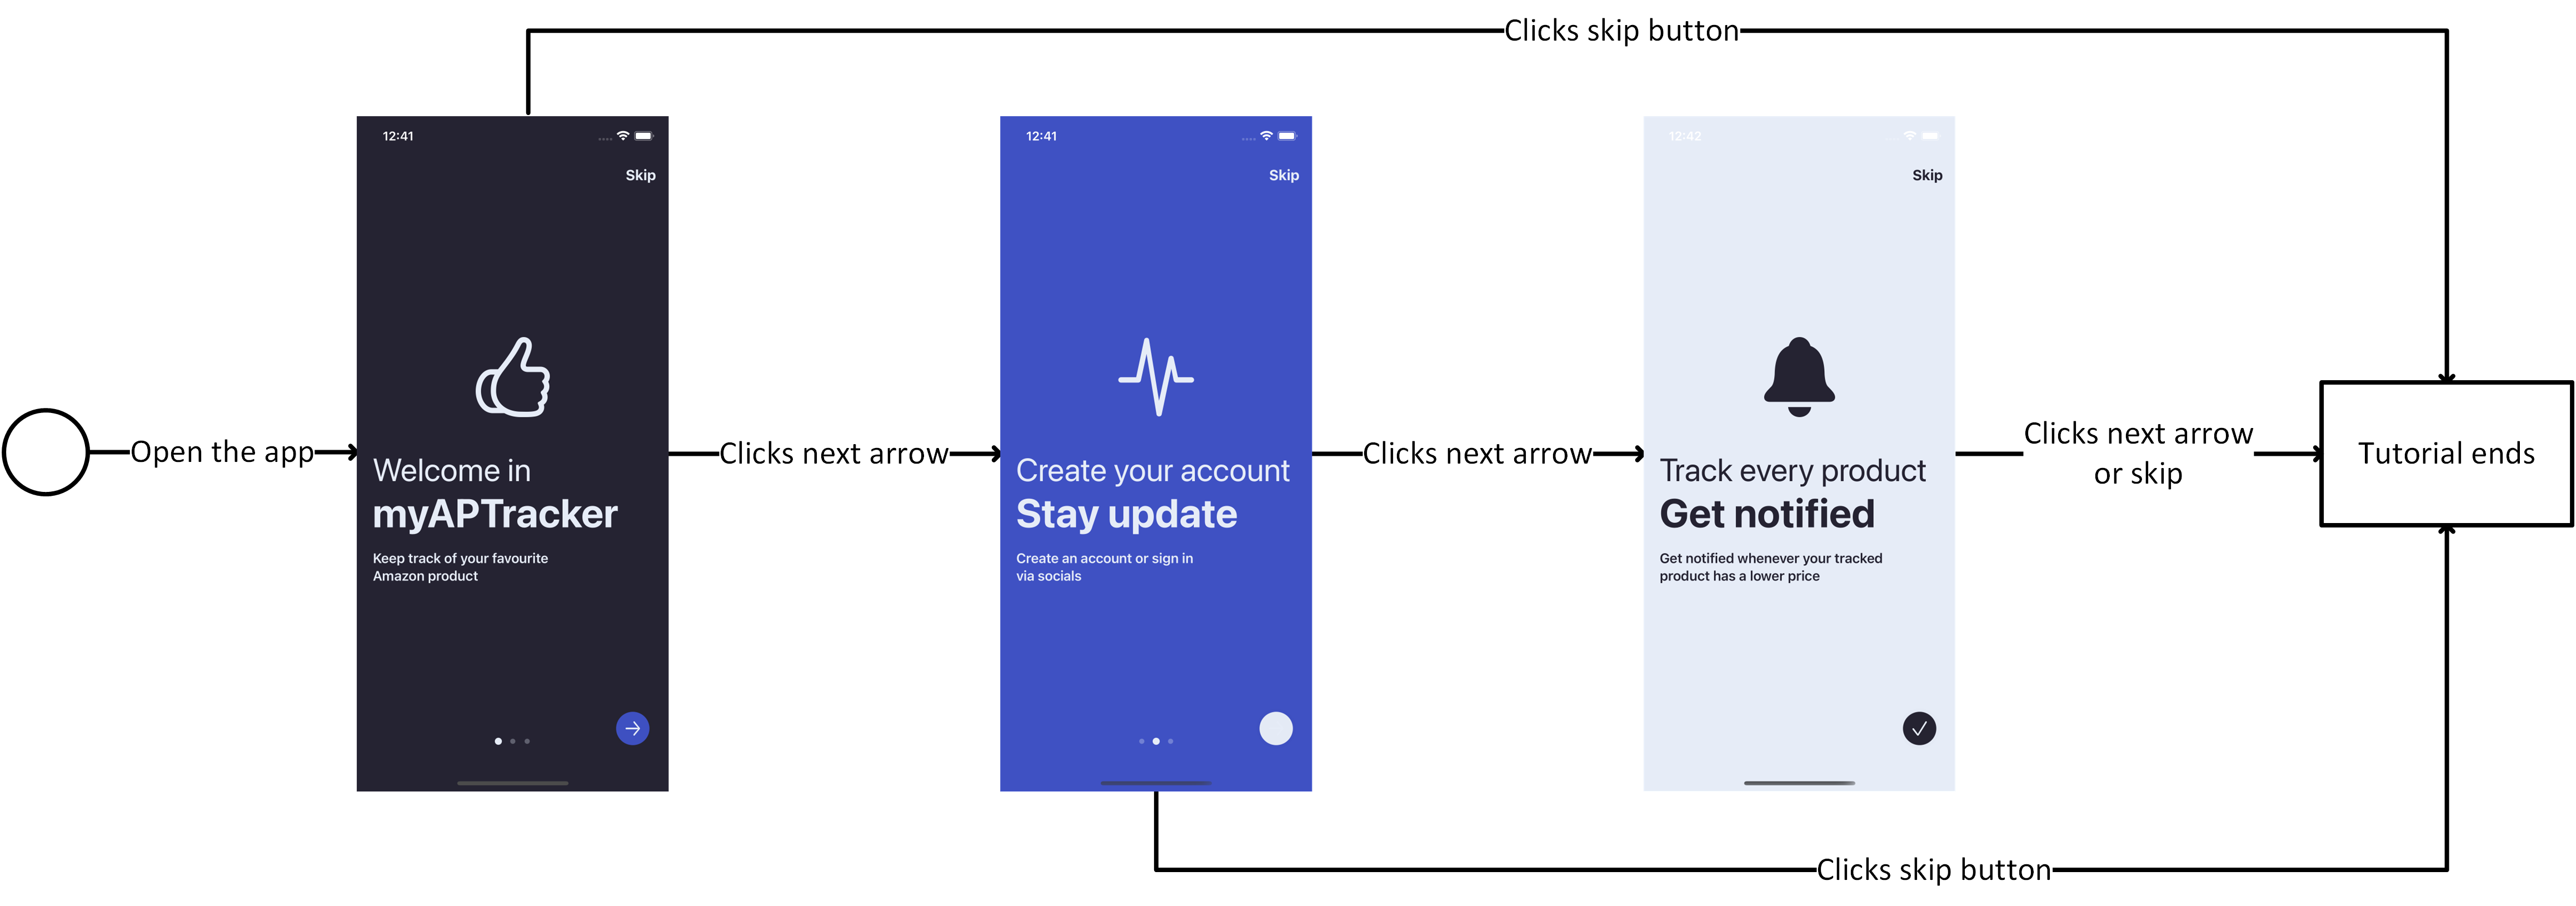
\includegraphics[scale=0.12]{images/interfaces/user_do_tutorial.png}
        \caption{User do the tutorial}
        \label{fig:user_do_tutorial}
\end{figure}
\FloatBarrier
In this flow (fig: \ref{fig:user_do_tutorial}) the user has just downloaded the application, so the first thing that the app will shown at the first opening is a tutorial of how to use the application. The user can decide to view the complete tutorial or skip it.

\begin{figure}[h!]
        \centering
        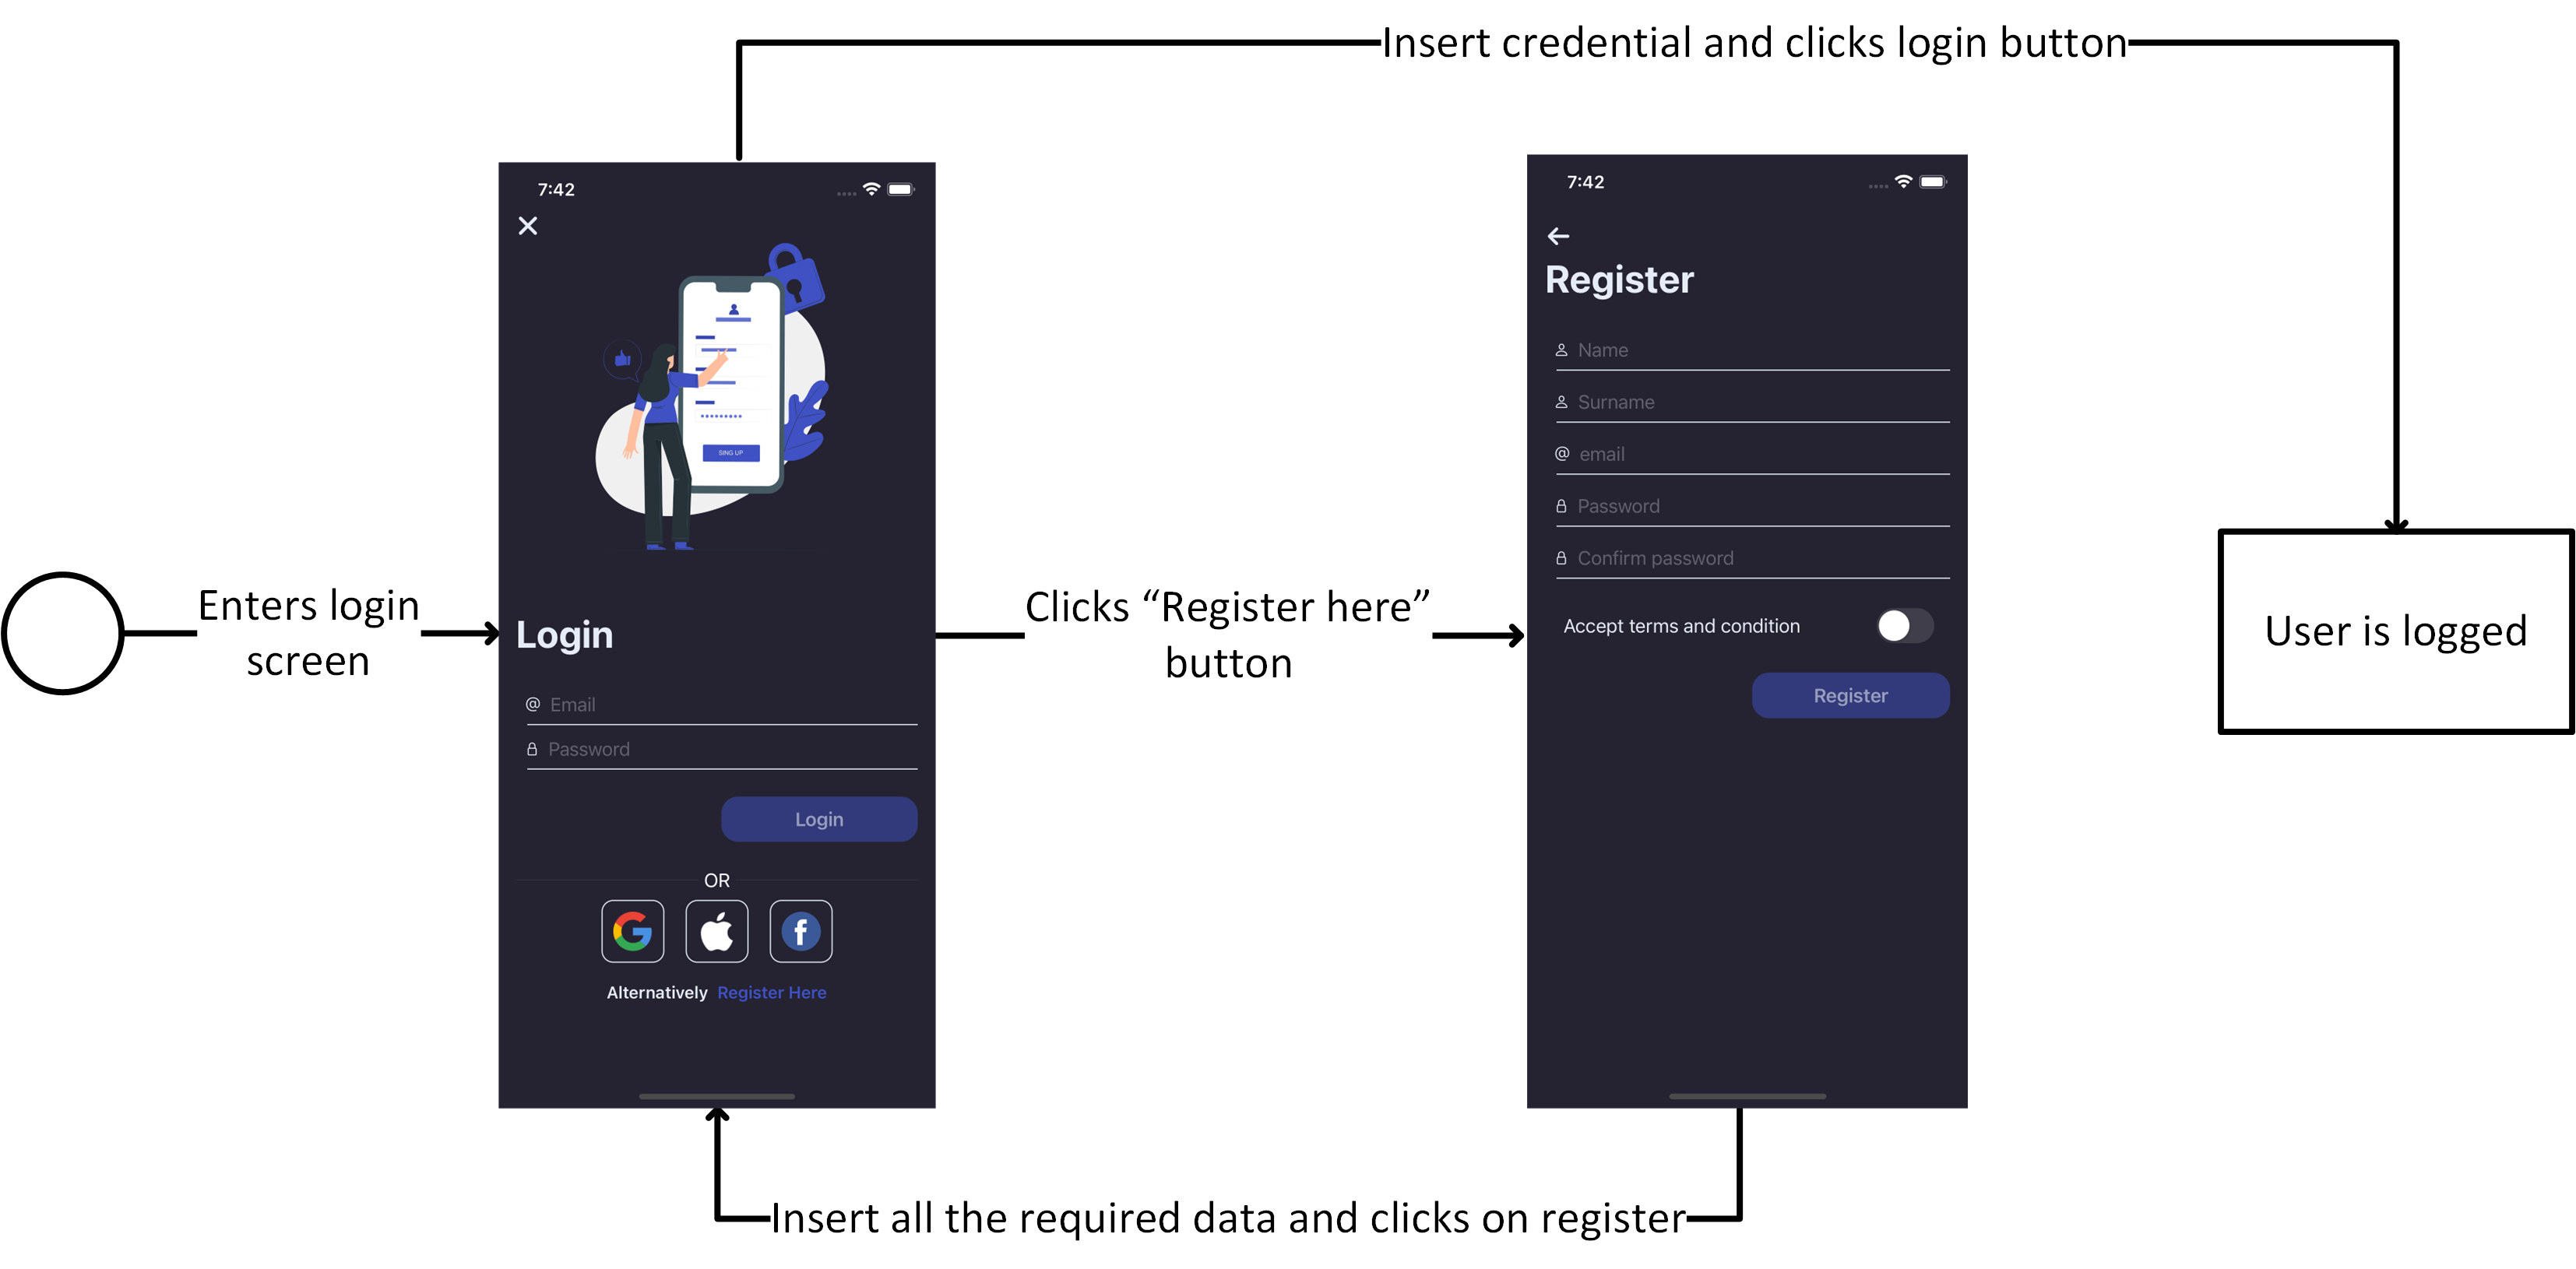
\includegraphics[scale=0.14]{images/interfaces/user_login_interface.png}
        \caption{User register and login locally}
        \label{fig:user_sign_up_and_login}
\end{figure}
\FloatBarrier
In this flow (fig: \ref{fig:user_sign_up_and_login}) the user decide to register to the application, by clicking the register button below the social logos and filling all the requested data. Then he can logs in by inserting the credential that has already listed in the registration phase.\\
If the user has already an account can just insert his credentials and logs in.

\begin{figure}[h!]
        \centering
        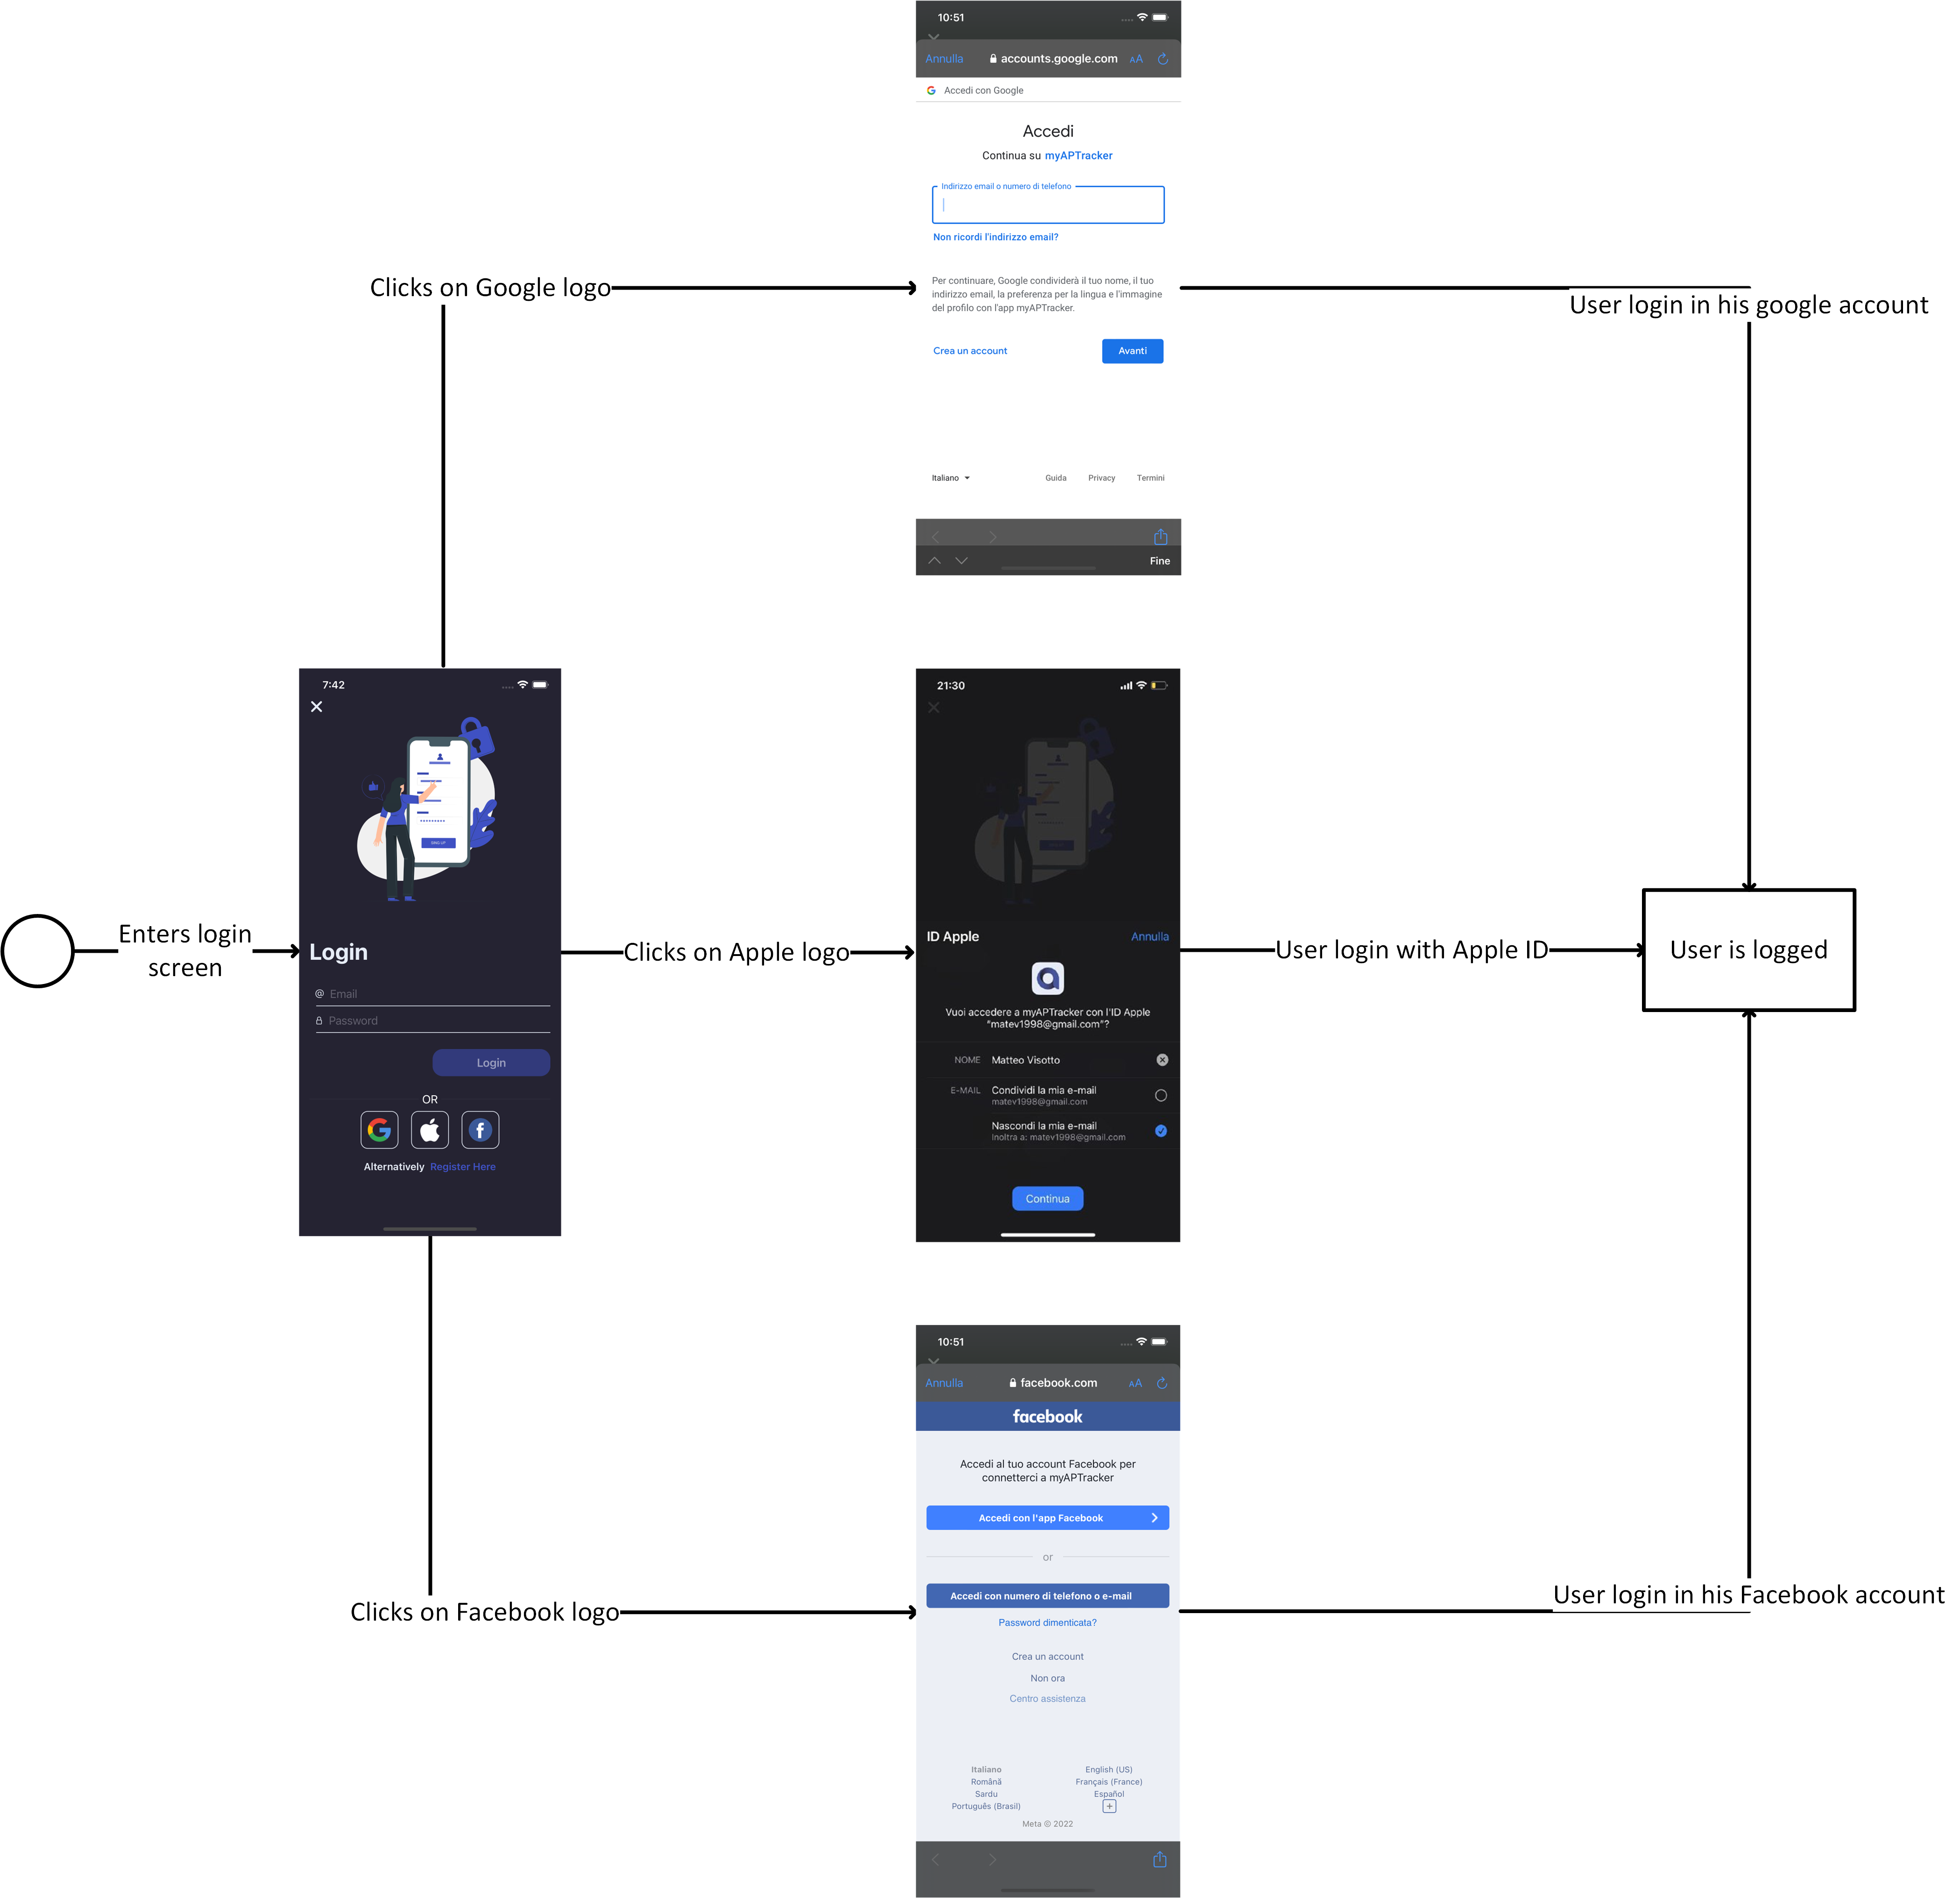
\includegraphics[scale=0.14]{images/interfaces/user_login_interface_social.png}
        \caption{User register and login with social}
        \label{fig:user_sign_up_and_login_social}
\end{figure}
\FloatBarrier
In this flow (fig: \ref{fig:user_sign_up_and_login_social}) the user decide to authenticate through a social authentication mechanism. In order to do that, the user decide the social from which he wants to be authenticated and do the login process in the social. After that procedure the user is authenticated in the application.

\begin{figure}[h!]
        \centering
        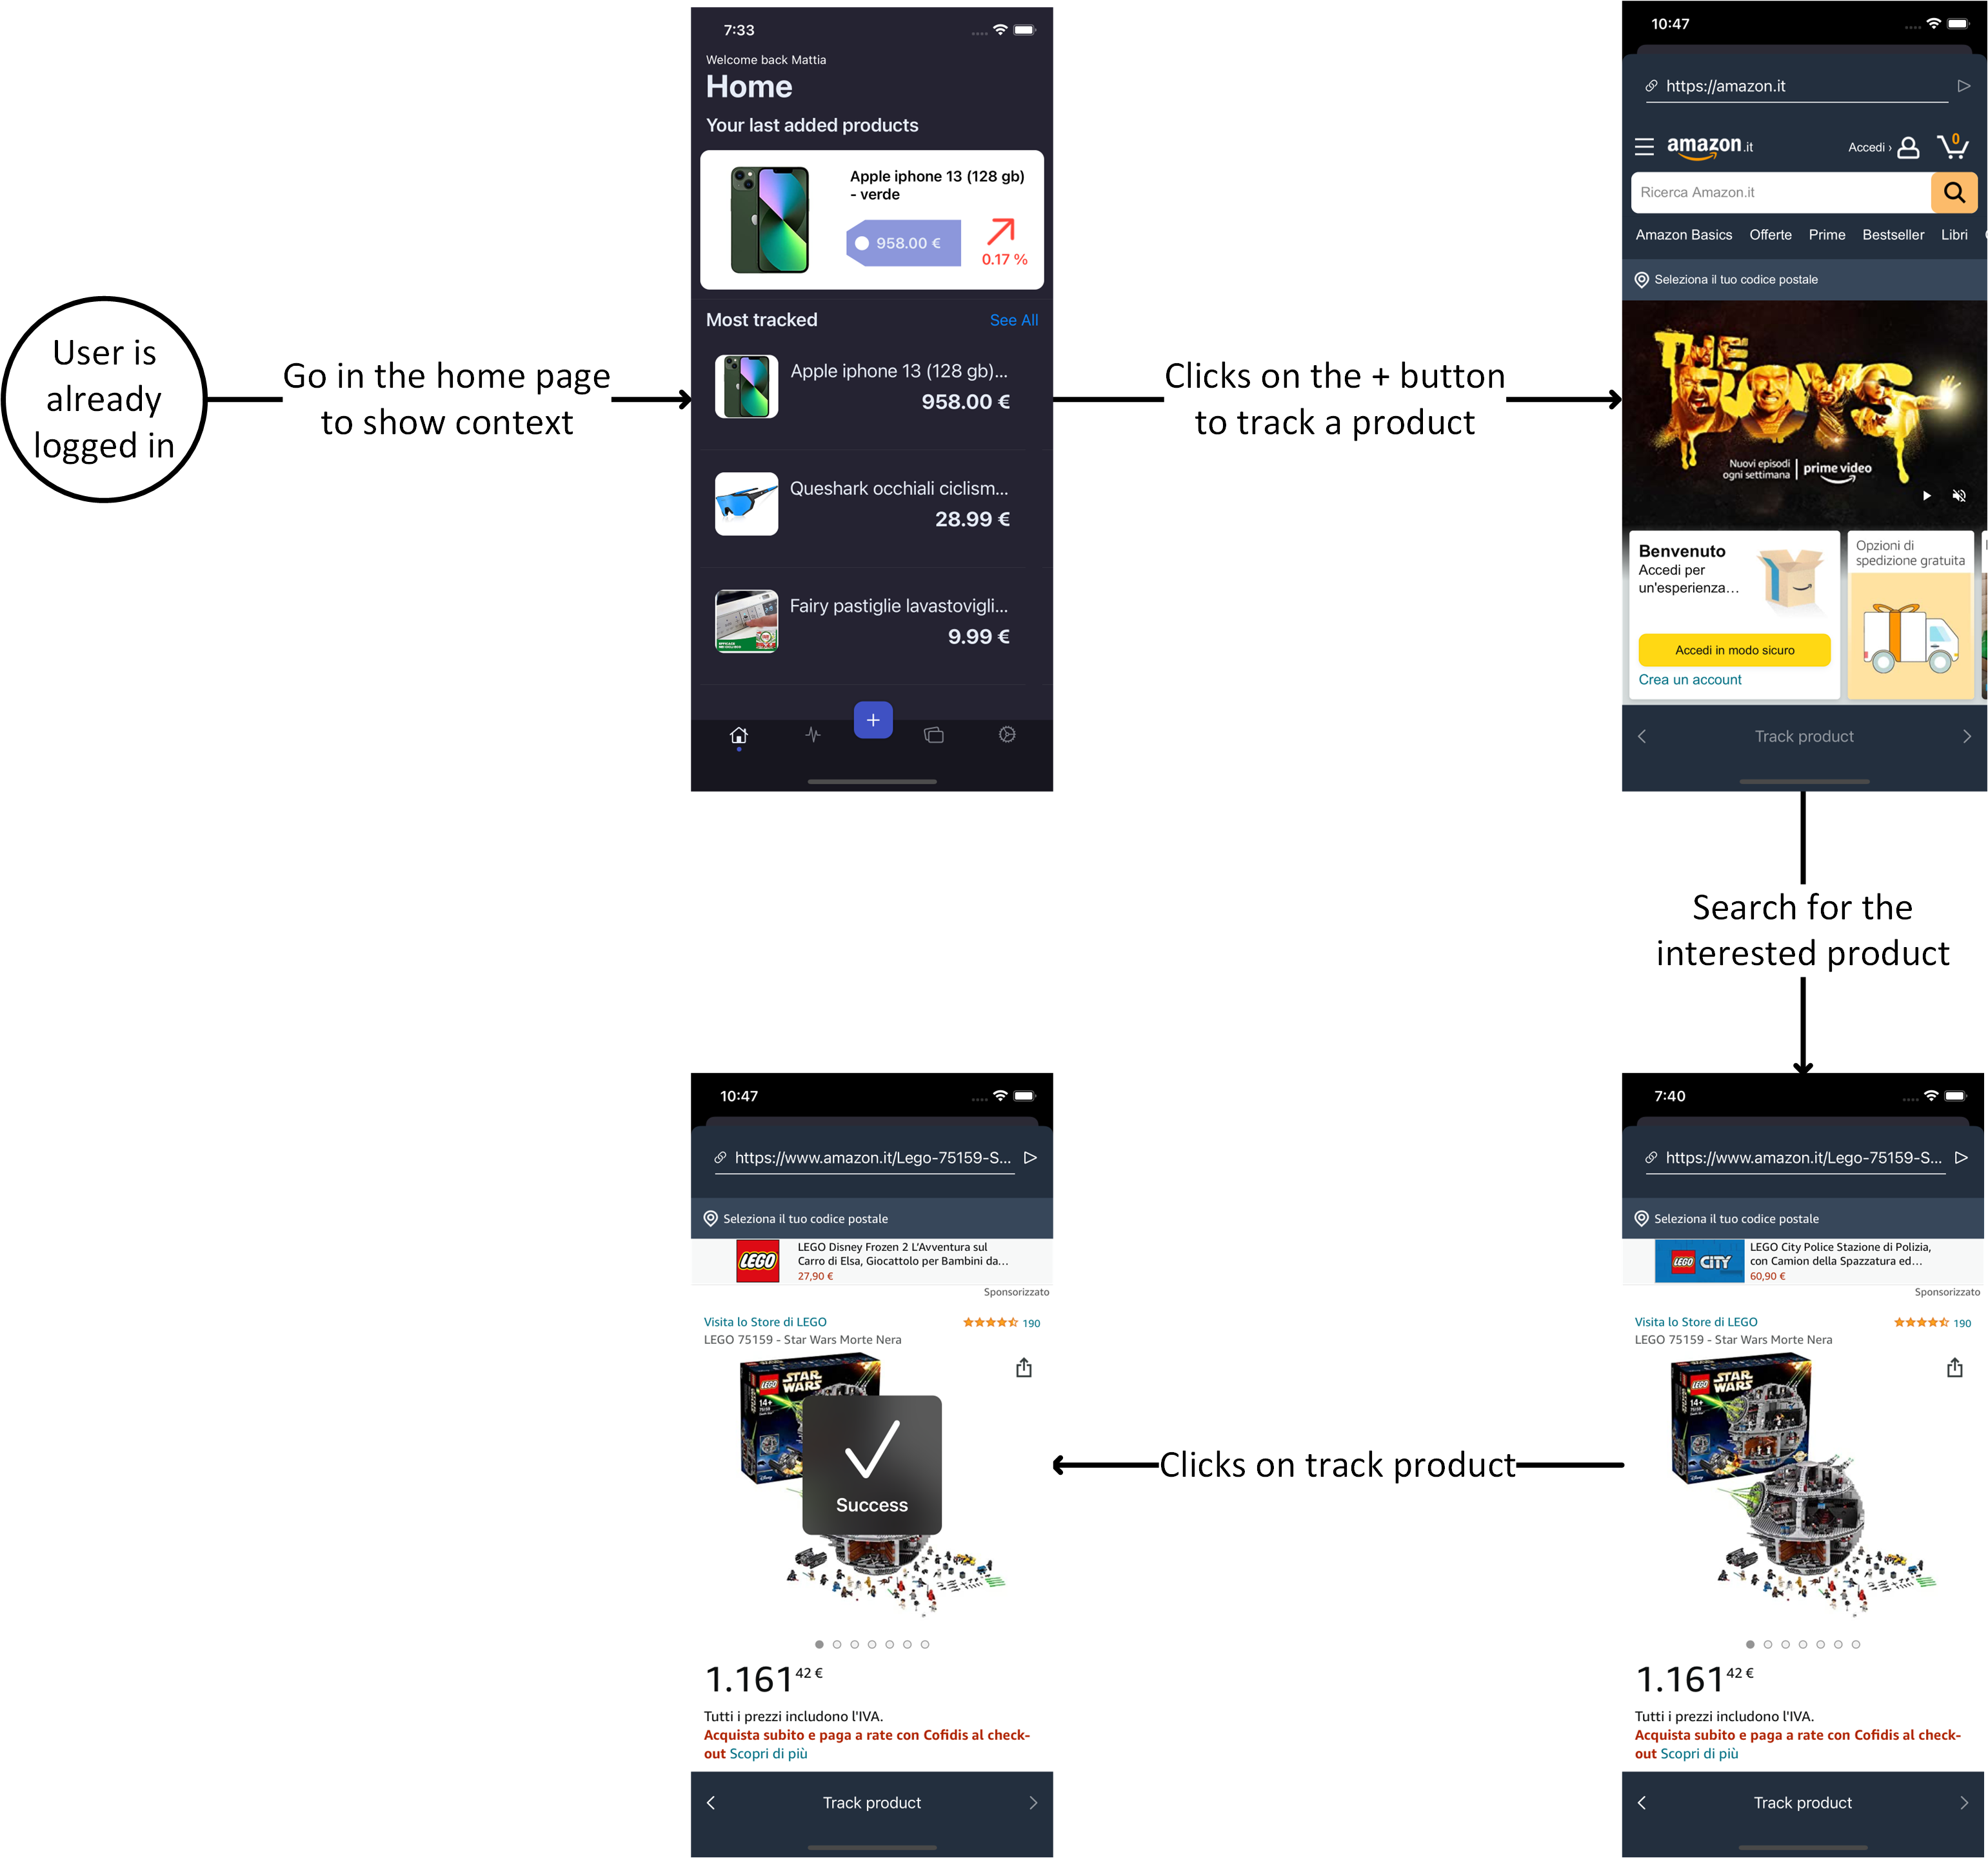
\includegraphics[scale=0.14]{images/interfaces/user_add_track_product.png}
        \caption{User add/track a product}
        \label{fig:user_add_track_product}
\end{figure}
\FloatBarrier
In this flow (fig: \ref{fig:user_add_track_product}) the user decide to track a new product. In order to do that, the user clicks on the plus button present in the bottom tab bar and a sheet will open containing a WebView of the Amazon Homepage (in the iPad the position of the button is different how we will see later). Then a user can search for the product he is interested in and, once reached the product page, he can track it by clicking the "track" button on the bottom.

\begin{figure}[h!]
        \centering
        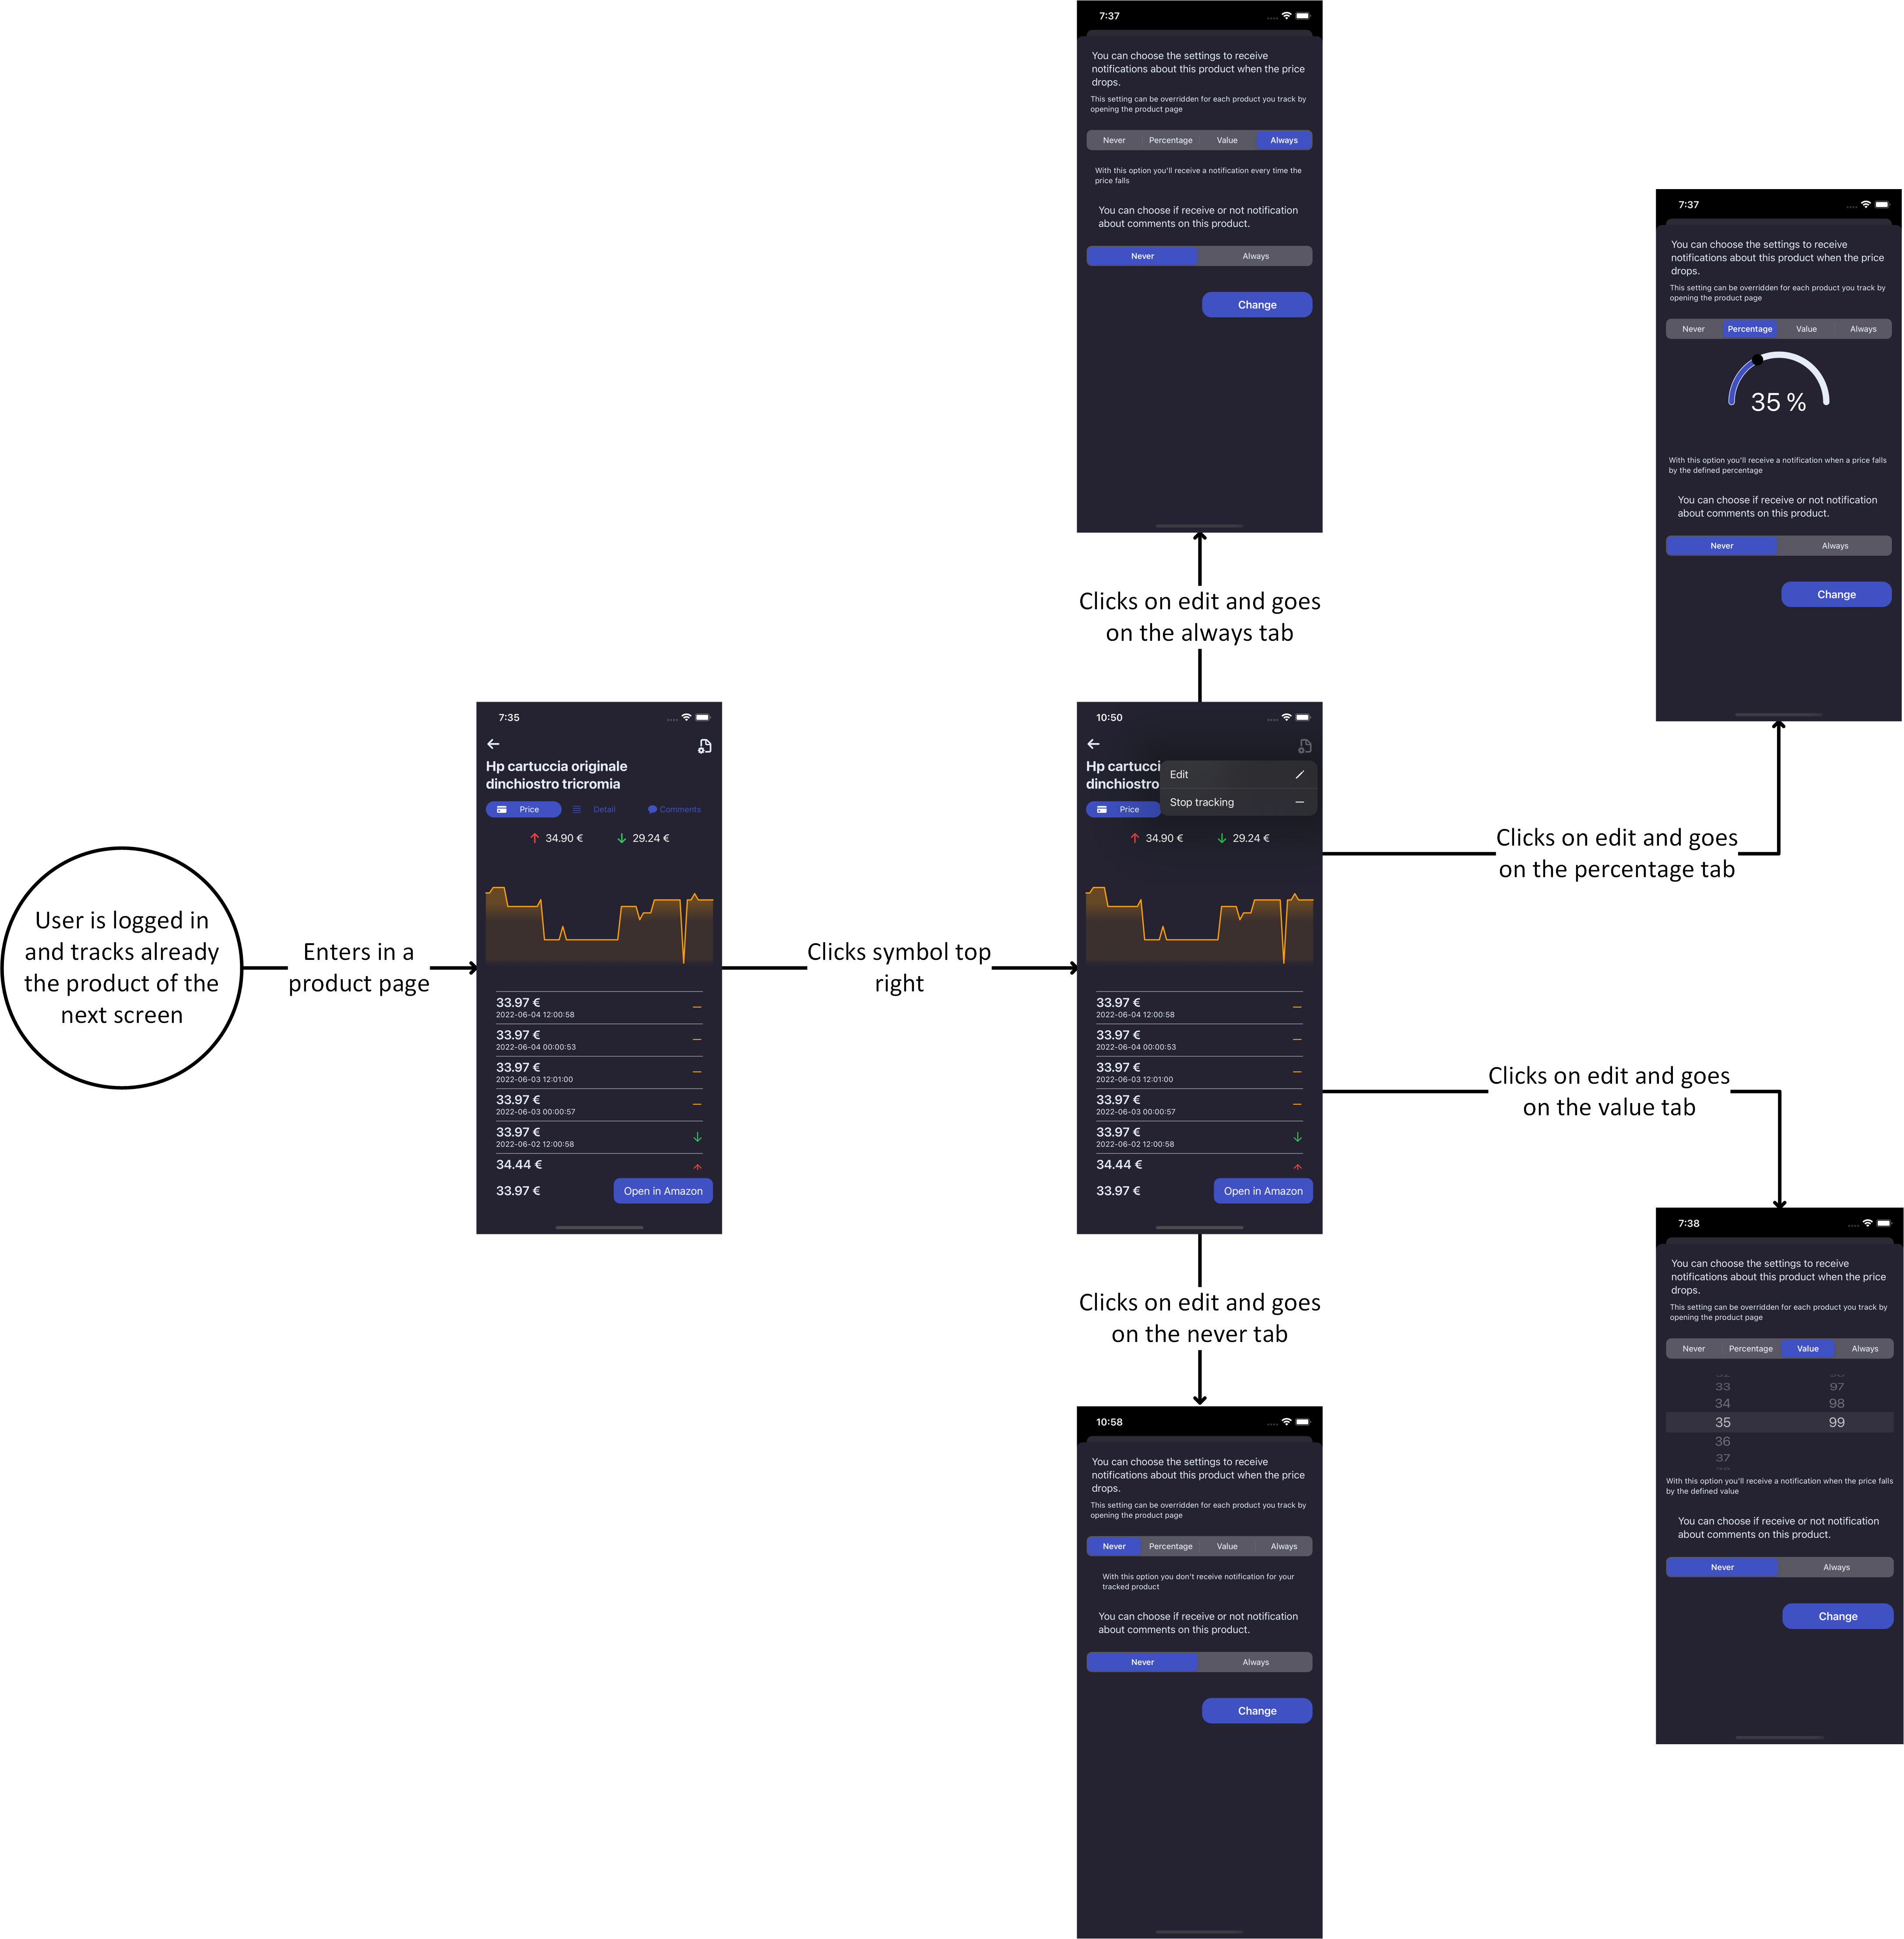
\includegraphics[scale=0.12]{images/interfaces/user_set_range_for_notification.png}
        \caption{User set a range to a product in order to receive a notification}
        \label{fig:user_set_range_for_notification}
\end{figure}
\FloatBarrier
In this flow (fig: \ref{fig:user_set_range_for_notification}) the user decide to modify the rule under which he receives a notification for a specific product. In order to do that, the user enters in the product page, clicks the symbol in the top right and then choose to edit the product settings.\\
At this point the can choose 4 different types of possible notification:
\begin{itemize}
    \item \textbf{Always:} every time the price change the user will receive a notification for this product.
    \item \textbf{Never:} the user will never receive a notification for this product.
    \item \textbf{Percentage:} every time the price goes below a certain percentage (from the price present when the notification setting was saved), the user will receive a notification for this product.
    \item \textbf{Value:} every time the price goes below a certain price, the user will receive a notification for this product.
\end{itemize}
Finally, the user can also choose to receive or not the notification on comments about that product and save the settings by clicking on change.

\begin{figure}[h!]
        \centering
        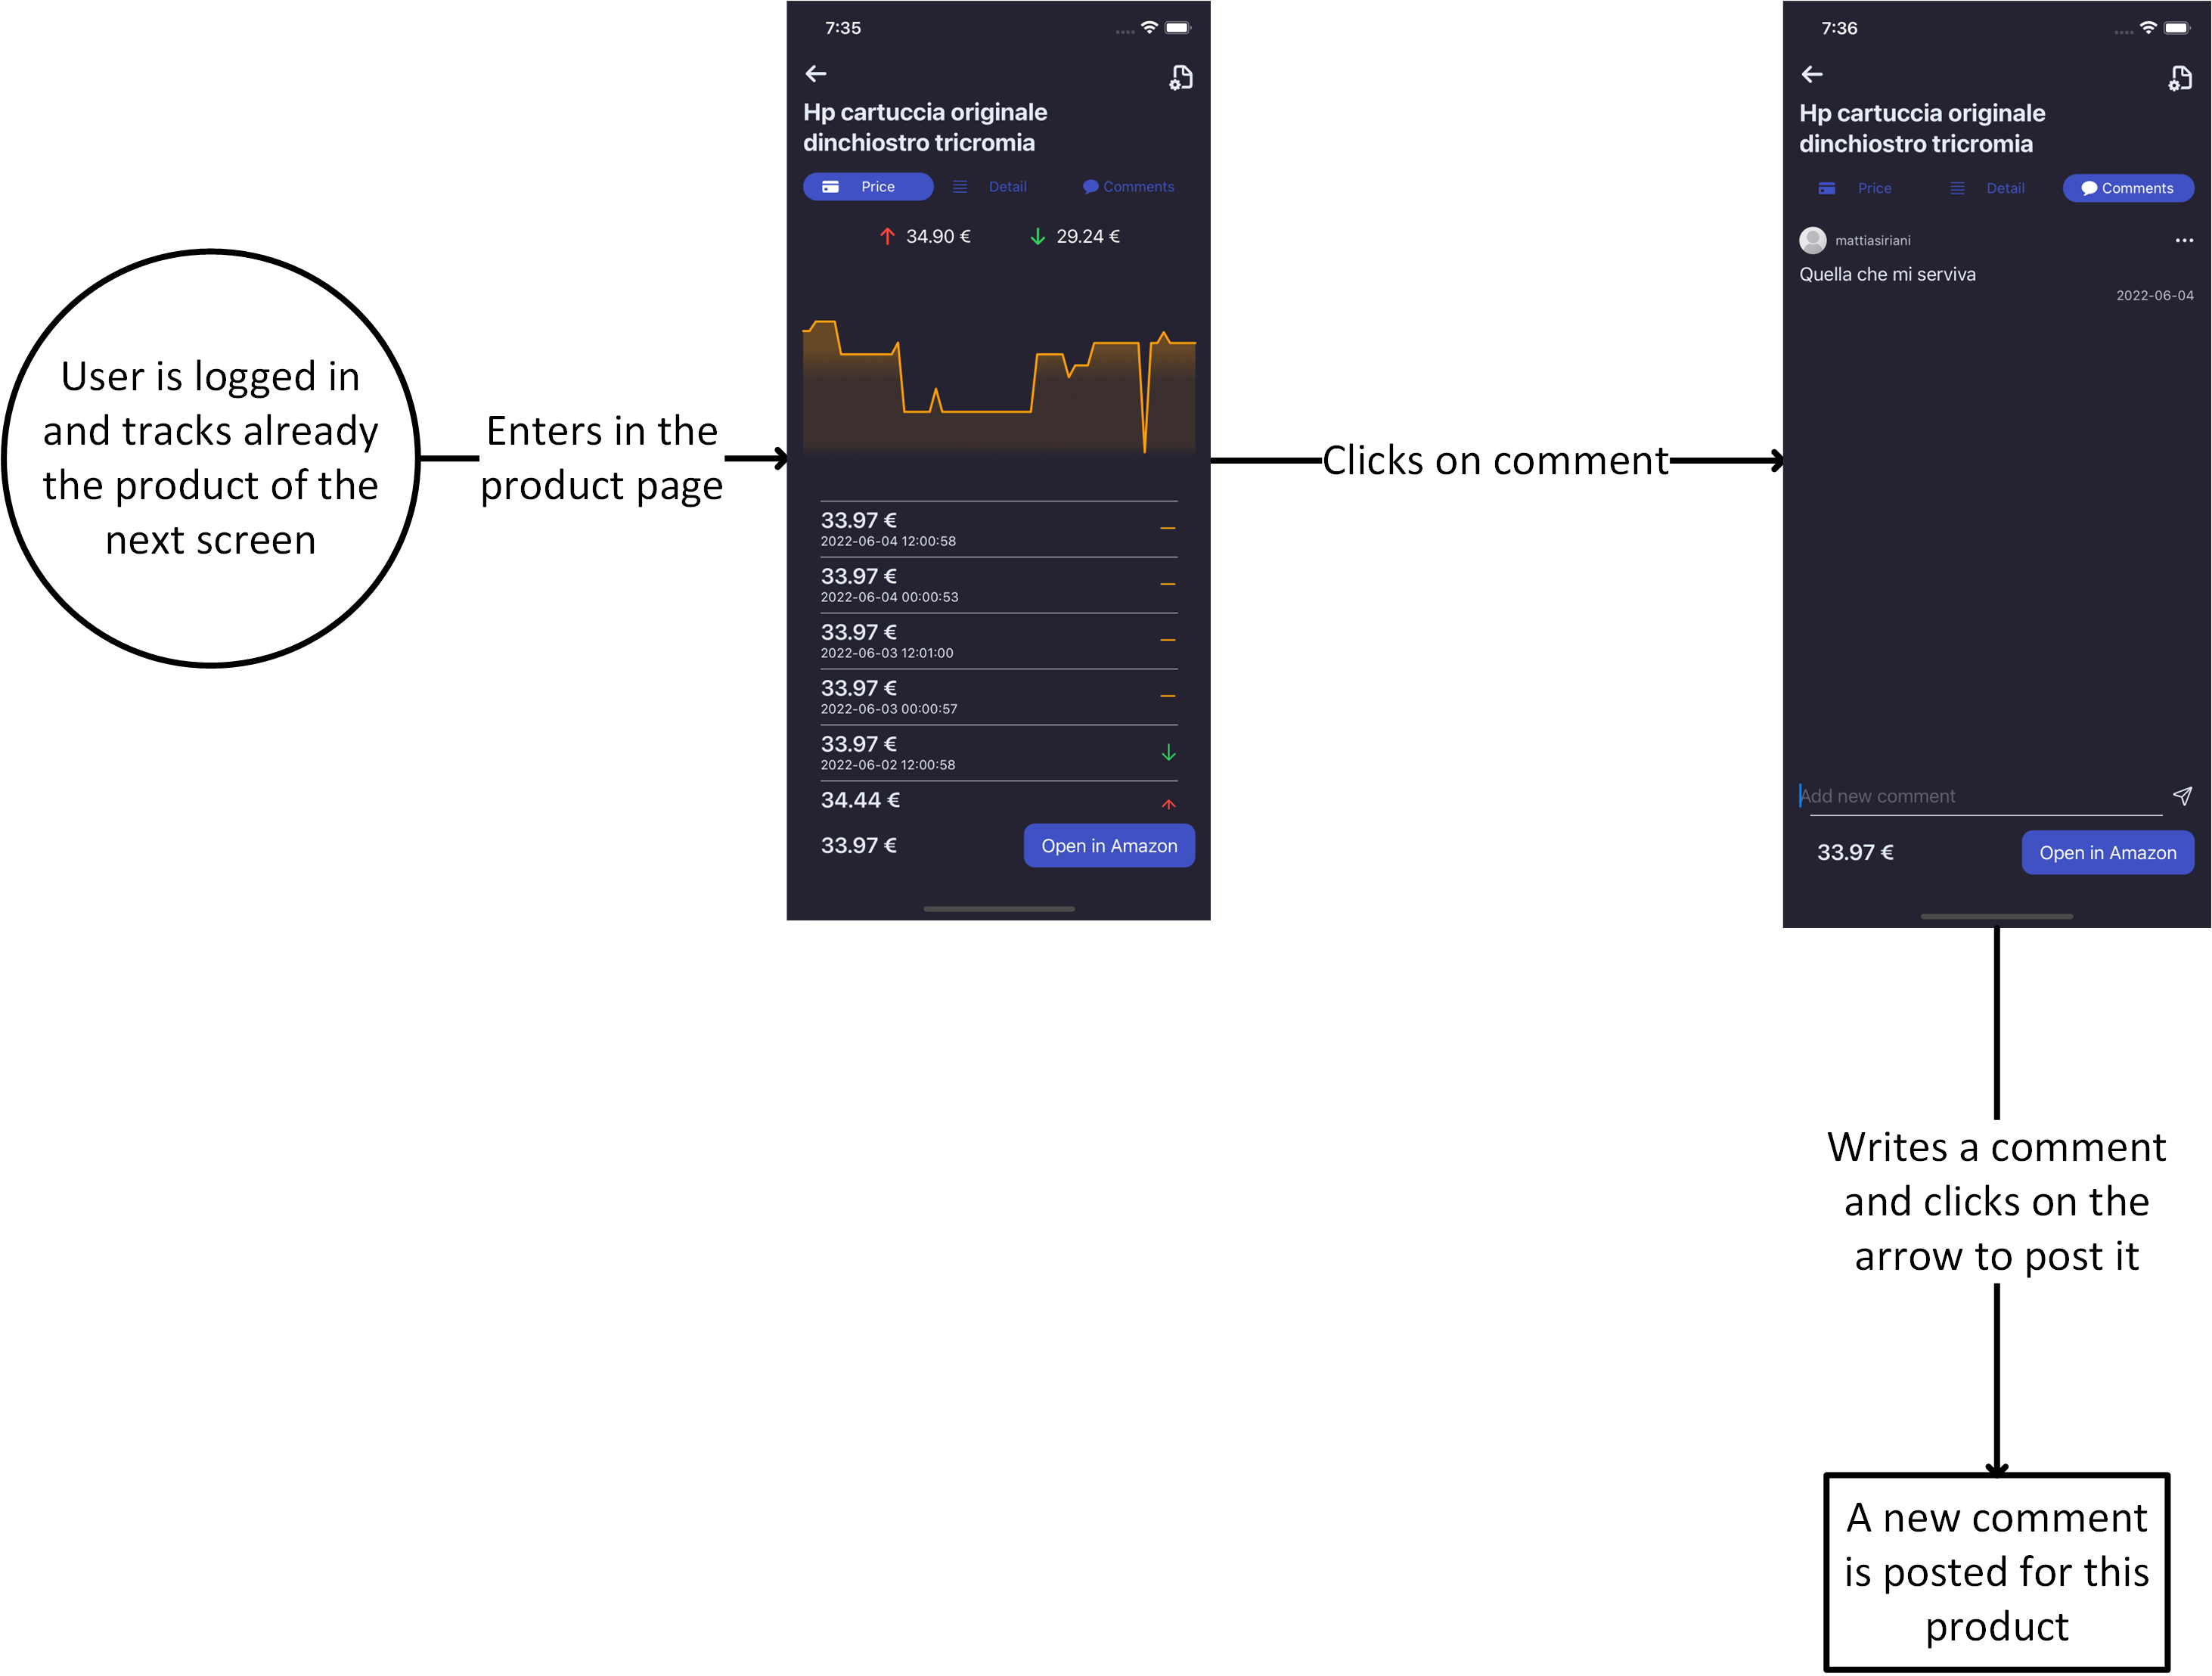
\includegraphics[scale=0.14]{images/interfaces/user_post_comment.png}
        \caption{User post a comment for a product}
        \label{fig:user_post_comment}
\end{figure}
\FloatBarrier
In this flow (fig: \ref{fig:user_post_comment}) the user wants to post a comment about a specific product. In order to do that, the user enters in the product page and goes on the comment section. After done that, the user writes what he wants to say about this specific product and then click the arrow on the right to post it. The page will redraw and the user comment will be present in the page.

\begin{figure}[h!]
        \centering
        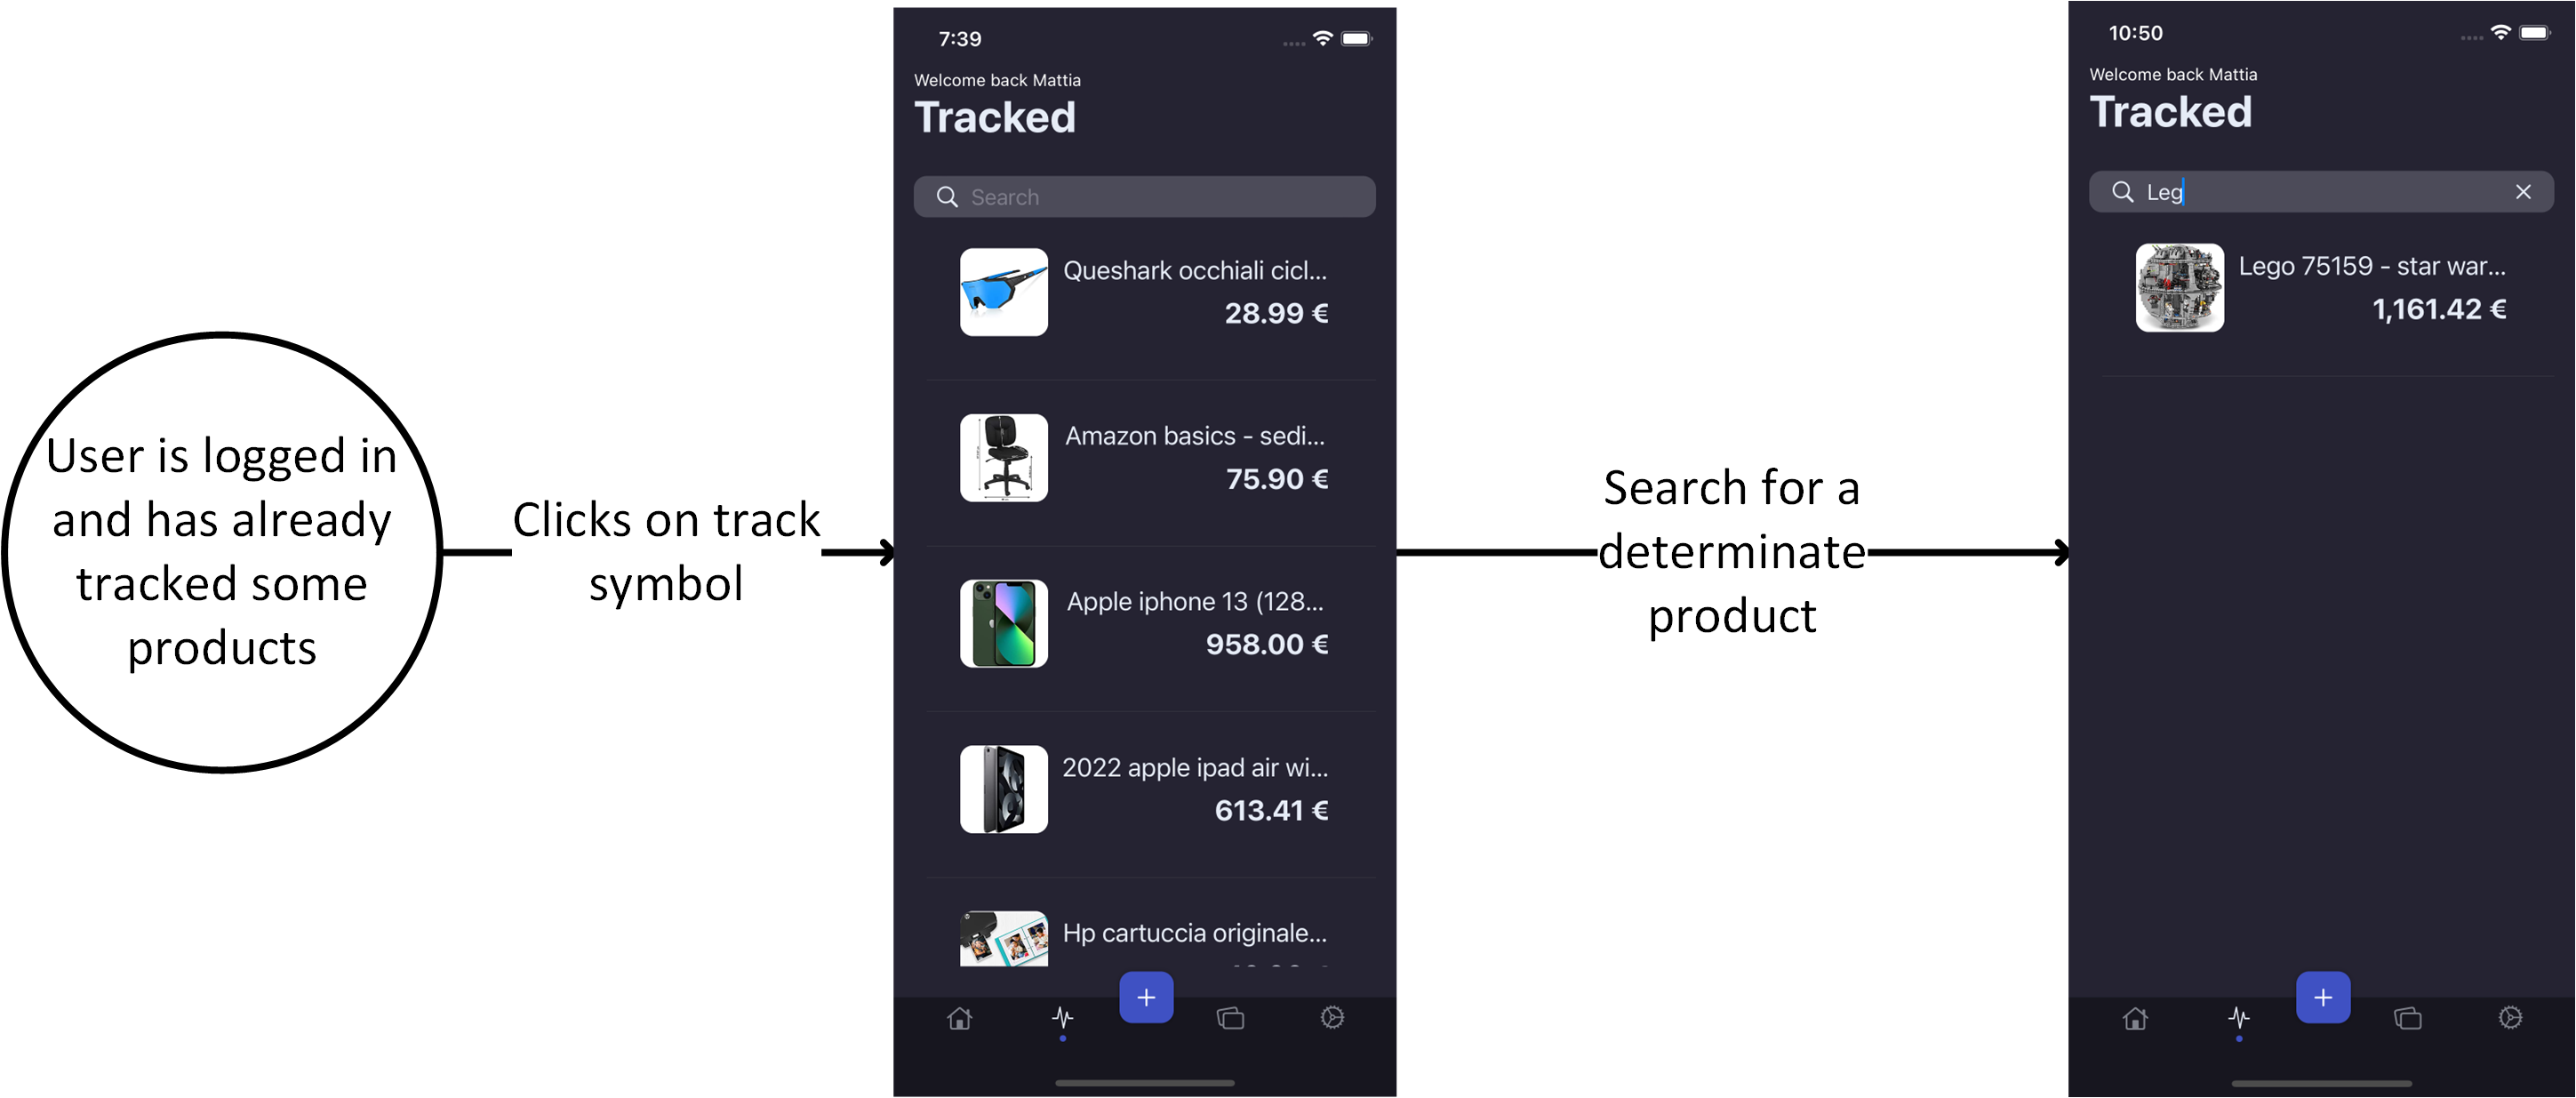
\includegraphics[scale=0.14]{images/interfaces/user_search_in_tracked.png}
        \caption{User search a product between all the products that he has tracked}
        \label{fig:user_search_in_tracked}
\end{figure}
\FloatBarrier
In this flow (fig: \ref{fig:user_search_in_tracked}) the user wants to search a product that he has already tracked, in order to see it. To do that, the user goes in the tracking section, present in the bottom navigation bar and at this point he will type the name of the product he is interested in and all the products that correspond to the search will be shown.

\begin{figure}[h!]
        \centering
        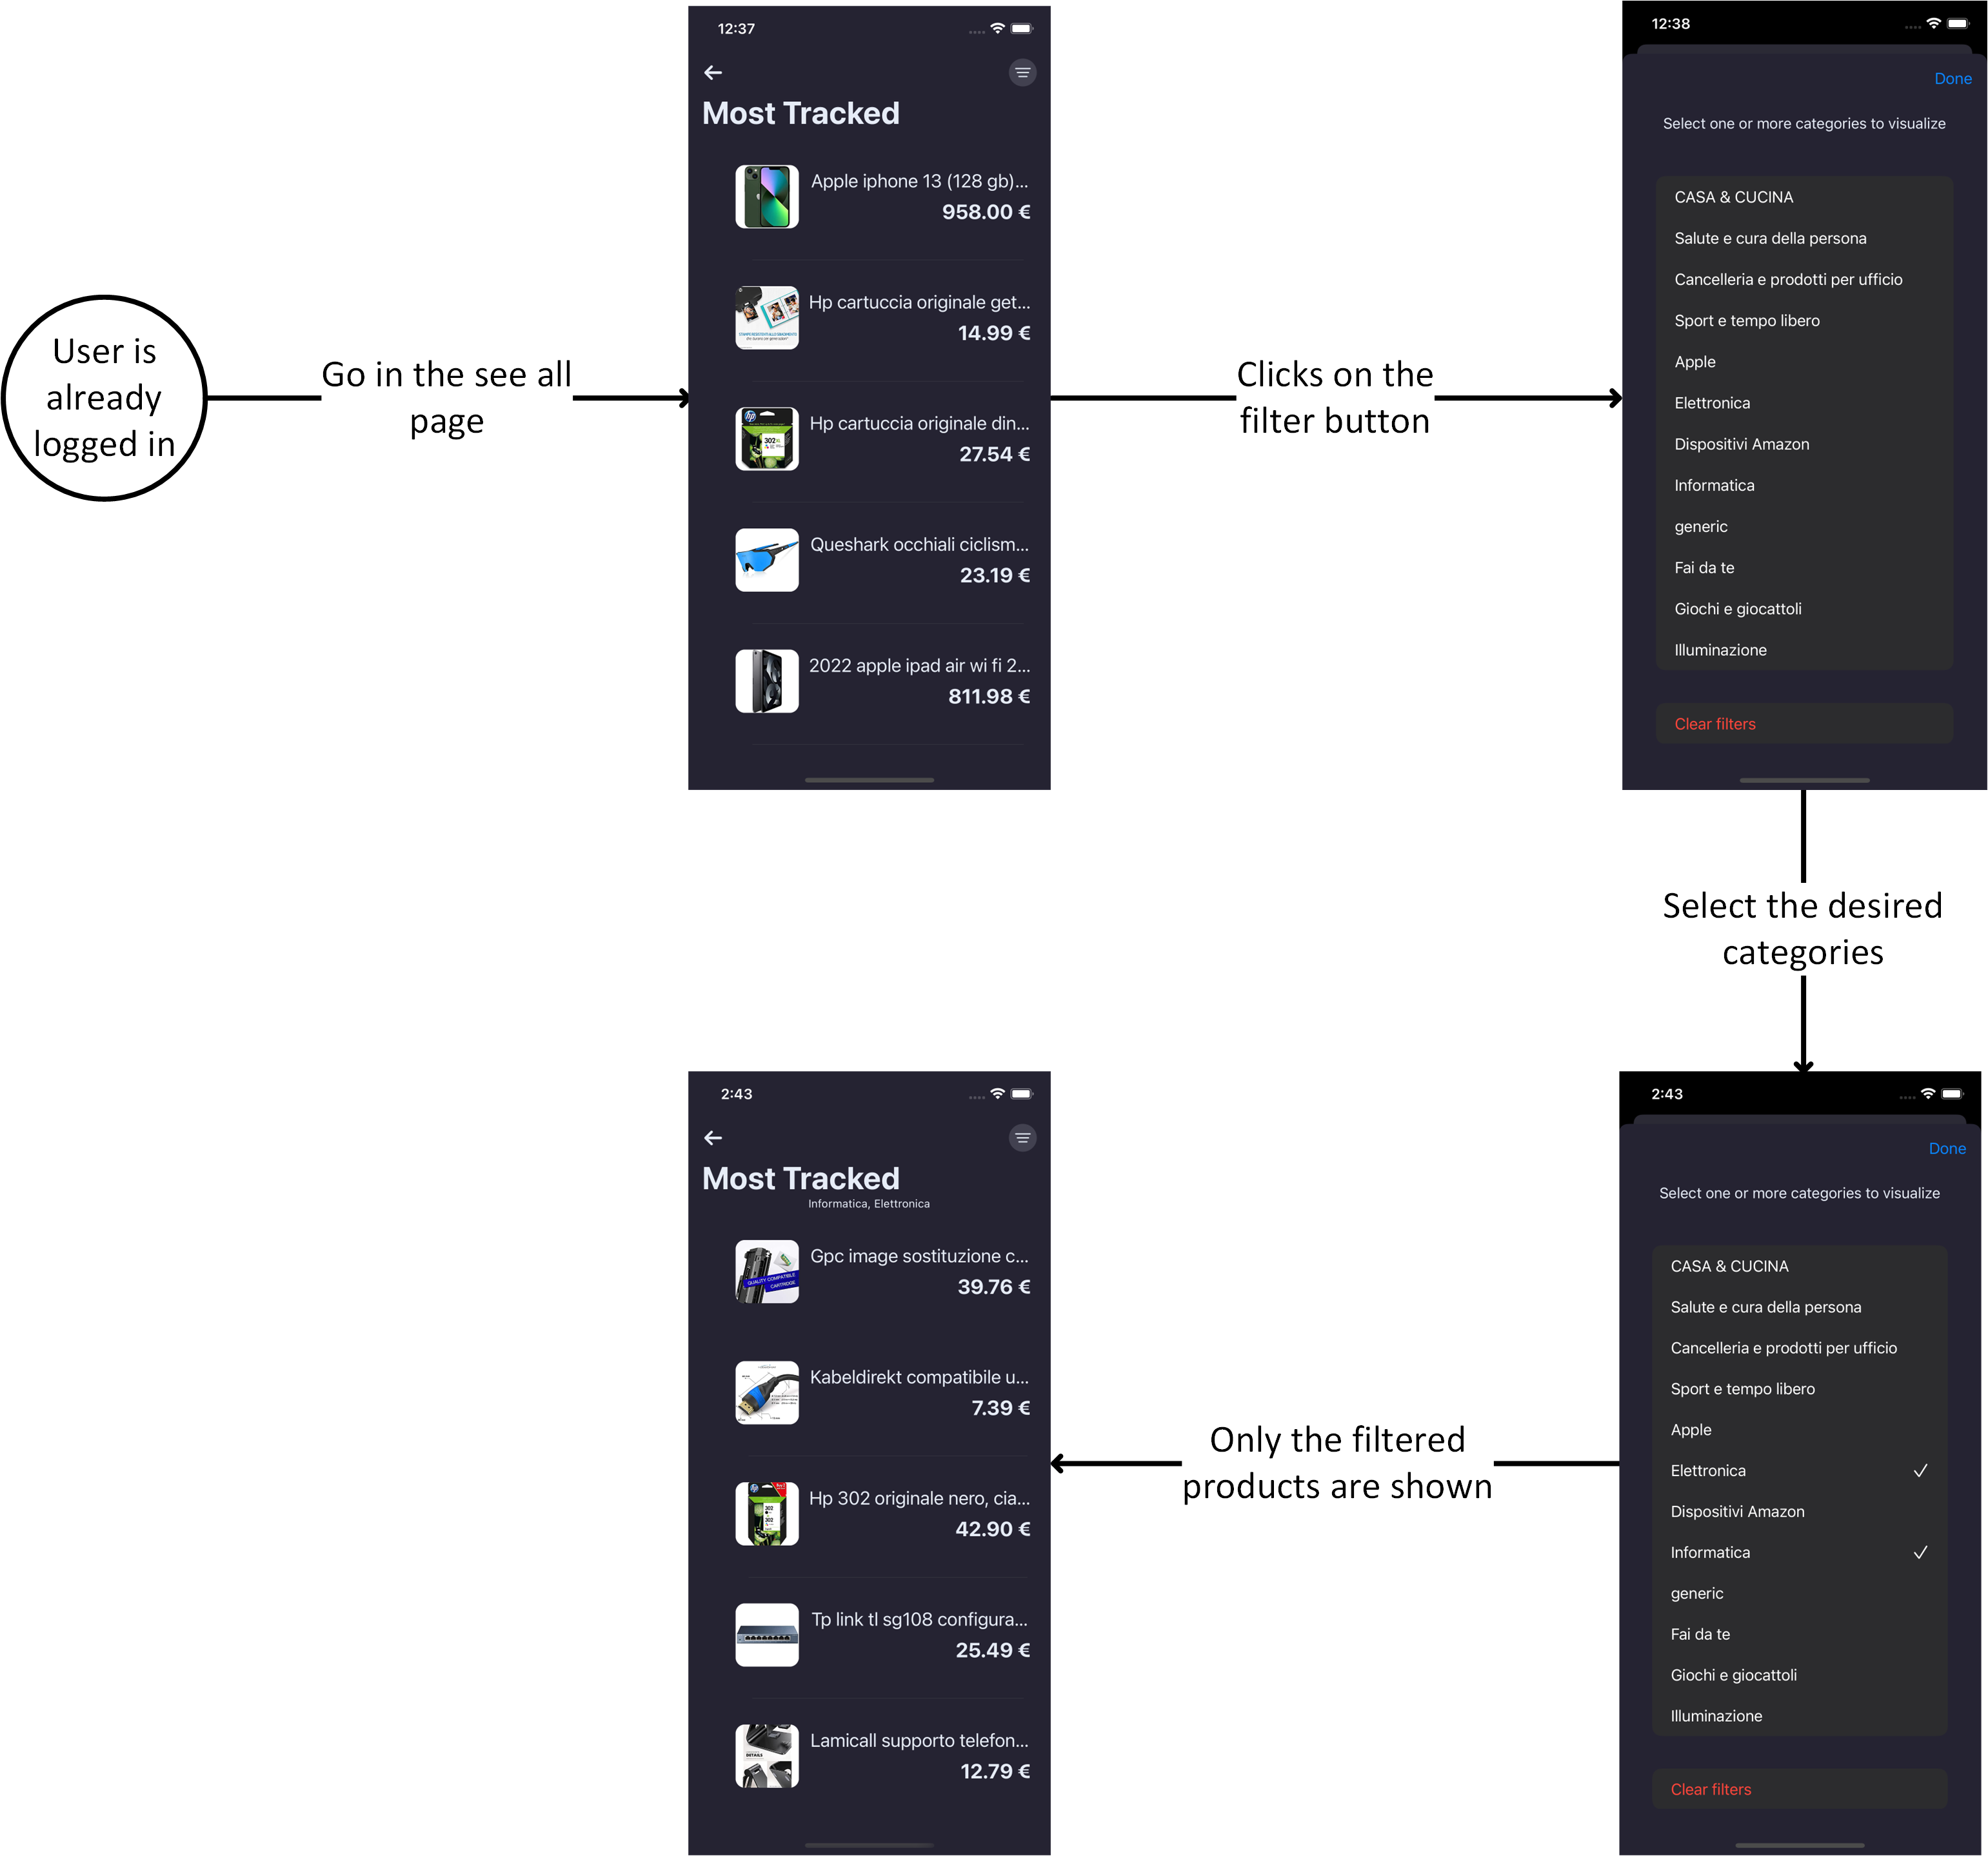
\includegraphics[scale=0.14]{images/interfaces/user_filter_category.png}
        \caption{User filter by category}
        \label{fig:user_filter_category}
\end{figure}
\FloatBarrier
In this flow (fig: \ref{fig:user_filter_category}) the user wants to see only a certain subset of categories of products in the the see all view. In order to do that, the user decide to click on the filter button in the top right corner of the screen and at that point a sheet will be opened, showing the different categories from which the user could choose.\\
At this point the user selects a subset of categories he wants to visualize.\\
Finally, the user has to click on the confirmation button in the top right corner and the chosen subset will be shown.

\begin{figure}[h!]
        \centering
        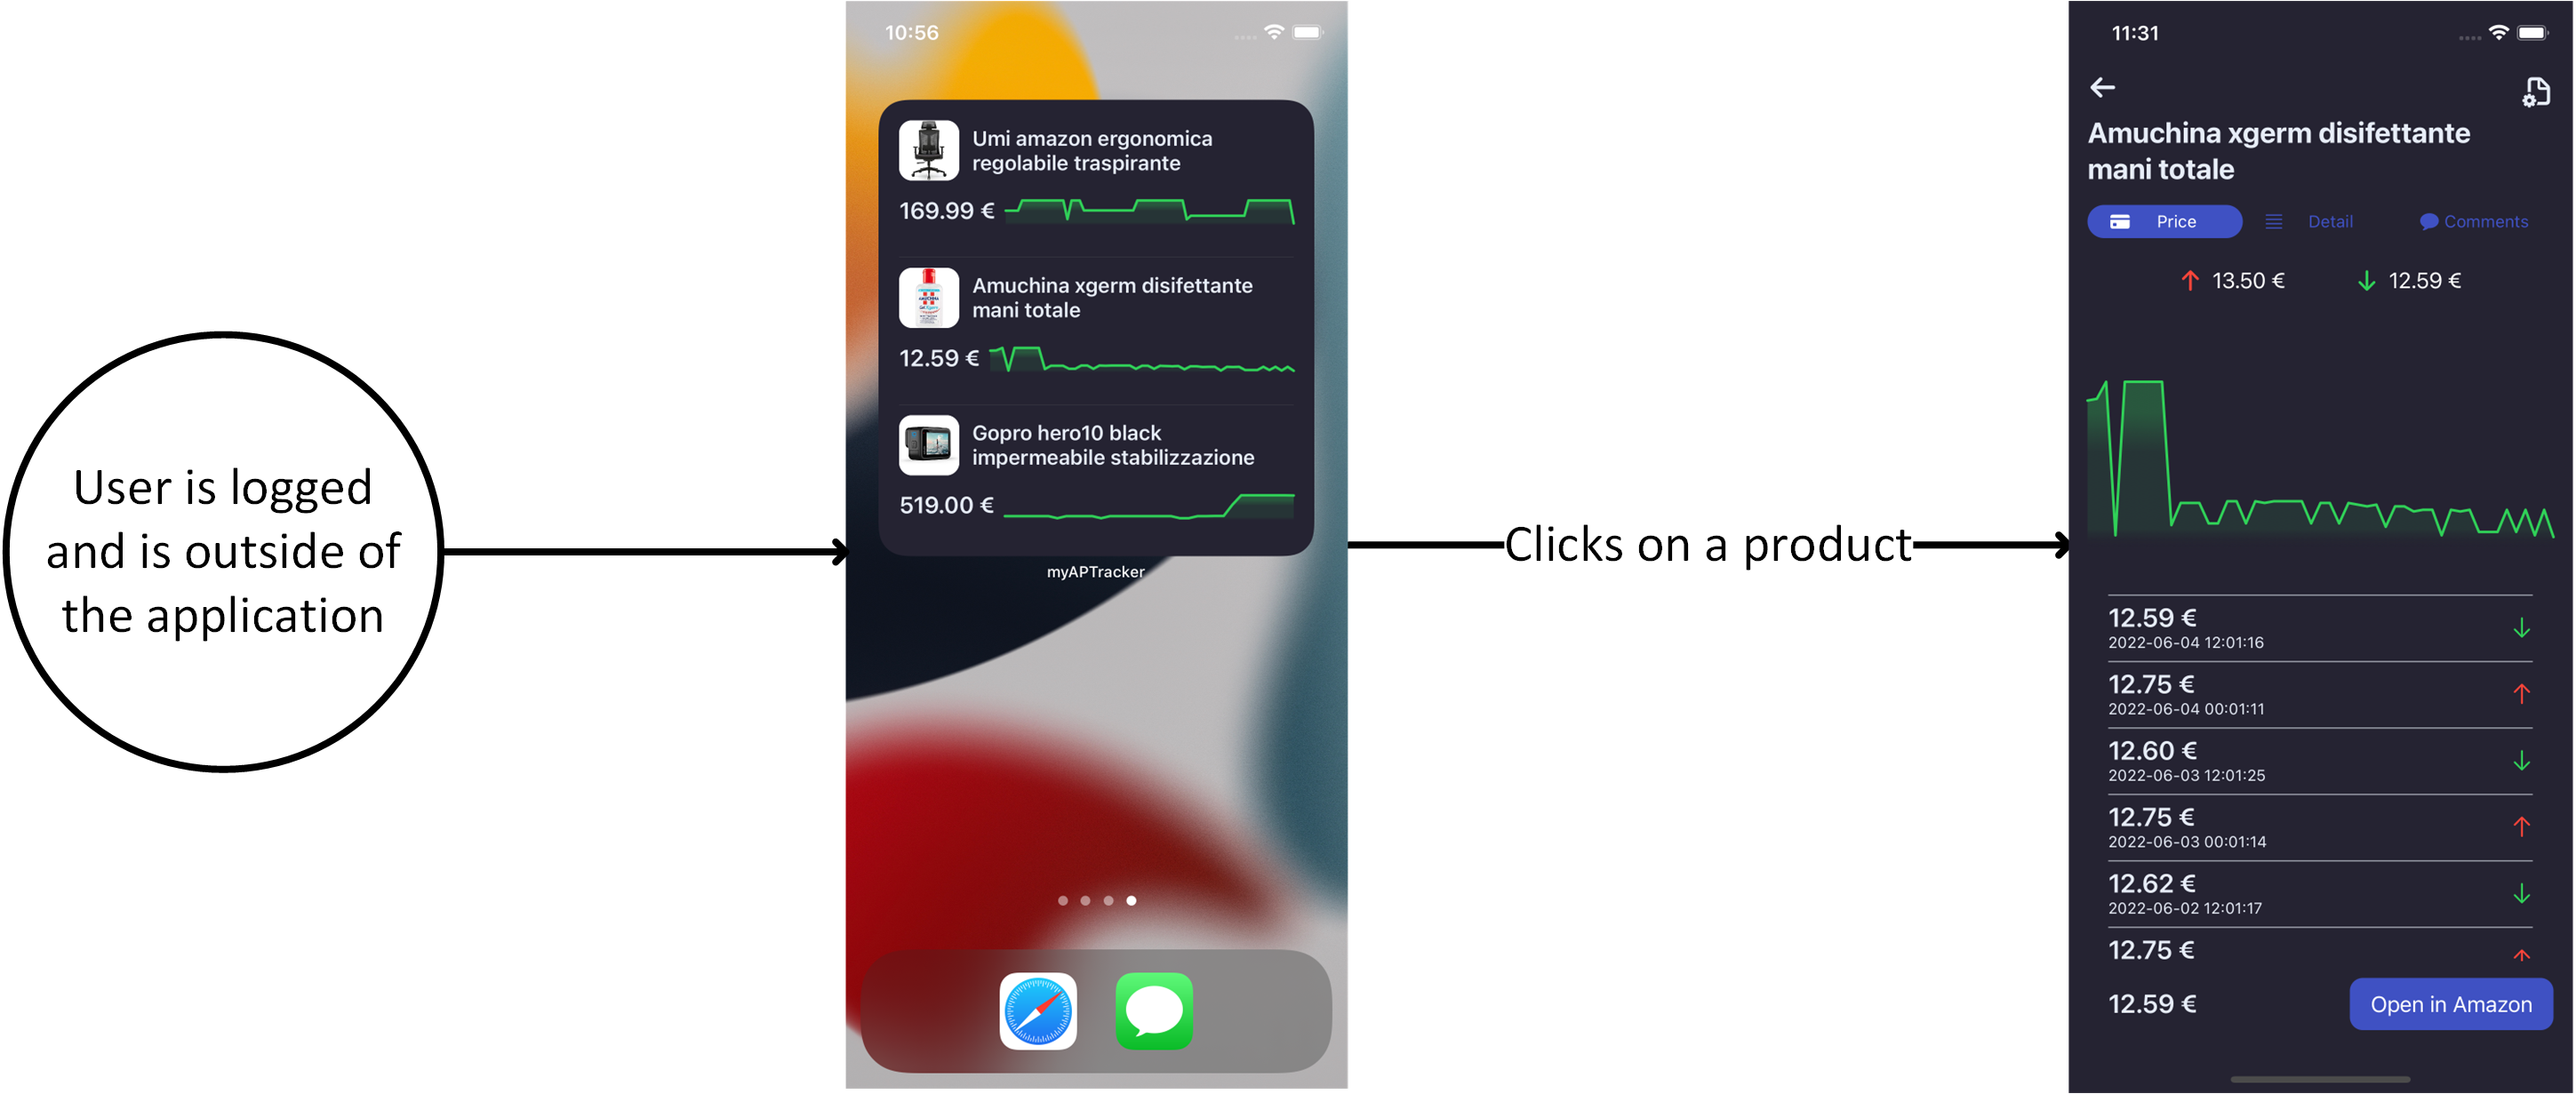
\includegraphics[scale=0.14]{images/interfaces/user_use_widget.png}
        \caption{User use a widget}
        \label{fig:user_use_widget}
\end{figure}
\FloatBarrier
In this flow (fig: \ref{fig:user_use_widget}) the user wants to see a product because he saw from the widget that the product has had a price drop. In order to do that, the user clicks on the product he is interested in and myAPTracker will open and show the product clicked.


\newpage
\subsection{iPhone and iPad screen}
In this section are presented all the view of our application for iPhone and iPad. In order to avoid duplicated images, the views that were equals for both devices are omitted. Finally, though the iPad could handle portrait and landscape, only the portrait views for the iPad are shown below.

\begin{figure}[h!]
        \centering
        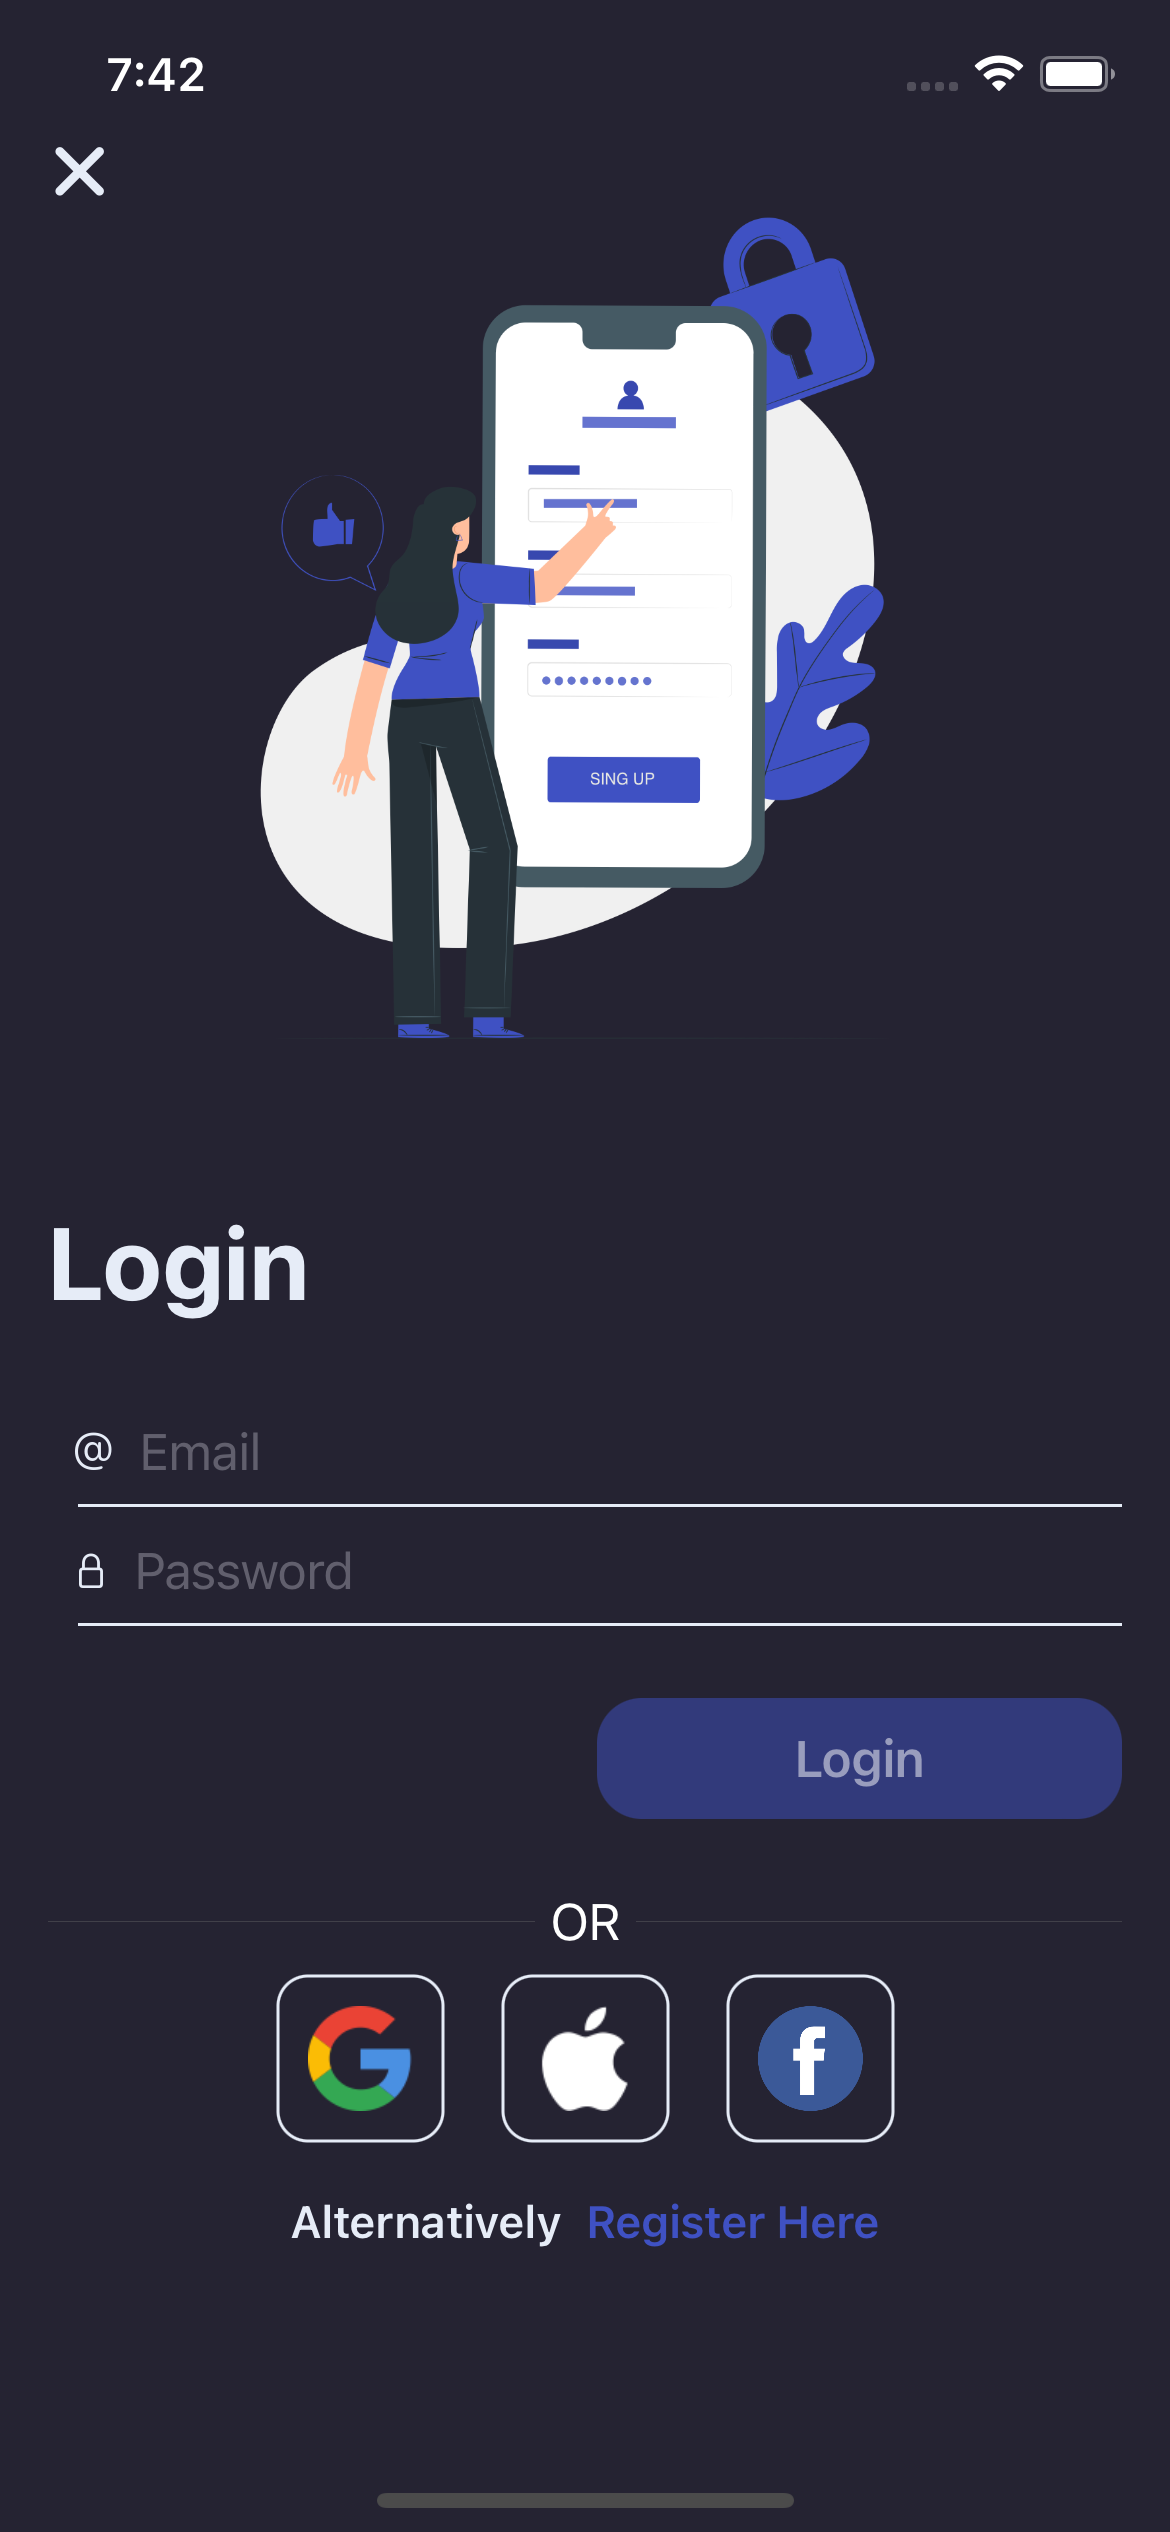
\includegraphics[scale=0.15]{images/interfaces/login_screen.png}
         \caption{Log in screen}
        \label{fig:login_screen}
\end{figure}
\FloatBarrier
This is the login view (fig: \ref{fig:login_screen}). Here the user can login inserting its credential and click on login button. From this page the user can also authenticate by means of social such as Facebook, Google and Apple. Finally, if the user wants to create an account can navigate to the register page with the "Register Here" button.

\begin{figure}[h!]
        \centering
        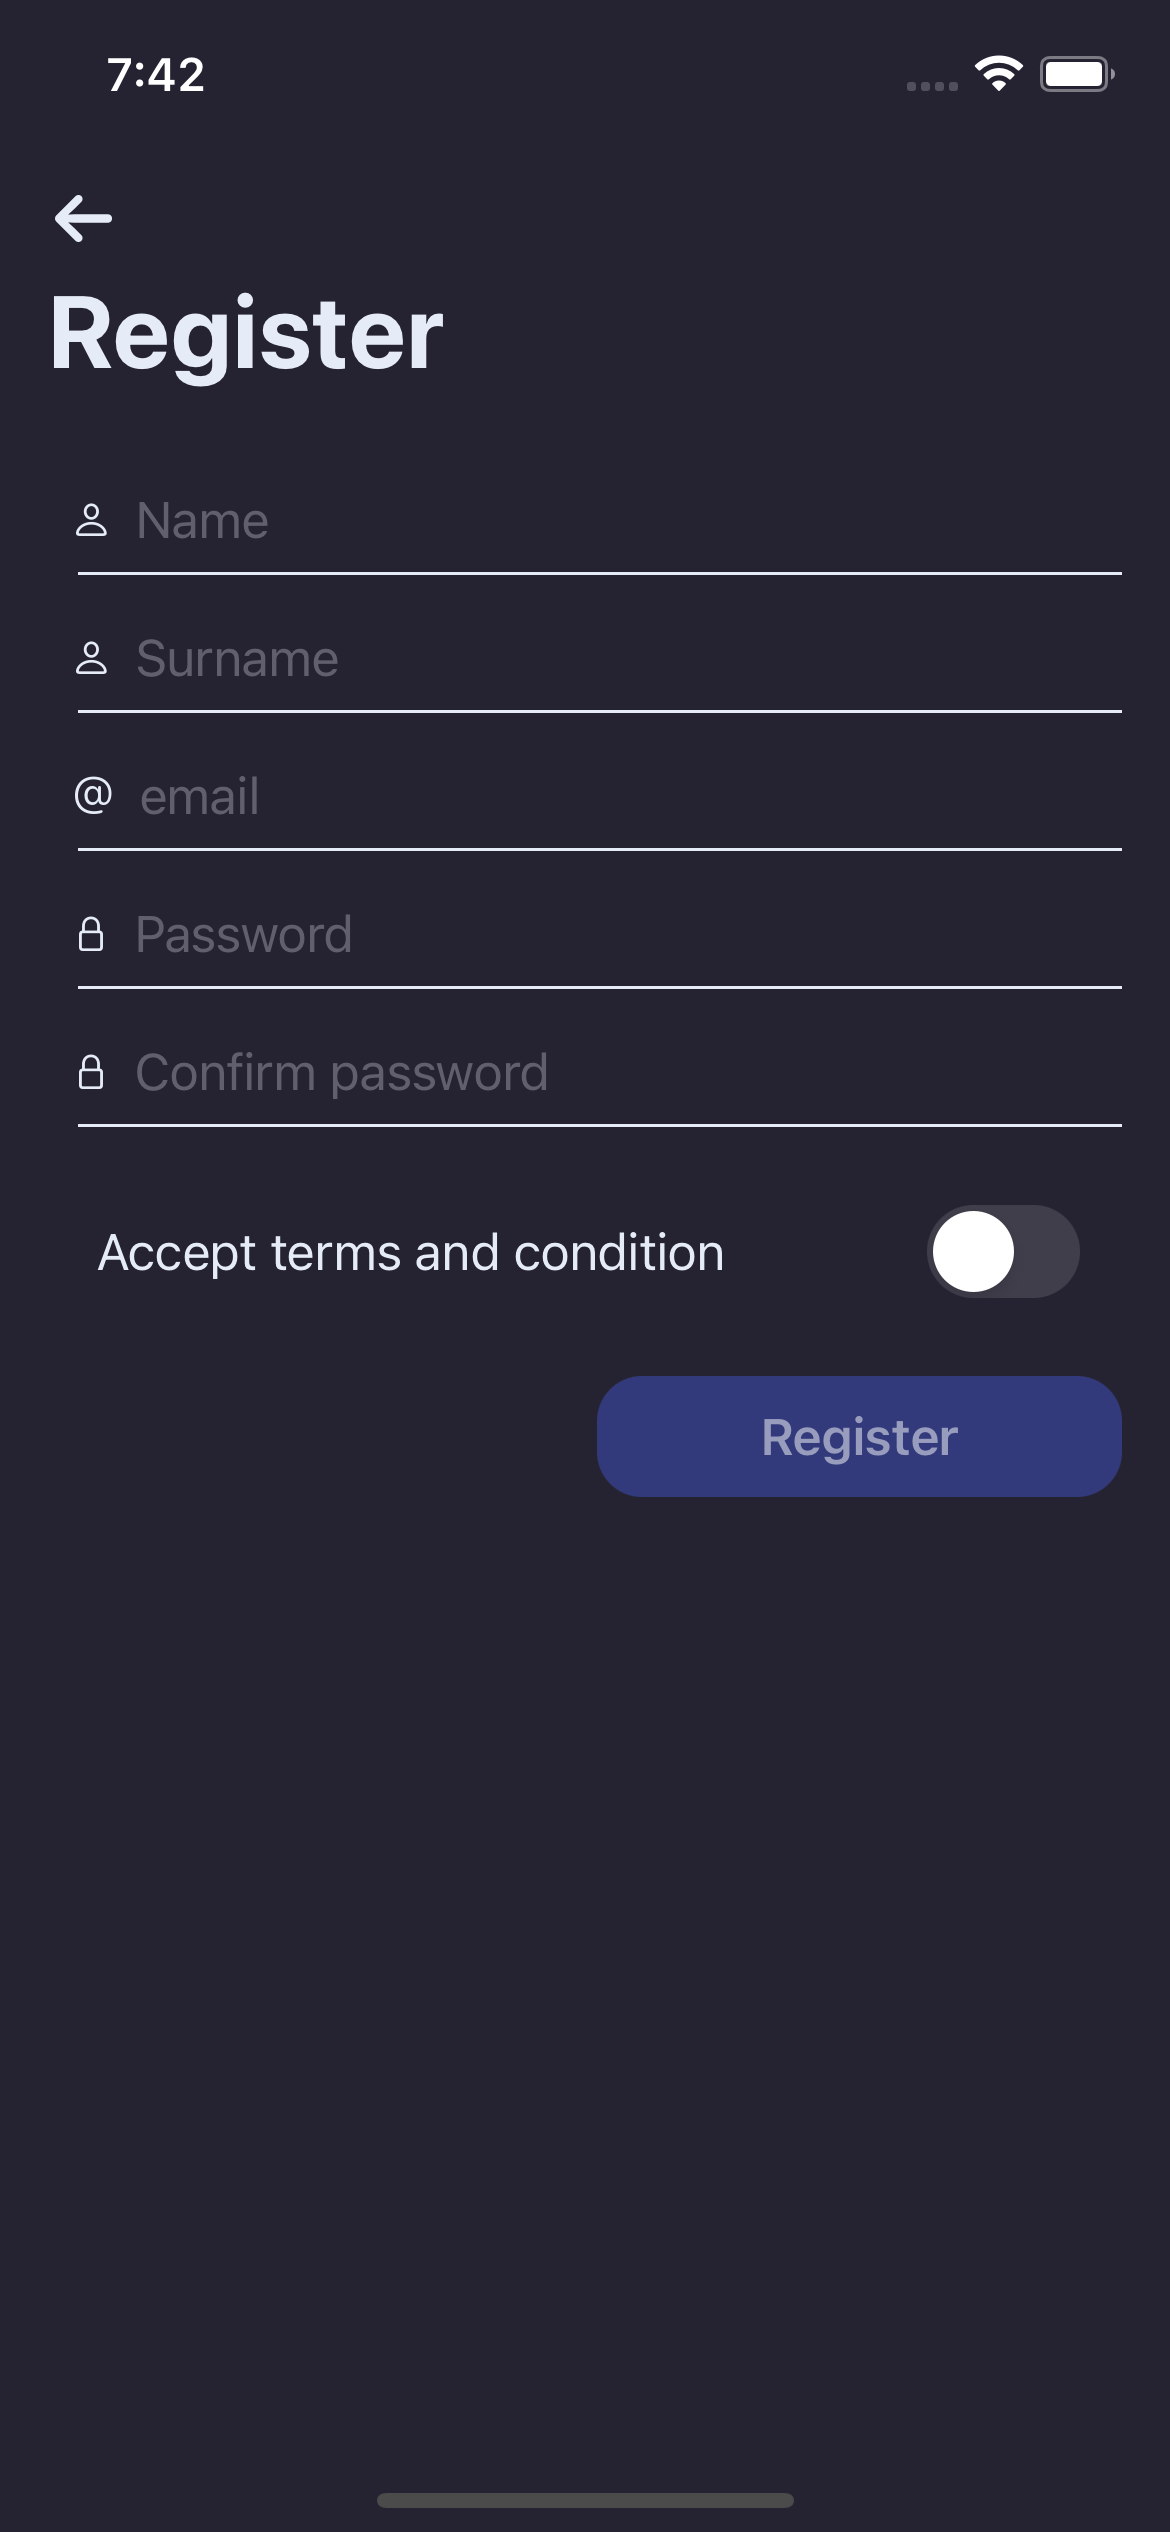
\includegraphics[scale=0.15]{images/interfaces/register_screen.png}
         \caption{Registration screen}
        \label{fig:register_screen}
\end{figure}
\FloatBarrier
This is the register view (fig: \ref{fig:register_screen}). The user can register an account by filling all the requirement parameters, accepting the terms and condition and clicking on register.

\begin{figure}[h!]
        \centering
        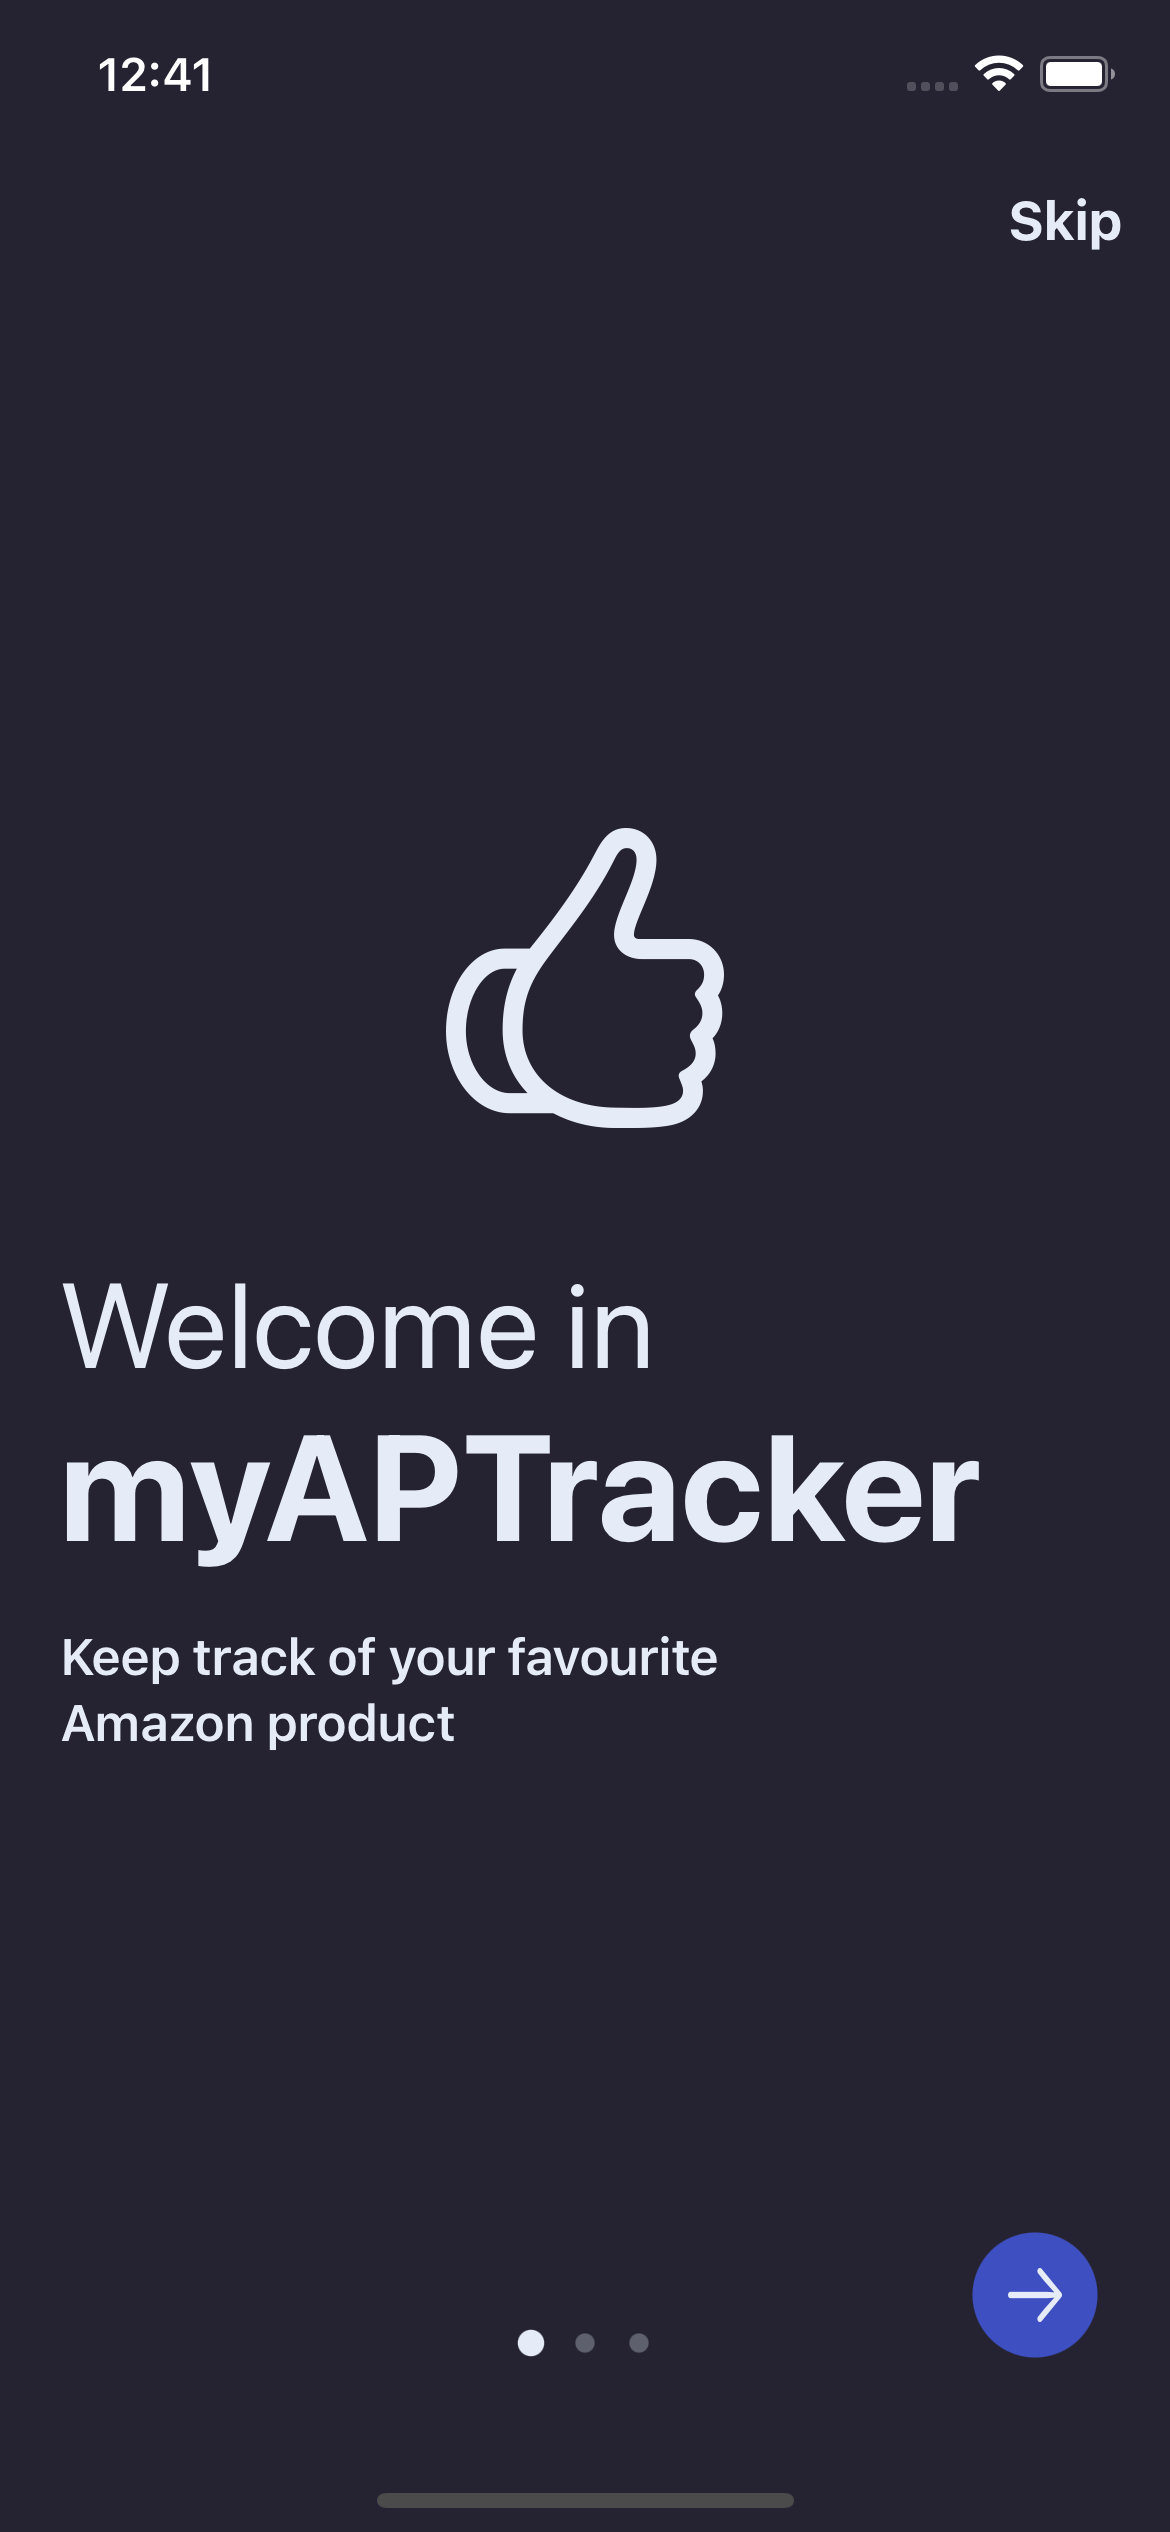
\includegraphics[scale=0.15]{images/interfaces/tutorial_screen_1.png}
        \caption{First screen of the tutorial}
        \label{fig:tutorial_screen_1}
\end{figure}
\FloatBarrier
This is the first page of the tutorial (fig: \ref{fig:tutorial_screen_1}). This view welcomes the user in the application. From here the user can continue the tutorial or skip it.

\begin{figure}[h!]
        \centering
        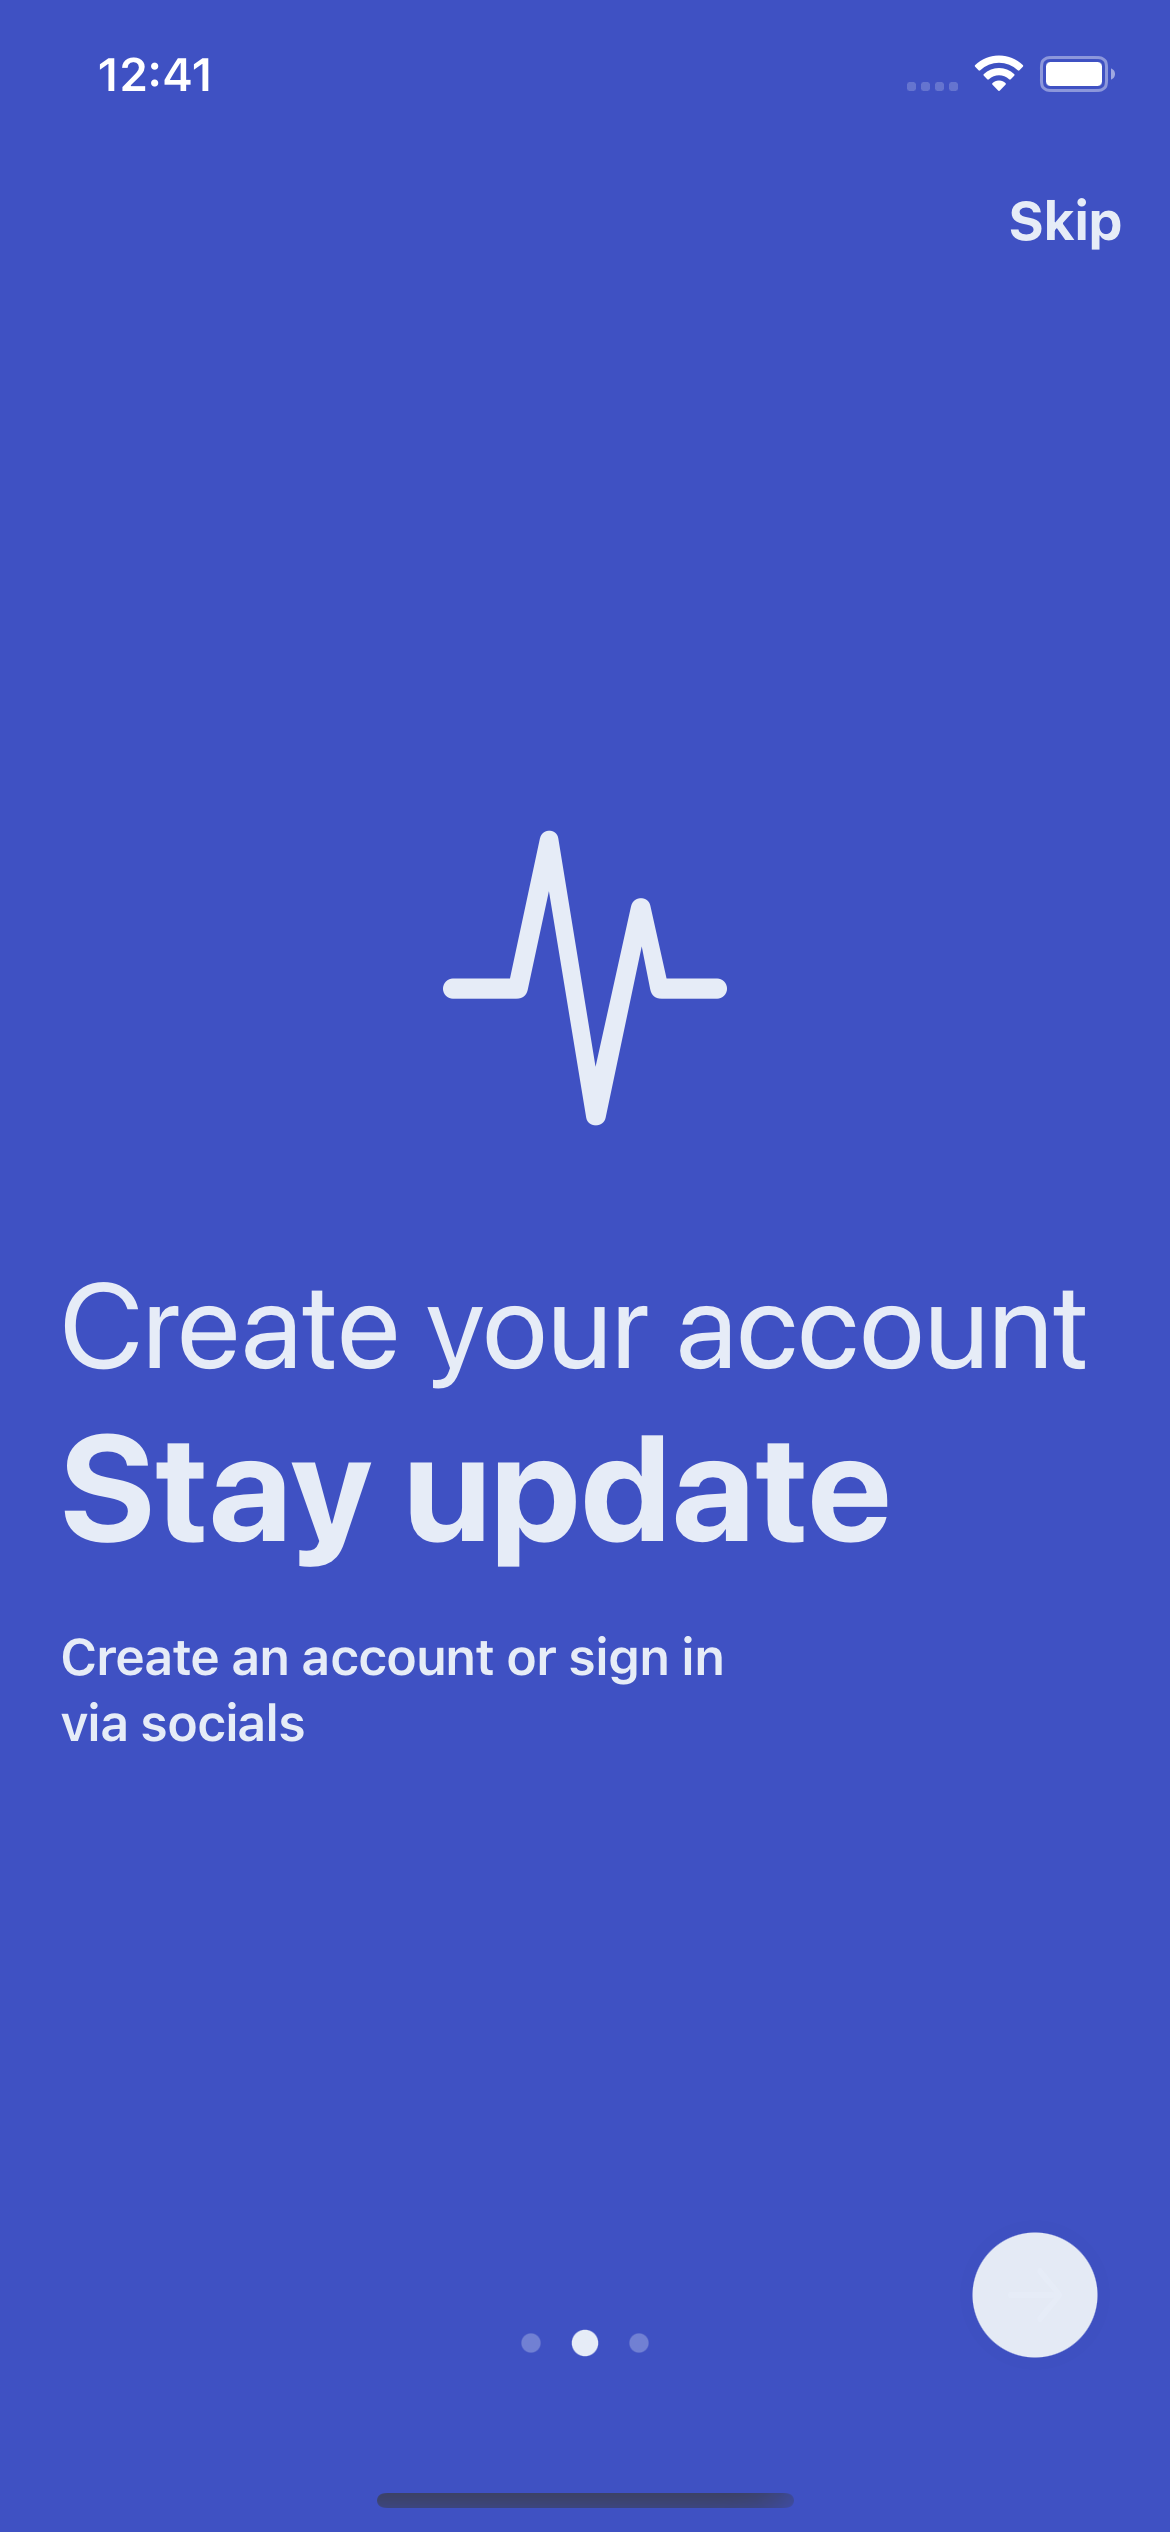
\includegraphics[scale=0.15]{images/interfaces/tutorial_screen_2.png}
        \caption{Second screen of the tutorial}
        \label{fig:tutorial_screen_2}
\end{figure}
\FloatBarrier
This is the second page of the tutorial (fig: \ref{fig:tutorial_screen_2}). This view invite the user to log in in order to have full access to the application. From here the user can continue the tutorial or skip it.

\begin{figure}[h!]
        \centering
        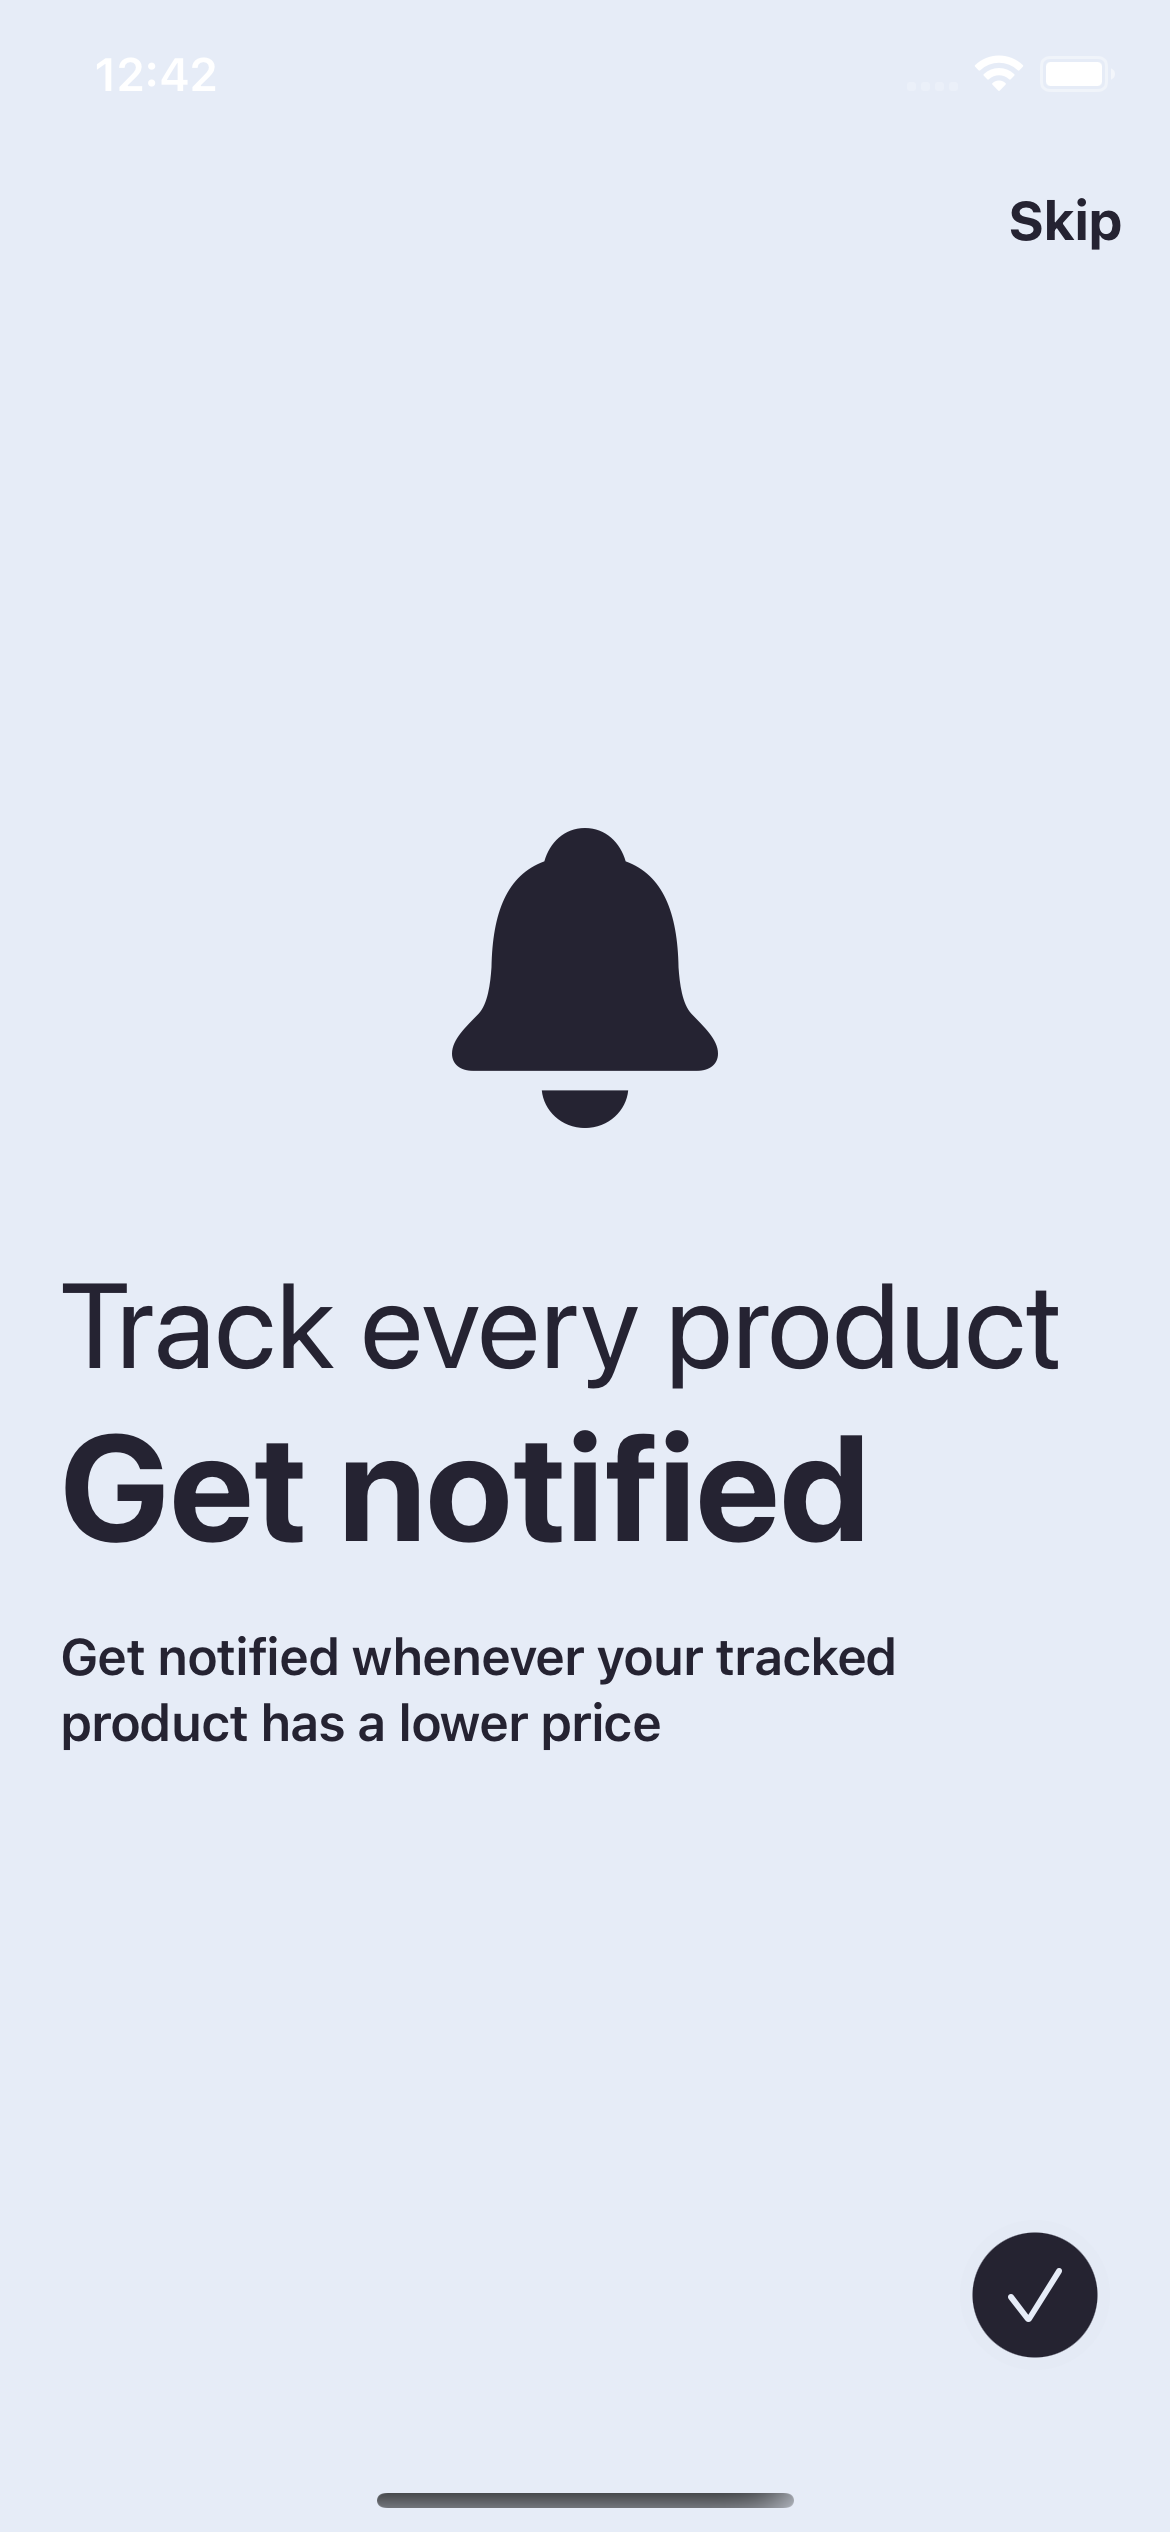
\includegraphics[scale=0.15]{images/interfaces/tutorial_screen_3.png}
        \caption{Third screen of the tutorial}
        \label{fig:tutorial_screen_3}
\end{figure}
\FloatBarrier
This is the last page of the tutorial (fig: \ref{fig:tutorial_screen_3}). This view invites the user to turn on the notification, because the application will notify the user when some products become available below the threshold set by the user. From here the user can exit from the tutorial.

\begin{figure}[h!]
        \centering
        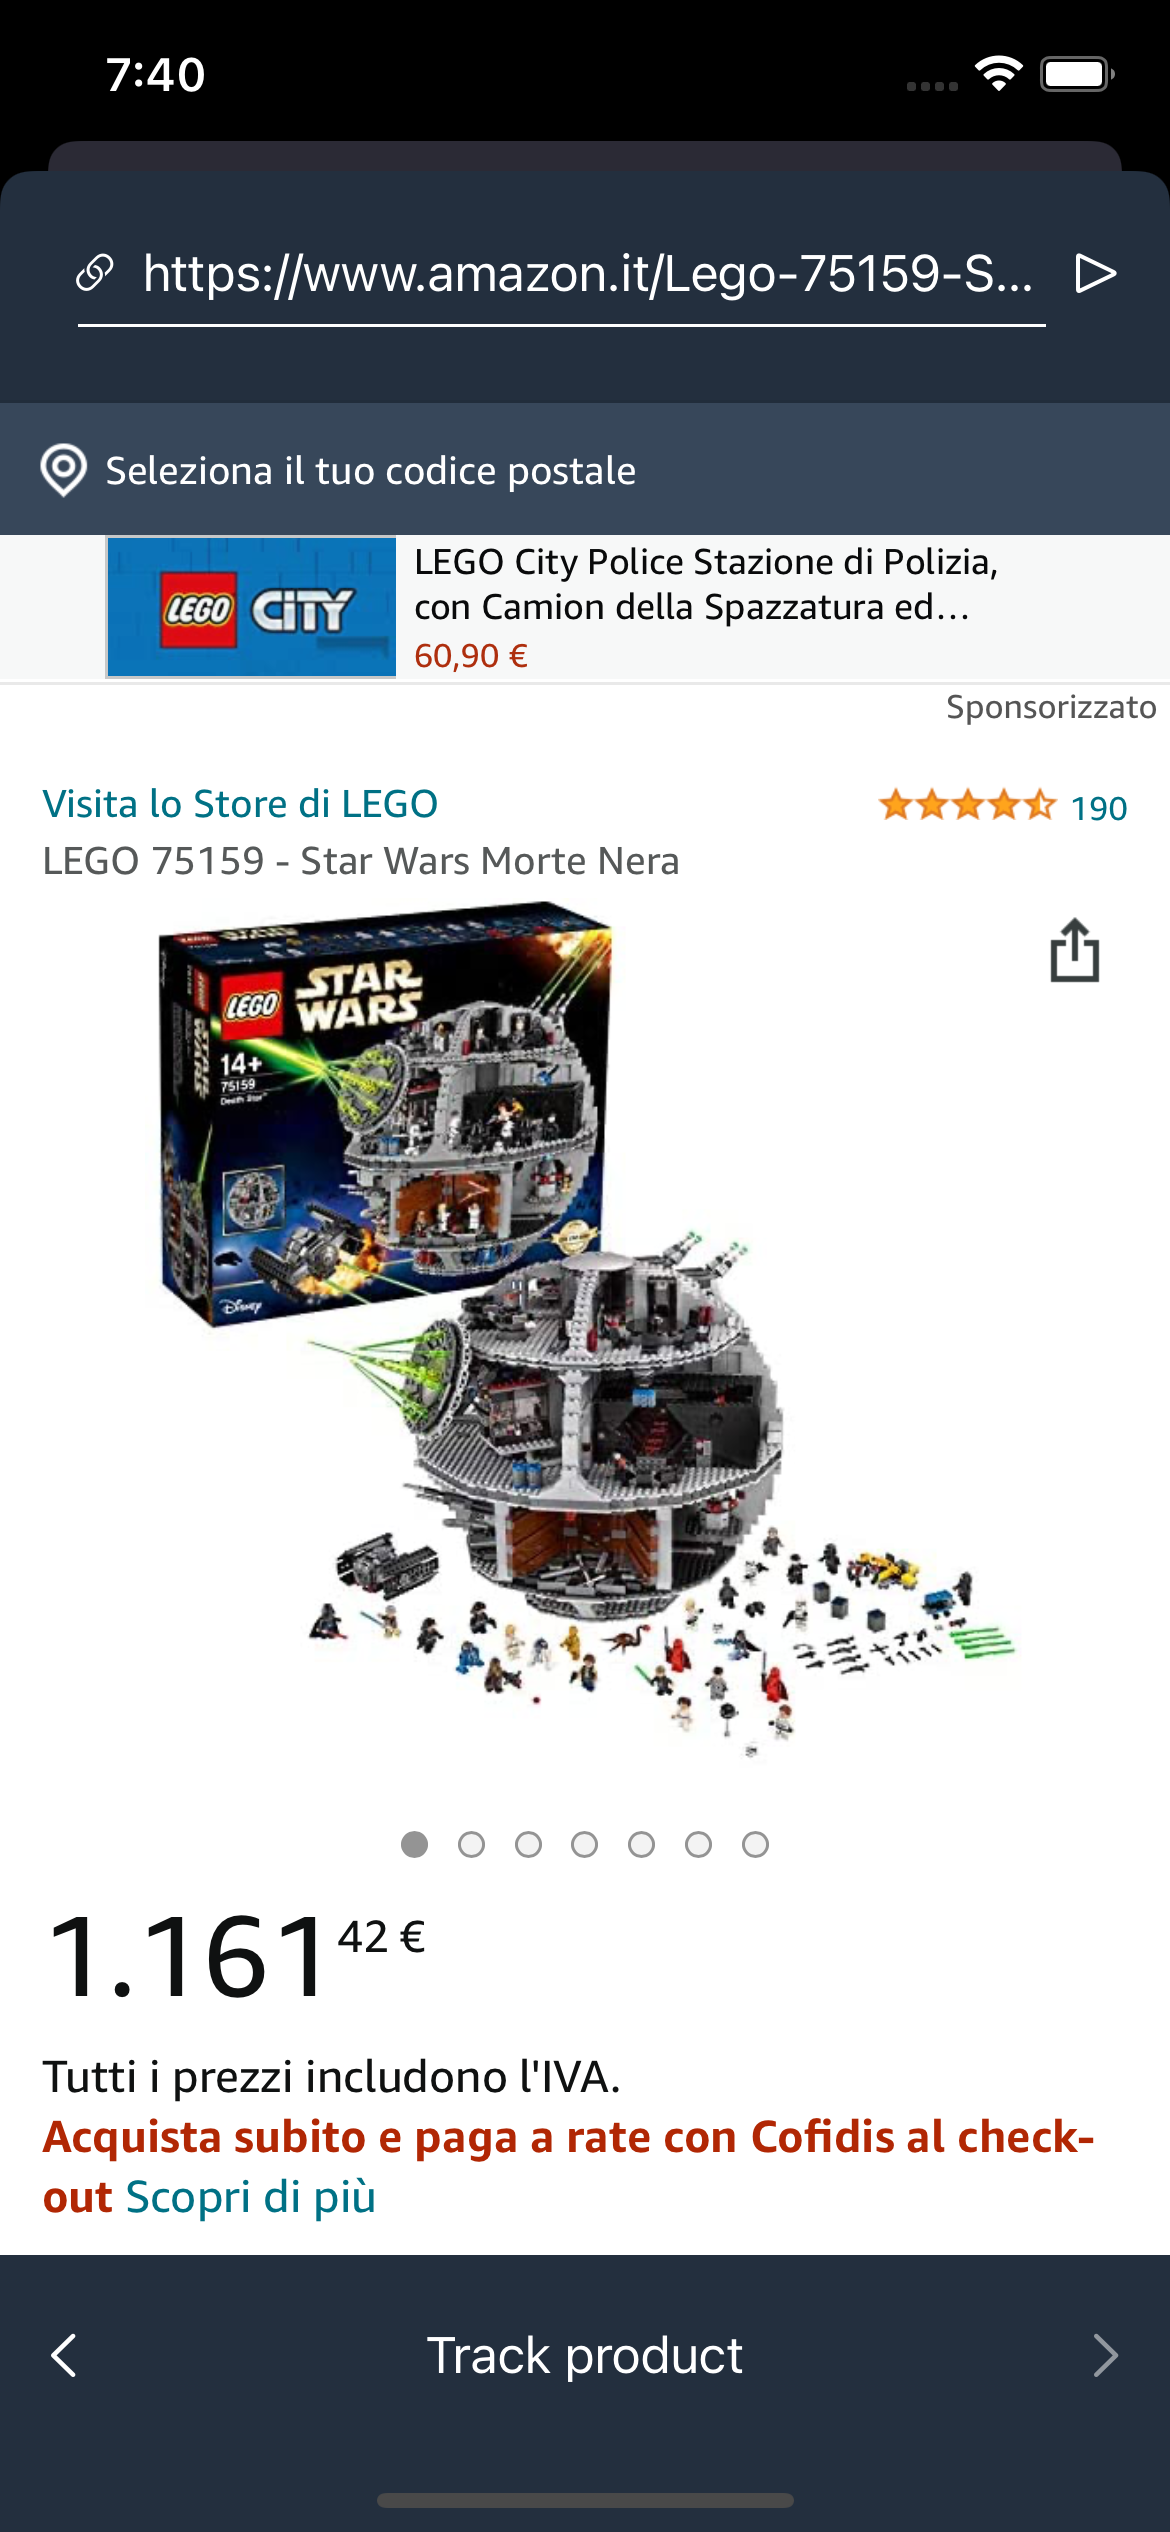
\includegraphics[scale=0.15]{images/interfaces/tracking_product_screen.png}
        \caption{User track a new product screen}
        \label{fig:tracking_product_screen}
\end{figure}
\FloatBarrier
This is the view where the user can start track a new product (fig: \ref{fig:tracking_product_screen}). It is a web browser configured on Amazon website with an handler to detect if the page is a product or other screens. For security reasons the user is not allowed to leave amazon website.\\
The Amazon browser in accessible by clicking in the "plus" button from the main view which is a container with a tab bar to navigate between the 4 main screens (on iPhone) while on the iPad the same view is accessible from the application sidebar (see the end of the section).

\begin{figure}[h!]
        \centering
        \begin{subfigure}[b]{0.3\textwidth}
            \centering
            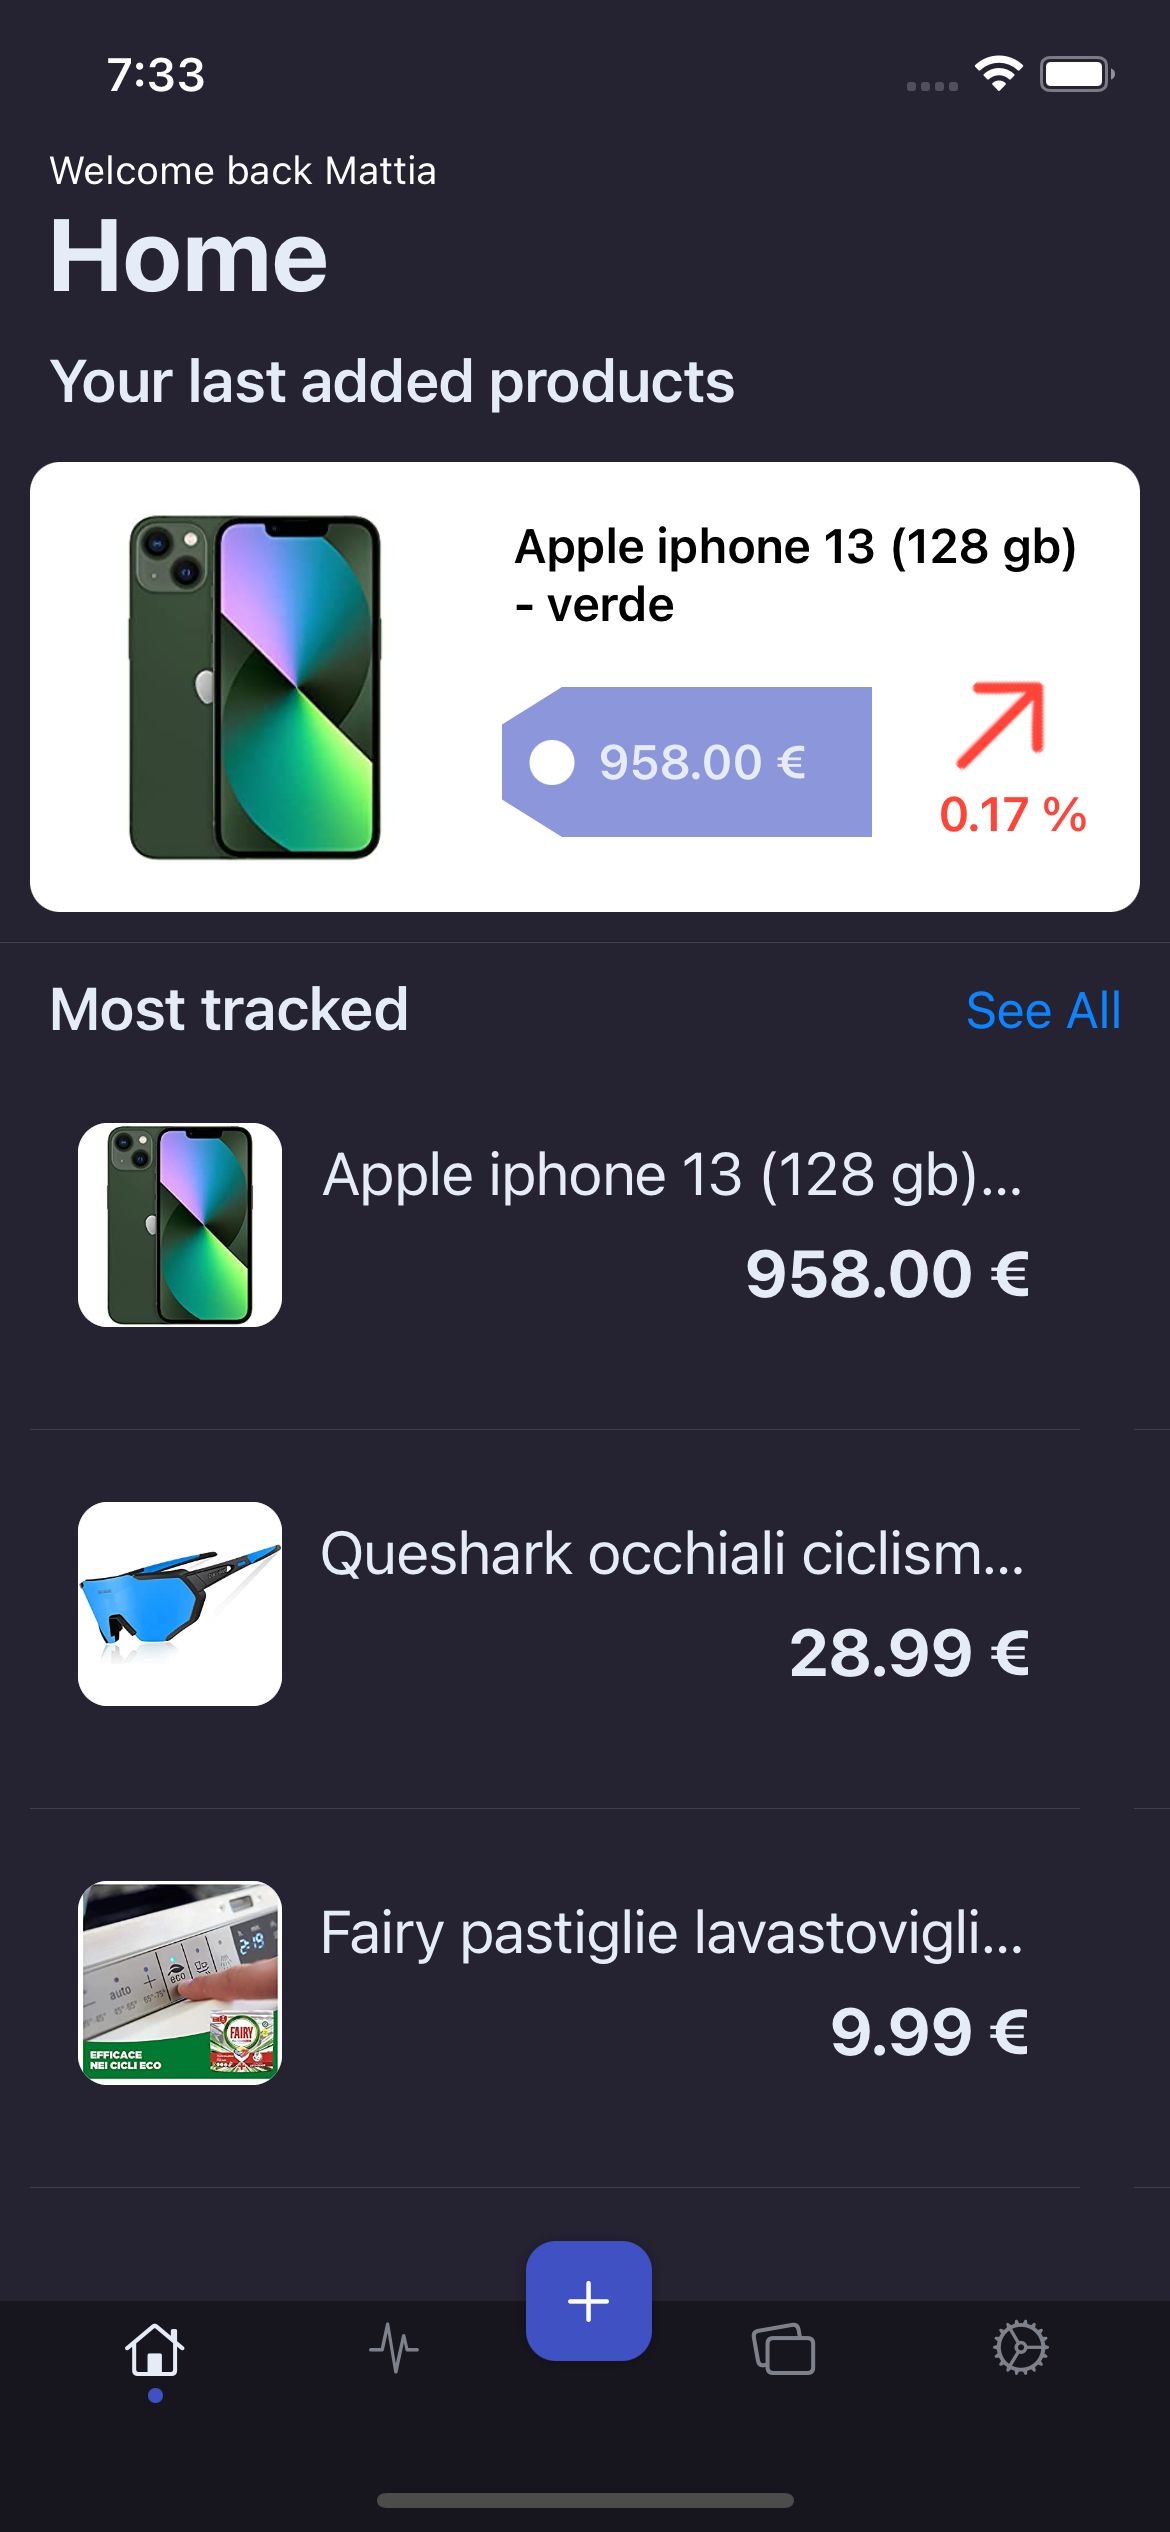
\includegraphics[width=\textwidth]{images/interfaces/home_screen.png}
            \caption{iPhone}
            \label{fig:home_screen_iphone}
        \end{subfigure}
        \begin{subfigure}[b]{0.45\textwidth}
            \centering
            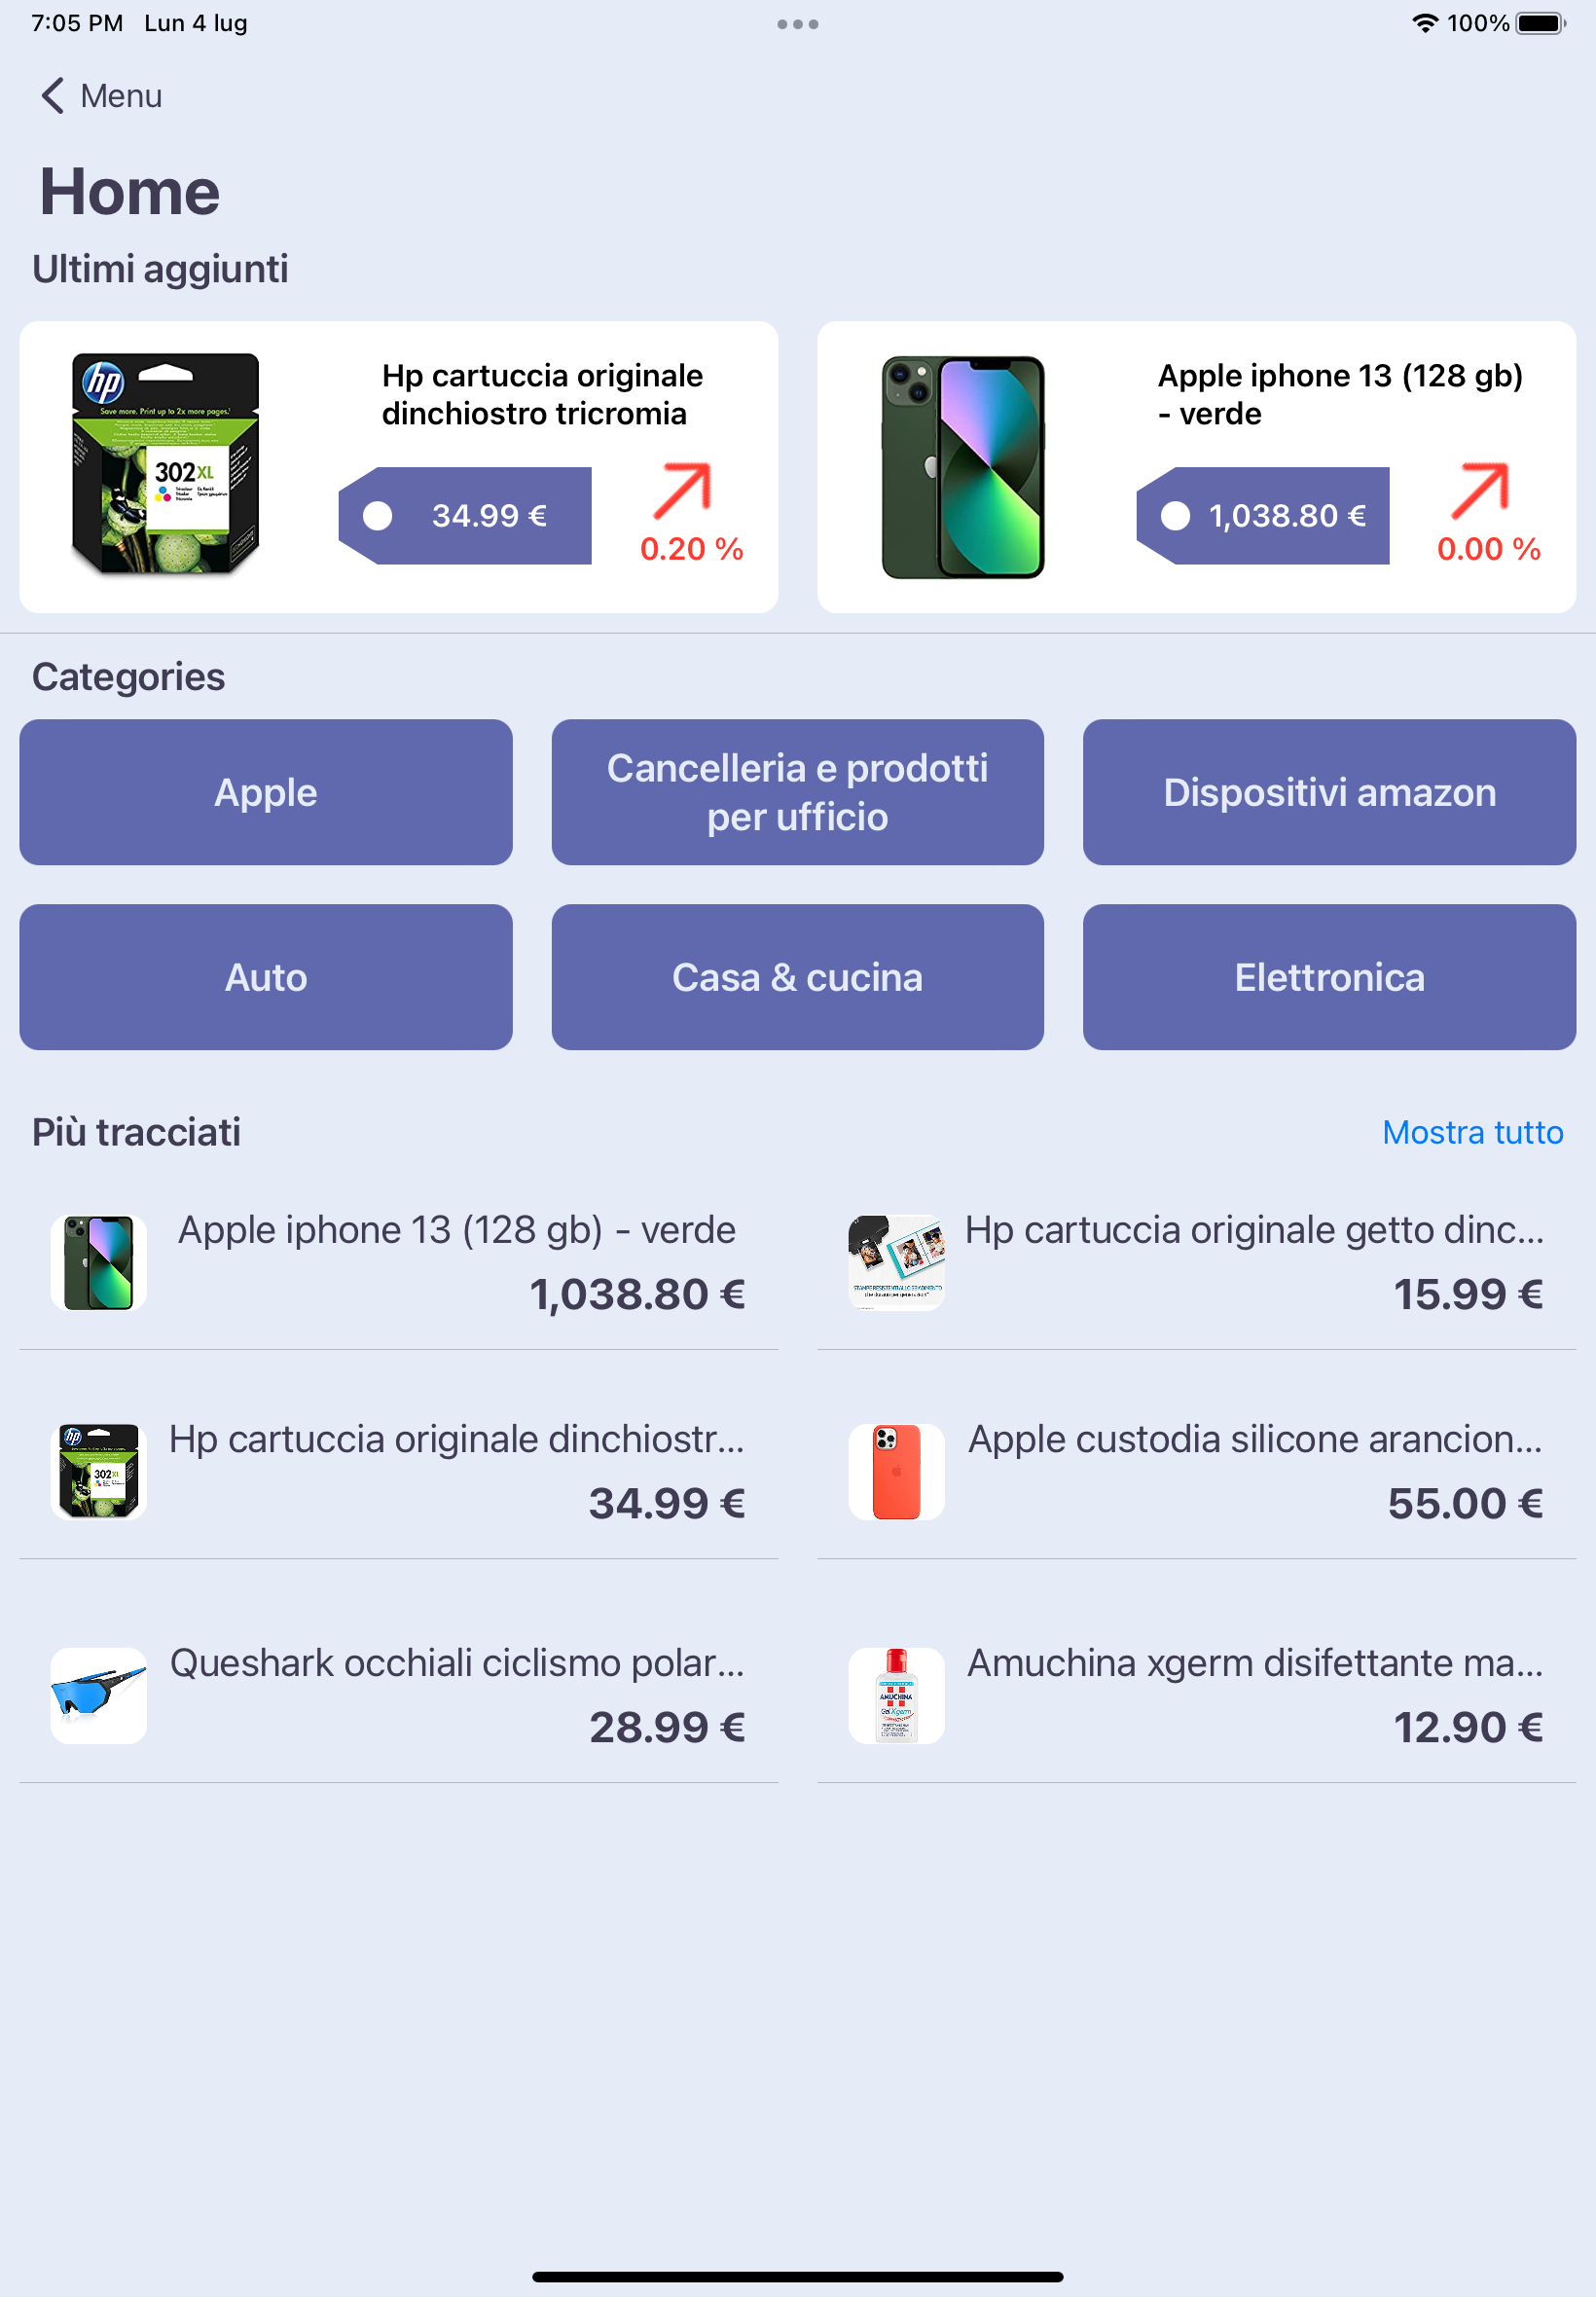
\includegraphics[width=\textwidth]{images/interfaces/home_screen_ipad.png}
            \caption{iPad}
            \label{fig:home_screen_ipad}
        \end{subfigure}
         \caption{Home screen}
        \label{fig:home_screen}
\end{figure}
\FloatBarrier
This is the home view (fig: \ref{fig:home_screen}) which is shown when the app finish launching. From here the user can scroll his last tracked product on the top or he can also navigate through the most tracked products. In addition, in the iPad interface, the user can also view a shortcut to access categories.

\begin{figure}[h!]
        \centering
        \begin{subfigure}[b]{0.3\textwidth}
            \centering
            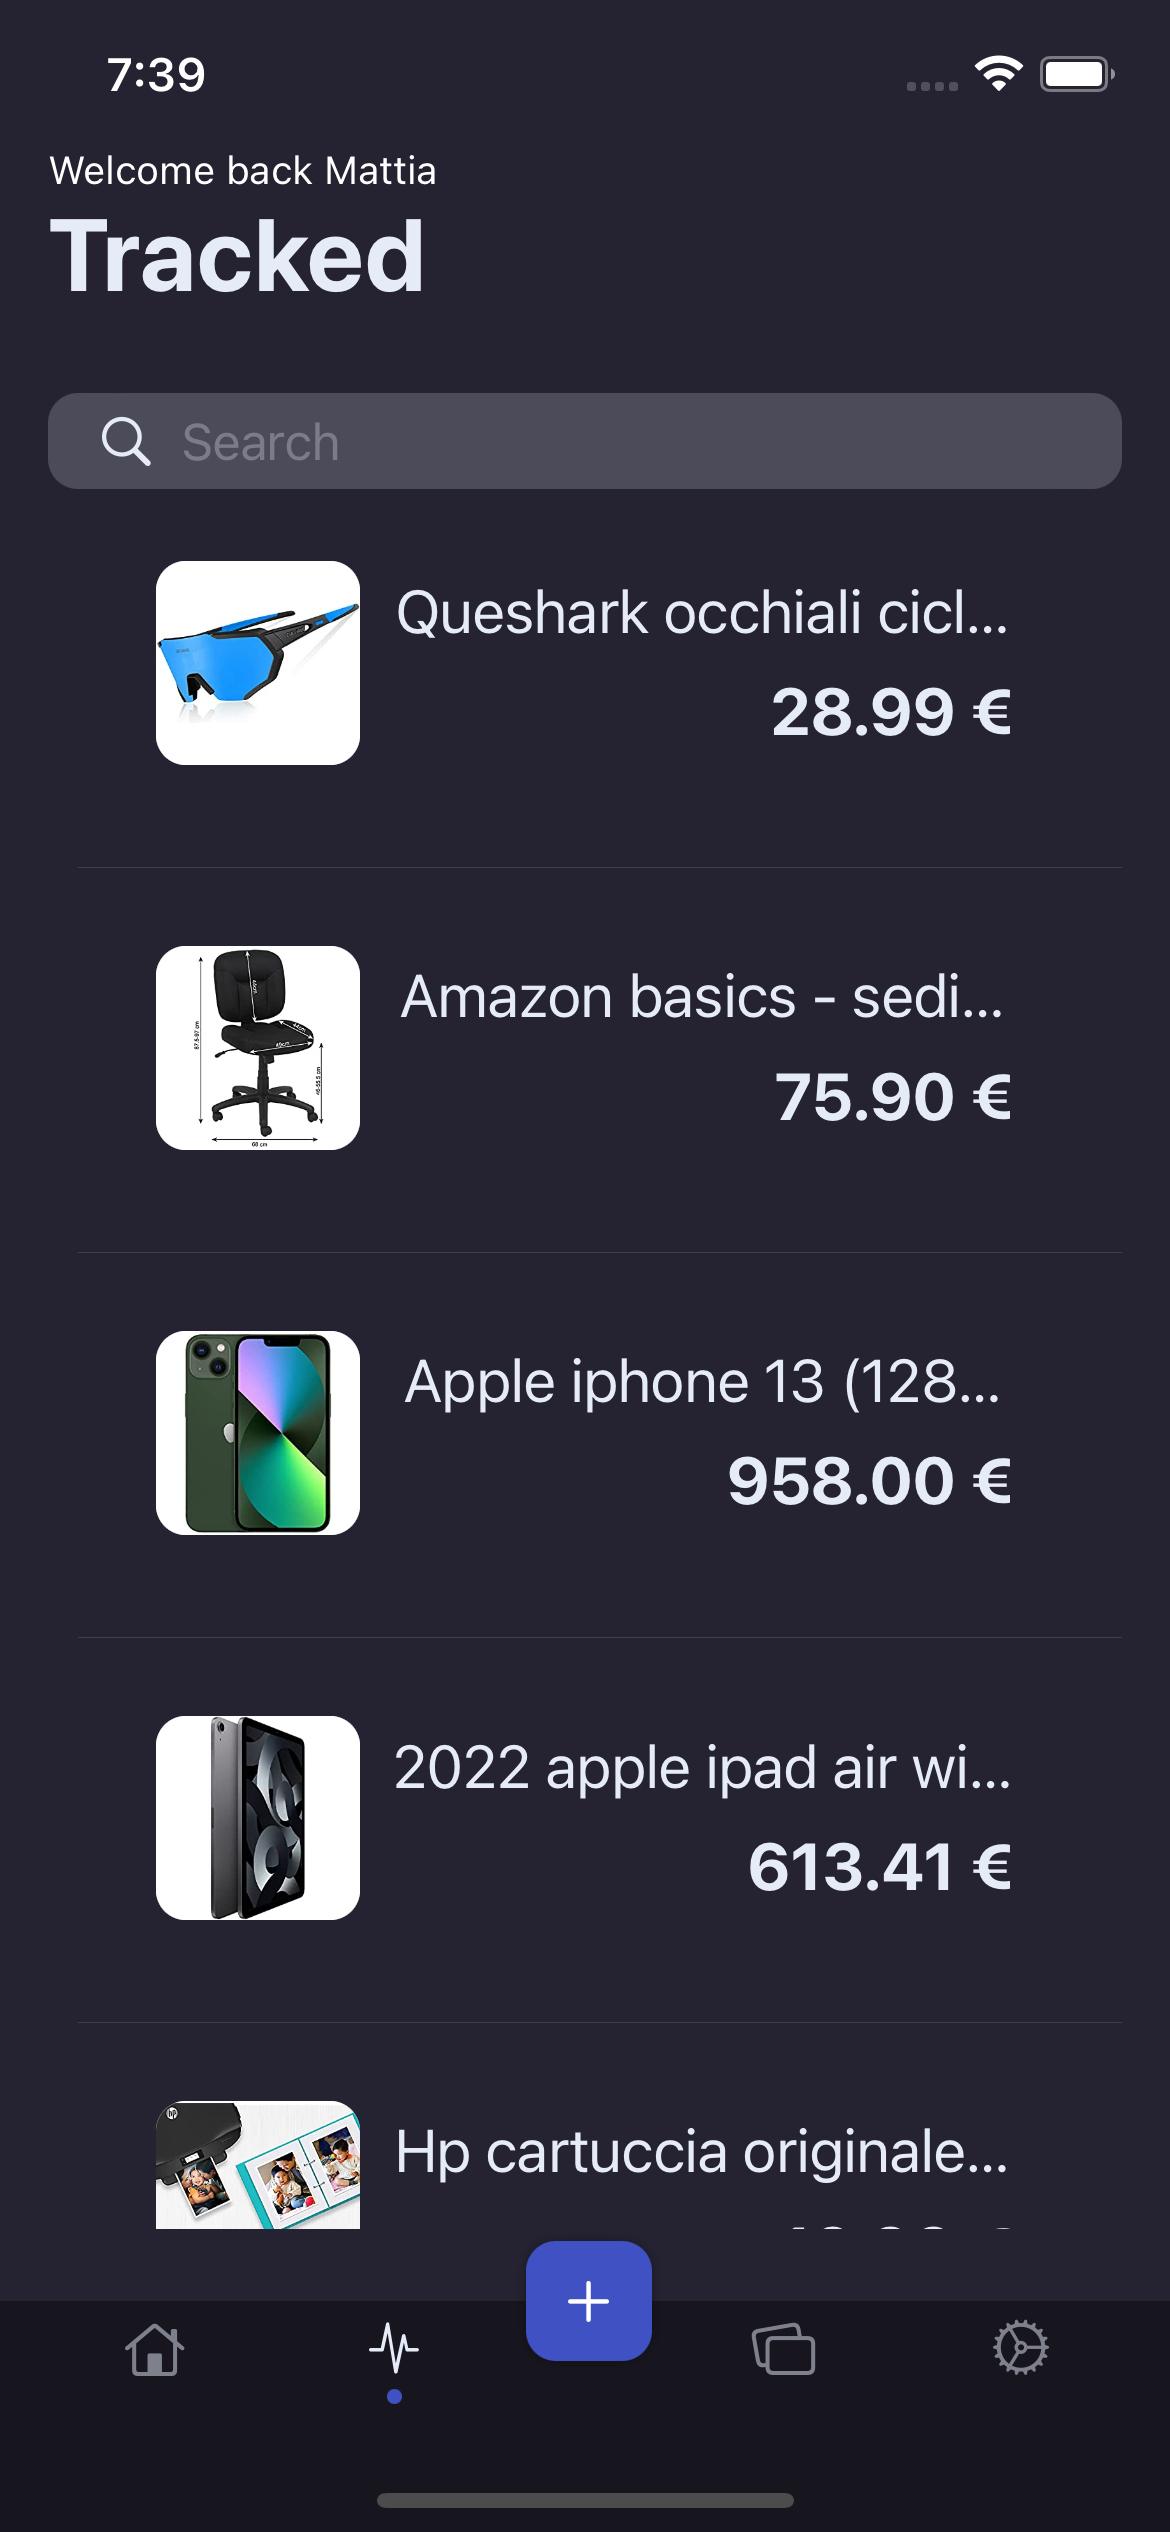
\includegraphics[width=\textwidth]{images/interfaces/user_tracked_screen.png}
            \caption{iPhone}
            \label{fig:user_tracked_screen_iphone}
        \end{subfigure}
        \begin{subfigure}[b]{0.45\textwidth}
            \centering
            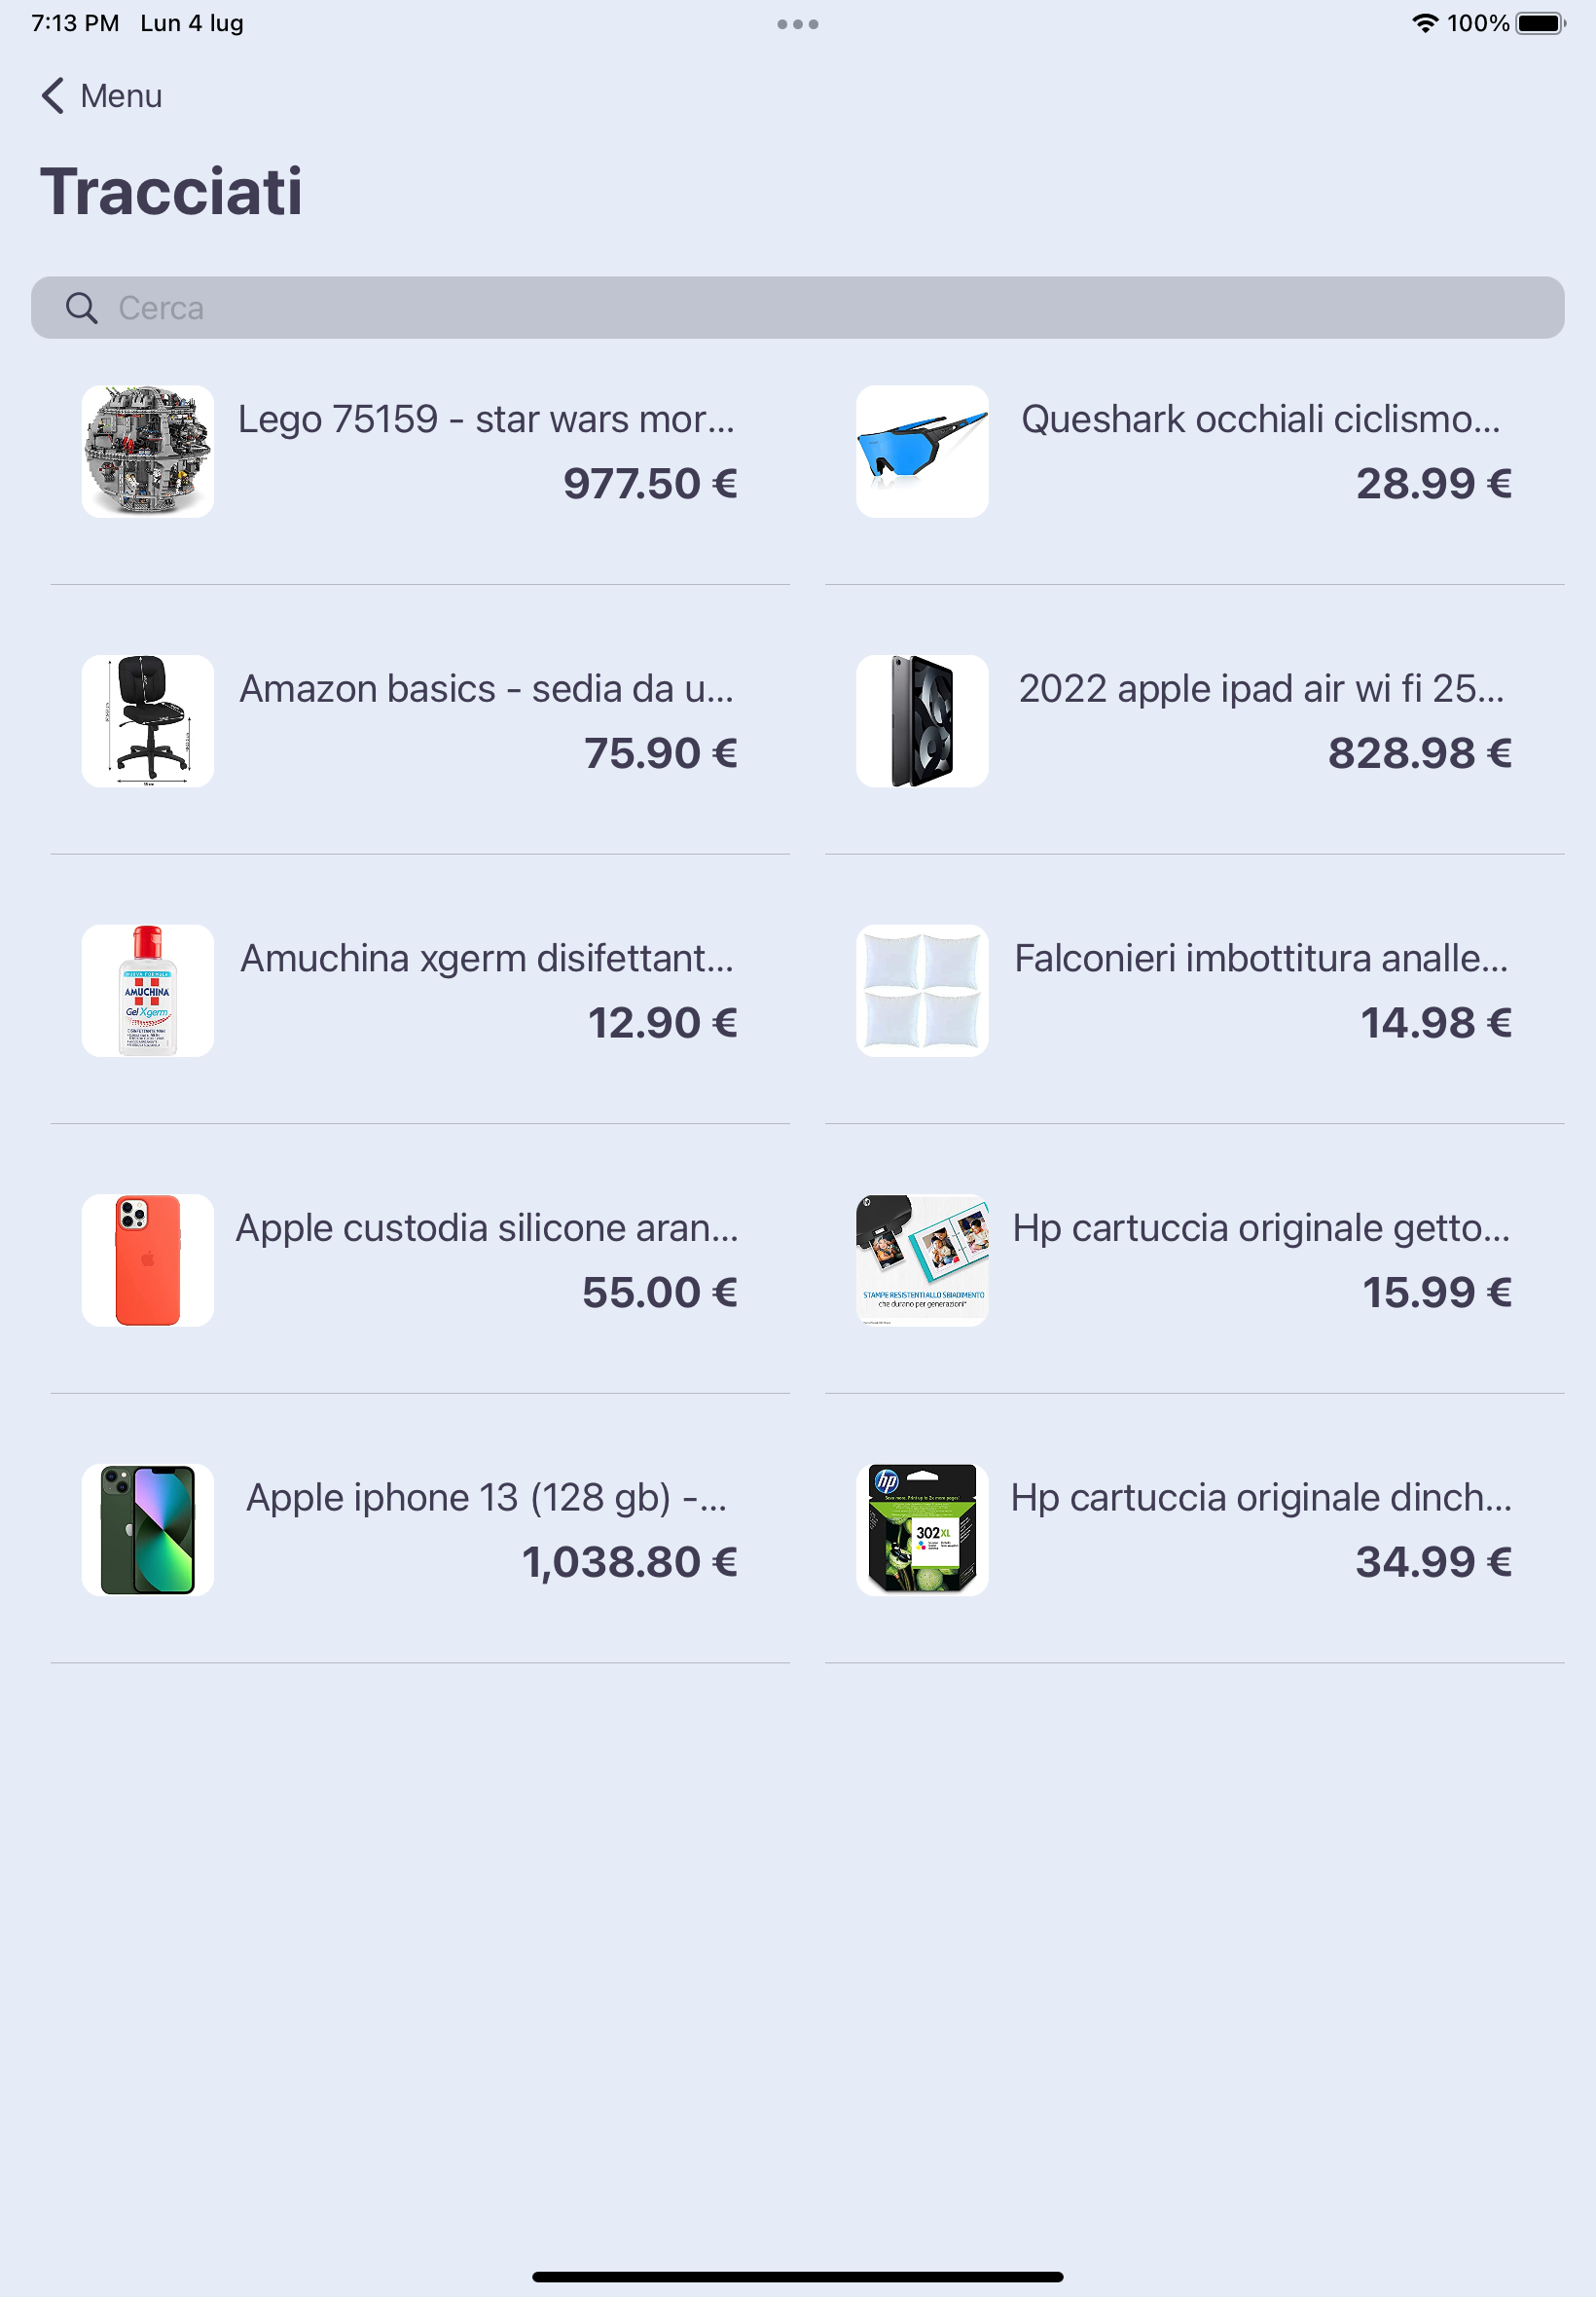
\includegraphics[width=\textwidth]{images/interfaces/user_tracked_screen_ipad.png}
            \caption{iPad}
            \label{fig:user_tracked_screen_ipad}
        \end{subfigure}
         \caption{User tracked products screen}
        \label{fig:user_tracked_screen}
\end{figure}
\FloatBarrier
This is the tracked product view accessible only  when a user is logged (fig: \ref{fig:user_tracked_screen}). From here the user can vertically scroll all his tracked products or can directly search for a specific product, using the search bar.

\begin{figure}[h!]
        \centering
        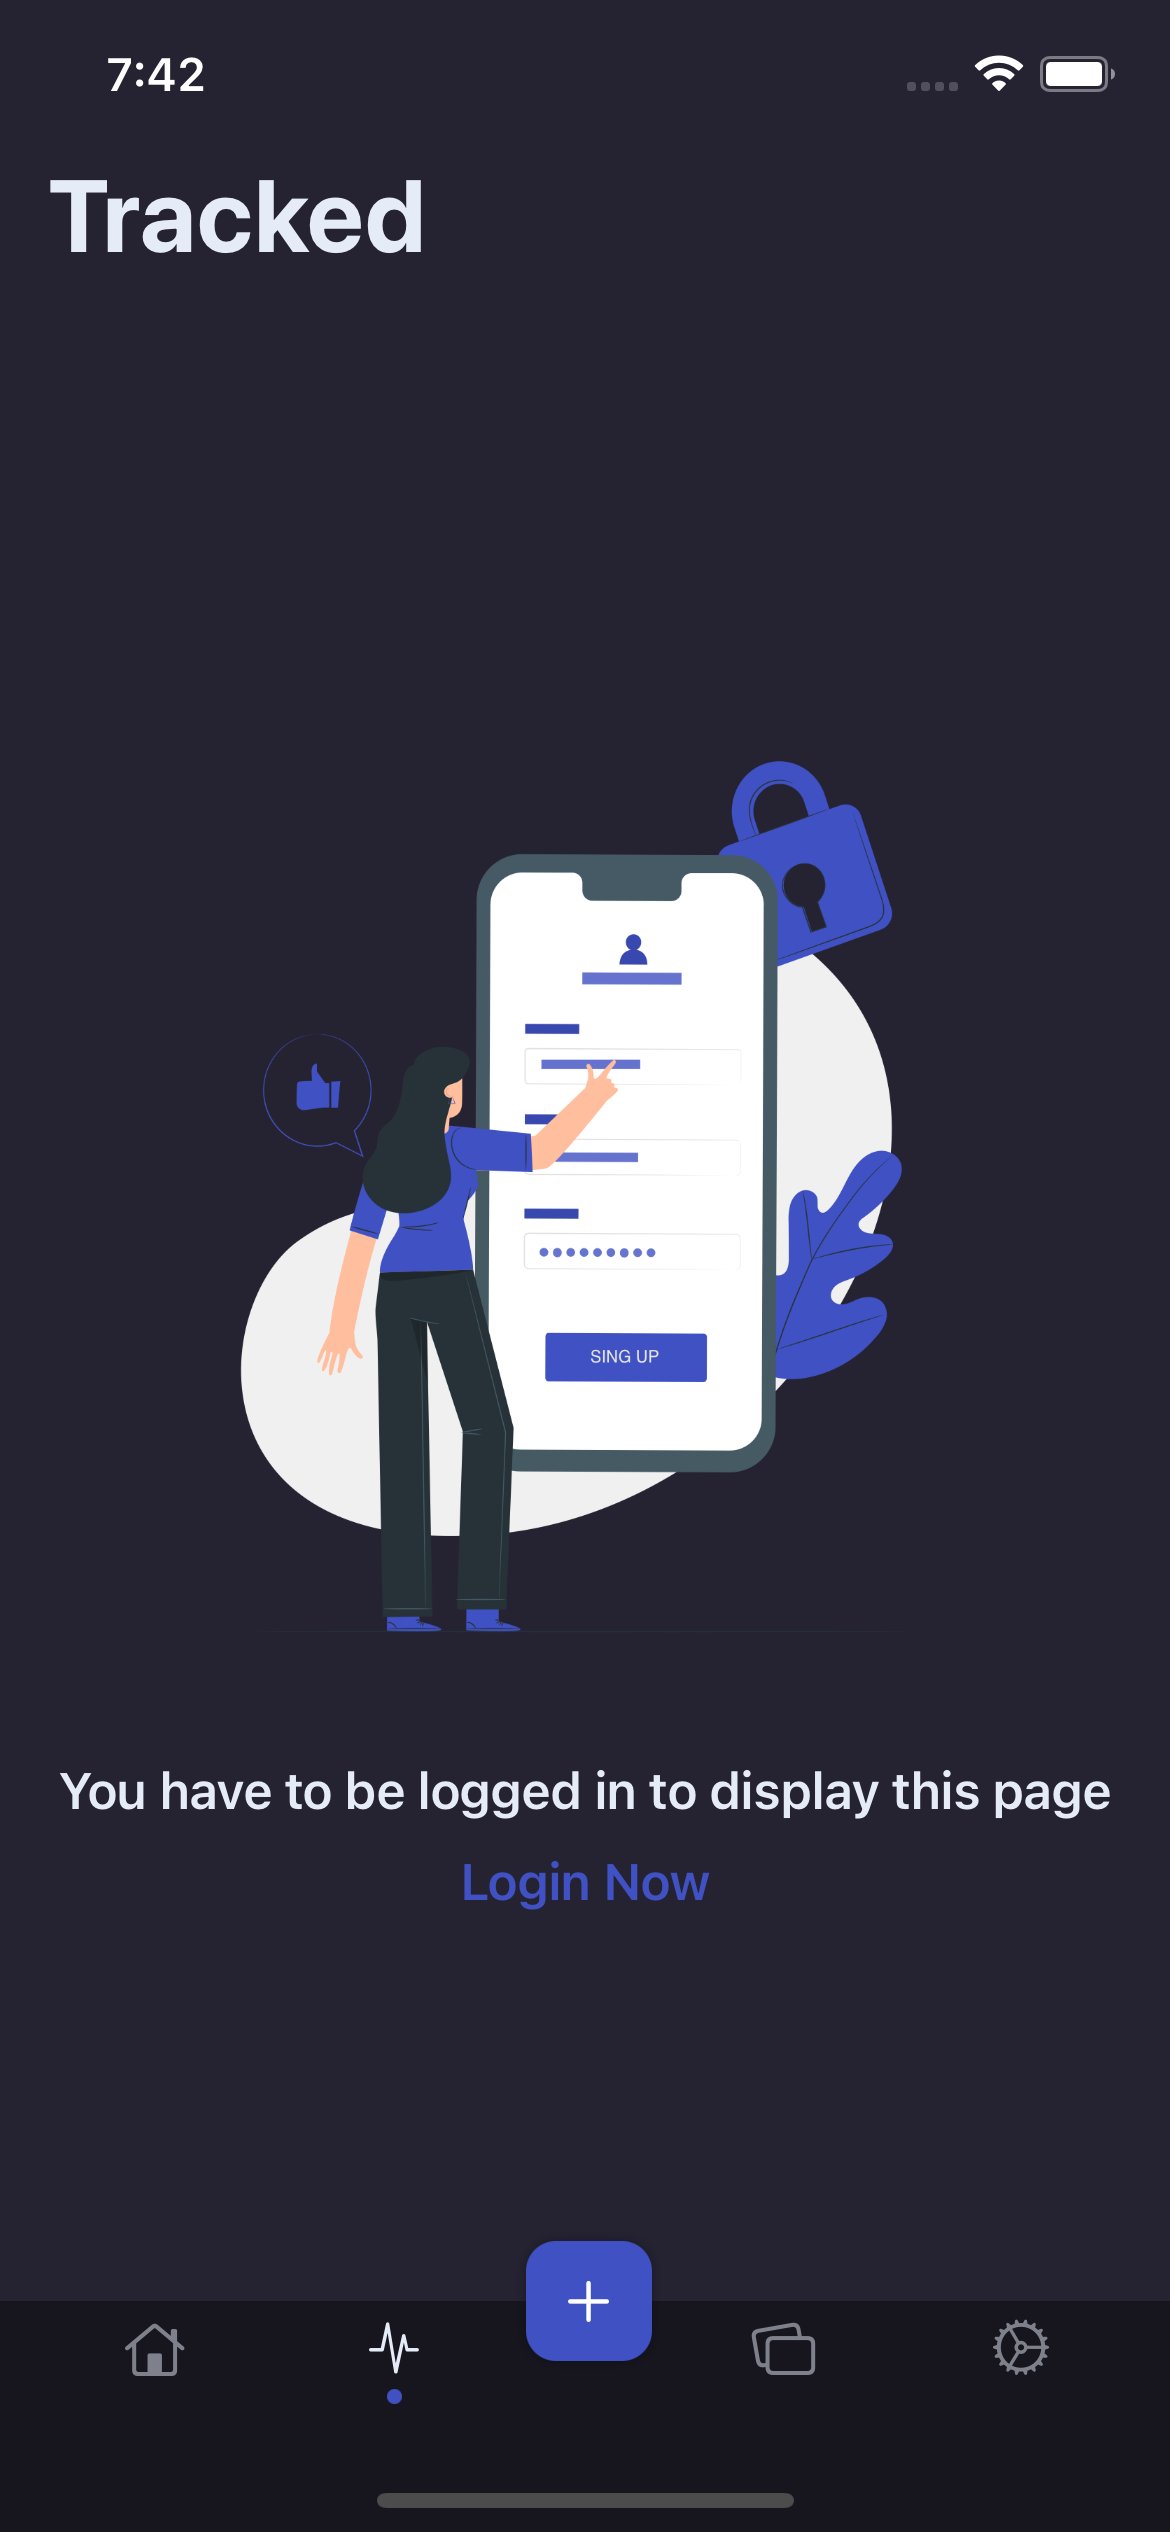
\includegraphics[scale=0.15]{images/interfaces/user_tracked_screen_not_logged.png}
        \caption{User tracked products screen, if user is not logged}
        \label{fig:user_tracked_screen_not_logged}
\end{figure}
\FloatBarrier
This is the tracked product view when a user is not logged (fig: \ref{fig:user_tracked_screen_not_logged}). Since the user can track product only if it is registered, this view is useless if the user is not logged, so it is only present a suggestion to invite the user to login.

\begin{figure}[h!]
        \centering
        \begin{subfigure}[b]{0.3\textwidth}
            \centering
            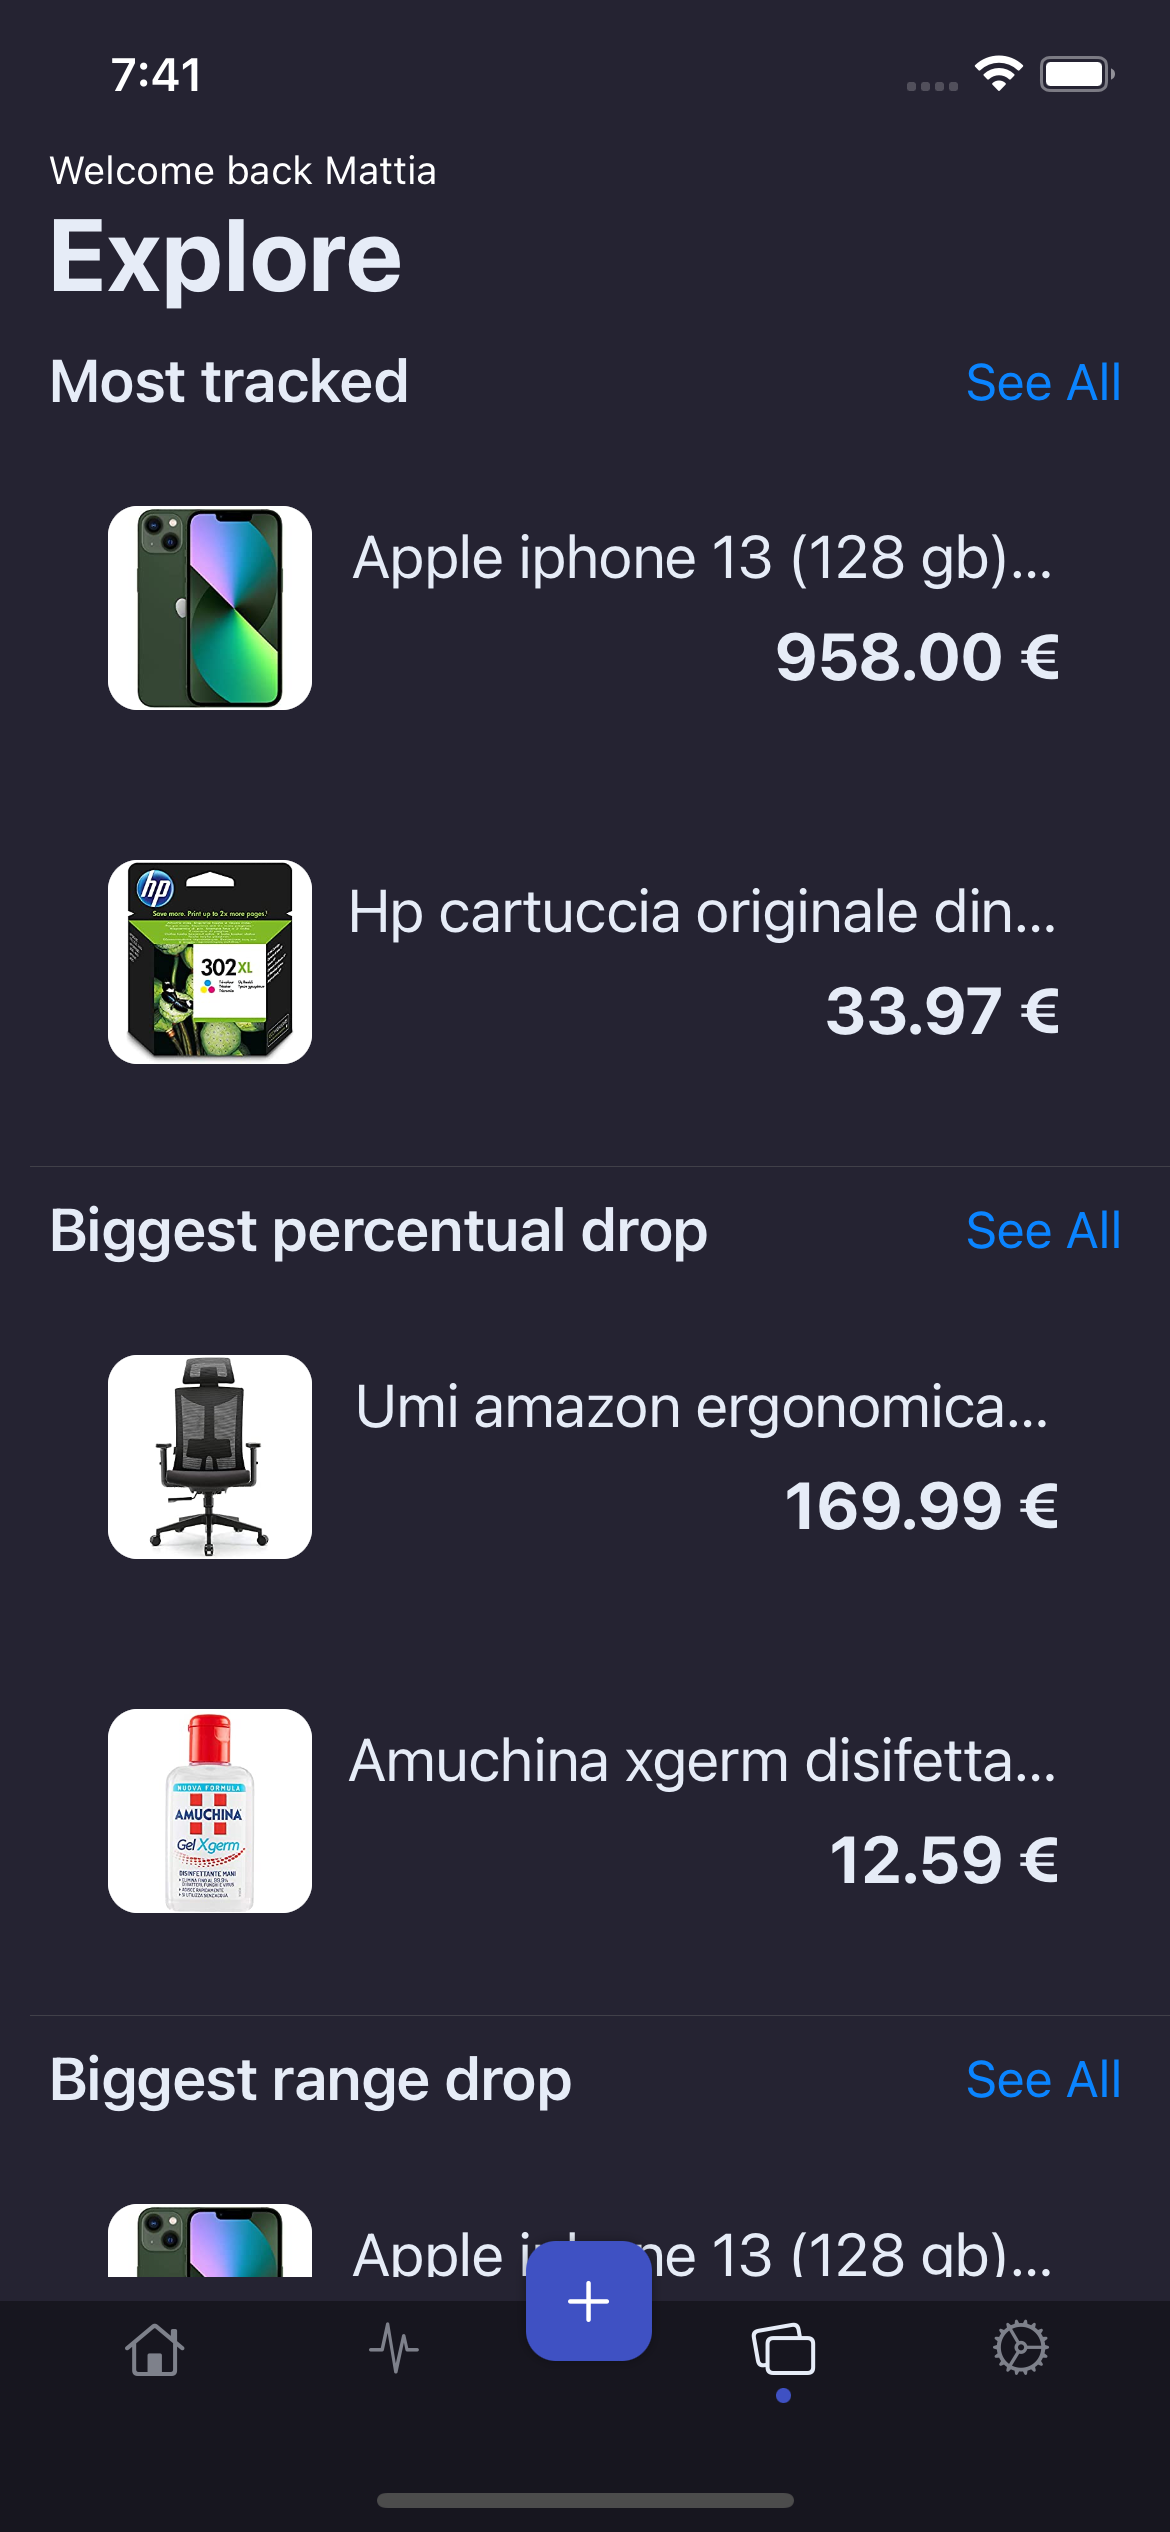
\includegraphics[width=\textwidth]{images/interfaces/explore_screen.png}
            \caption{iPhone}
            \label{fig:explore_screen_iphone}
        \end{subfigure}
        \begin{subfigure}[b]{0.45\textwidth}
            \centering
            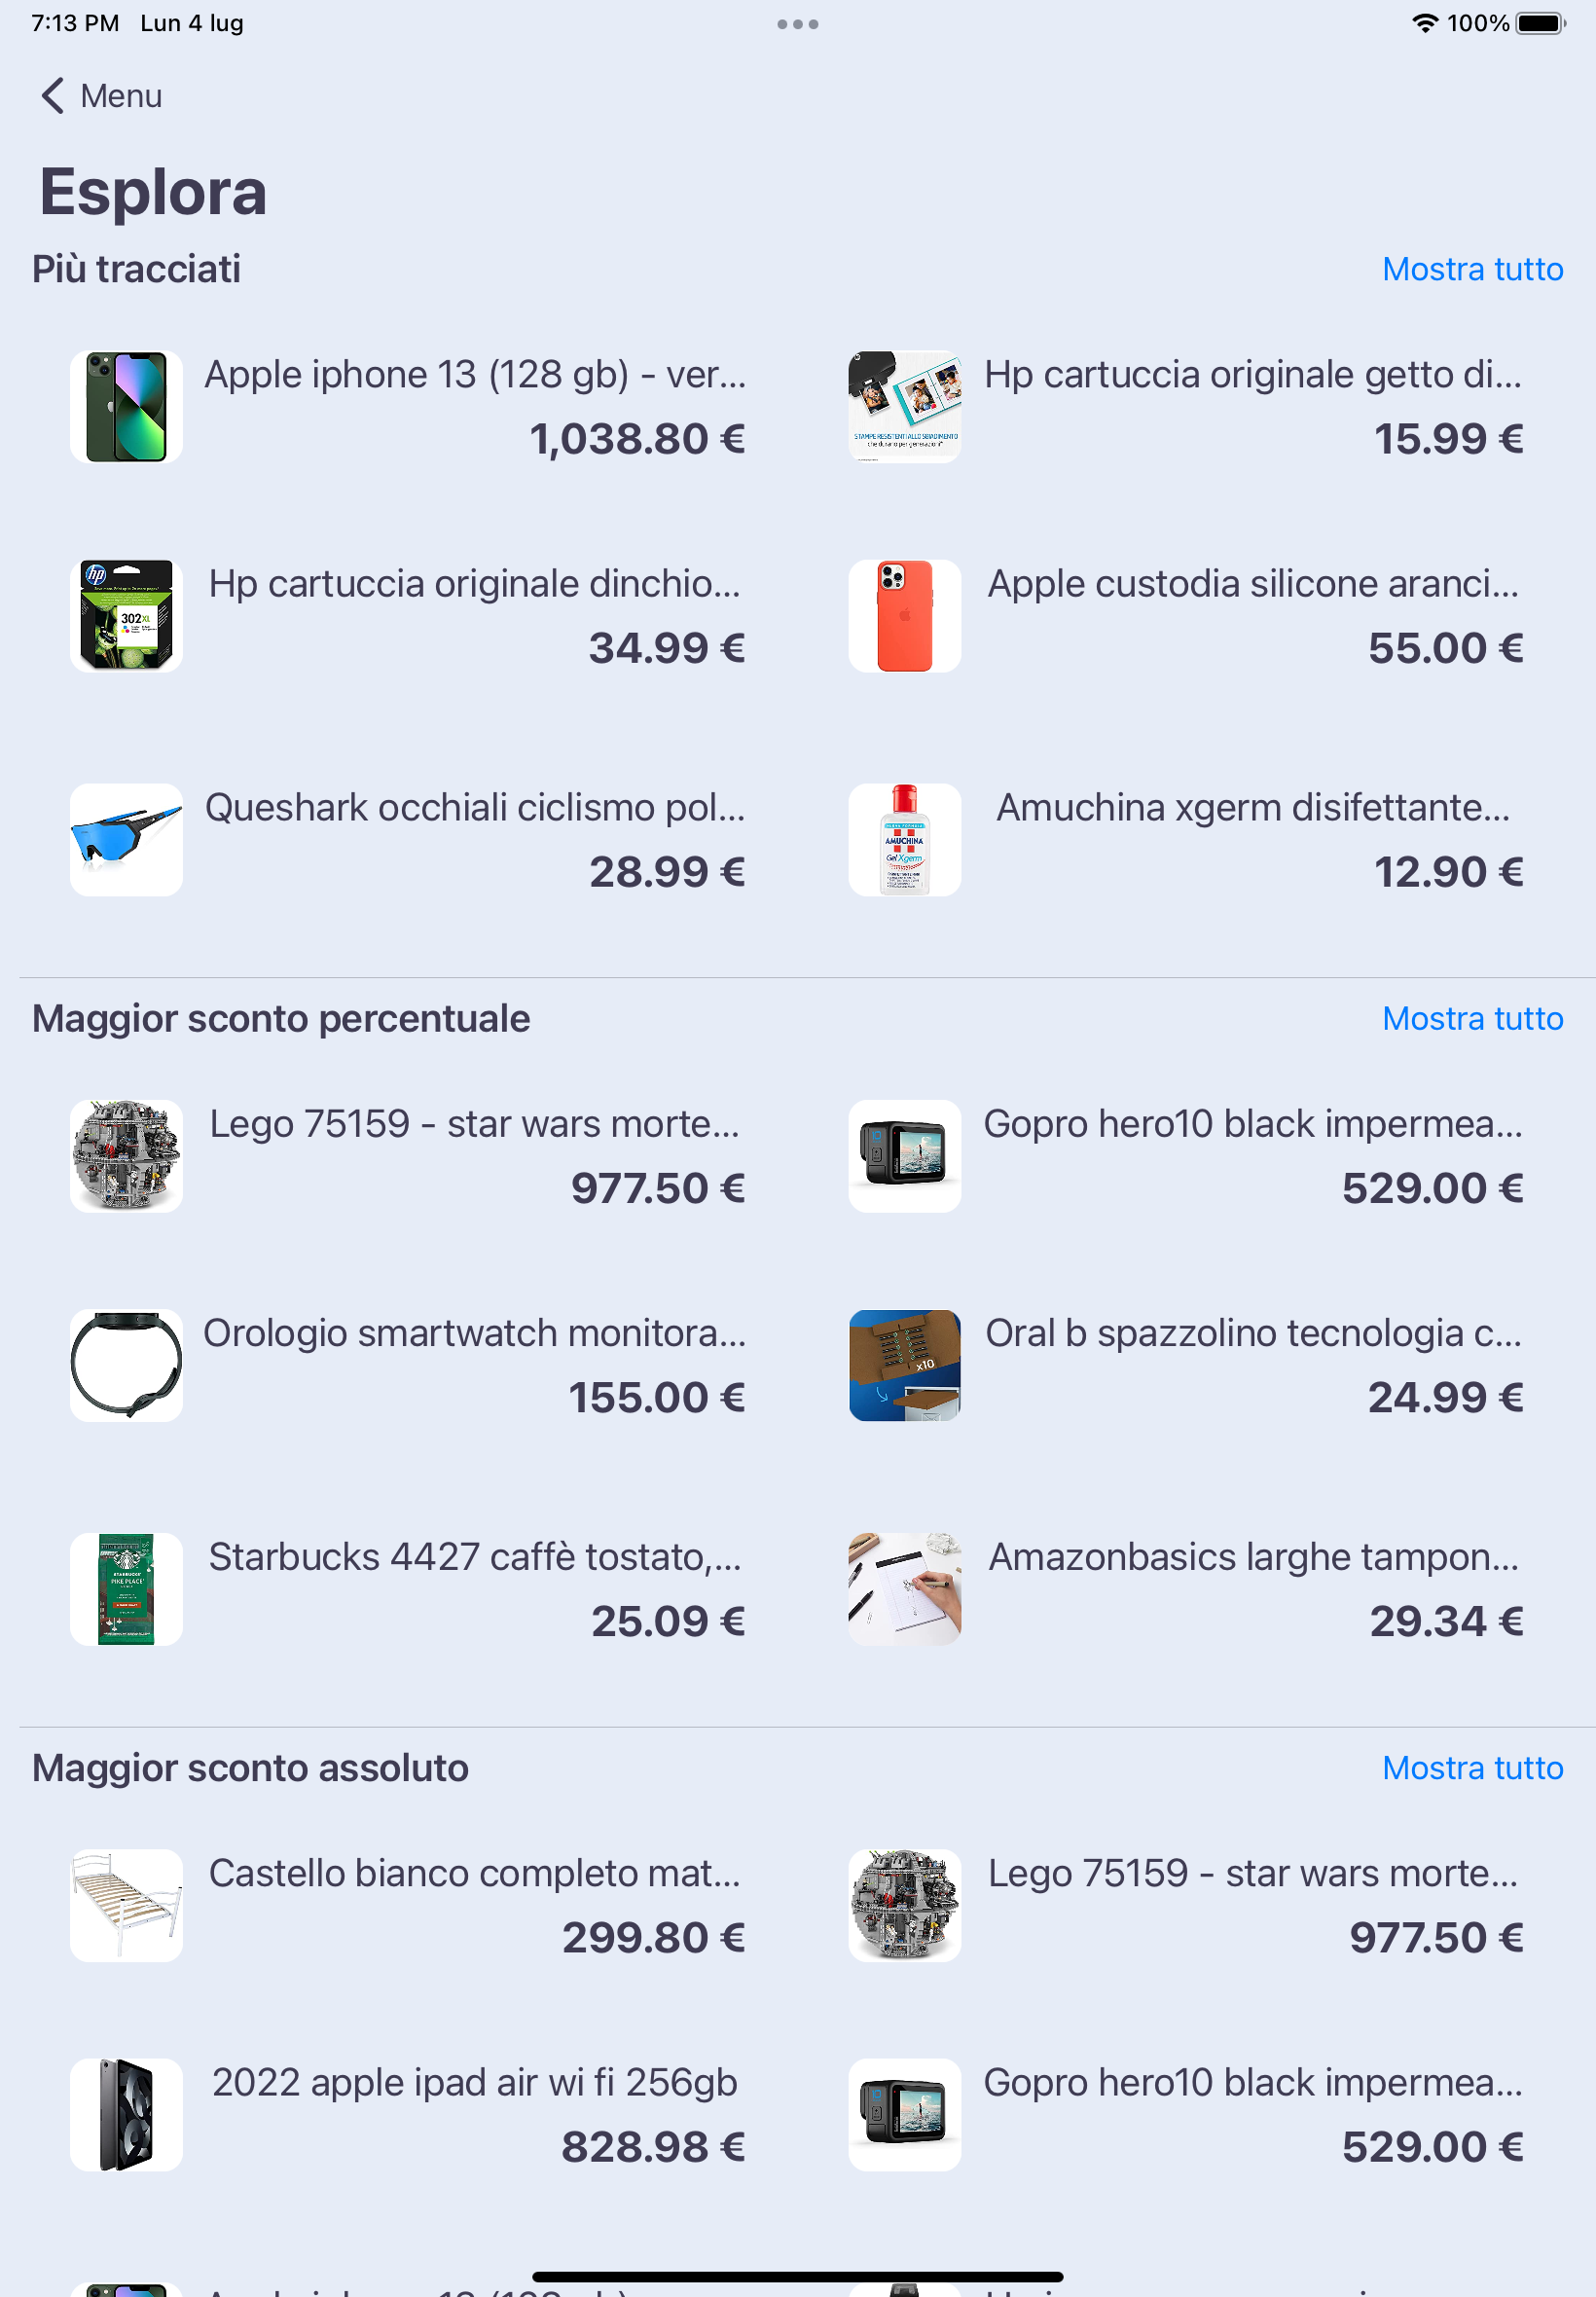
\includegraphics[width=\textwidth]{images/interfaces/explore_screen_ipad.png}
            \caption{iPad}
            \label{fig:explore_screen_ipad}
        \end{subfigure}
         \caption{Explore screen}
        \label{fig:explore_screen}
\end{figure}
\FloatBarrier
This is the explore view (fig: \ref{fig:explore_screen}). From here the user can see three different interesting sections (on how the products are ordered):
\begin{itemize}
    \item \textbf{Most tracked:} the most tracked product by application users are shown.
    \item \textbf{Biggest percentual drop:} product are ordered by percentual difference on price
    \item \textbf{Biggest range drop:} here are present the products that have had the highest range drop between maximum value and minimum value.
\end{itemize}

From all the described section (and also from the home) the complete list can be displays by clicking on the "See all" button near the section name:

\begin{figure}[h!]
        \centering
        \begin{subfigure}[b]{0.3\textwidth}
            \centering
            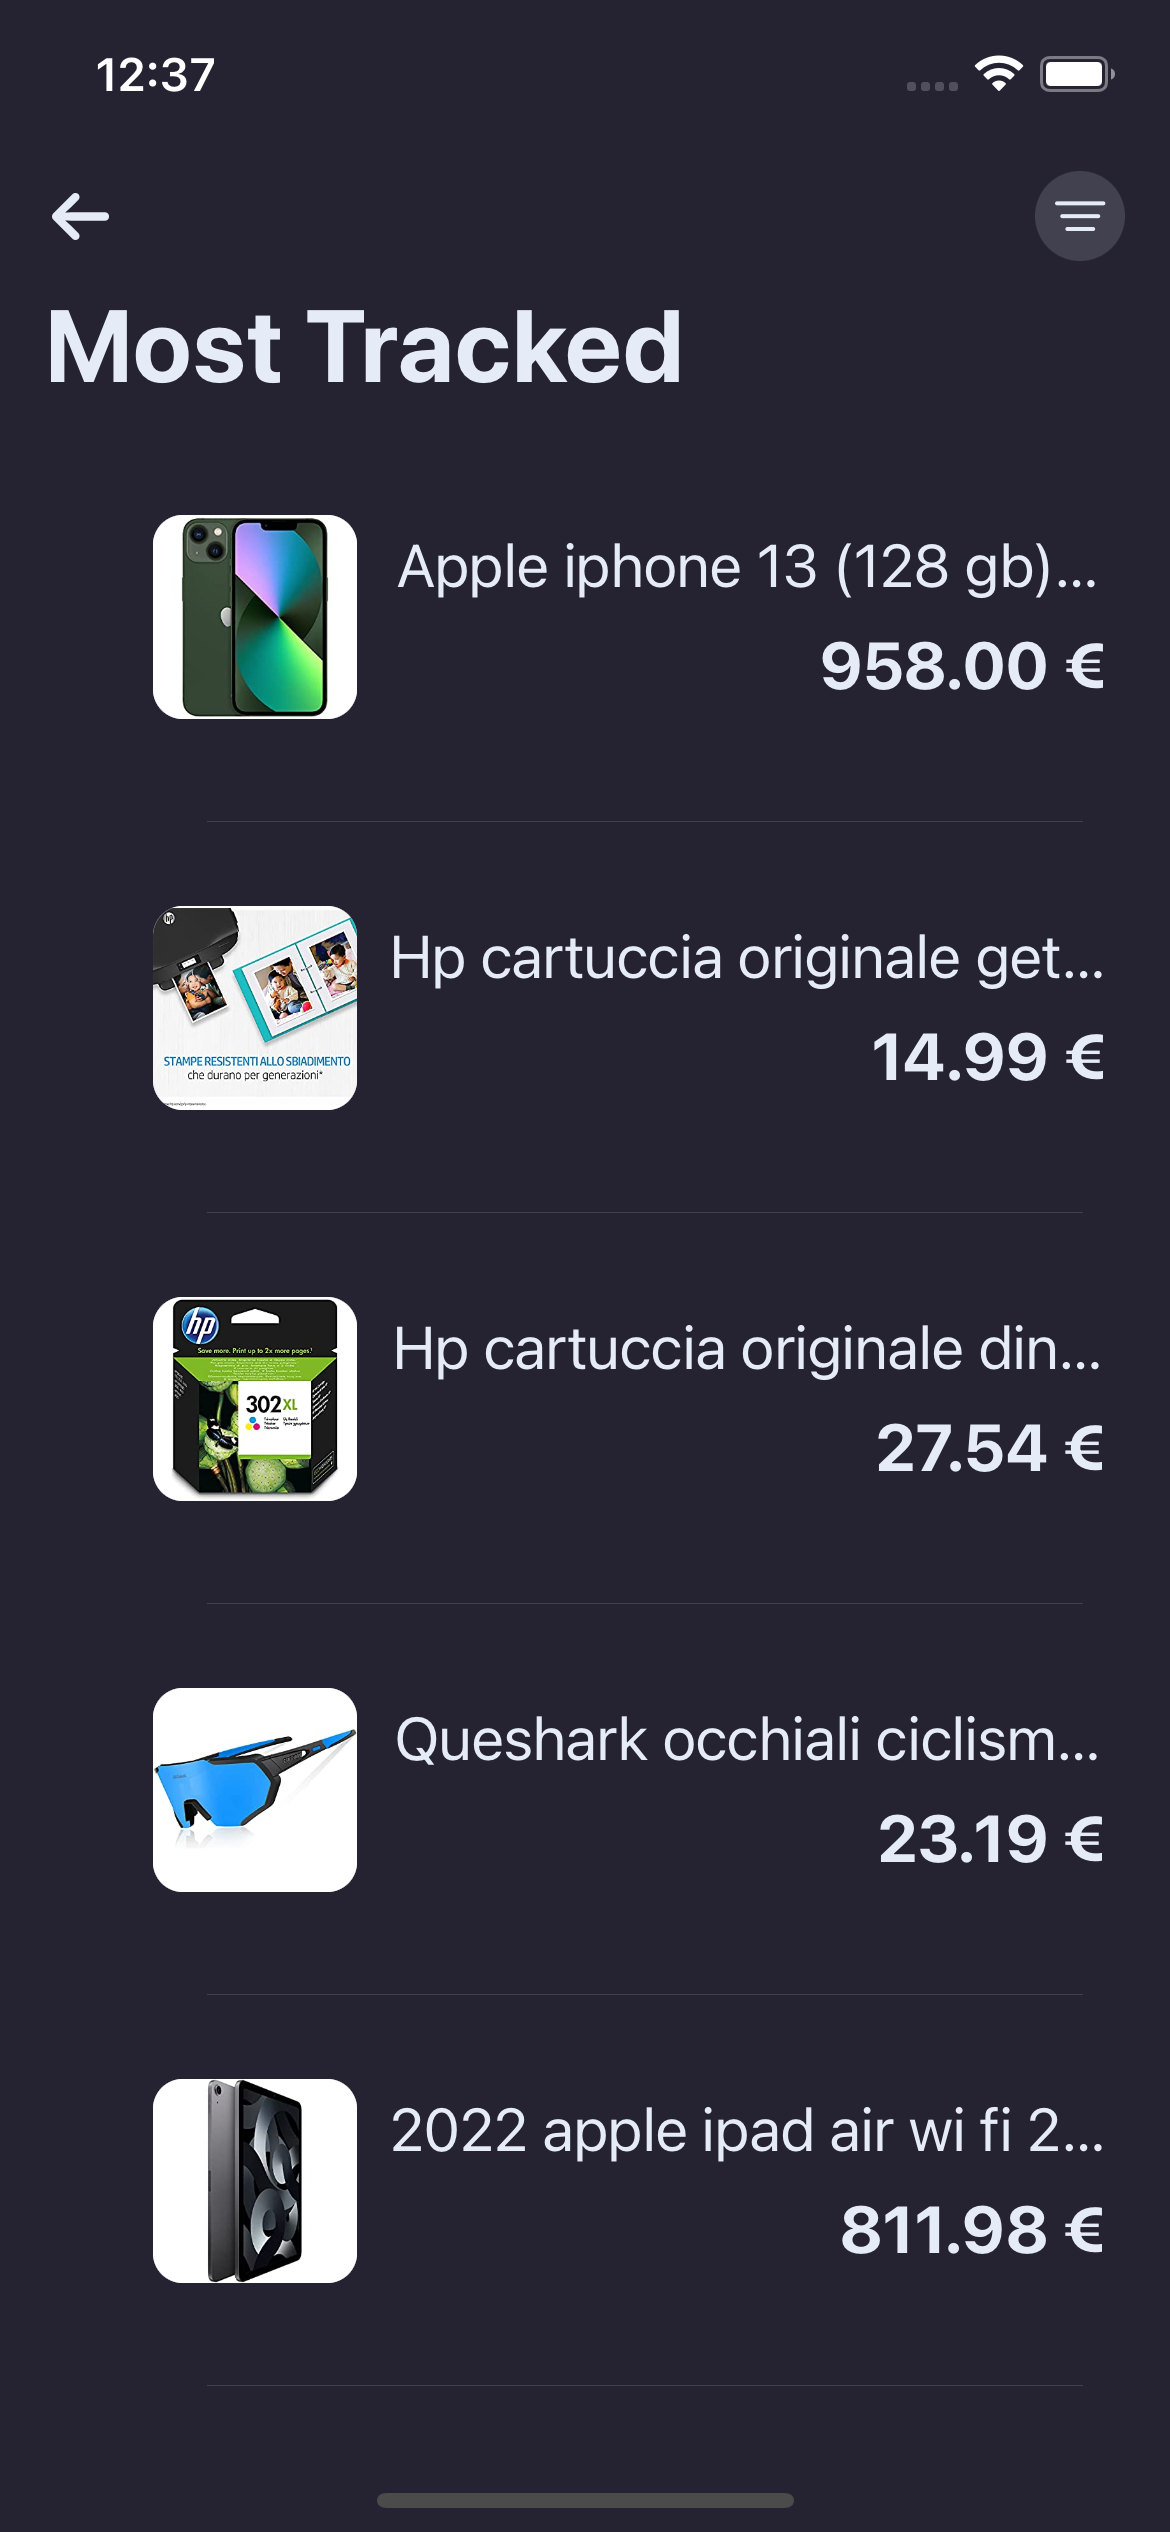
\includegraphics[width=\textwidth]{images/interfaces/see_all_explore_screen.png}
            \caption{iPhone}
            \label{fig:see_all_explore_screen_iphone}
        \end{subfigure}
        \begin{subfigure}[b]{0.45\textwidth}
            \centering
            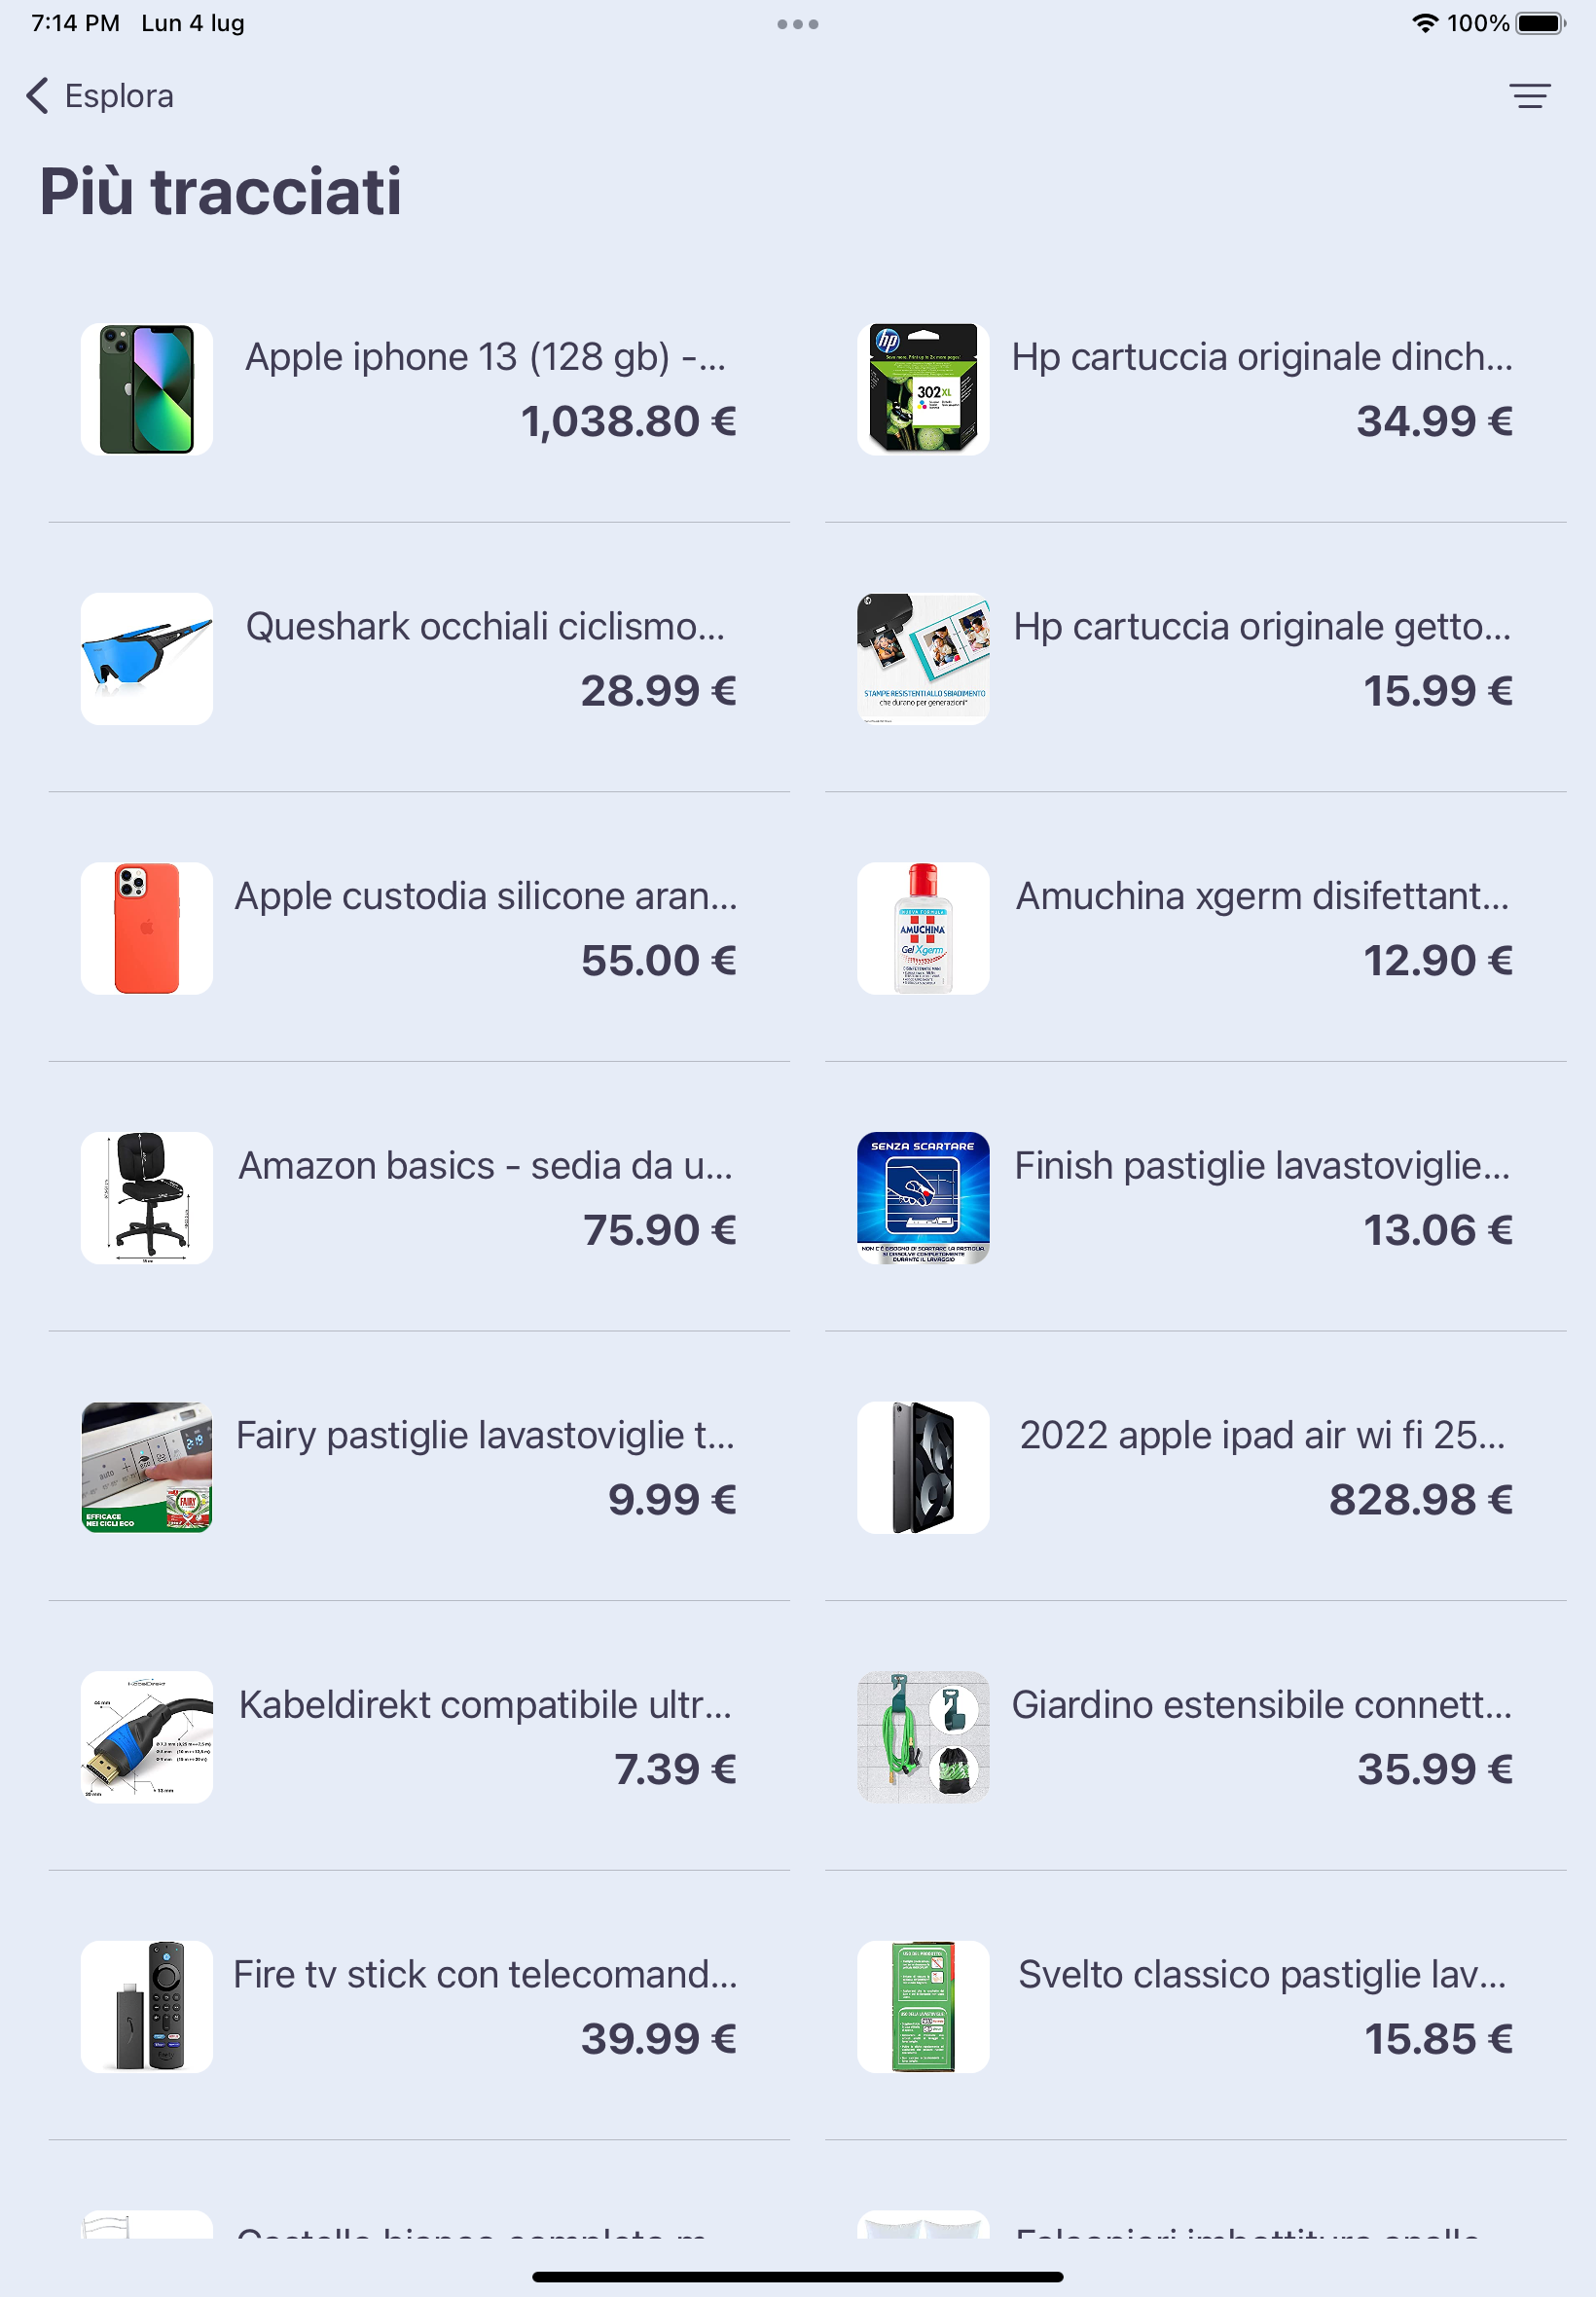
\includegraphics[width=\textwidth]{images/interfaces/see_all_explore_screen_ipad.png}
            \caption{iPad}
            \label{fig:see_all_explore_screen_ipad}
        \end{subfigure}
         \caption{See all explore screen}
        \label{fig:see_all_explore_screen}
\end{figure}
\FloatBarrier
This is the see all view, all the products of the selected section are present (fig: \ref{fig:see_all_explore_screen}).\\
This view is an infinite scrollable vertical stack view, where at first will be load only a certain amount of product and while scrolling down more product will be added to the stack dynamically.
In this view it is also present a button in the top-right corner to filter them based on the category.

\begin{figure}[h!]
        \centering
        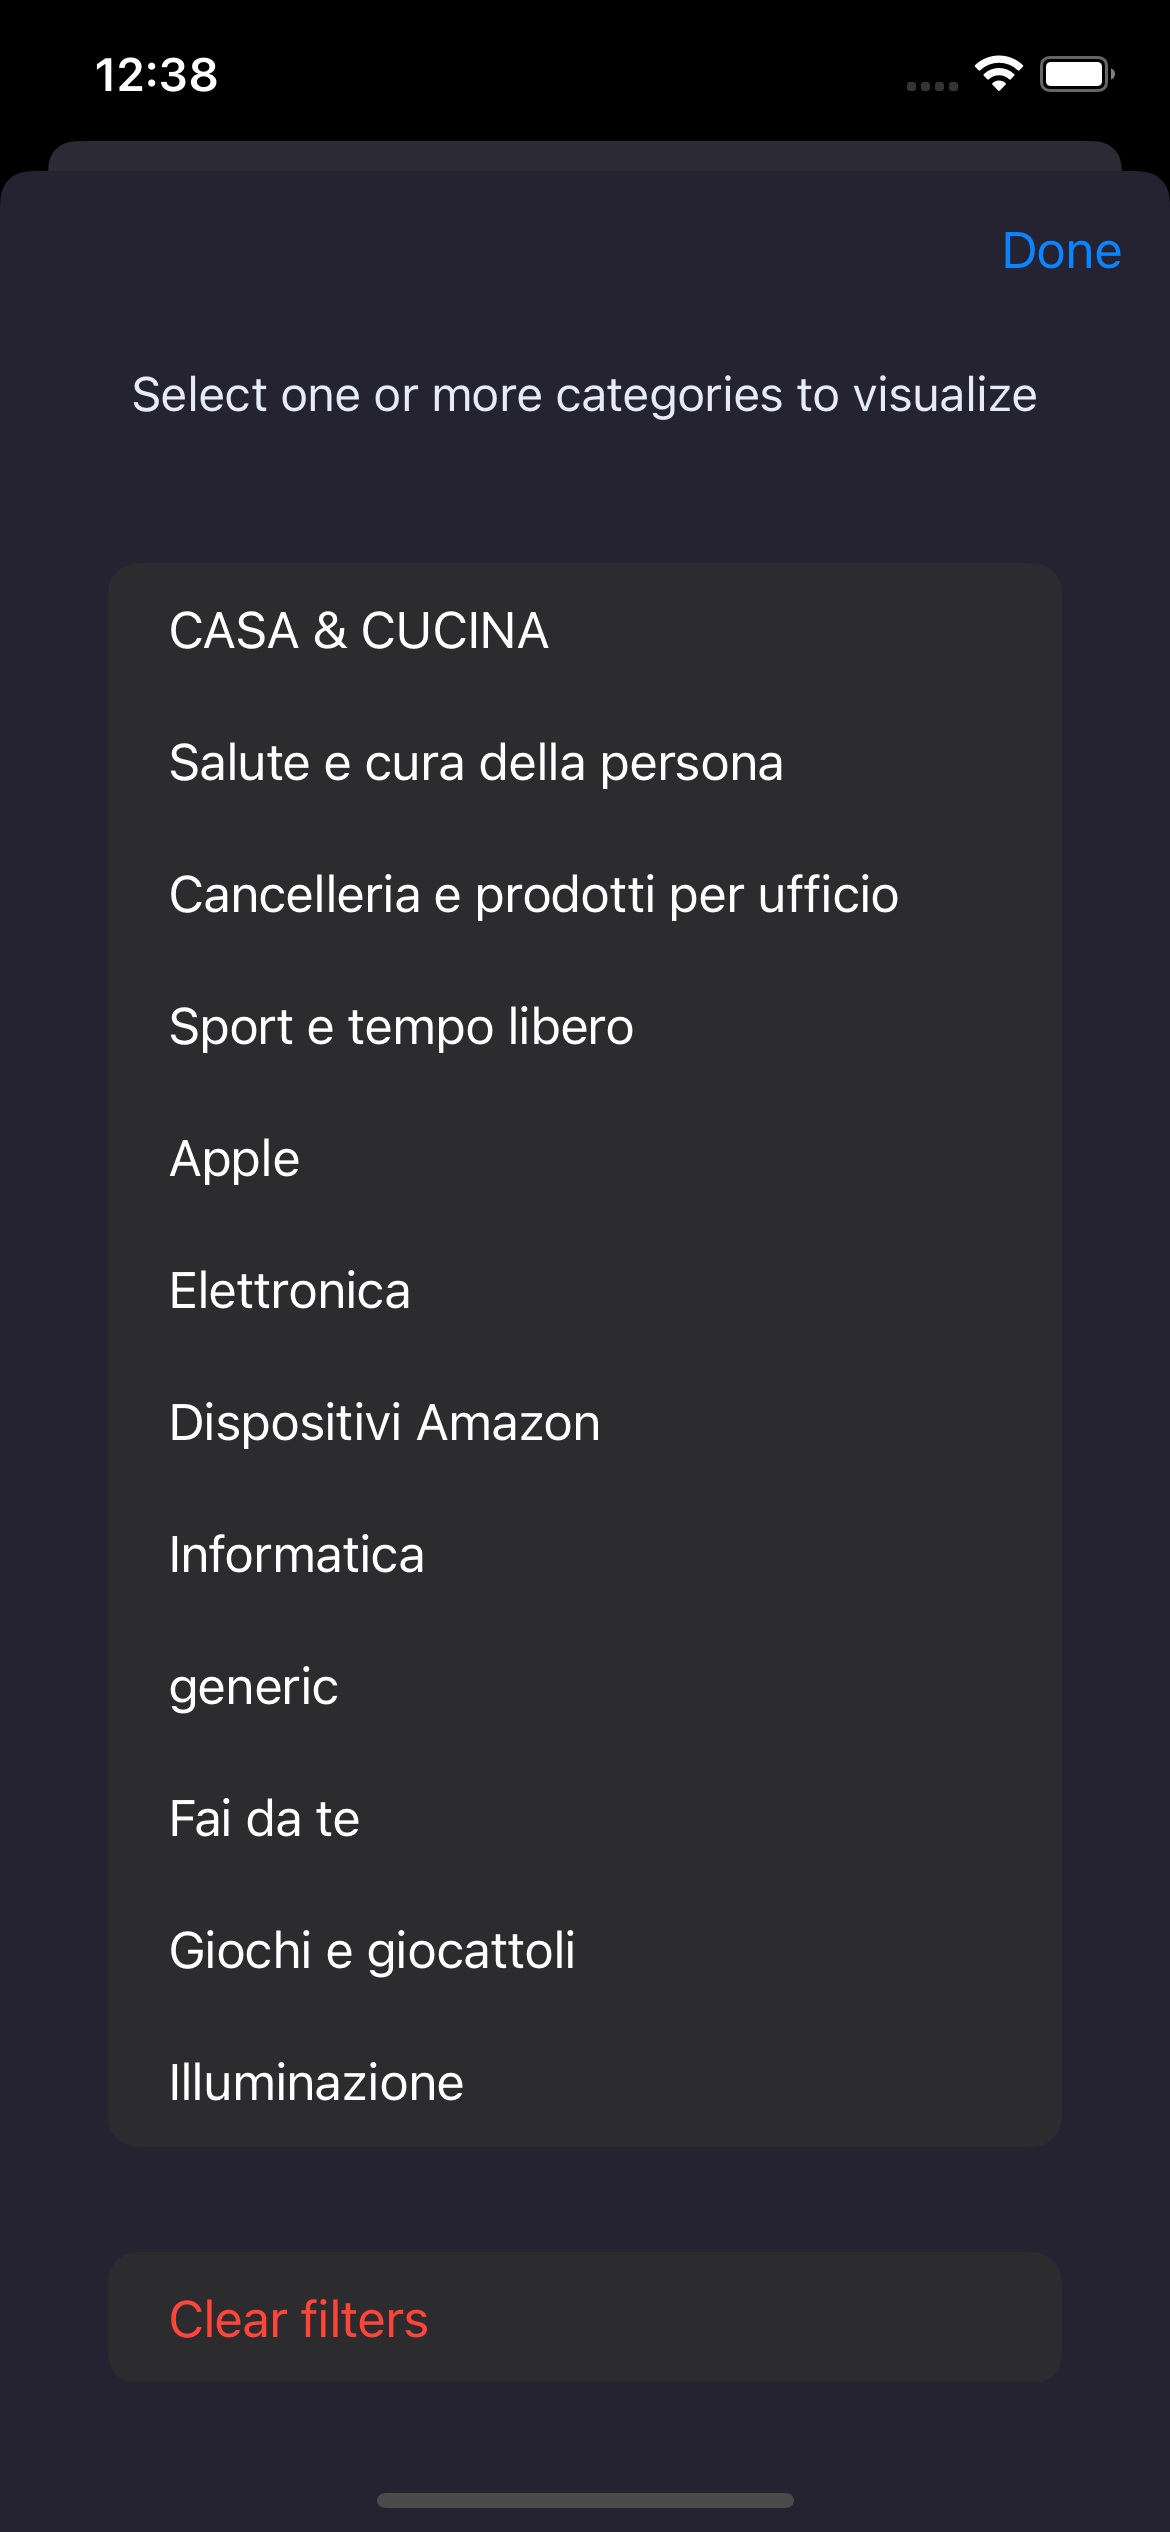
\includegraphics[scale=0.15]{images/interfaces/category_selection_screen.png}
        \caption{Category selection screen}
        \label{fig:category_selection_screen}
\end{figure}
\FloatBarrier
This view (fig: \ref{fig:category_selection_screen}) let the user filters between different categories to show only the relevant products to him. This view can be accessed from every see all section of the explore view (fig: \ref{fig:see_all_explore_screen}).

\begin{figure}[h!]
        \centering
        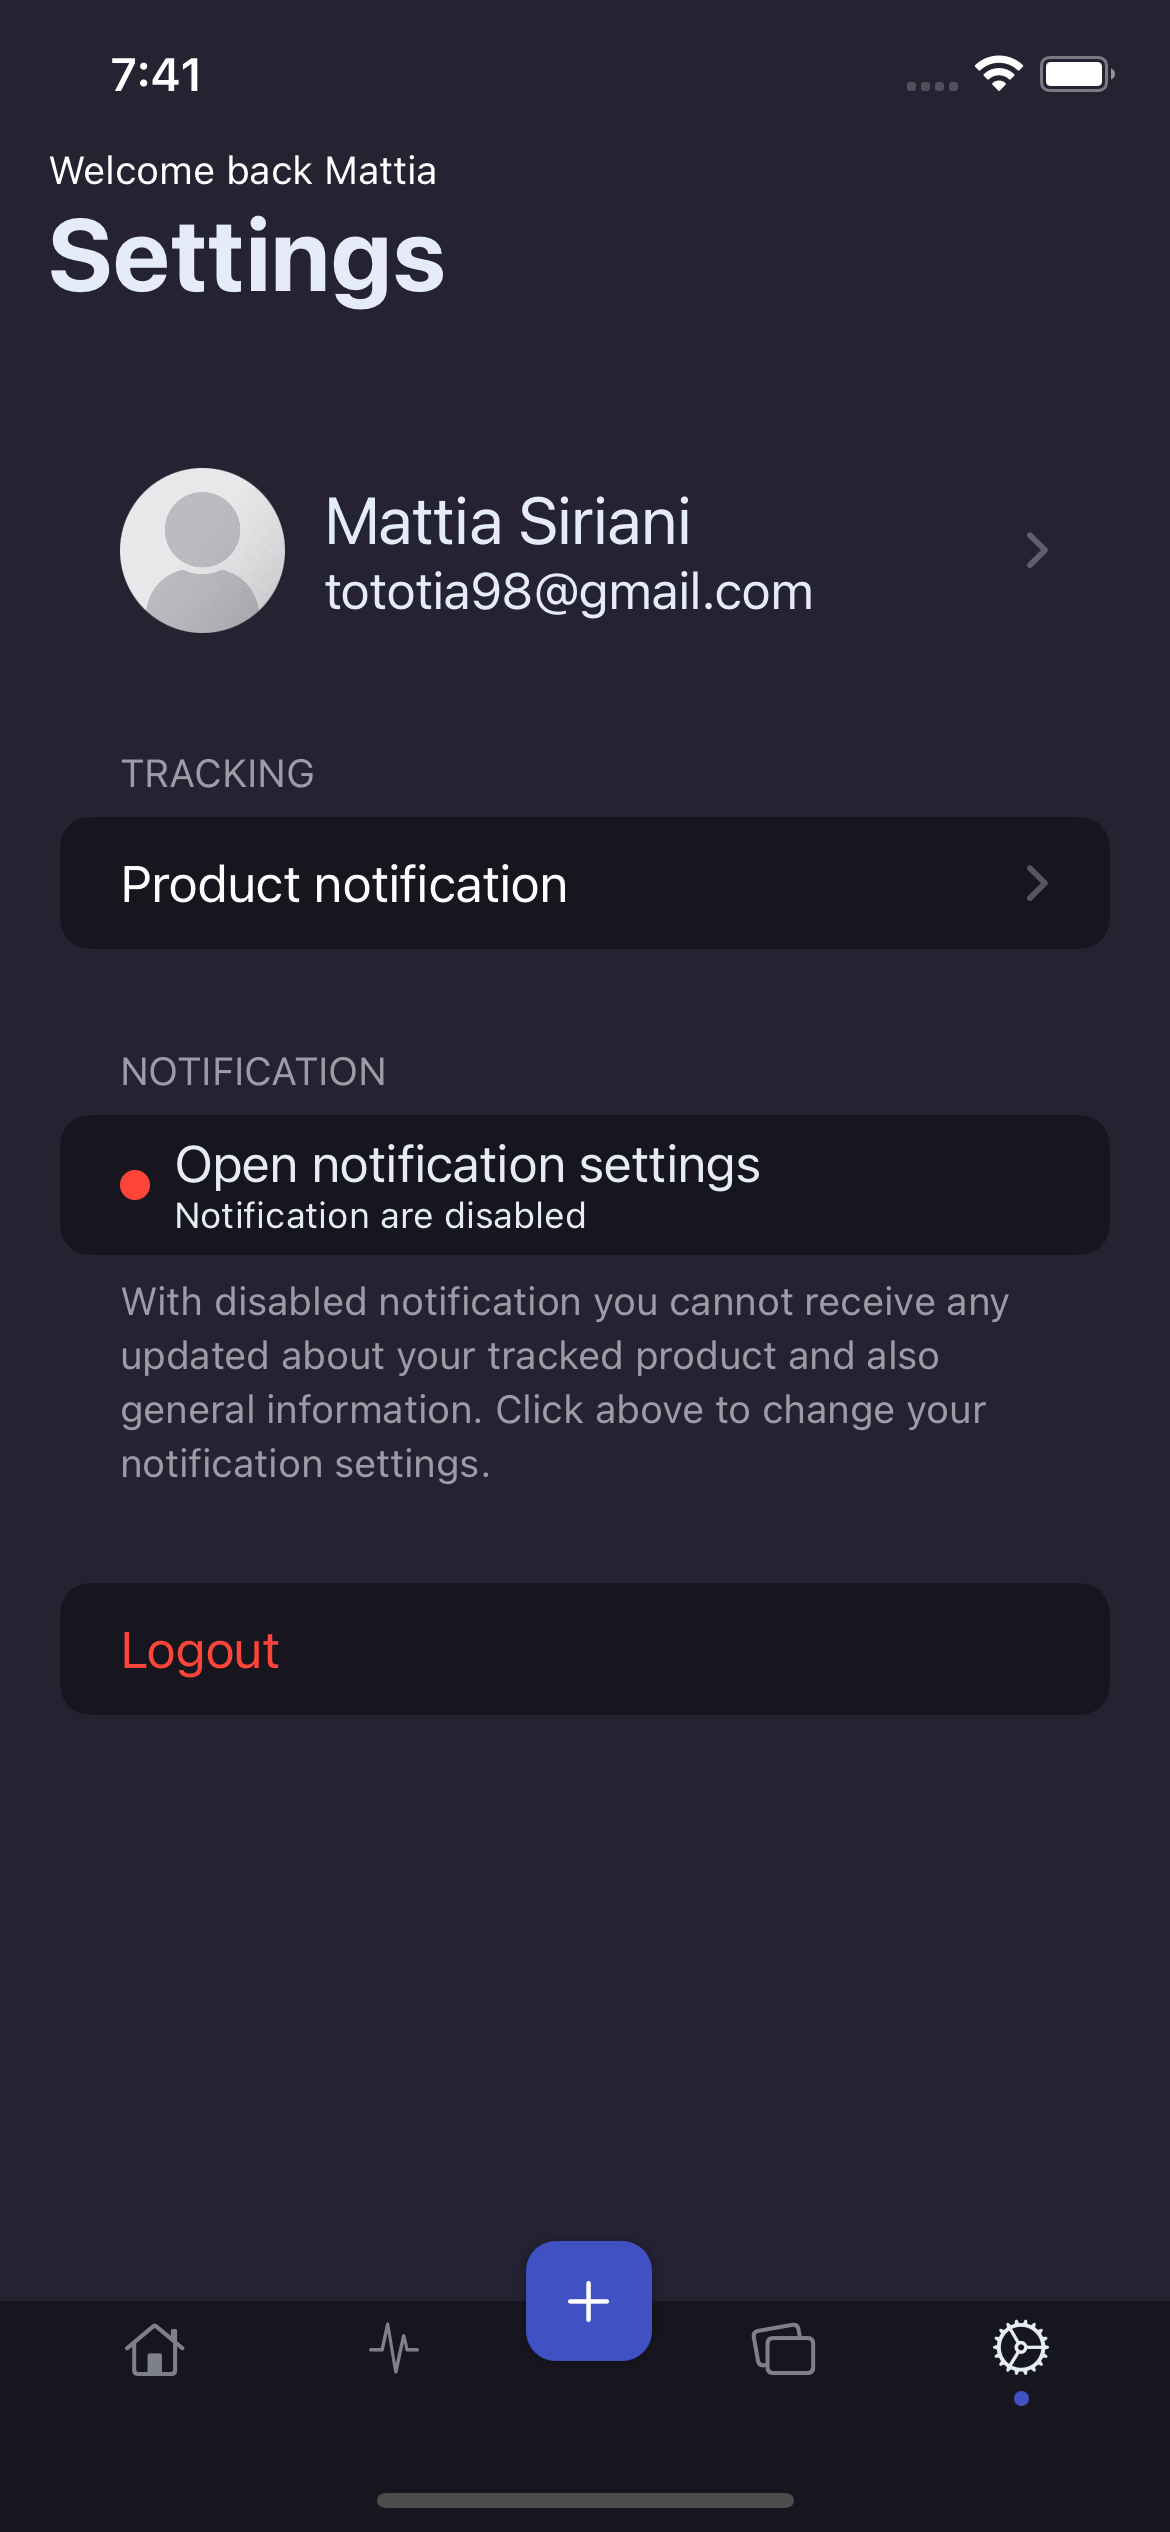
\includegraphics[scale=0.15]{images/interfaces/settings_screen.png}
        \caption{Settings screen}
        \label{fig:settings_screen}
\end{figure}
\FloatBarrier
This is the settings view when the user is logged (fig: \ref{fig:settings_screen}). From here the user can access to his personal information and modify them, change the general product notification (default value that triggers the notification, assigned to a product when is being tracked by the user), open the notification settings of the device and Logout.

\begin{figure}[h!]
        \centering
        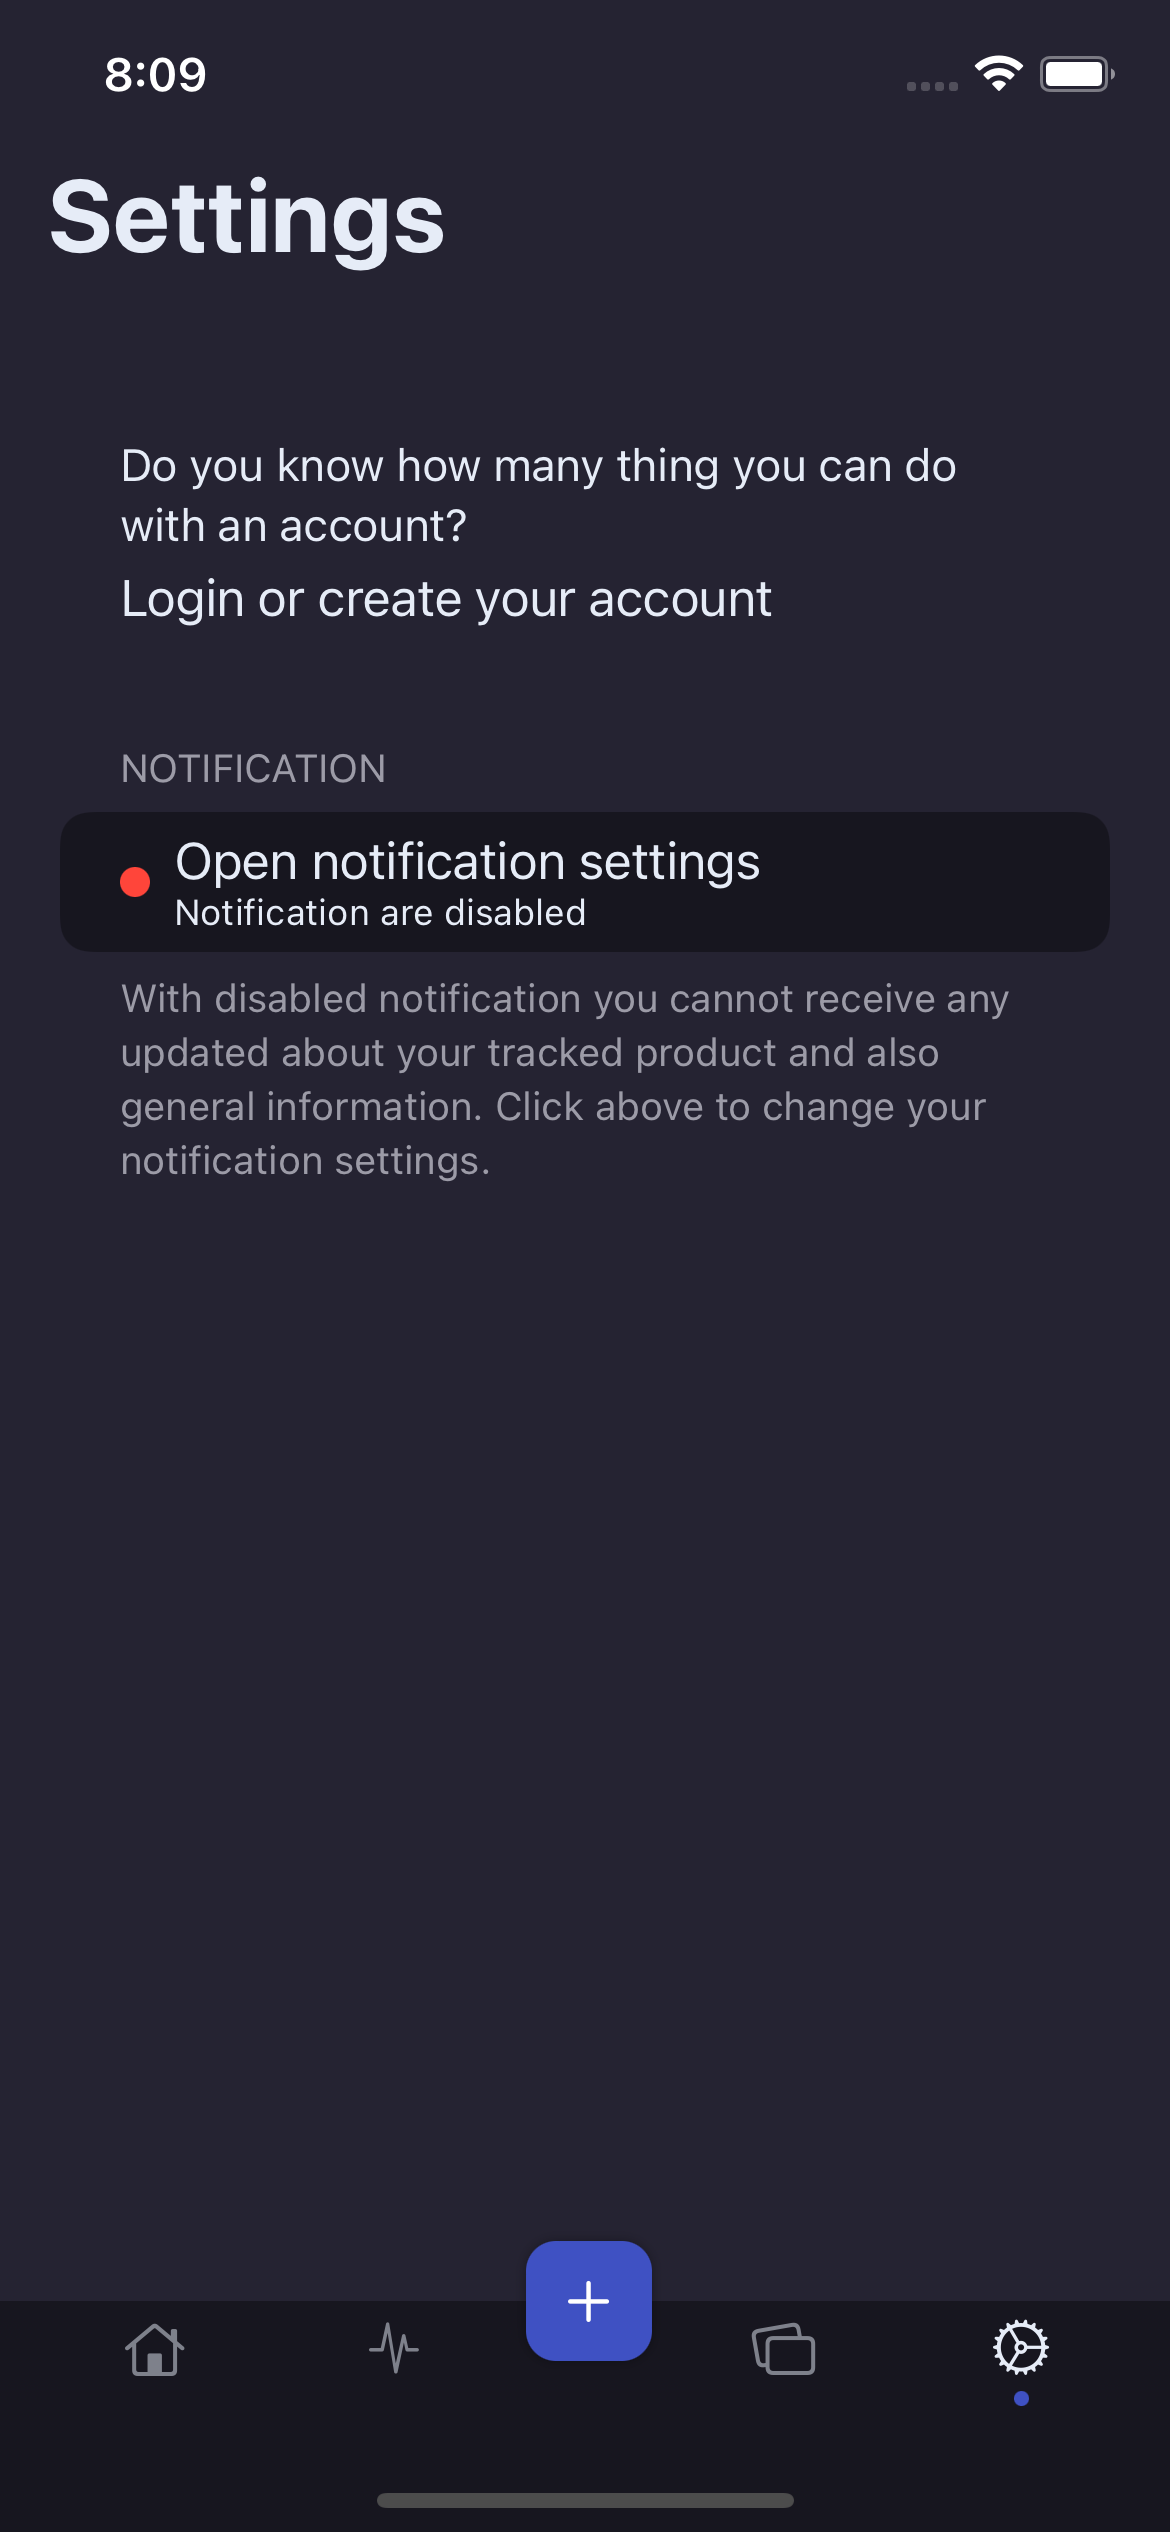
\includegraphics[scale=0.15]{images/interfaces/settings_screen_not_logged.png}
        \caption{Settings screen, if user is not logged}
        \label{fig:settings_screen_not_logged}
\end{figure}
\FloatBarrier
This is the settings view when the user is not logged (fig: \ref{fig:settings_screen_not_logged}). From here the user can login in the application and open the notification settings of the device.

\begin{figure}[h!]
        \centering
        \begin{subfigure}[b]{0.3\textwidth}
            \centering
            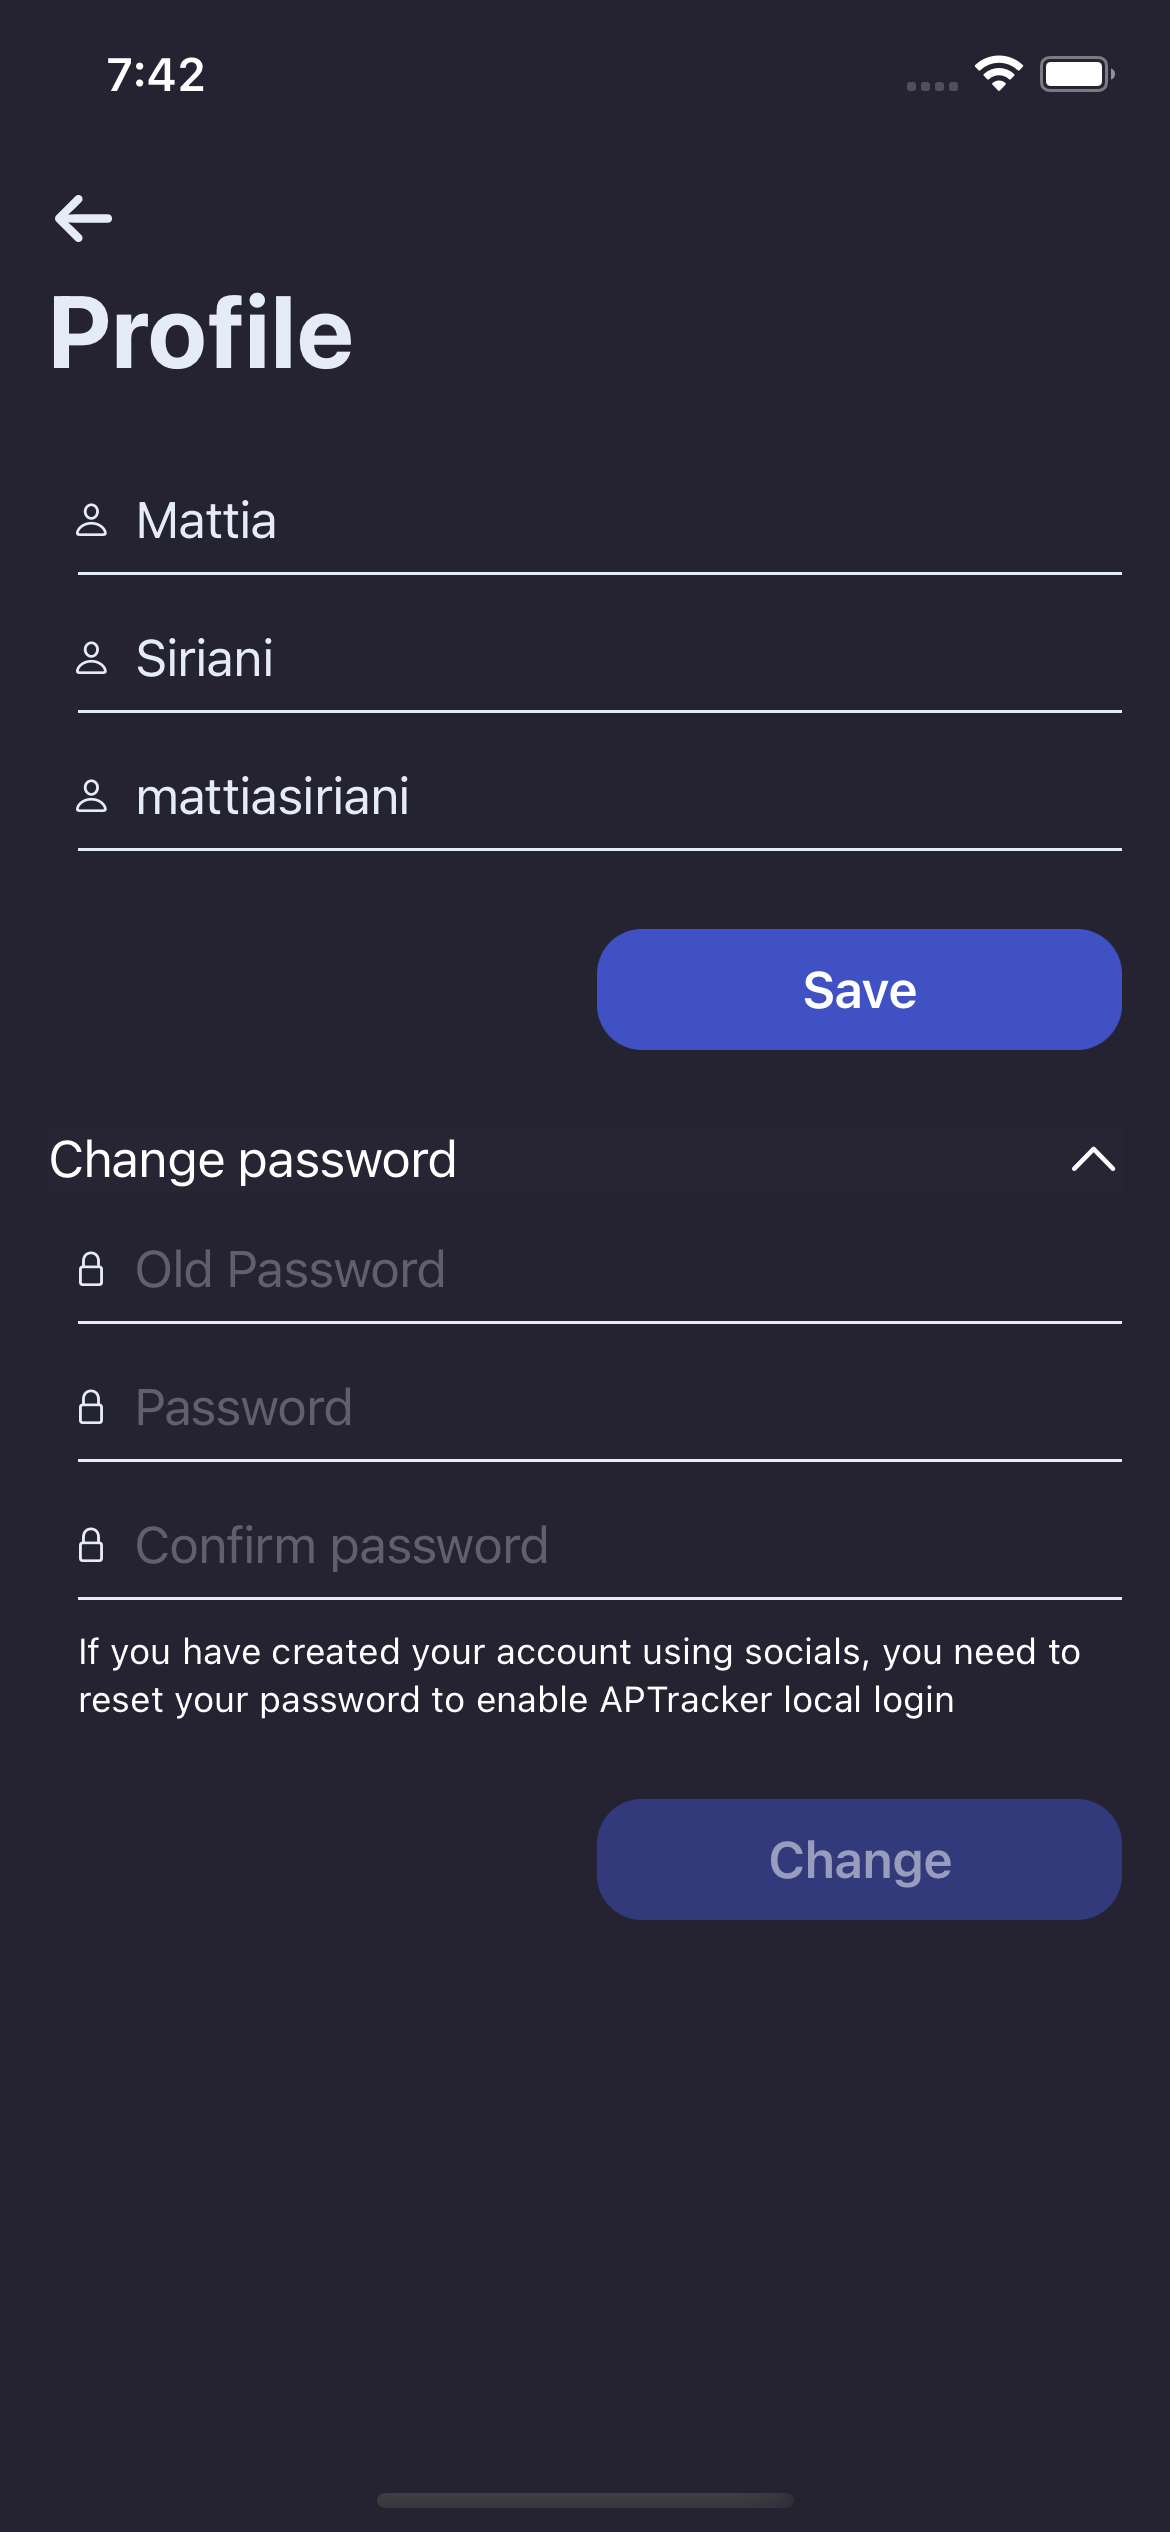
\includegraphics[width=\textwidth]{images/interfaces/user_profile_settings_screen.png}
            \caption{iPhone}
            \label{fig:user_profile_settings_screen_iphone}
        \end{subfigure}
        \begin{subfigure}[b]{0.45\textwidth}
            \centering
            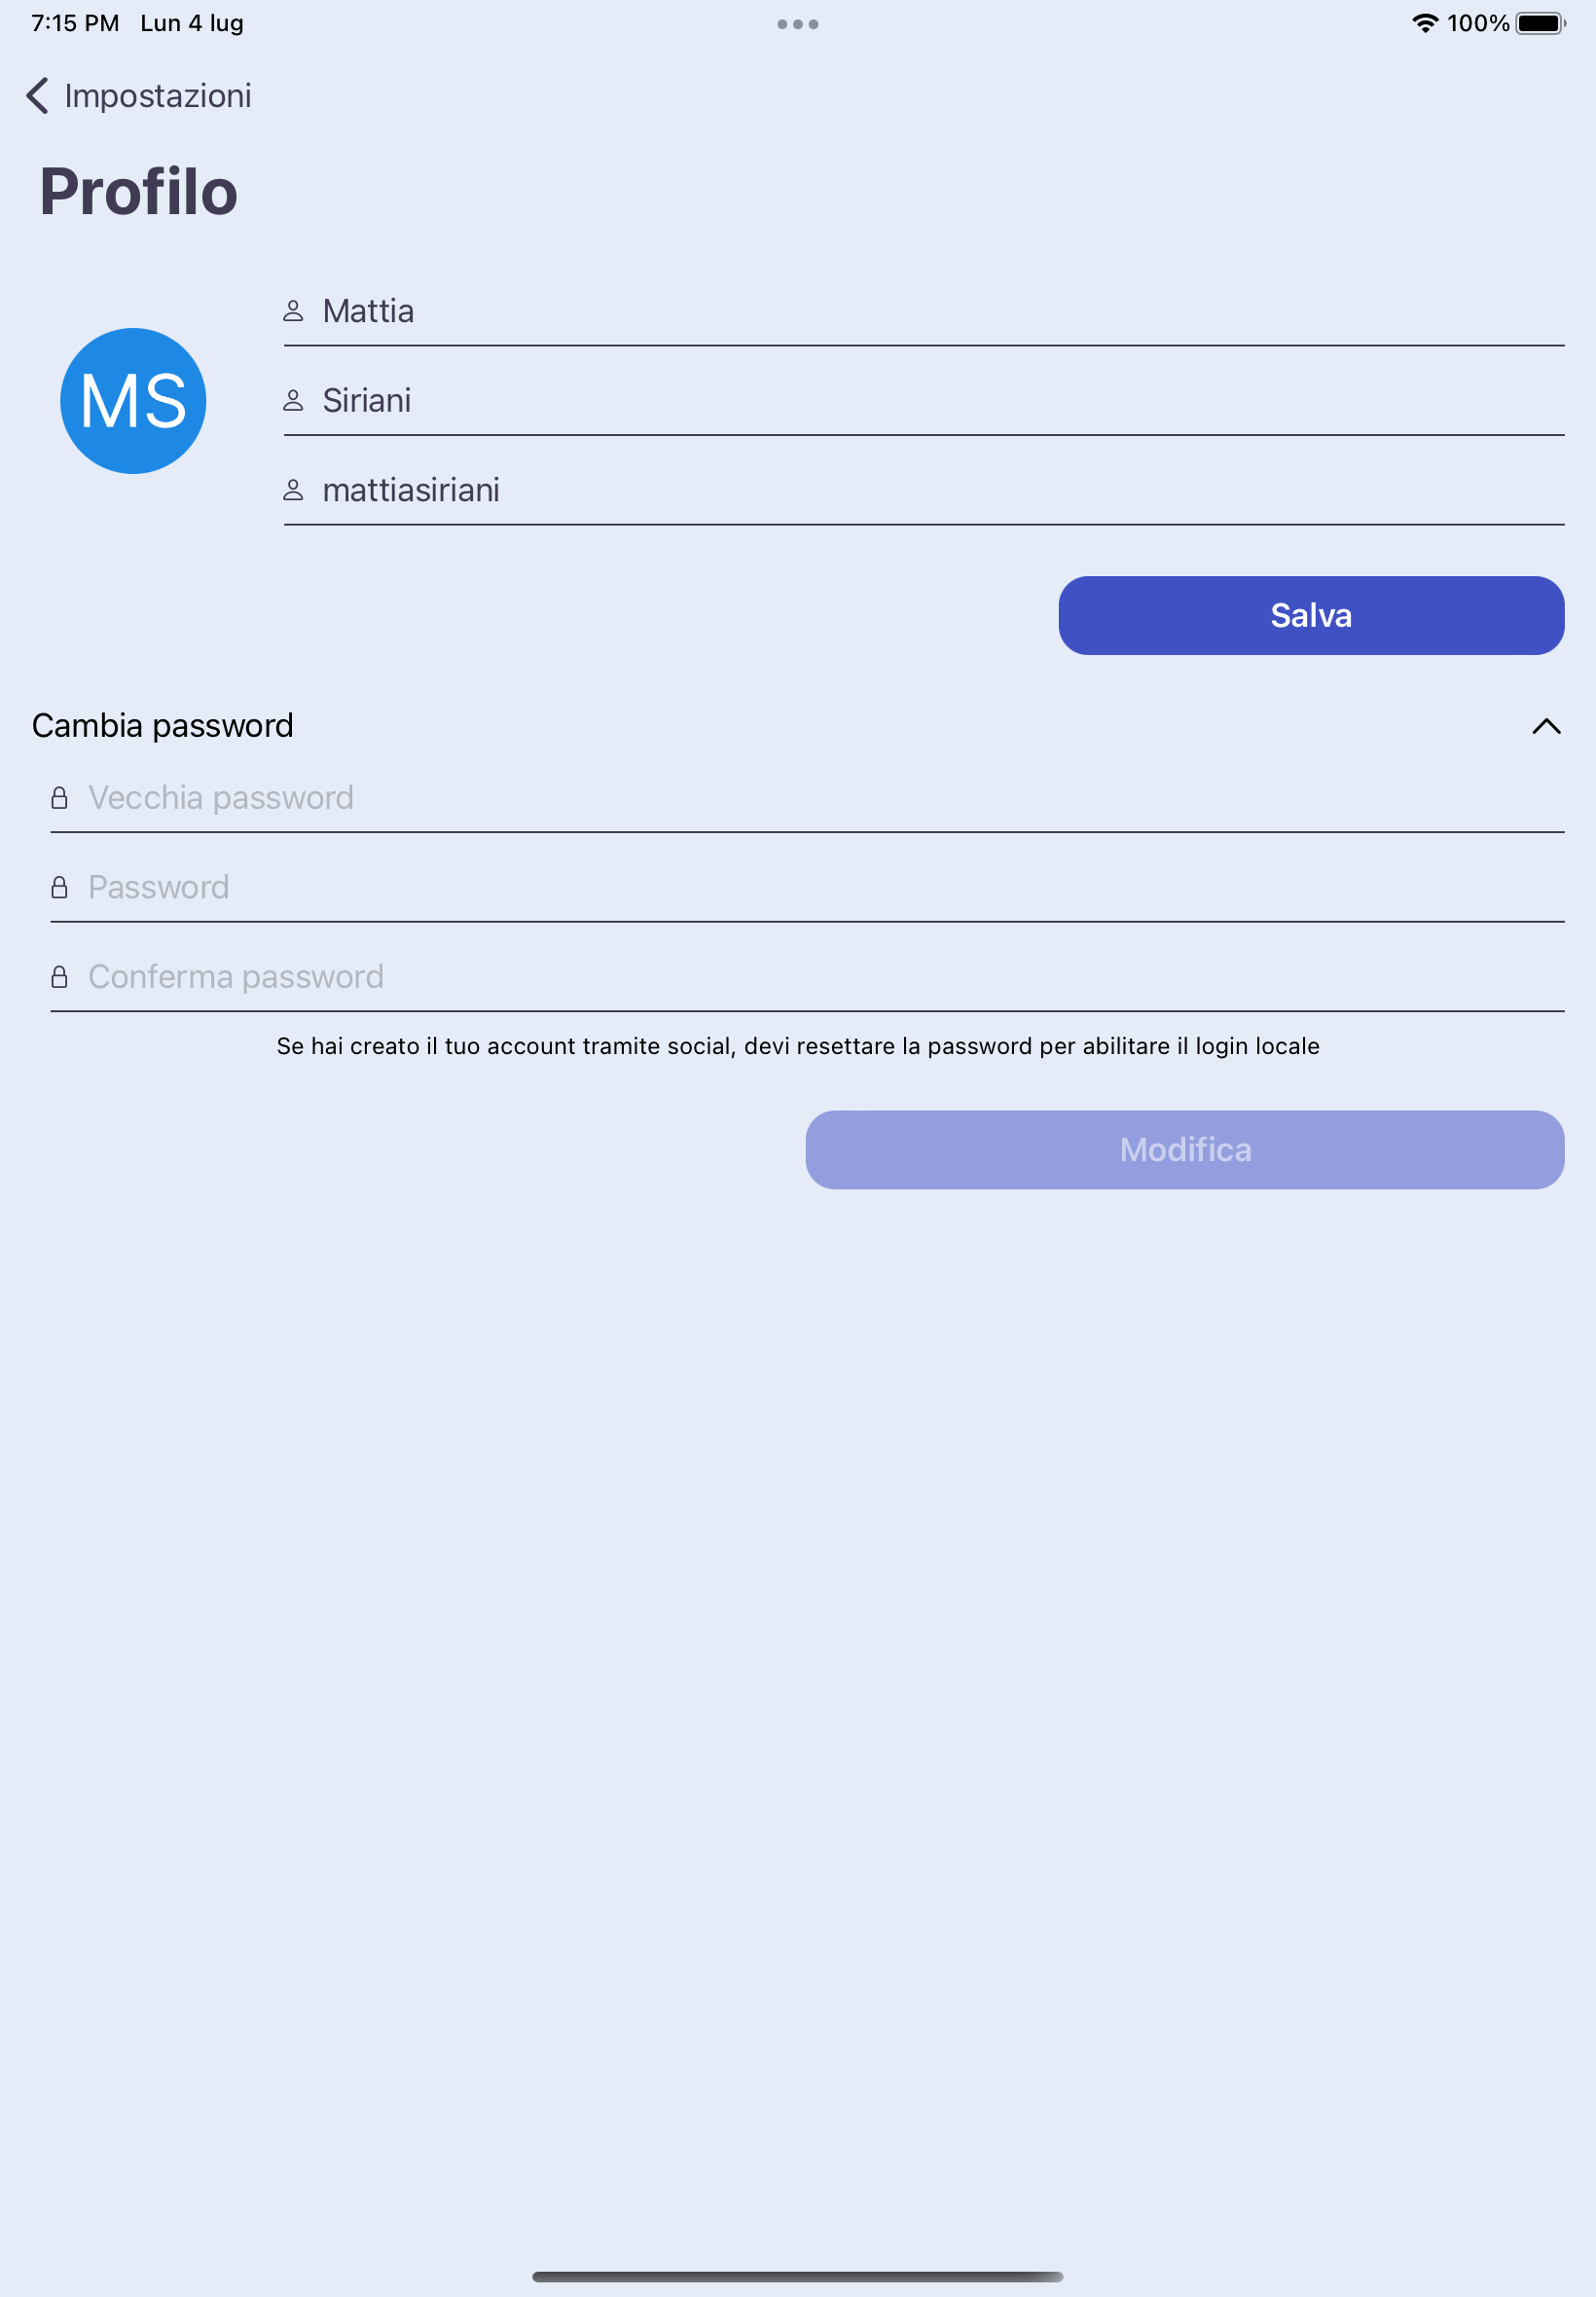
\includegraphics[width=\textwidth]{images/interfaces/user_profile_settings_screen_ipad.png}
            \caption{iPad}
            \label{fig:user_profile_settings_screen_ipad}
        \end{subfigure}
         \caption{User profile settings screen}
        \label{fig:user_profile_settings_screen}
\end{figure}
\FloatBarrier
This is the view where the user can access his personal information(fig: \ref{fig:user_profile_settings_screen}). From here the user can change his personal information, such as name, surname, nickname, and password.\\\\

For the views regarding a product, there are always present three tab buttons that brings to:
\begin{itemize}
    \item \textbf{Price view:} containing price information.
    \item \textbf{Detail view:} containing details of the product.
    \item \textbf{Comments view:} containing comments on the product leaved by other application users.
\end{itemize}
It is also present an horizontal stack at the bottom of the screen containing the actual price of the product and a link to open the product in the Amazon website.
\begin{figure}[h!]
        \centering
        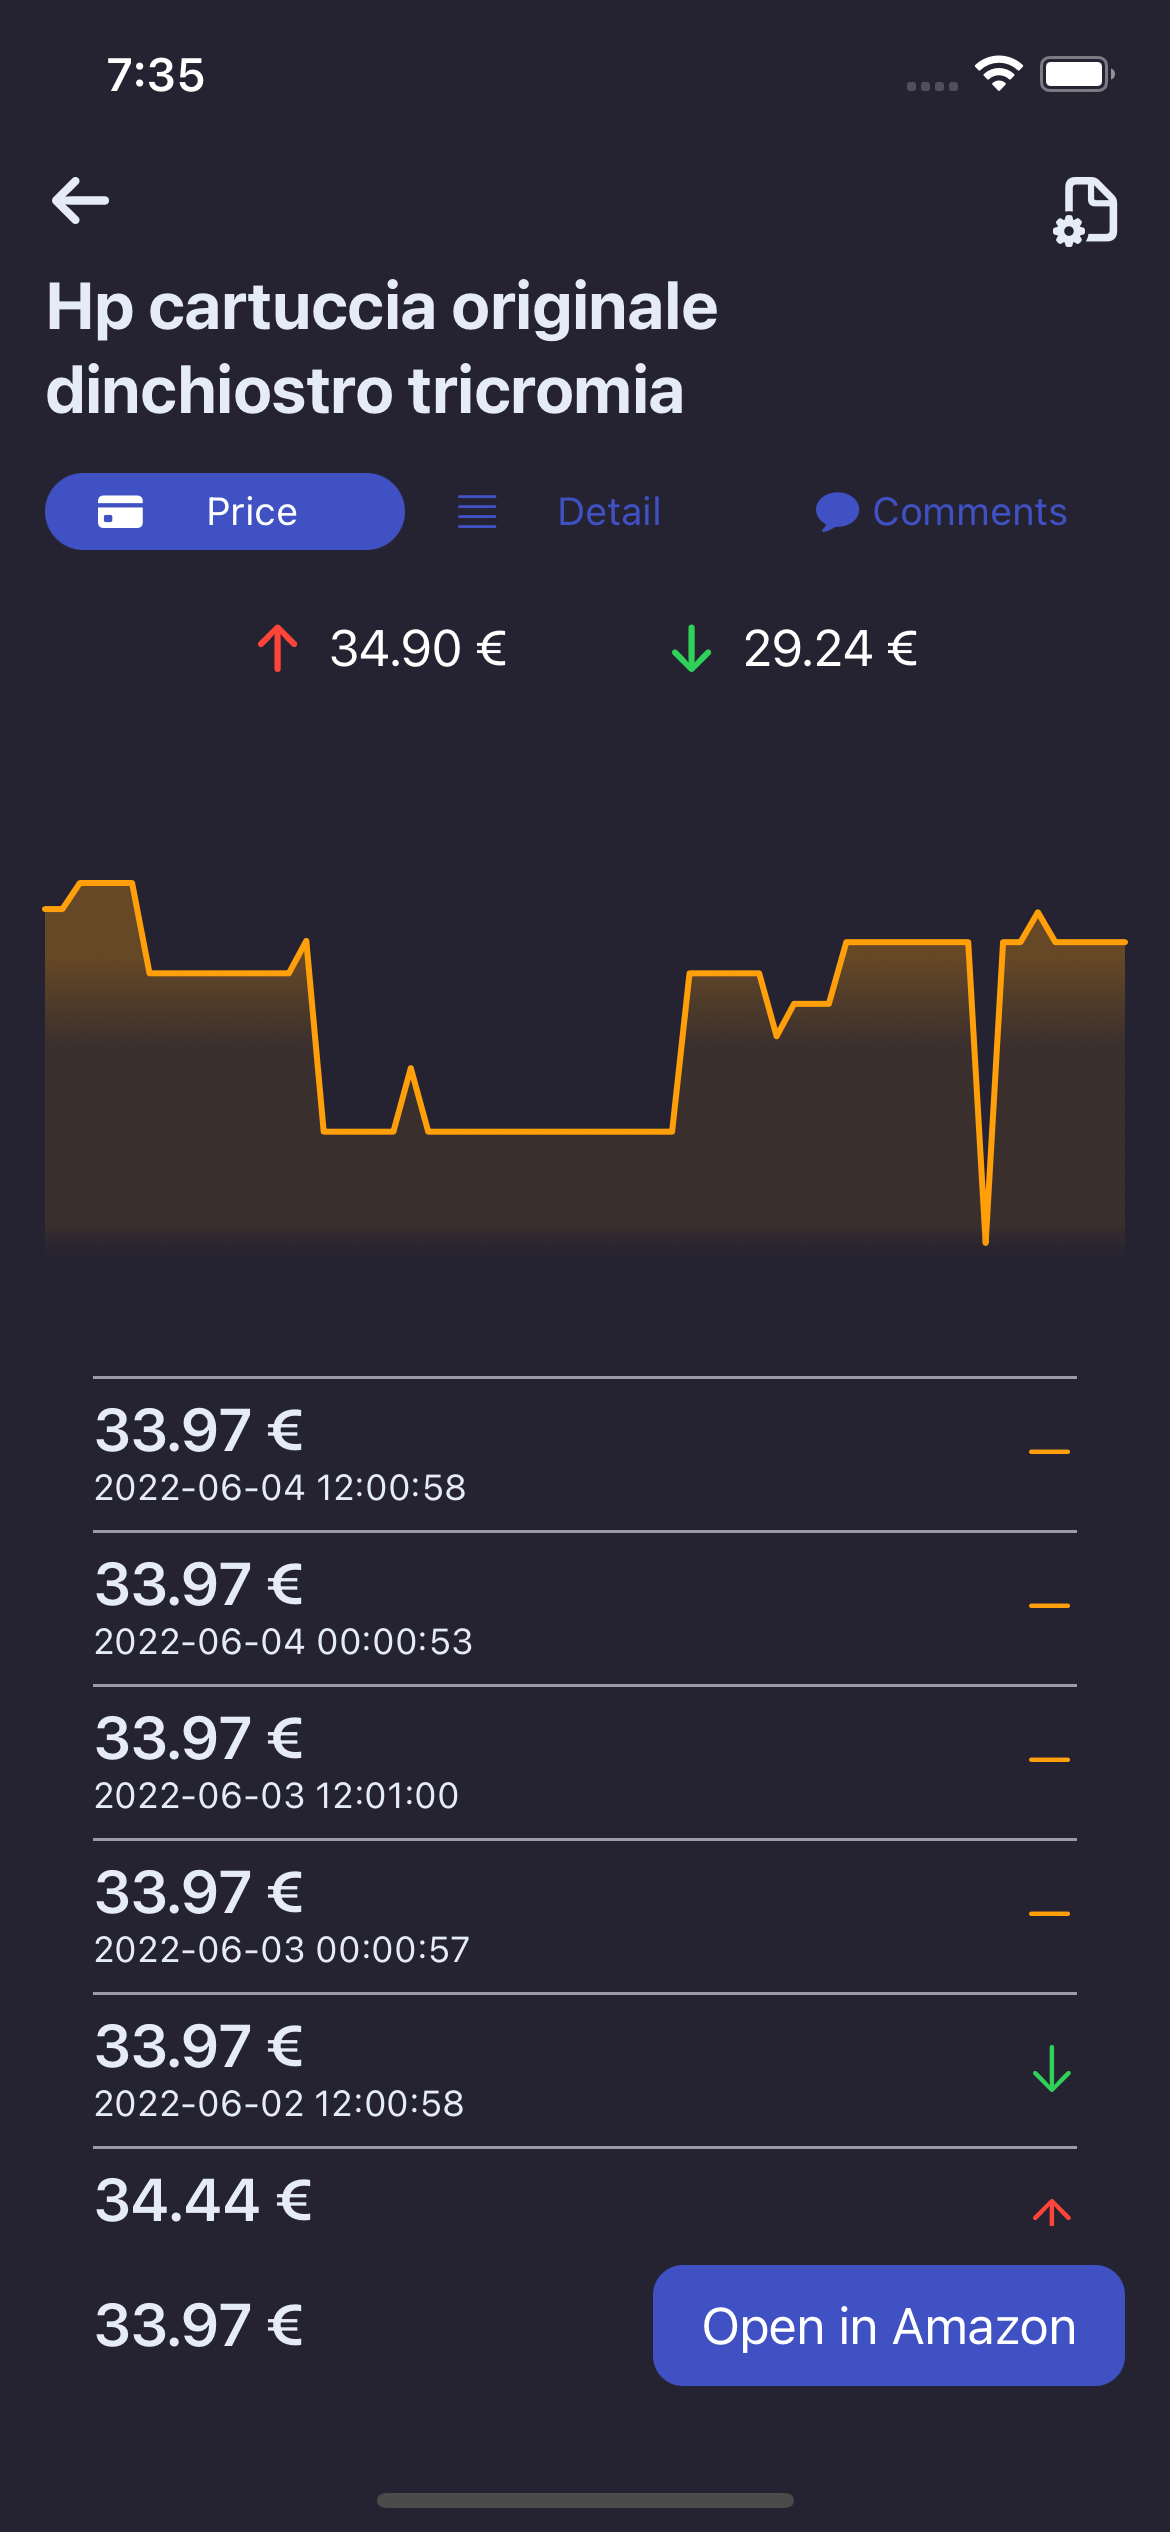
\includegraphics[scale=0.15]{images/interfaces/product_screen.png}
        \caption{Product screen}
        \label{fig:product_screen}
\end{figure}
\FloatBarrier
This is the view of a product (fig: \ref{fig:user_profile_settings_screen}). From here the user can access all the principal information regarding a specific product:
\begin{itemize}
    \item \textbf{Graph:} a graph containing the ongoing prices of the specific products.
    \item \textbf{Peaks:} the minimum and maximum value since the product has been added to the system the first time.
    \item \textbf{Price history:} a vertical scrollable stack that containing all the prices since the product has been added to the system the first time until the last update.
    \item \textbf{Edit product:} a button in the top-right corner let the user to edit the product notification settings (if the user is tracking it, this option let the user to override the default one) or stop tracking the product. If the product is not tracked yet, it can be added to the tracking list of the user.
\end{itemize}

\begin{figure}[h!]
        \centering
        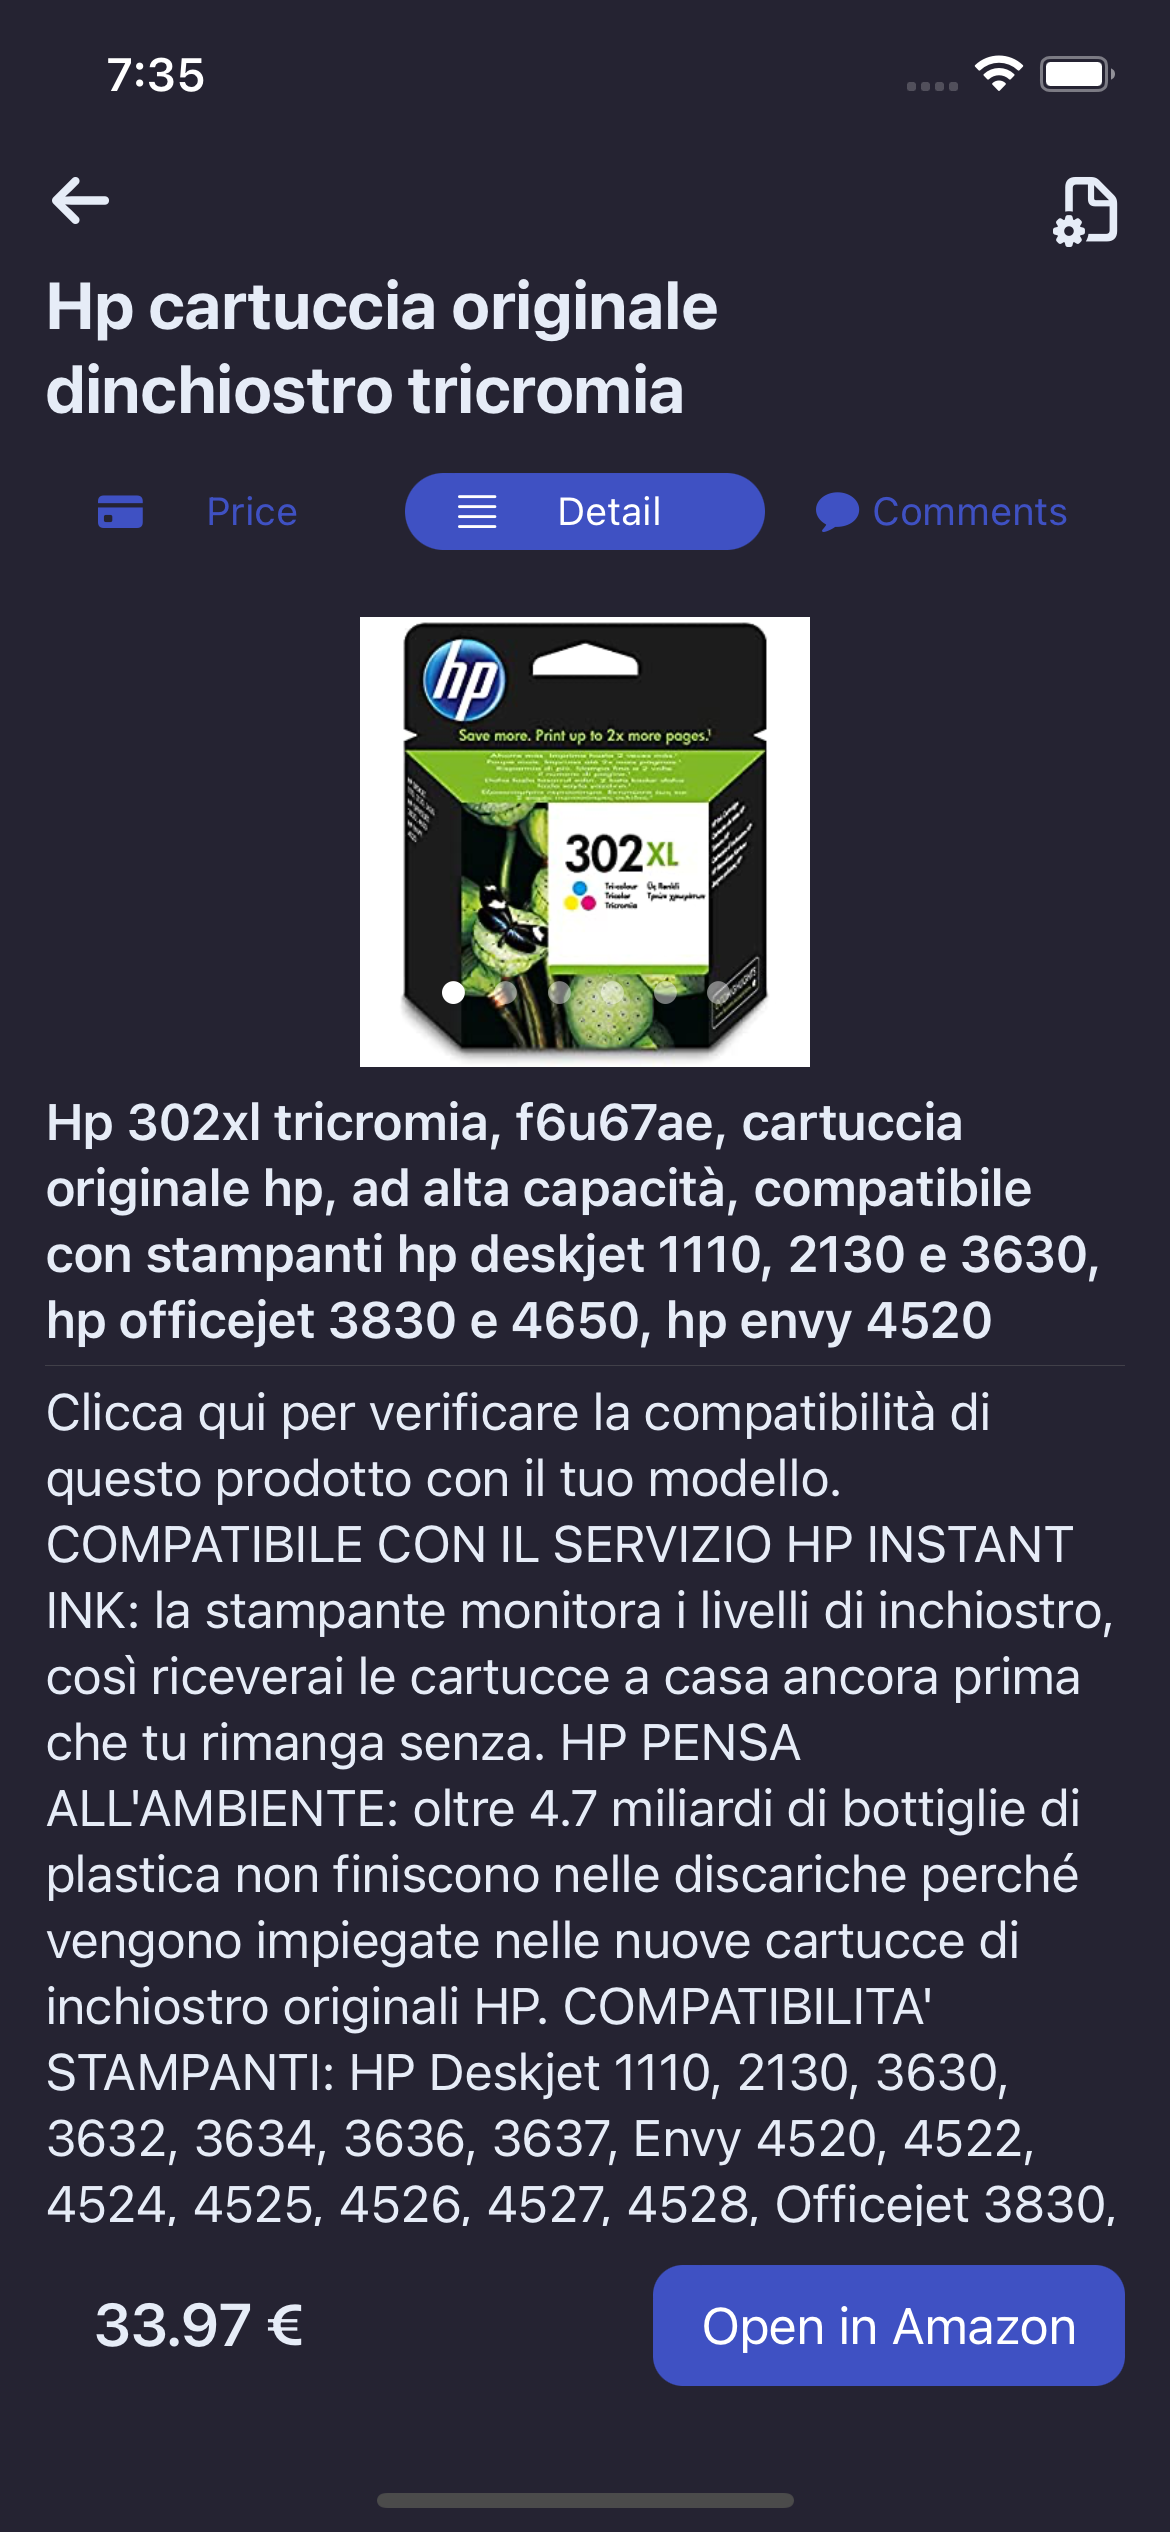
\includegraphics[scale=0.15]{images/interfaces/detail_product_screen.png}
        \caption{Detail product screen}
        \label{fig:detail_product_screen}
\end{figure}
\FloatBarrier
This is the view containing the detail of a product (fig: \ref{fig:detail_product_screen}). From here the user can browse all the photos of the product (full screen mode by clicking on an image), the full name, the category and the description.\\\\

The comments of the product are comment inserted by the user of myAPTracker and not comments of Amazon.
\begin{figure}[h!]
        \centering
        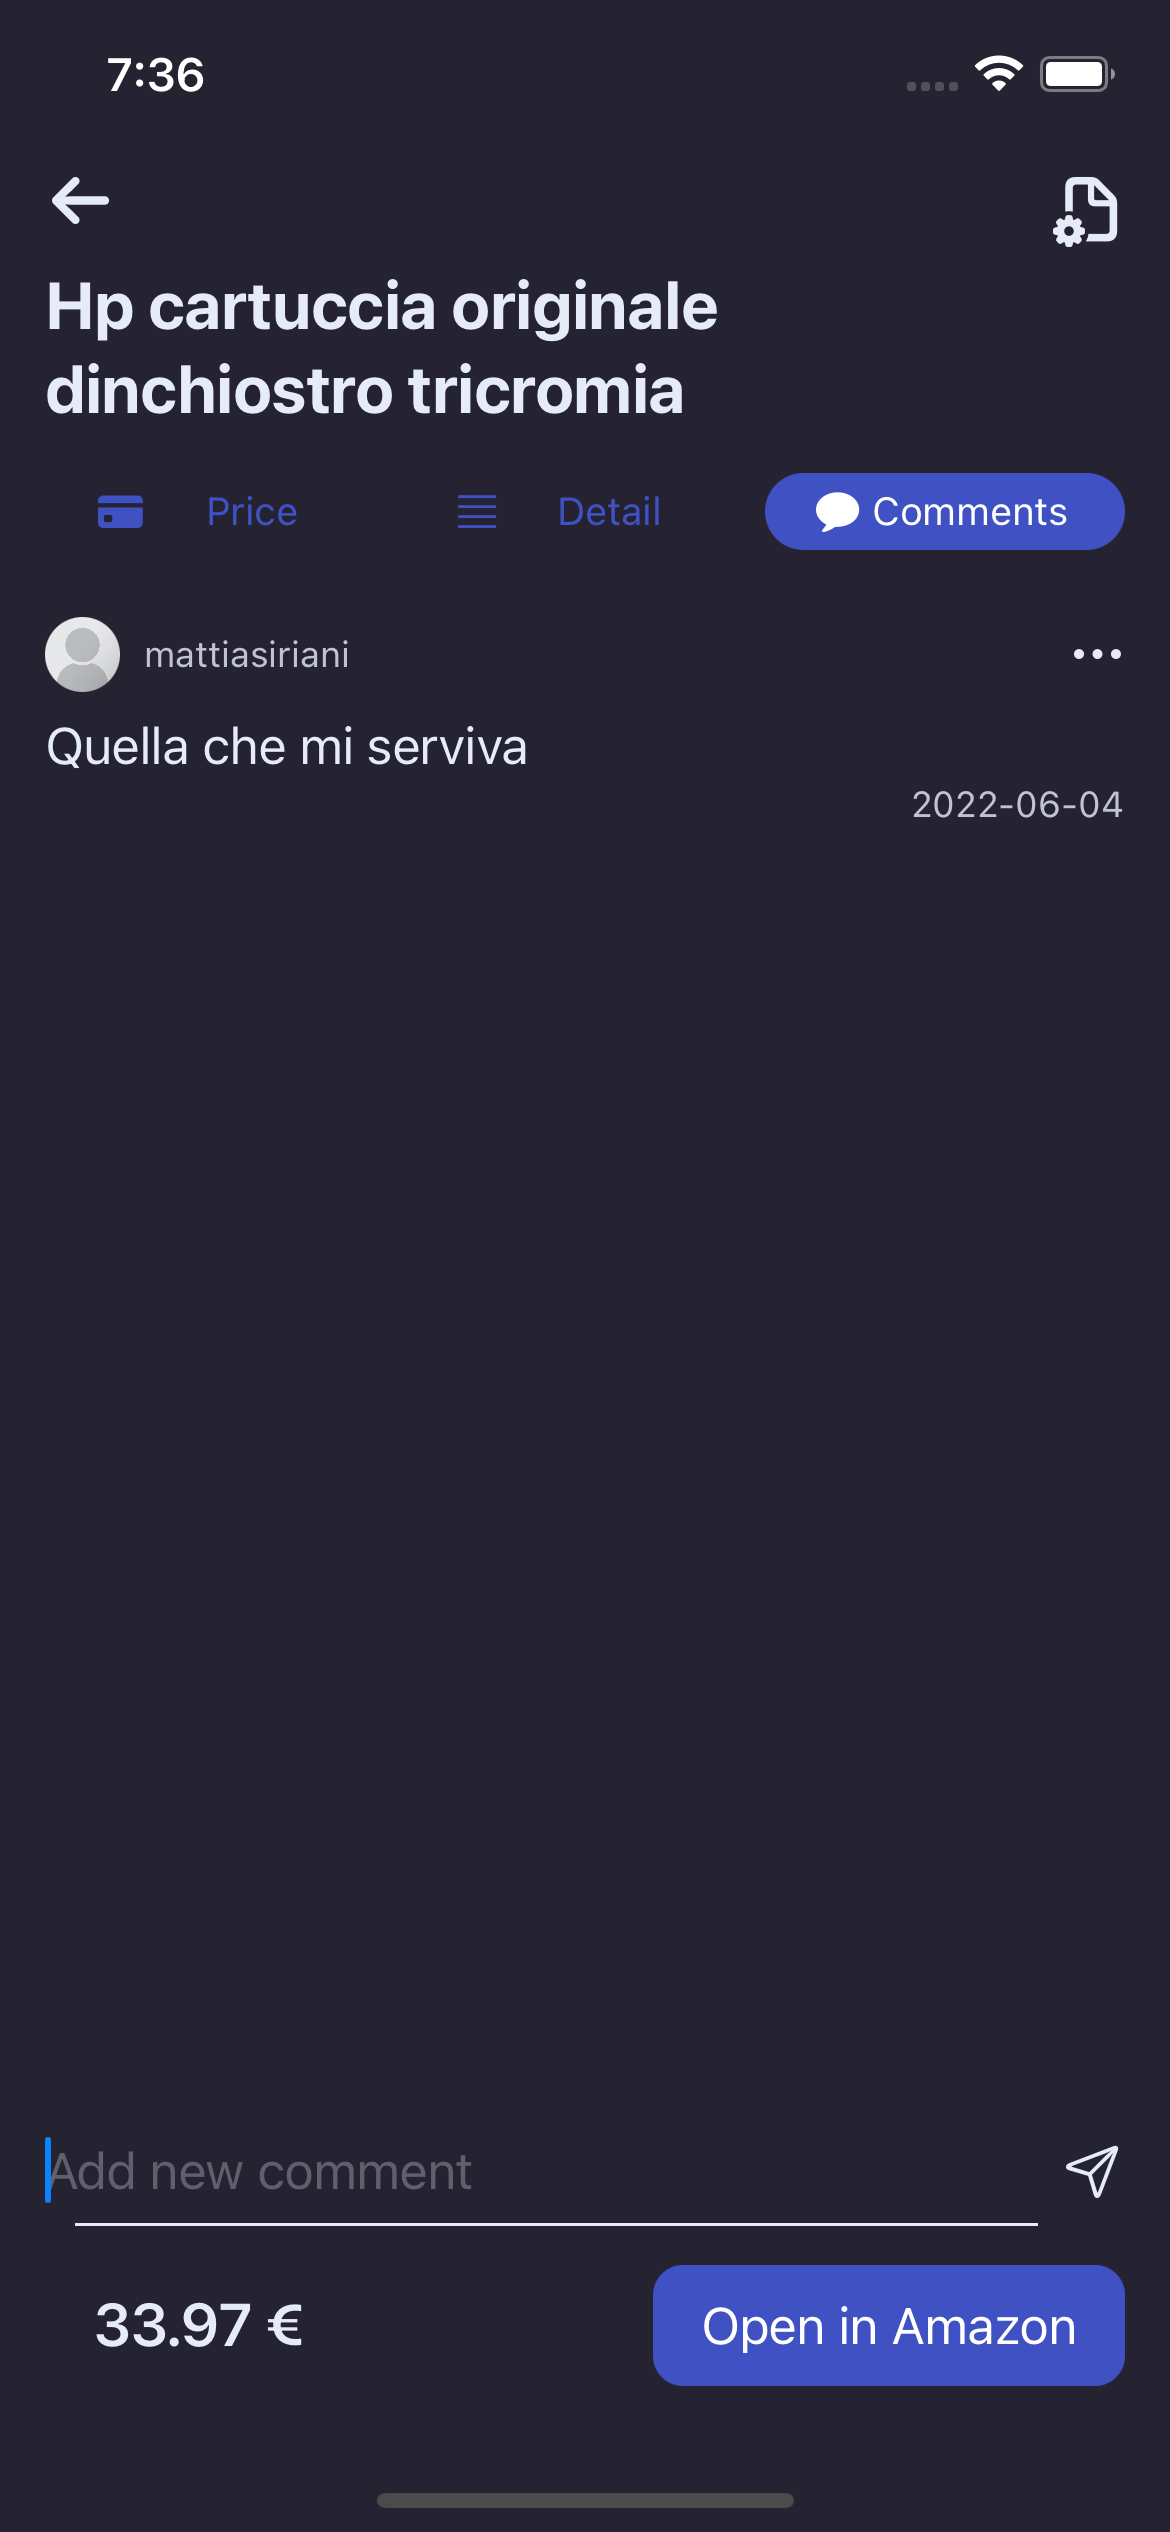
\includegraphics[scale=0.15]{images/interfaces/comments_product_screen.png}
        \caption{Comments product screen}
        \label{fig:comments_product_screen}
\end{figure}
\FloatBarrier
This is the view containing all the comments that a product has ever received (fig: \ref{fig:comments_product_screen}). From here the user can see the comments of the product or adding a comment itself.
Finally, a user can delete its comment, after he post them.
\\\\

The next screen are the iPad screen for the products and are put in a separate section, because here is not possible to switch between three sections, but only between two. In fact the price view is always visible on the left while the user can switch between detail and comments on the right.

\begin{figure}[h!]
        \centering
        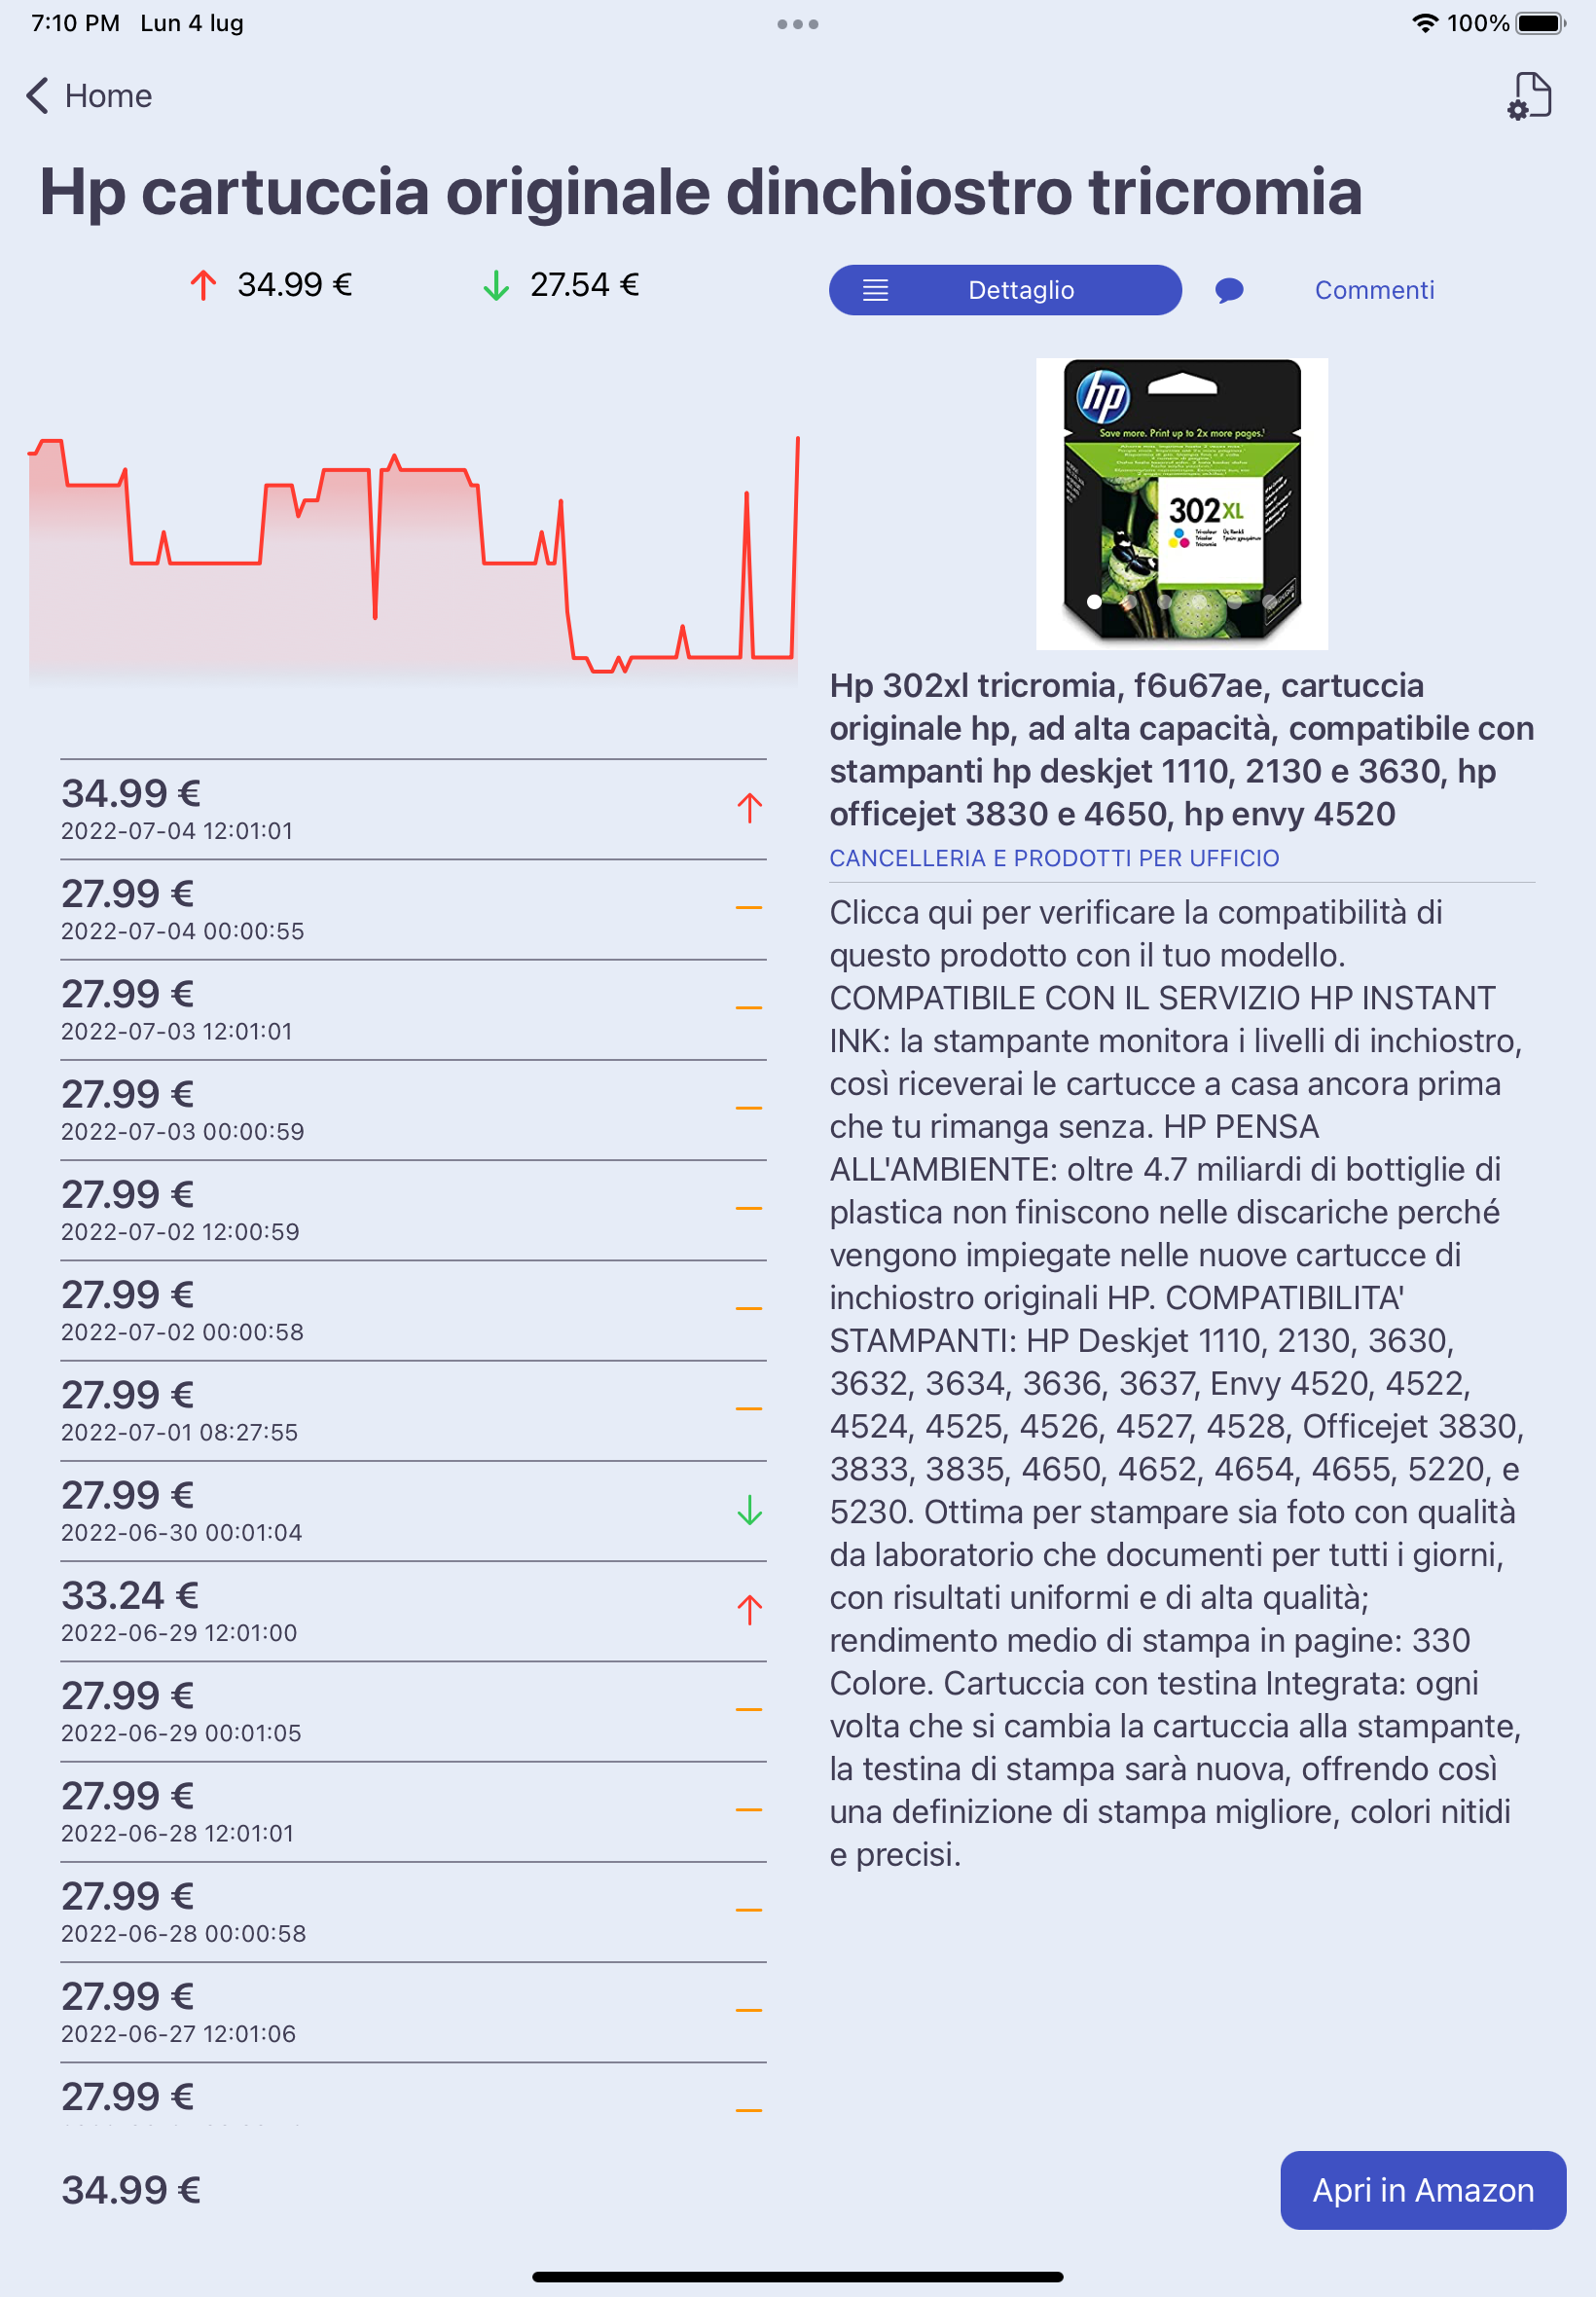
\includegraphics[scale=0.15]{images/interfaces/product_and_detail_ipad.png}
        \caption{Product and detail screen}
        \label{fig:product_and_detail_ipad}
\end{figure}
\FloatBarrier

\begin{figure}[h!]
        \centering
        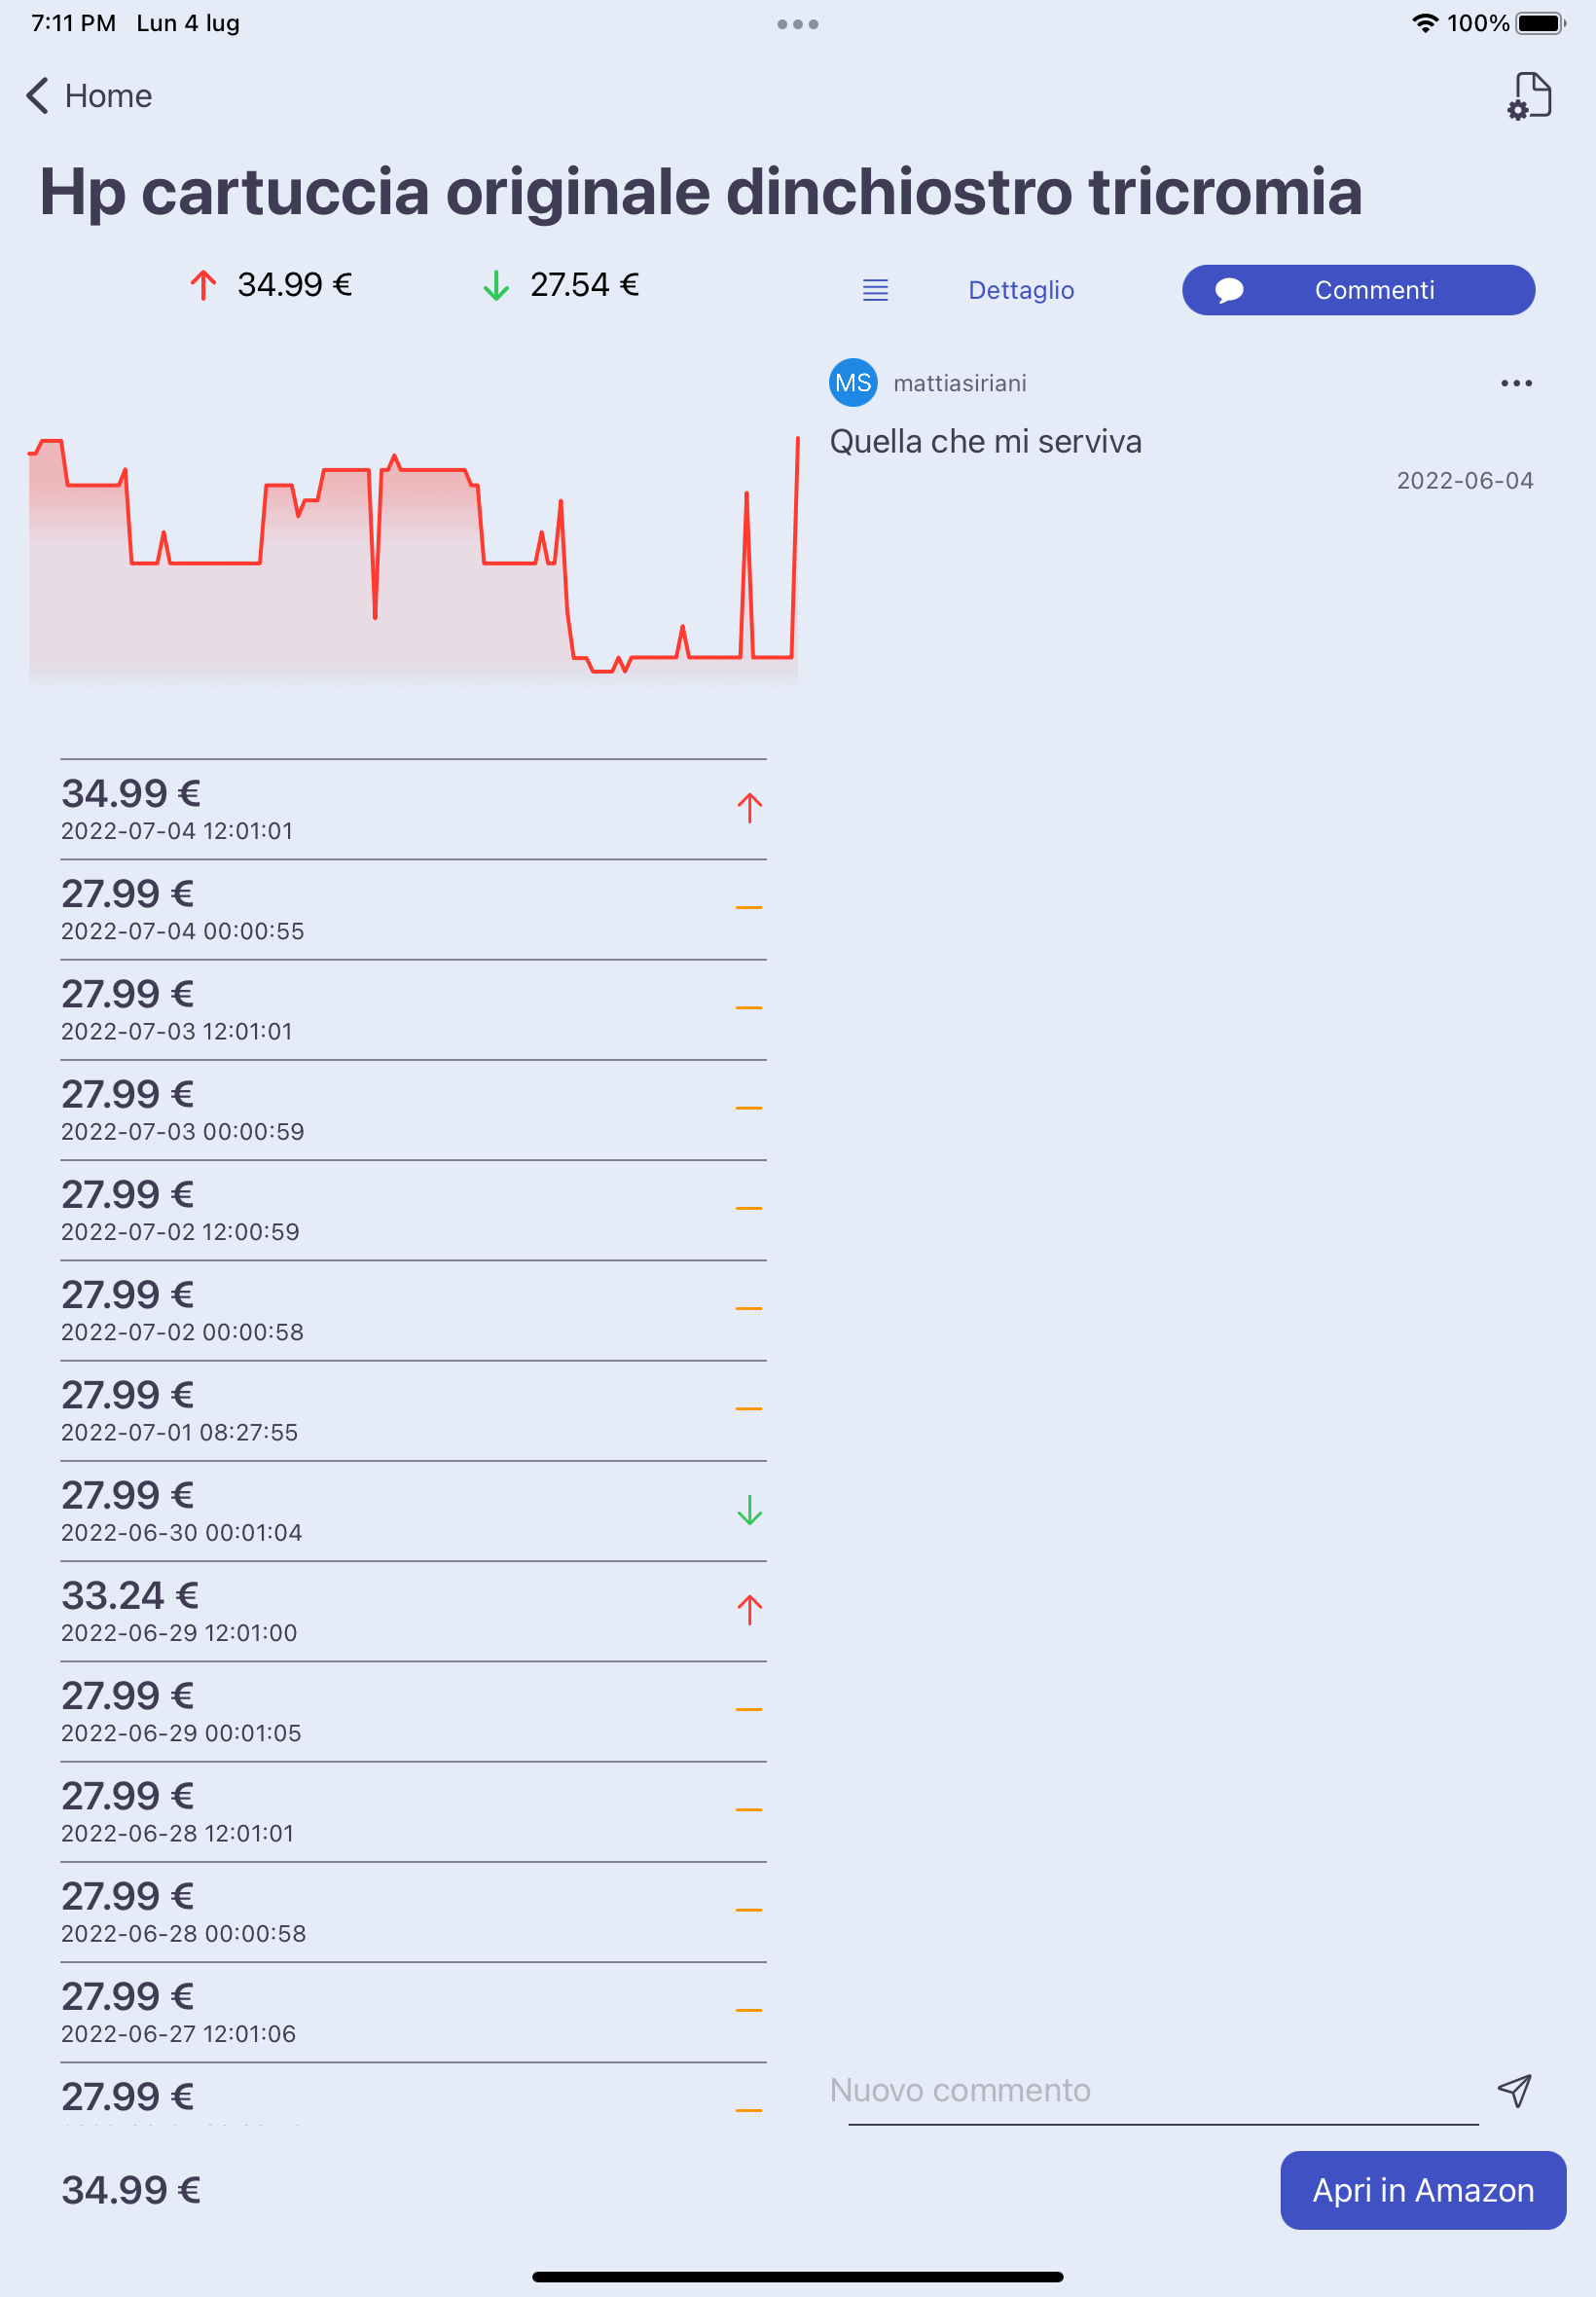
\includegraphics[scale=0.15]{images/interfaces/product_and_comment_ipad.png}
        \caption{Product and screen}
        \label{fig:product_and_comment_ipad}
\end{figure}
\FloatBarrier


The following screen represents the tracking settings. Here, the user can choose if receive the notification about a price drop as well as a notification about a new comment posted in the product page. In the next pages we will explain better the available options about notification for products since for comments it is only possible to enable or disable them:




\begin{figure}[h!]
        \centering
        \begin{subfigure}[b]{0.3\textwidth}
            \centering
            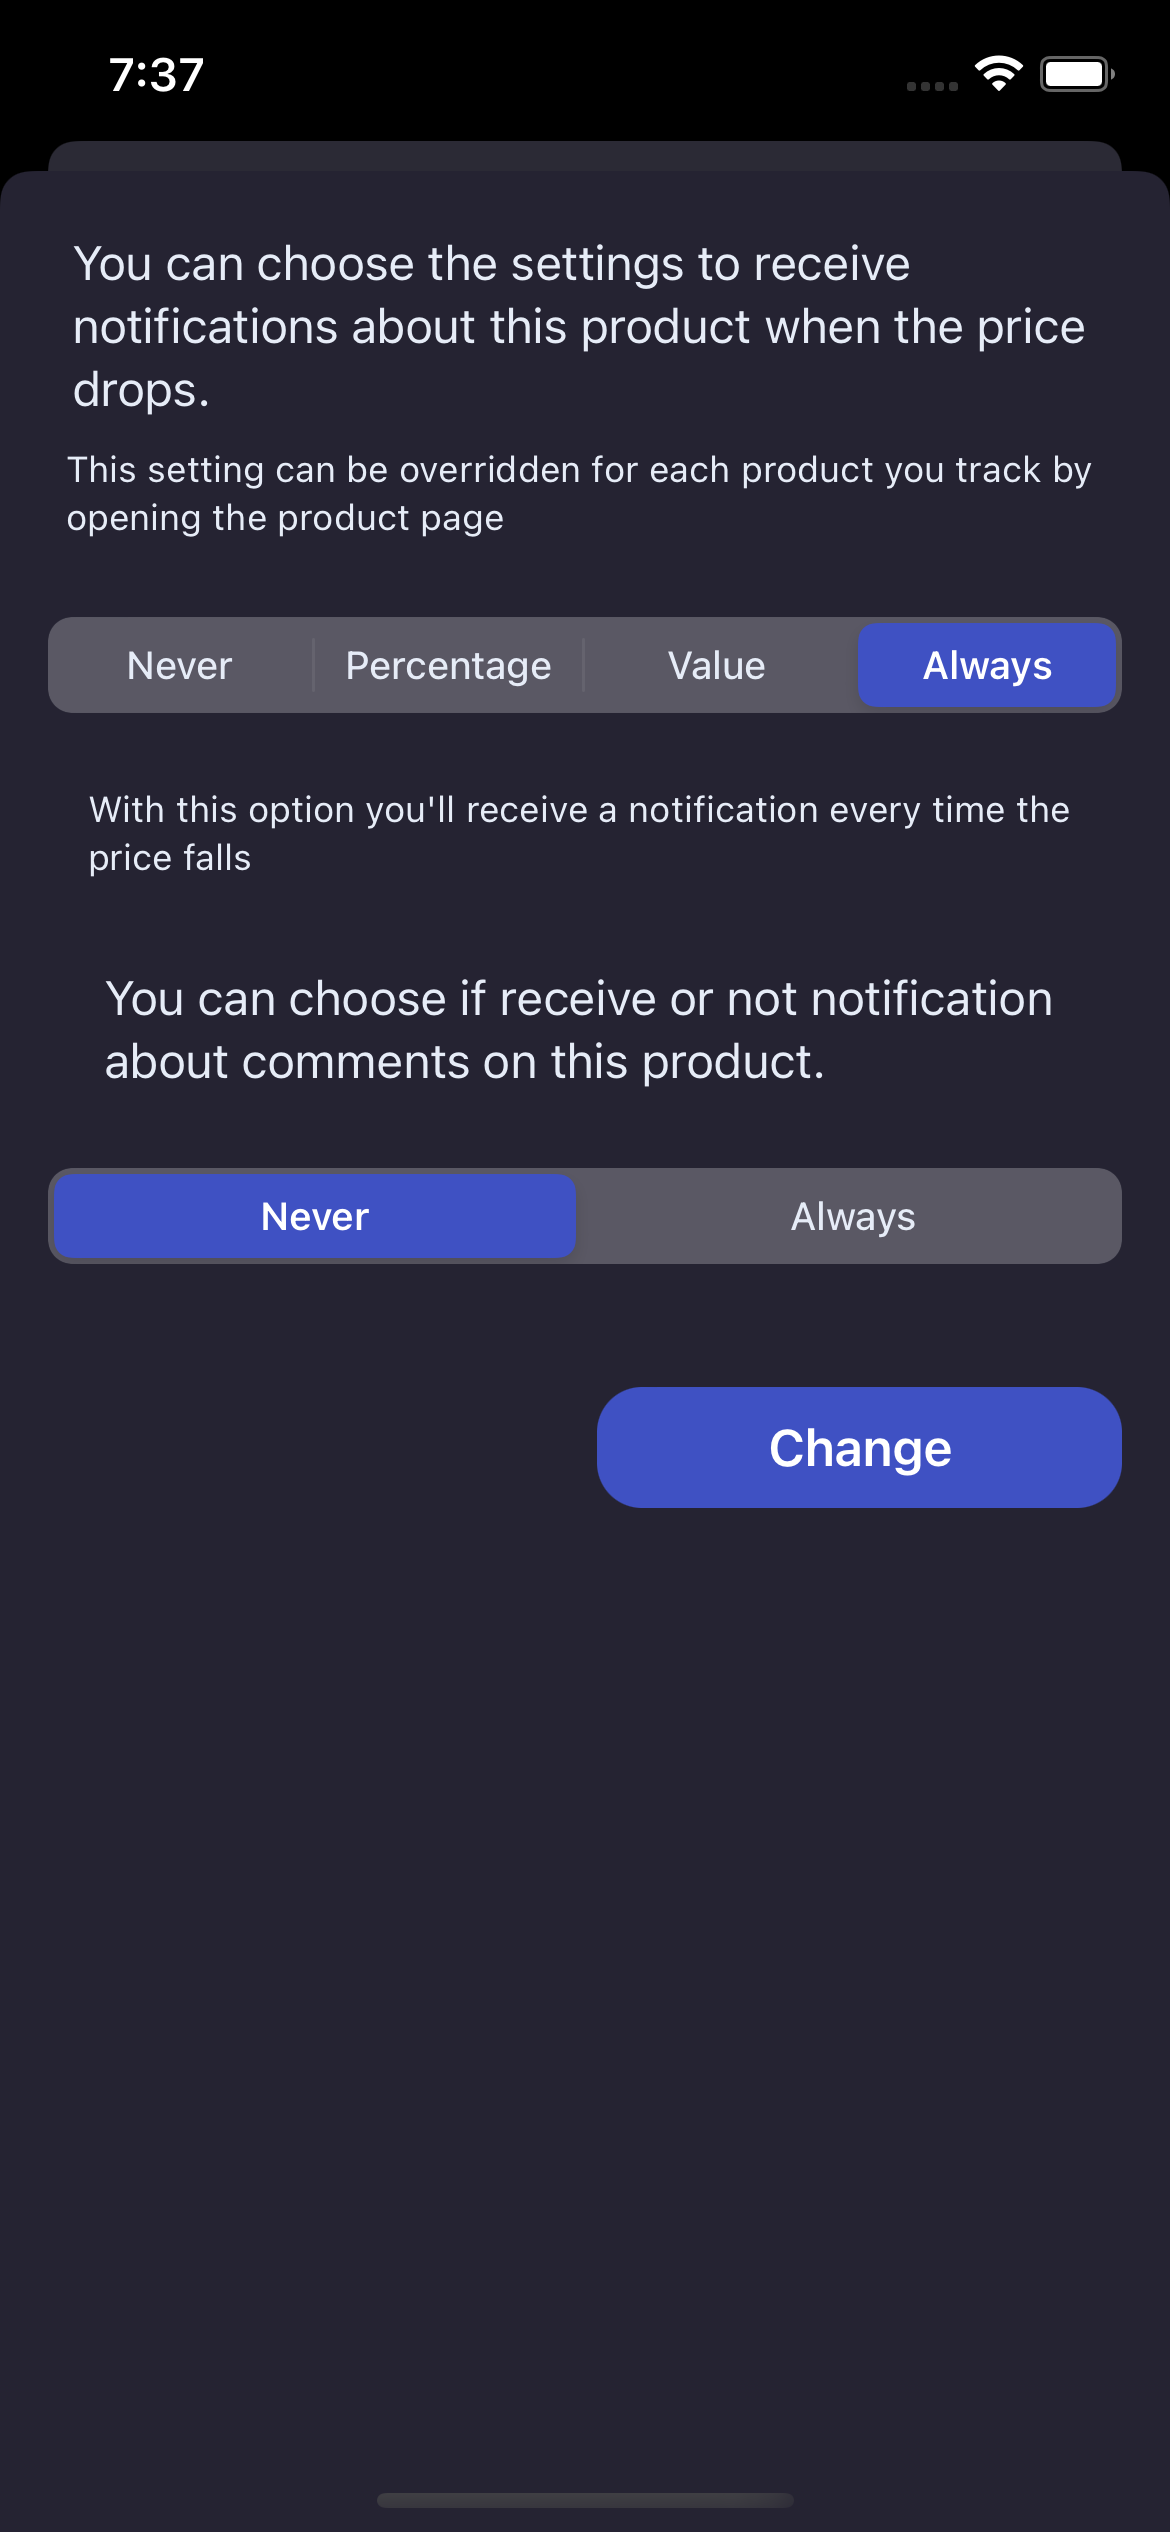
\includegraphics[width=\textwidth]{images/interfaces/always_never_notification_screen.png}
            \caption{iPhone}
            \label{fig:always_never_notification_screen_iphone}
        \end{subfigure}
        \begin{subfigure}[b]{0.45\textwidth}
            \centering
            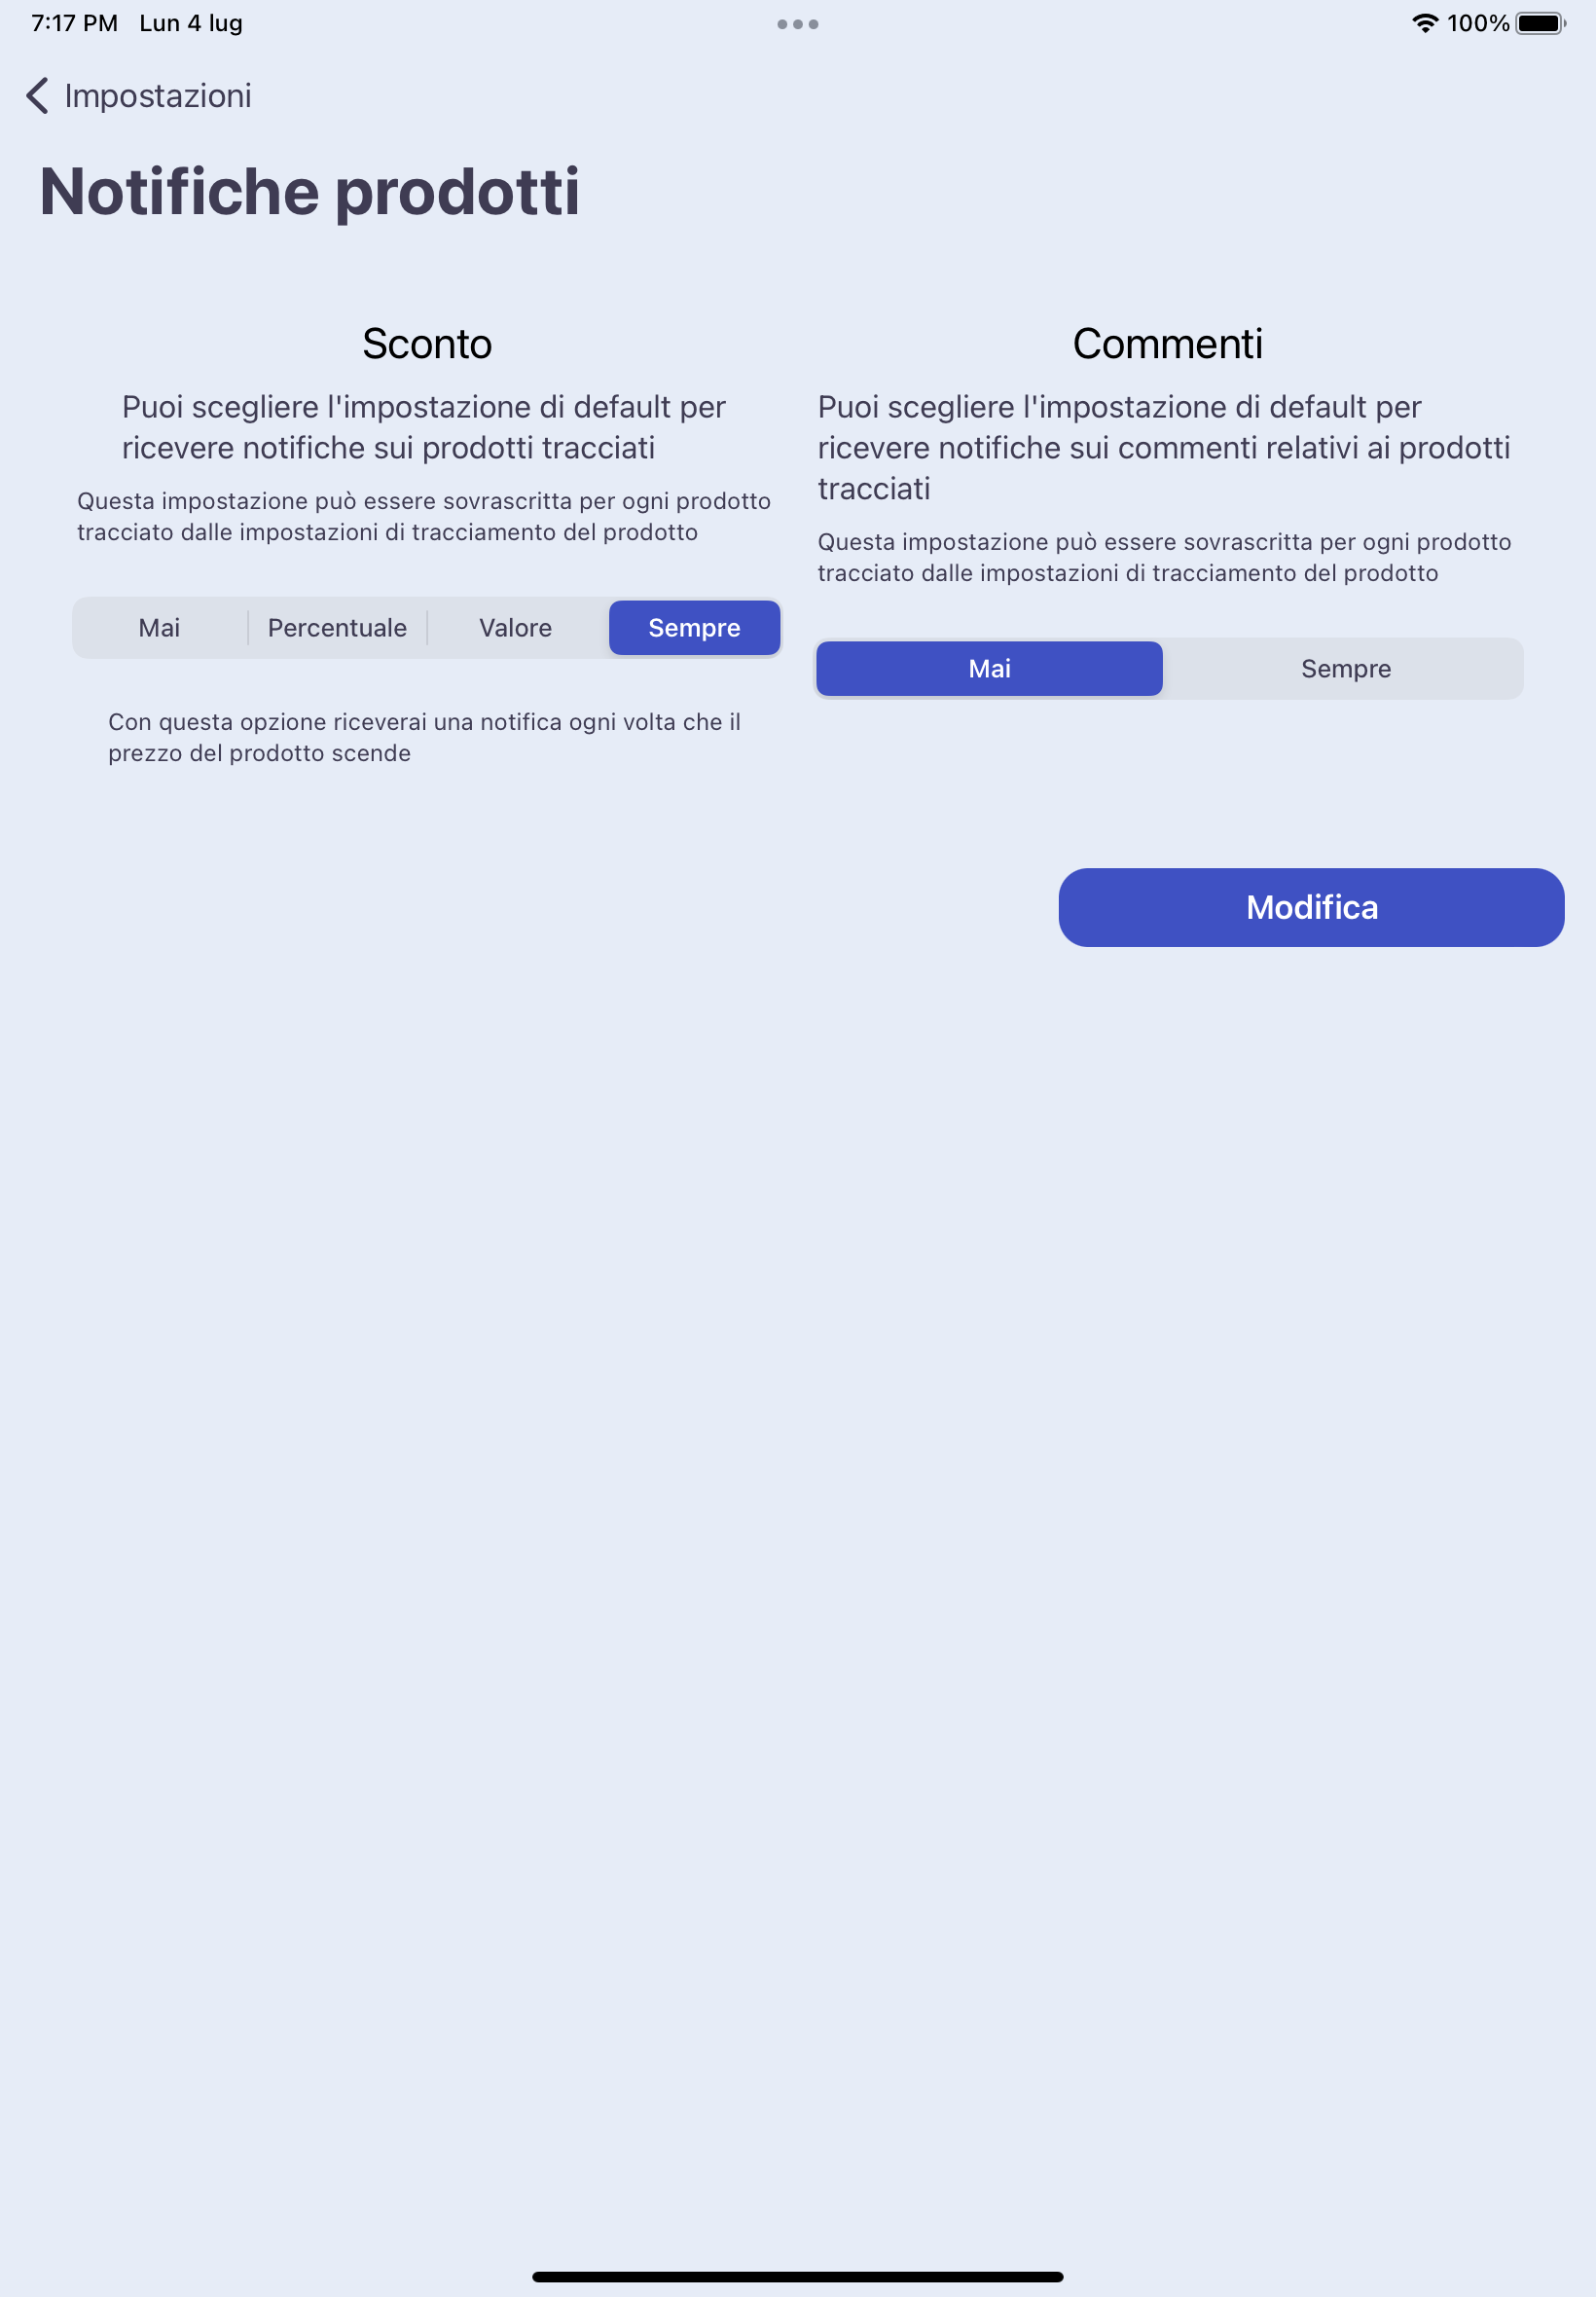
\includegraphics[width=\textwidth]{images/interfaces/always_never_notification_screen_ipad.png}
            \caption{iPad}
            \label{fig:always_never_notification_screen_ipad}
        \end{subfigure}
         \caption{Receive notification always or never screen}
        \label{fig:always_never_notification_screen}
\end{figure}
\FloatBarrier
In figure \ref{fig:always_never_notification_screen} the "always" option is selected, no further options are available (as well as "never") since a notification is sent any time the price falls down.

\begin{figure}[h!]
        \centering
        \begin{subfigure}[b]{0.3\textwidth}
            \centering
            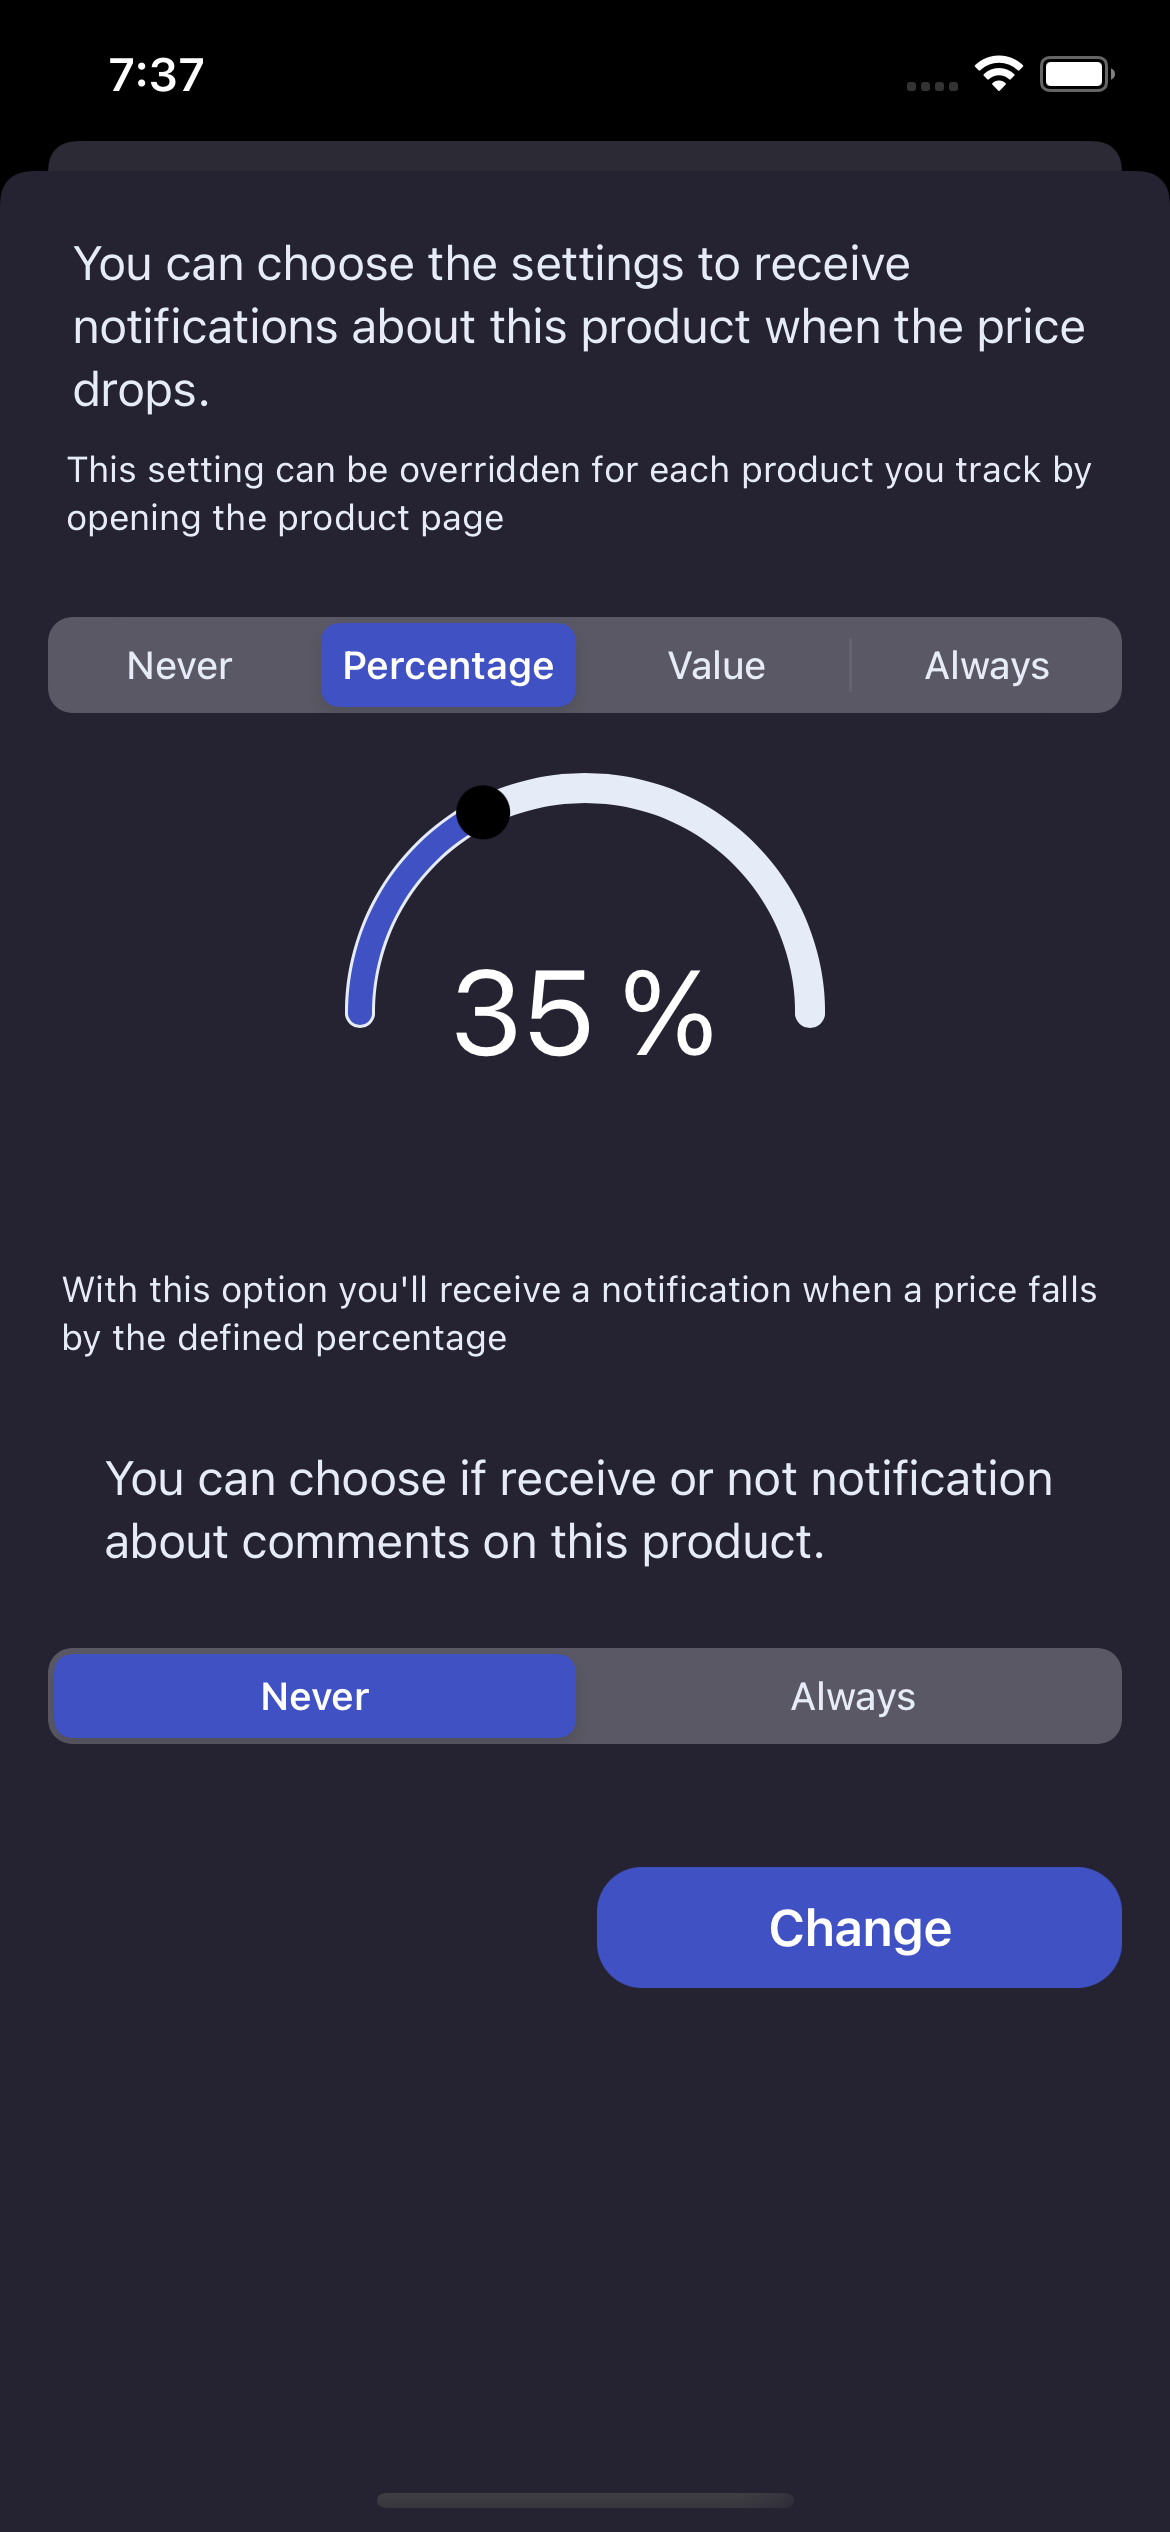
\includegraphics[width=\textwidth]{images/interfaces/percentage_notification_screen.png}
            \caption{iPhone}
            \label{fig:percentage_notification_screen_iphone}
        \end{subfigure}
        \begin{subfigure}[b]{0.45\textwidth}
            \centering
            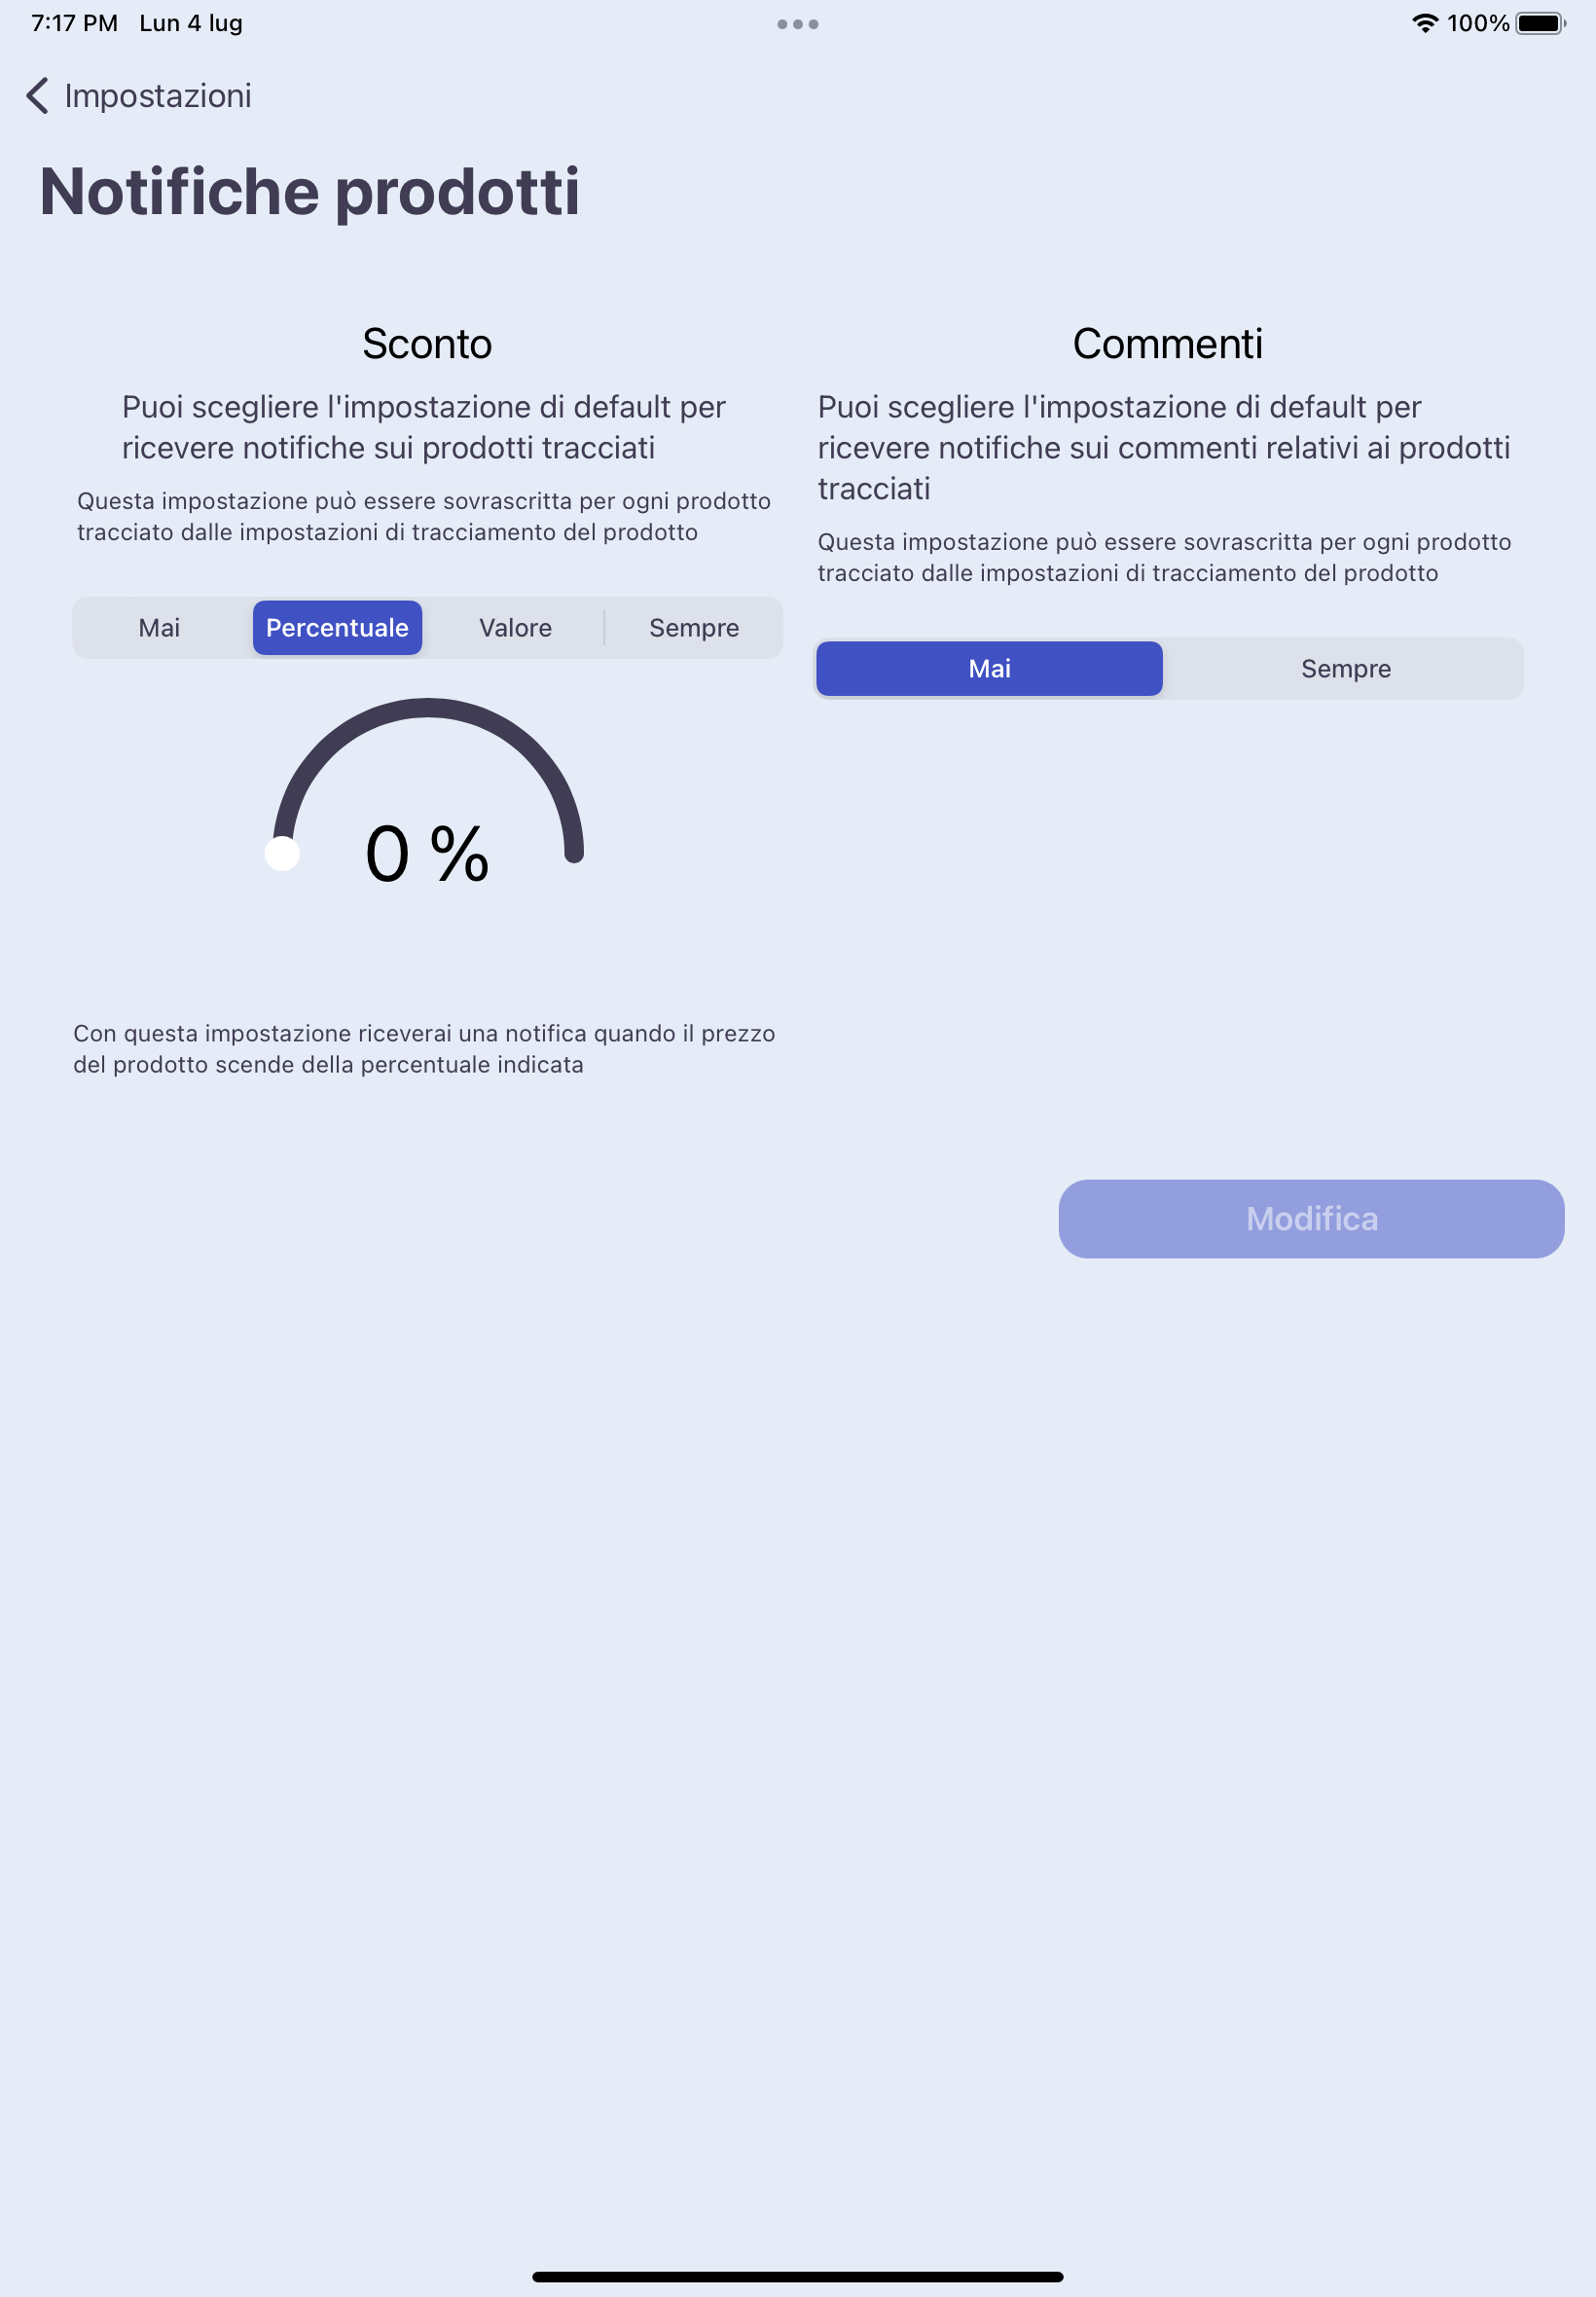
\includegraphics[width=\textwidth]{images/interfaces/percentage_notification_screen_ipad.png}
            \caption{iPad}
            \label{fig:percentage_notification_screen_ipad}
        \end{subfigure}
         \caption{Receive notification from a percentage of the actual price screen}
        \label{fig:percentage_notification_screen}
\end{figure}
\FloatBarrier
In figure \ref{fig:percentage_notification_screen} we can see the "percentage" setting, the half circle slider let the user to set the percentage value under which the notification is sent. For example, if the user set the value to 35\% the notification is delivered by the system only if the difference between the last and the available price when the user starts tracking the product is grater or equals of the 35\%.
\\
\begin{equation}
    (\frac{newPrice - targetPrice}{targetPrice}*100)*(-1) \geq settingValue
\end{equation}
Since in the interface the percentage is set as positive, we multiply the drop percentage for $-1$ in order the consider a discount as positive.

\begin{figure}[h!]
        \centering
        \begin{subfigure}[b]{0.3\textwidth}
            \centering
            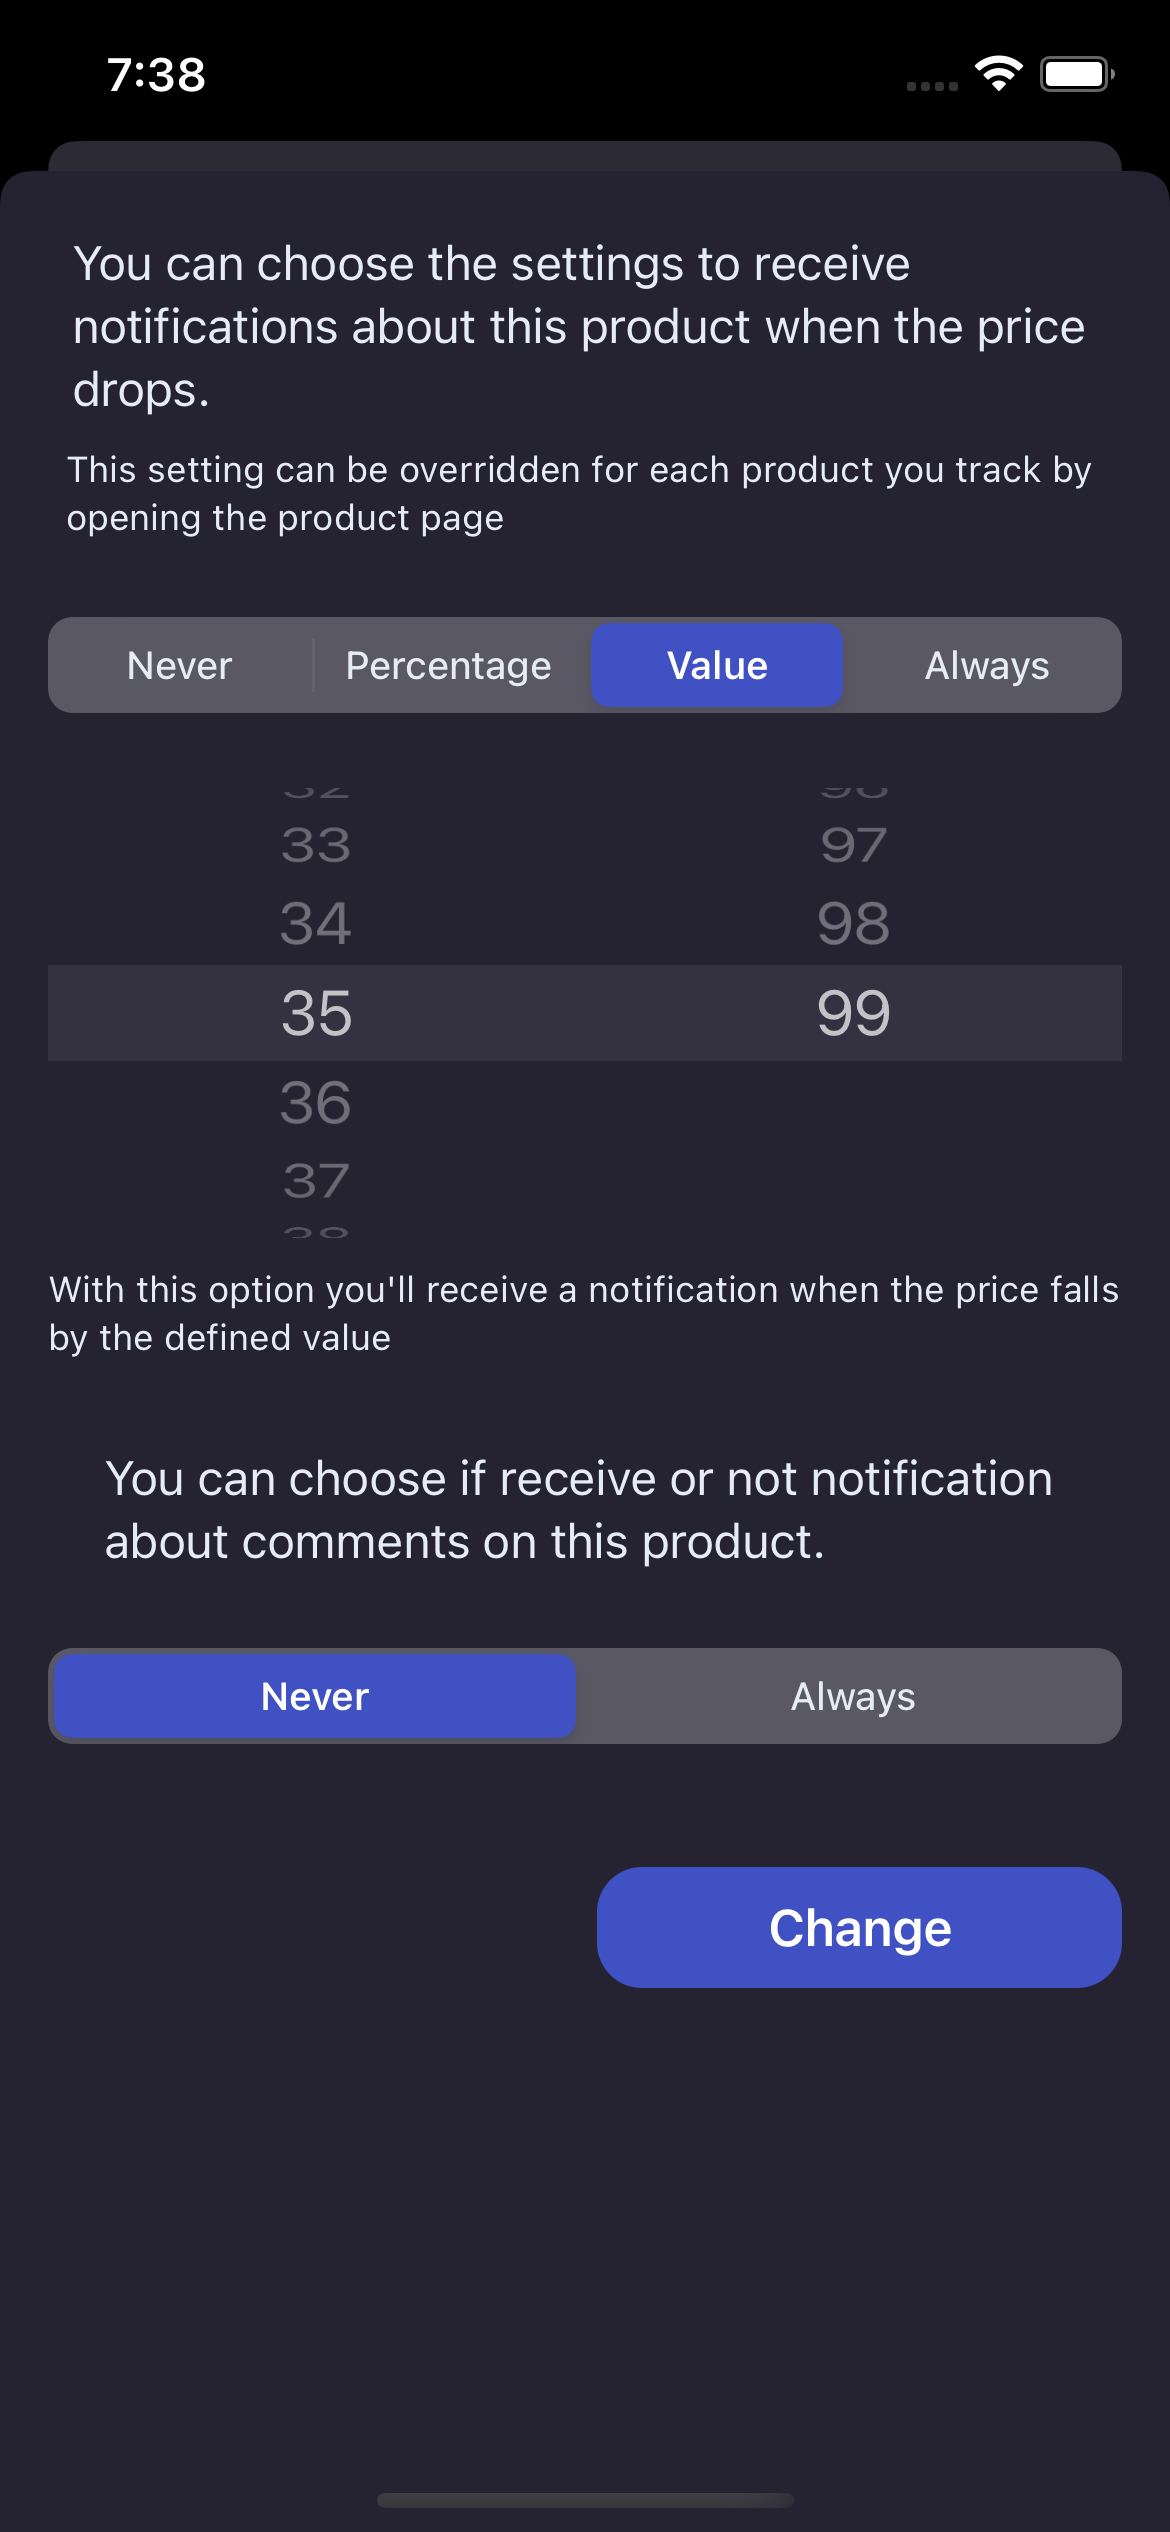
\includegraphics[width=\textwidth]{images/interfaces/value_notification_screen.png}
            \caption{iPhone}
            \label{fig:value_notification_screen_iphone}
        \end{subfigure}
        \begin{subfigure}[b]{0.45\textwidth}
            \centering
            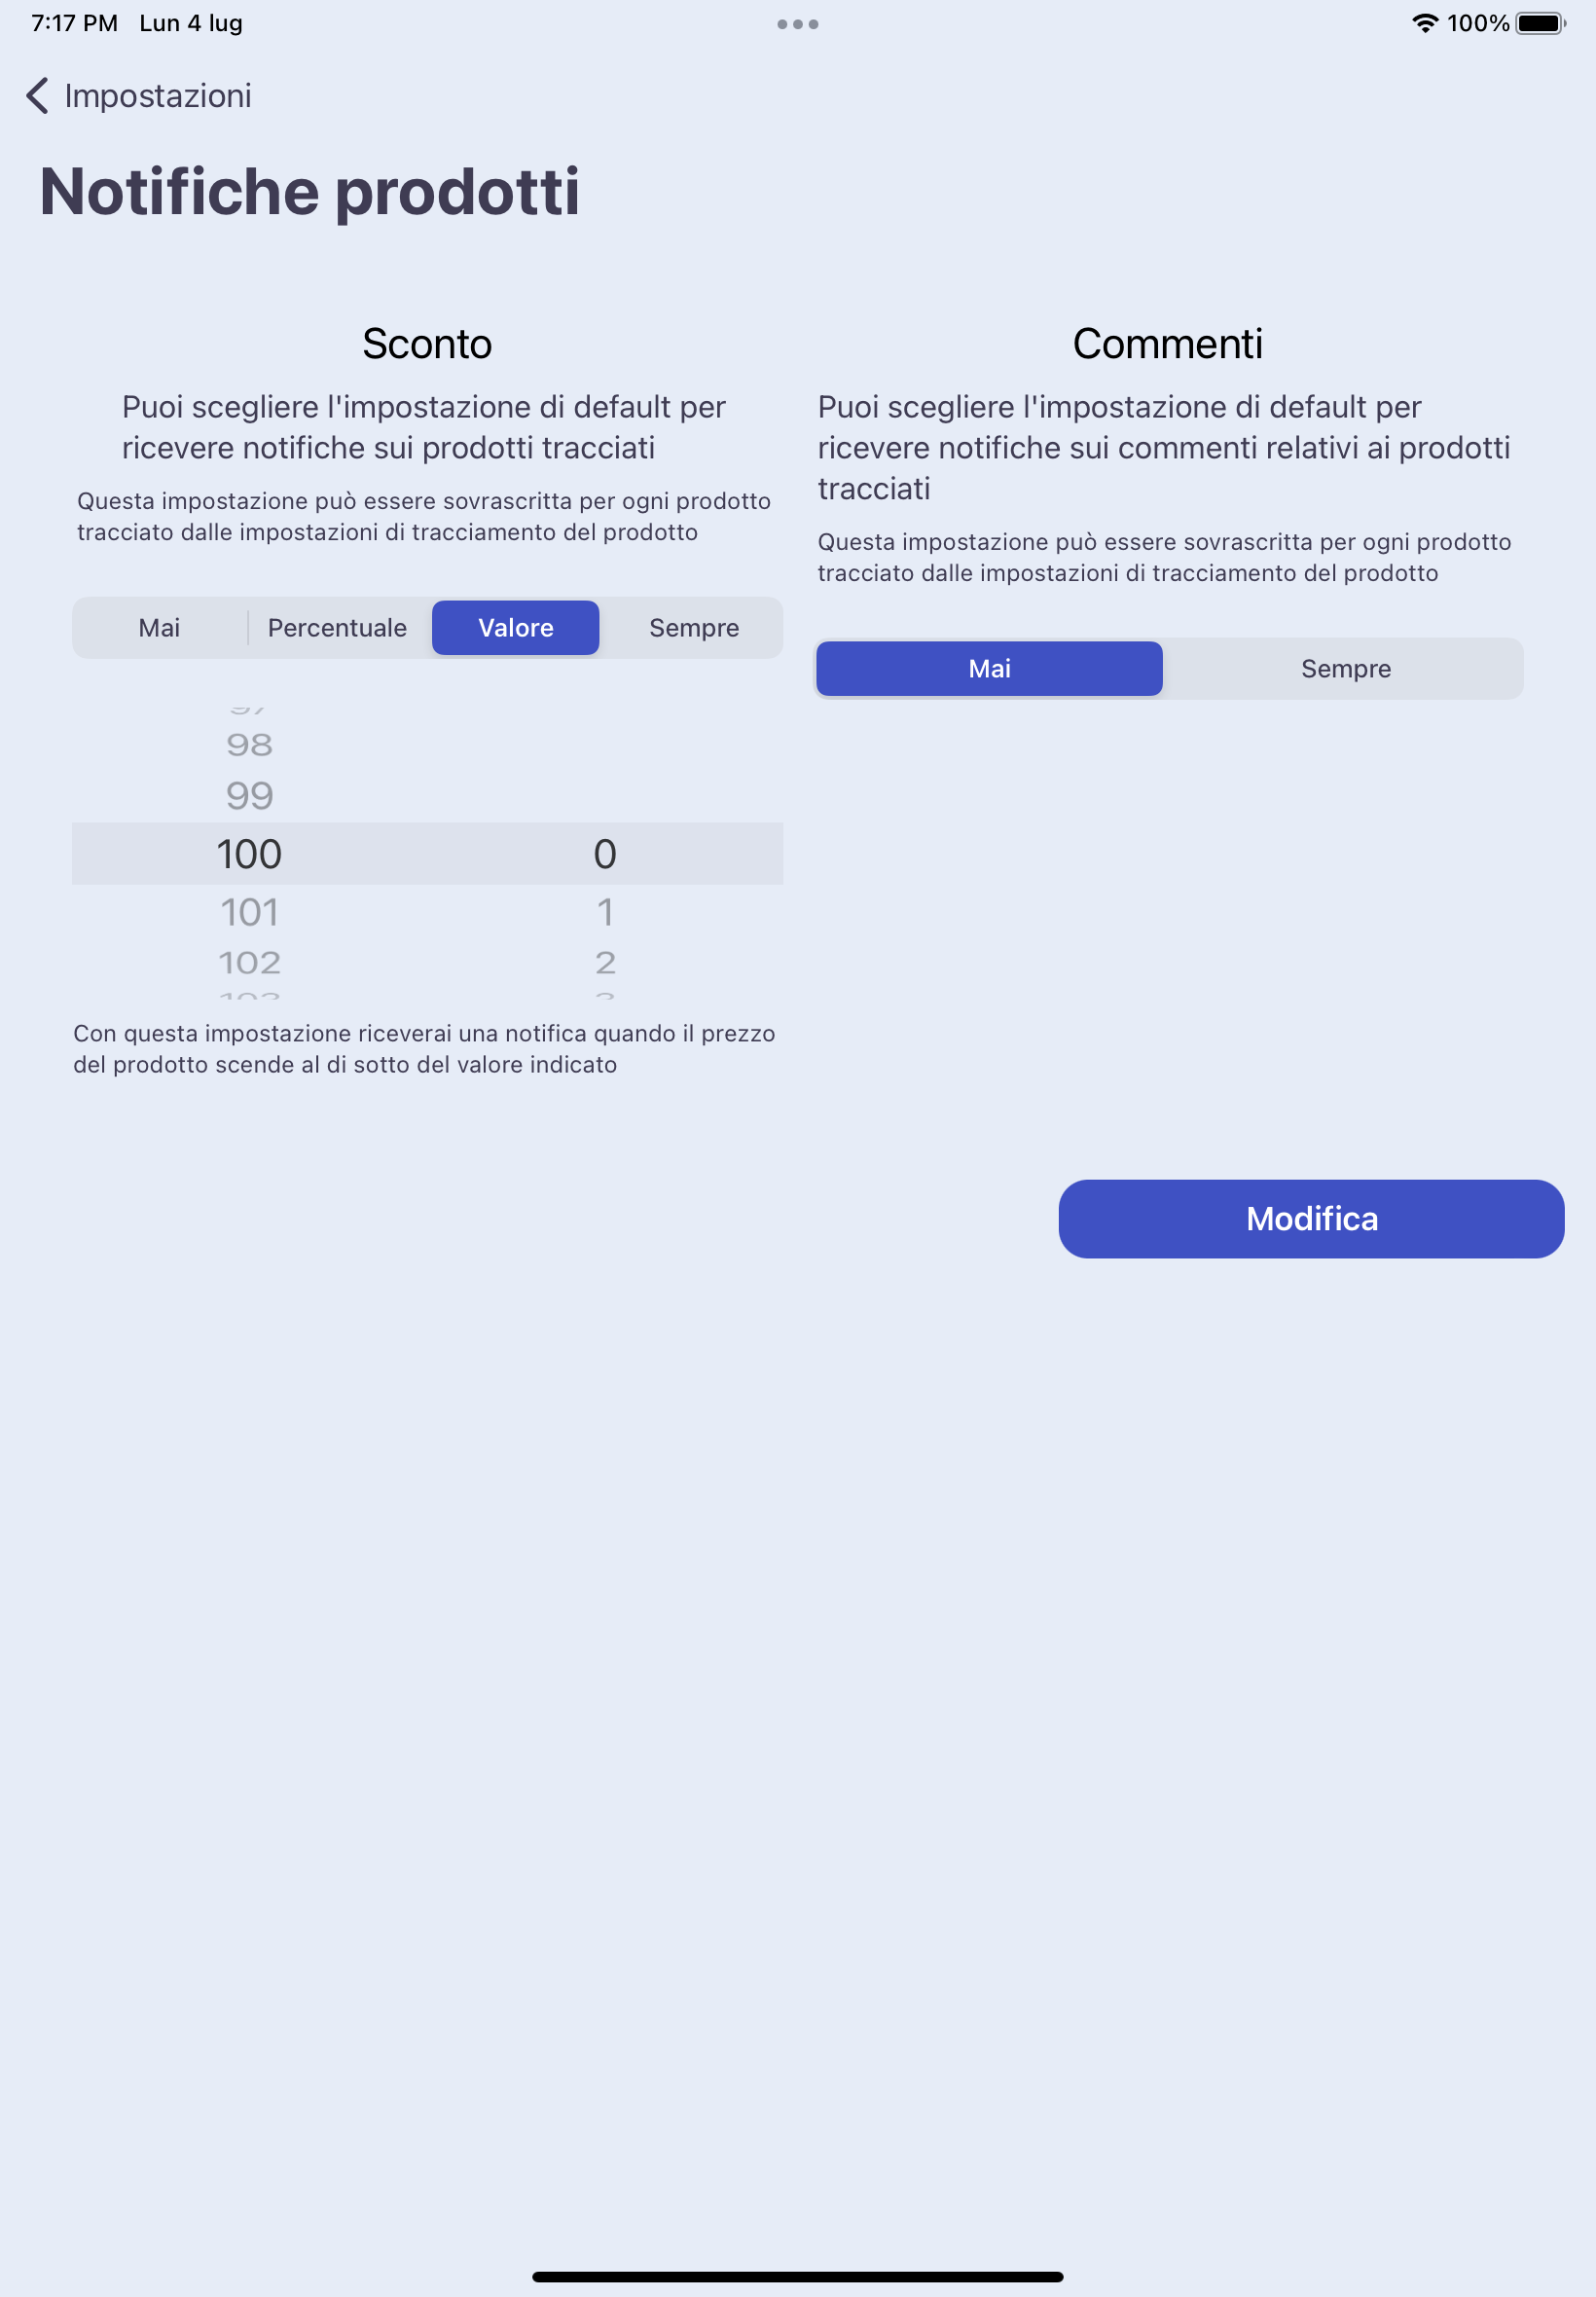
\includegraphics[width=\textwidth]{images/interfaces/value_notification_screen_ipad.png}
            \caption{iPad}
            \label{fig:value_notification_screen_ipad}
        \end{subfigure}
         \caption{Receive notification if product is under a value screen}
        \label{fig:value_notification_screen}
\end{figure}
\FloatBarrier
Finally in figure \ref{fig:value_notification_screen} we can see how the "value" option looks like. In this case the user can set a target price and when the product price in less or equal the target the user will be notified.
\\\\

\begin{figure}[h!]
        \centering
        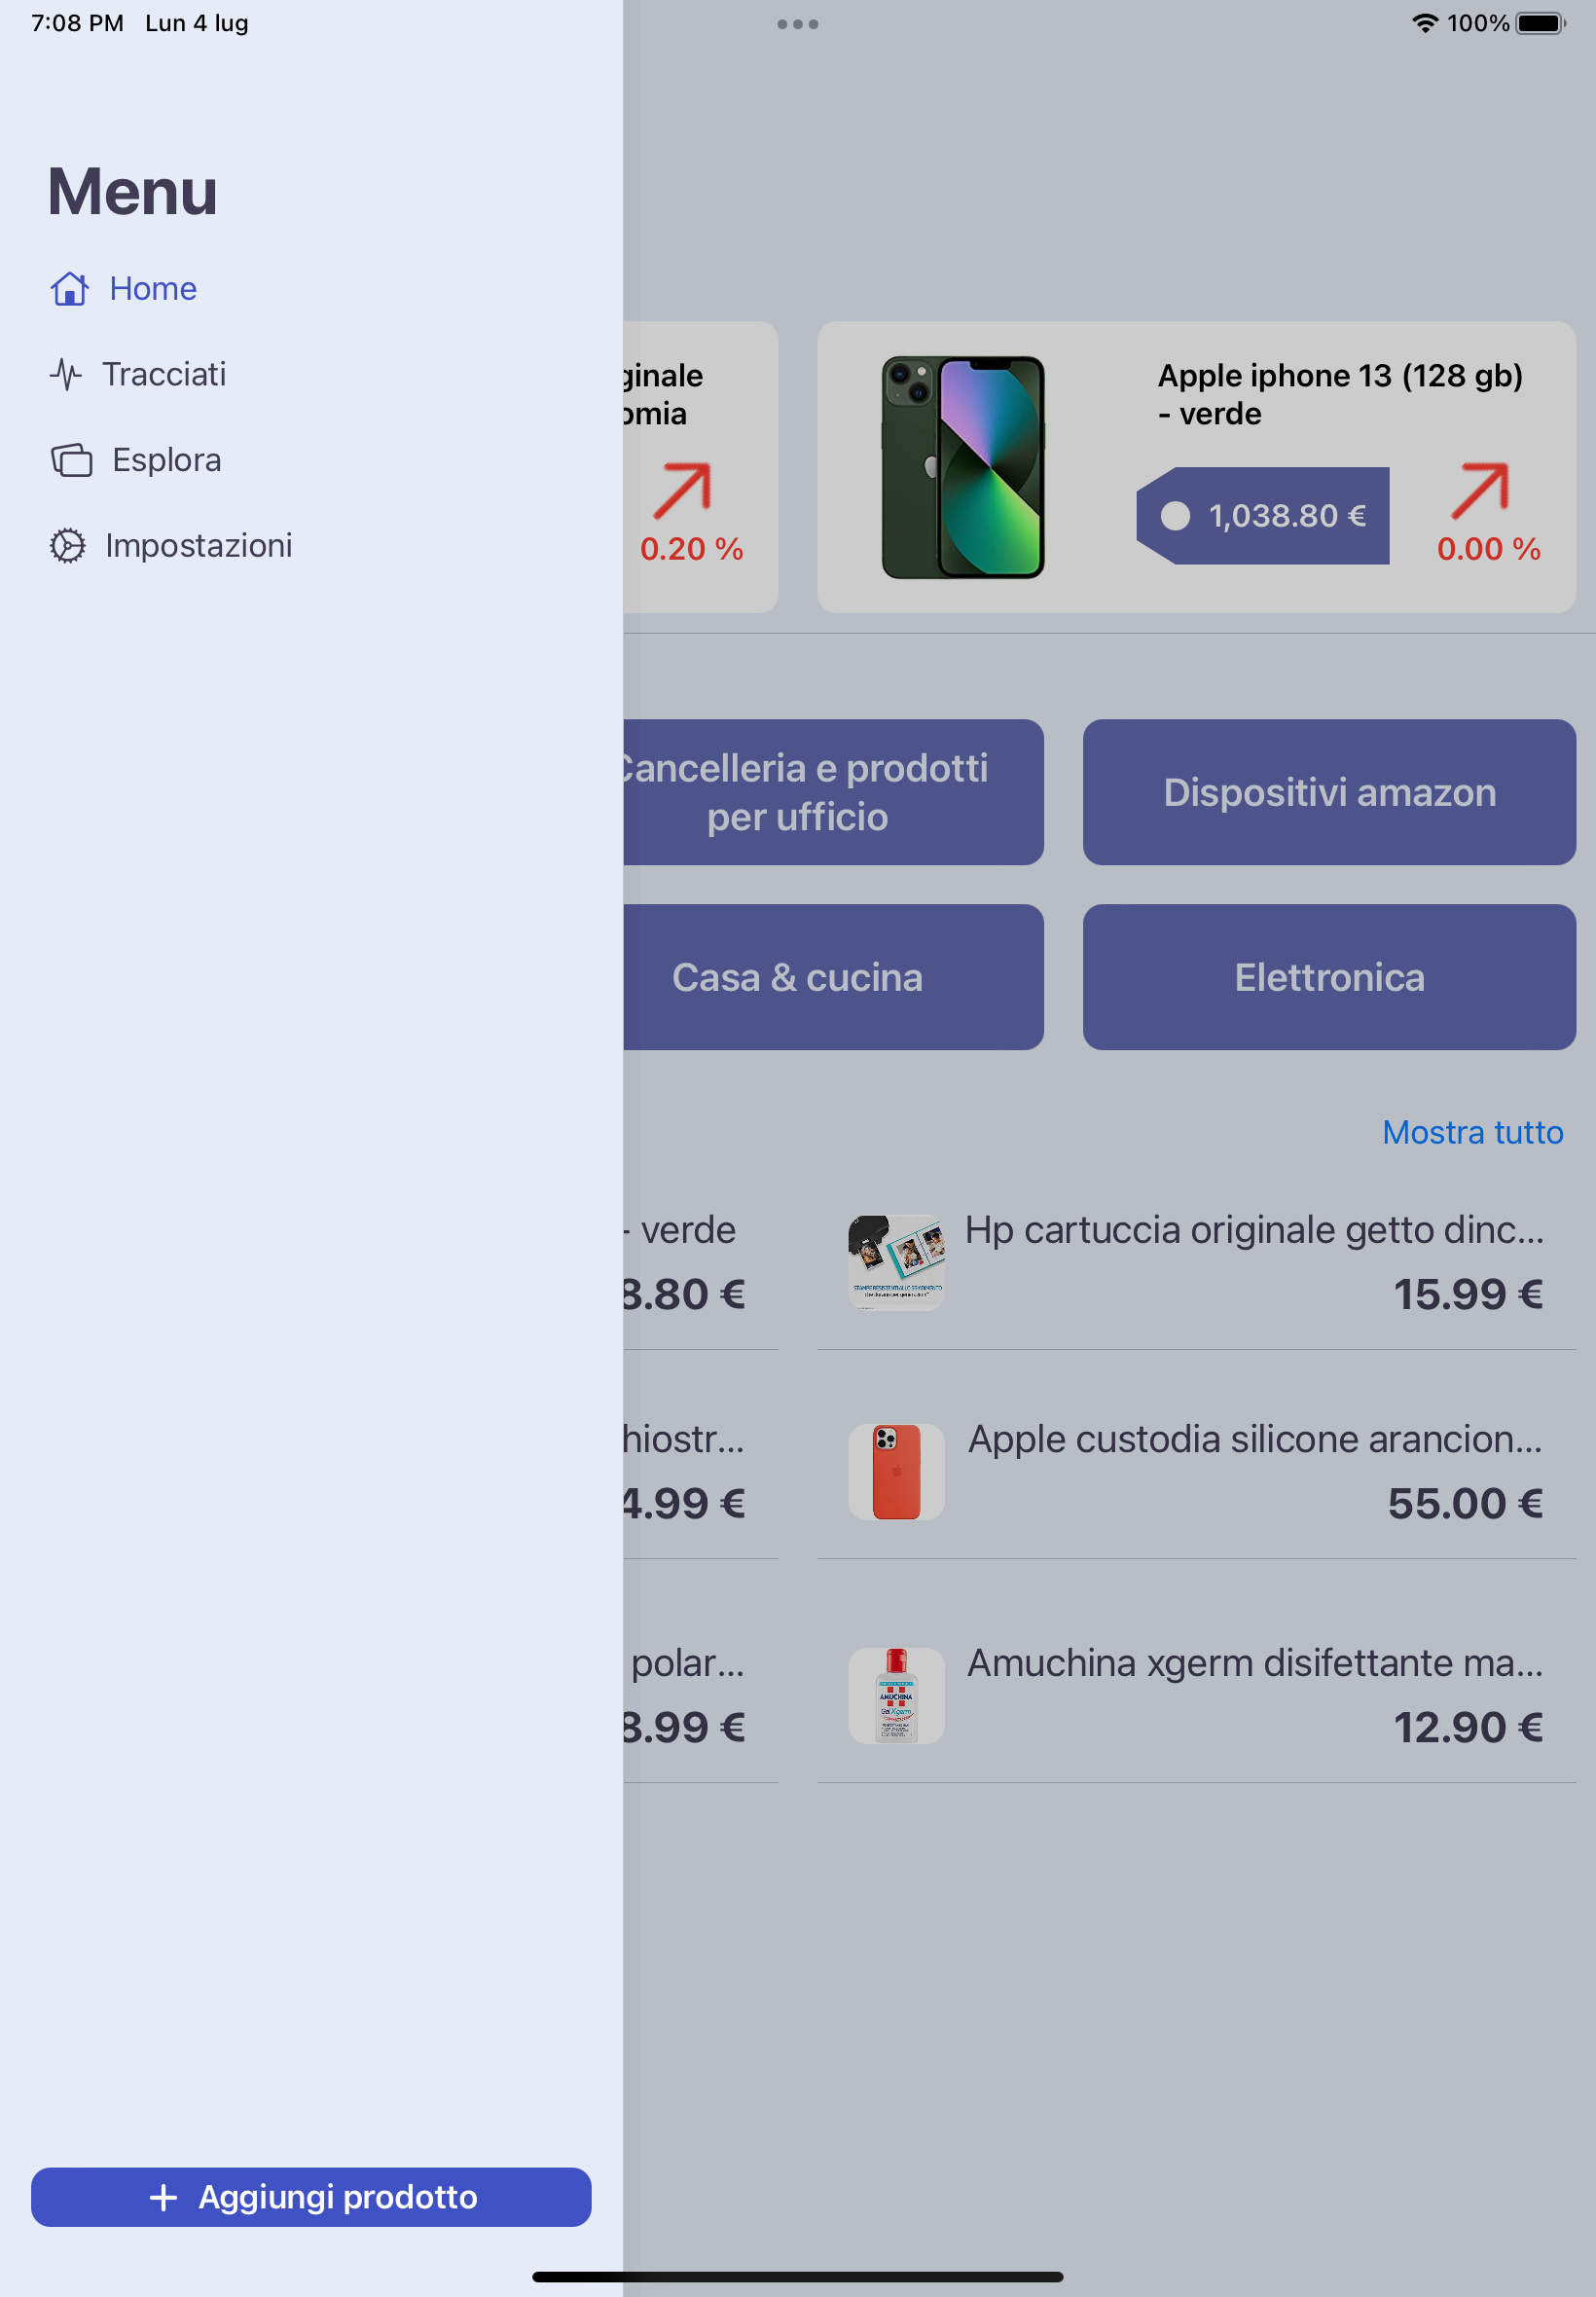
\includegraphics[scale=0.15]{images/interfaces/menu_ipad.png}
        \caption{Menu iPad screen}
        \label{fig:menu_ipad}
\end{figure}
\FloatBarrier
An additional screen is required to be shown for iPad. This screen is regarding the menu. From here the user can navigate throughout the application.



\newpage
\subsection{Views used}
The following views are sub-view (component) of the views described before.
\begin{itemize}
    \item {
        The bottom TabBar View (present only for iPhone) contains different section that the user can navigate:
        \begin{itemize}
            \item \textbf{Home:} The main page of the application
            \item \textbf{Tracking:} The view where products tracked by the logged user are visible
            \item \textbf{Explore:} The view in which there are some suggestion of products divided in different section.
            \item \textbf{Settings:} The view that let the user to customize settings of the application.
        \end{itemize}
        This view has been used in the main views of the application. Precisely in the Home view, tracked product view, explore view and settings view (fig: \ref{fig:home_screen} \& \ref{fig:tracking_product_screen} \& \ref{fig:explore_screen} \& \ref{fig:settings_screen}).
    }
    \item {
        The graph view is used to show the ongoing price of each product.
        This view has been used in the home of each product (fig: \ref{fig:product_screen}).
    }
    \item {
        The prices history view (fig: \ref{fig:product_screen}) List that shows all the prices since the product has been added to the application the first time, each cell row has also an arrow that goes up or down, if the price of the product is increased or decreased. If the price is not changed a - symbol is shown.
        This view has been used in the home of each product (fig: \ref{fig:product_screen}).
    }
    \item {
        The HGrid view displays products in a horizontal ScrollView and it is used to show the most tracked product in the home of the application (fig: \ref{fig:home_screen}).
    }
    \item {
        The infinite scroll view displays N products in a vertical List (using a paging mechanism), when the user reach one of the last products, a new request for the successive page will be done and N more elements will be added to the vertical stack, until no more element will be available.
        This view has been used  in the see all view of the explore section (fig: \ref{fig:see_all_explore_screen}).
    }
    \item {
        The image visualization view (fig: \ref{fig:detail_product_screen}) displays some images and let the user swipe horizontally between them.
        This view has been used in the detail section of a product (fig: \ref{fig:detail_product_screen}).
    }
    \item {
        The search bar view let the user write in it, binding the searched text with the view model.
        This view has been used in the user tracked product view (fig: \ref{fig:user_tracked_screen}).
    }
    \item {
        The percentage circular slider view let the user slide on a semicircular slide to get a percentage value.
        This view has been used in the percentage view to decide when receive the notification (fig: \ref{fig:percentage_notification_screen}).
    }
    \item {
        The vertical picker view let the user pick two different value, in order to form a price, with two different pickers.
        This view has been used in the value view to decide when receive the notification (fig: \ref{fig:value_notification_screen}).
    }
    \item {
        The price tag view creates a visual price tag.
        This view has been used in the home of the application (fig: \ref{fig:home_screen}).
    }
    \item {
        The last tracked product view has only one product displayed per time, to see the other product the user needs to slide horizontally.
        This view have different element inside:
        \begin{itemize}
            \item \textbf{Price tag:} with the actual price of a product.
            \item \textbf{Image of the product}. 
            \item \textbf{Name of the product}.
            \item \textbf{Ongoing of the product:} an arrow that goes up or down, if the price of the product is increased or decreased, with the percentage below it. If the price product has not been modified a - symbol is shown.
        \end{itemize}
        This view has been used in the home of the application (fig: \ref{fig:home_screen}).
    }
    \item {
        The single comment view show a comment of a user. In this view is present: the username of the user that has published the comment with his avatar, the comment text, the date when the comment has been published and 3 dot symbol (visible only if the current user is also the comment creator) that allow the him to modify or delete the comment.
        This view has been used in the comment section of a product (fig: \ref{fig:comments_product_screen}).
    }
    \item {
        Since SwiftUI doesn't provide a WebView, the WebView View is a UIViewRepresentable used to create a bridge between UIKit framework component (WKWebView) and SwiftUI. The UIViewRepresentable let also to connect the ViewModel used in SwiftUI view with the function implemented in the UIViewController by means of the Coordinator class that is the class in which the WKNavigationDelegate is implemented.
        This view has been used to show the Amazon website), through the click of the + button in the TabBar view; for that reason this view can be accessed from all the main views of the application (fig: \ref{fig:home_screen} \& \ref{fig:tracking_product_screen} \& \ref{fig:explore_screen} \& \ref{fig:settings_screen}).
    }
    \item {
        The loading indicator view is a view with an animation that shows the user that some loading is ongoing in the app.
        This view has been used in all the views the require a loading screen. For instance all the view that load content from the API.
    }
\end{itemize}


\newpage
\subsection{Widget view used}

Those are the available widgets for myAPTracker (figs: \ref{fig:small_medium_widget_view} \& \ref{fig:large_widget_view}).\\
From here the user can keep under control the price and the graph of some products; also the user can access the product in myAPTracker by directly clicking on them.
\begin{figure}[h!]
        \centering
        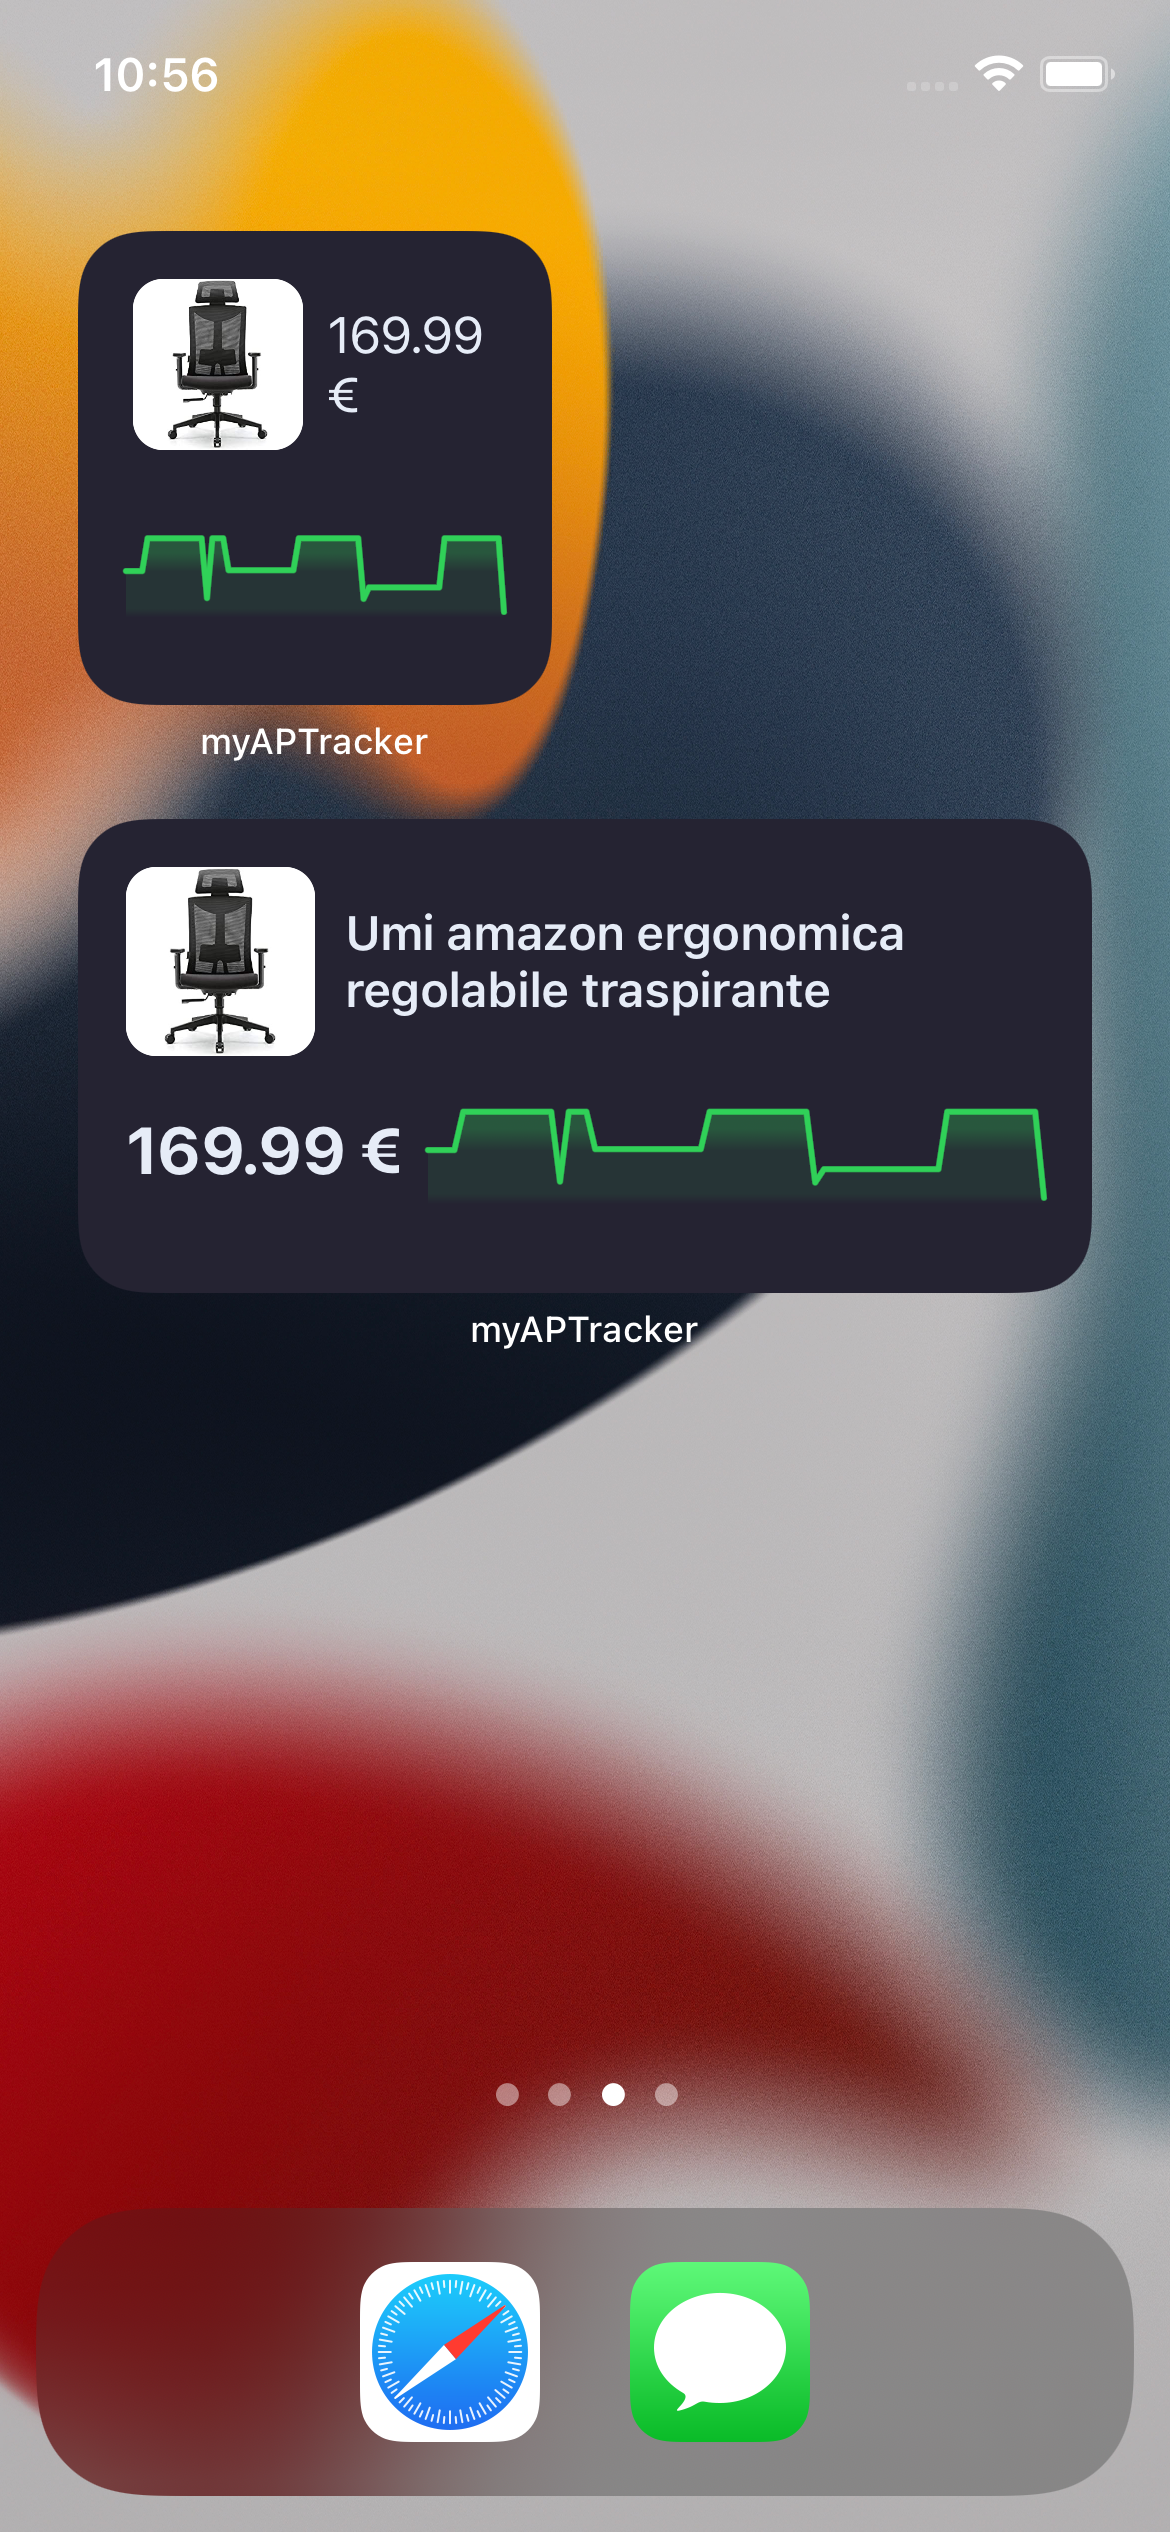
\includegraphics[scale=0.15]{images/interfaces/small_medium_widget_view.png}
        \caption{Small and medium widgets views}
        \label{fig:small_medium_widget_view}
\end{figure}
\FloatBarrier

\begin{figure}[h!]
        \centering
        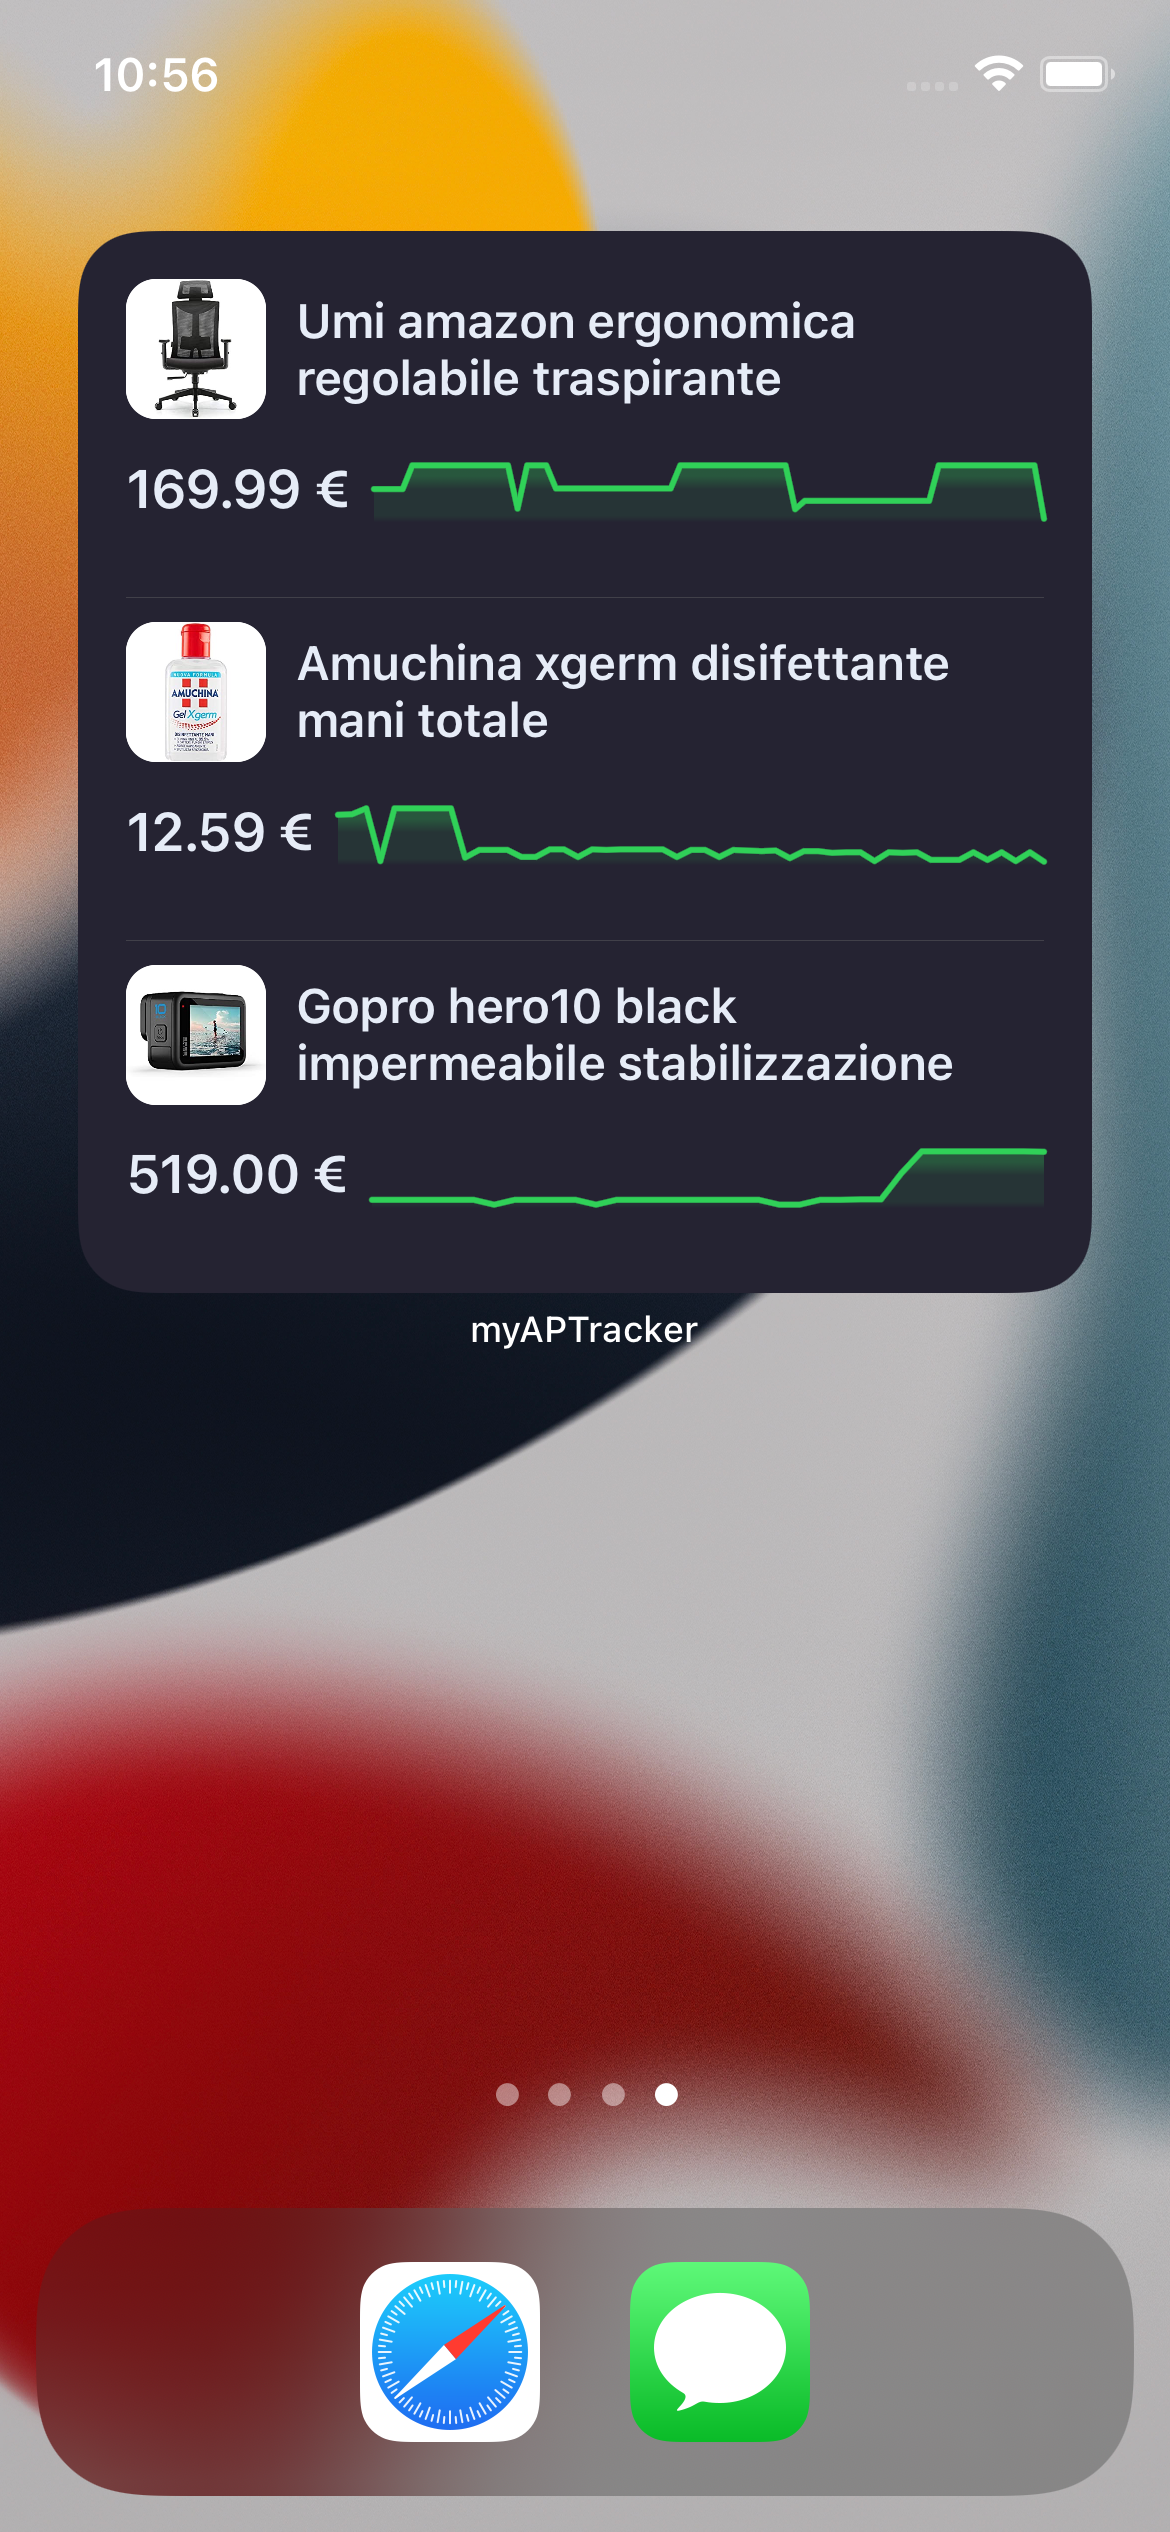
\includegraphics[scale=0.15]{images/interfaces/large_widget_view.png}
        \caption{Large widget view}
        \label{fig:large_widget_view}
\end{figure}
\FloatBarrier

\subsection{Apple Watch Application}
In order to have a quick access to the most important section of the application, we have also provided a simple application for the Apple Watch.\\
In this application the user can see the 10 most tracked products and the top 10 products with the highest percentage price drop.\\
Finally, if the user is logged in his iPhone, he can see all his tracked products in his wrist.

\begin{figure}[h!]
        \centering
        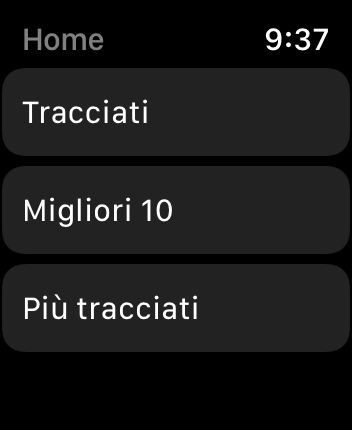
\includegraphics[width=0.3\textwidth]{images/interfaces/watch_home.png}
         \caption{Apple watch home}
        \label{fig:watch_home}
\end{figure}
\FloatBarrier
In figure \ref{fig:watch_home} is shown the home of the application. This view is composed by the three possible sections that the user can navigate.

\begin{figure}[h!]
        \centering
        \begin{subfigure}[b]{0.3\textwidth}
            \centering
            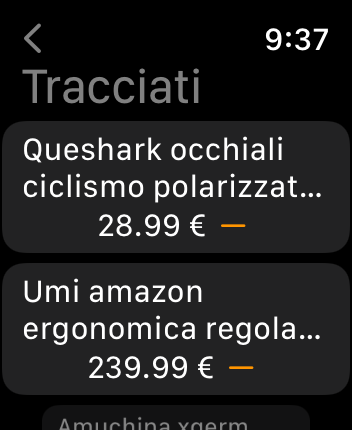
\includegraphics[width=\textwidth]{images/interfaces/watch_list_1.png}
        \end{subfigure}
        \begin{subfigure}[b]{0.3\textwidth}
            \centering
            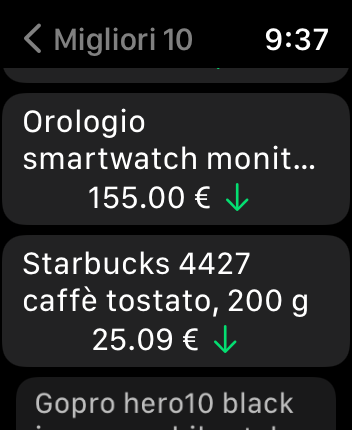
\includegraphics[width=\textwidth]{images/interfaces/watch_list_2.png}
        \end{subfigure}
         \caption{Apple watch list}
        \label{fig:watch_list}
\end{figure}
\FloatBarrier
In figure \ref{fig:watch_list} is shown how each one of the three sections display the products. For every product the name and the current price is reported with a symbol which indicates if the price has fallen down (bottom green arrow), the price is growth (up red arrow) or it remained constant (orange dash).

\begin{figure}[h!]
        \centering
        \begin{subfigure}[b]{0.3\textwidth}
            \centering
            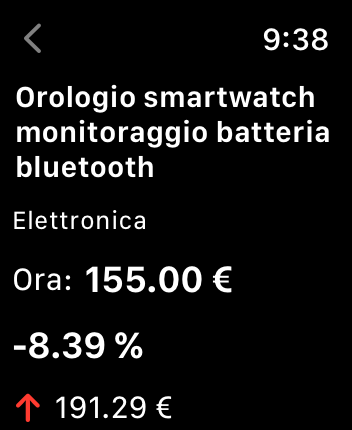
\includegraphics[width=\textwidth]{images/interfaces/watch_product_1.png}
        \end{subfigure}
        \begin{subfigure}[b]{0.3\textwidth}
            \centering
            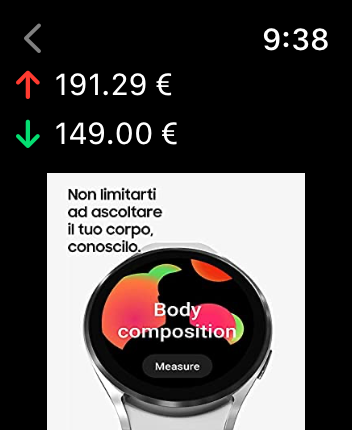
\includegraphics[width=\textwidth]{images/interfaces/watch_product_2.png}
        \end{subfigure}
        
         \caption{Product Screen}
        \label{fig:watch_product_screen}
\end{figure}
\FloatBarrier
In figure \ref{fig:watch_product_screen} is shown how the product screen looks like. Since in the Apple Watch the space is limited not all the information available in the iOS application were reported.\\
We decide to display the most relevant information for a user such as the name (with the category), the current price and the current discount if available, the highest and the lowest price in the product history and some images to better identify the product.